\documentclass[11pt]{book}

\typeout{new file: RadCal_User_Guide.tex}

%%%%%%%%%%%%%%%%%%%%%%%%%%%%%%%%%%%%%%%%%%%%%%%%%%%%%%%%%%%%%%%%%%%%%%%%%%%%%%%%%%%%%%%%%%%%%%%%%%%
%                                                                                                 %
% The mathematical style of these documents follows                                               %
%                                                                                                 %
% A. Thompson and B.N. Taylor. The NIST Guide for the Use of the International System of Units.   %
%    NIST Special Publication 881, 2008.                                                          %
%                                                                                                 %
% http://www.nist.gov/pml/pubs/sp811/index.cfm                                                    %
%                                                                                                 %
%%%%%%%%%%%%%%%%%%%%%%%%%%%%%%%%%%%%%%%%%%%%%%%%%%%%%%%%%%%%%%%%%%%%%%%%%%%%%%%%%%%%%%%%%%%%%%%%%%%

%%%%%%%%%%%%%%%%%%%%%%%%%%%%%%%%%%%%%%%%%%%%%%%%%%%%%%%%%%%%%%%%%%%%%%%%%%%%%%%%%%%%%%%%%%%%%%%%%%%
%                                                                                                 %
% The mathematical style of these documents follows                                               %
%                                                                                                 %
% A. Thompson and B.N. Taylor. The NIST Guide for the Use of the International System of Units.   %
%    NIST Special Publication 881, 2008.                                                          %
%                                                                                                 %
% http://www.nist.gov/pml/pubs/sp811/index.cfm                                                    %
%                                                                                                 %
%%%%%%%%%%%%%%%%%%%%%%%%%%%%%%%%%%%%%%%%%%%%%%%%%%%%%%%%%%%%%%%%%%%%%%%%%%%%%%%%%%%%%%%%%%%%%%%%%%%

\usepackage{times,mathptmx}
\usepackage[pdftex]{graphicx}
\usepackage{tabularx}
\usepackage{multirow}
\usepackage{booktabs}
\usepackage{pdfsync}
\usepackage{tikz}
\usepackage{color}
\usepackage{amsmath}
\definecolor{linknavy}{rgb}{0,0,0.50196}
\definecolor{linkred}{rgb}{1,0,0}
\definecolor{linkblue}{rgb}{0,0,1}
\usepackage{float}
\usepackage{caption}
\usepackage{graphpap}
\usepackage{rotating}
\usepackage{graphicx}
\usepackage{geometry}
\usepackage{relsize}
\usepackage{longtable}
\usepackage{amssymb}
\usepackage{makeidx} % Create index at end of document
\usepackage{lastpage} % Automatic last page number reference.
\usepackage[T1]{fontenc}
\usepackage{enumerate}
\usepackage{upquote}
\usepackage[section]{placeins}

\newcommand{\nopart}{\expandafter\def\csname Parent-1\endcsname{}} % To fix table of contents in pdf.
\newcommand{\ct}{\tt\small} % eventually will be deprecated due to http://www.tex.ac.uk/cgi-bin/texfaq2html?label=2letterfontcmd
\newcommand{\textct}[1]{\texttt{\small #1}}

\usepackage{tocstyle} % Fix table of contents sections from overlapping section titles
\usetocstyle{standard}
\usepackage{listings}
\usepackage{textcomp}
\definecolor{lbcolor}{rgb}{0.96,0.96,0.96}

\lstset{
    %backgroundcolor=\color{lbcolor},
    tabsize=4,
    rulecolor=,
    language=Fortran,
        basicstyle=\footnotesize\ttfamily,
        upquote=true,
        aboveskip={\baselineskip},
        belowskip={\baselineskip},
        columns=fixed,
        extendedchars=true,
        breaklines=true,
        breakatwhitespace=true,
        frame=none,
        showtabs=false,
        showspaces=false,
        showstringspaces=false,
        identifierstyle=\ttfamily,
        keywordstyle=\color[rgb]{0,0,0},
        commentstyle=\color[rgb]{0,0,0},
        stringstyle=\color[rgb]{0,0,0},
}

\usepackage[pdftex,
        colorlinks=true,
        urlcolor=linkblue,     % \href{...}{...} external (URL)
        citecolor=linkred,     % citation number colors
        linkcolor=linknavy,    % \ref{...} and \pageref{...}
        pdfproducer={pdflatex},
        pagebackref,
        pdfpagemode=UseNone,
        bookmarksopen=true,
        plainpages=false,
        verbose]{hyperref}

\setlength{\textwidth}{6.5in}
\setlength{\textheight}{9.0in}
\setlength{\topmargin}{0.in}
\setlength{\headheight}{0.in}
\setlength{\headsep}{0.in}
\setlength{\parindent}{0.25in}
\setlength{\oddsidemargin}{0.0in}
\setlength{\evensidemargin}{0.0in}
\setlength{\leftmargini}{\parindent} % Controls the indenting of the "bullets" in a list

\newcommand{\titlesigs}
{
\small
\flushright{U.S. Department of Commerce \\
{\em Wilbur L. Ross, Jr., Secretary} \\
\hspace{1in} \\
National Institute of Standards and Technology \\
{\em Walter Copan, NIST Director and Undersecretary of Commerce for Standards and Technology} }
}


\newcommand{\dod}[2]{\frac{\partial #1}{\partial #2}}
\newcommand{\DoD}[2]{\frac{\mathrm{D} #1}{\mathrm{D} #2}}
\newcommand{\dsods}[2]{\frac{\partial^2 #1}{\partial #2^2}}
\renewcommand{\d}{\,\mathrm{d}}
\newcommand{\dx}{\delta x}
\newcommand{\dy}{\delta y}
\newcommand{\dz}{\delta z}
\newcommand{\degF}{$^\circ$F}
\newcommand{\degC}{$^\circ$C}
\newcommand{\x}{x}
\newcommand{\y}{y}
\newcommand{\z}{z}
\newcommand{\dt}{\delta t}
\newcommand{\dn}{\delta n}
\newcommand{\cH}{H}
\newcommand{\hu}{u}
\newcommand{\hv}{v}
\newcommand{\hw}{w}
\newcommand{\la}{\lambda}
\newcommand{\bO}{{\Omega}}
\newcommand{\bo}{{\mathbf{\omega}}}
\newcommand{\btau}{\mathbf{\tau}}
\newcommand{\bdelta}{{\mathbf{\delta}}}
\newcommand{\sumyw}{\sum (Y_\alpha/W_\alpha)}
\newcommand{\oW}{\overline{W}}
\newcommand{\om}{\ensuremath{\omega}}
\newcommand{\omx}{\omega_x}
\newcommand{\omy}{\omega_y}
\newcommand{\omz}{\omega_z}
\newcommand{\erf}{\hbox{erf}}
\newcommand{\erfc}{\hbox{erfc}}
\newcommand{\bF}{{\mathbf{F}}}
\newcommand{\bG}{{\mathbf{G}}}
\newcommand{\bof}{{\mathbf{f}}}
\newcommand{\bq}{{\mathbf{q}}}
\newcommand{\br}{{\mathbf{r}}}
\newcommand{\bu}{{\mathbf{u}}}
\newcommand{\bx}{{\mathbf{x}}}
\newcommand{\bk}{{\mathbf{k}}}
\newcommand{\bv}{{\mathbf{v}}}
\newcommand{\bg}{{\mathbf{g}}}
\newcommand{\bn}{{\mathbf{n}}}
\newcommand{\bS}{{\mathbf{S}}}
\newcommand{\bW}{\overline{W}}
\newcommand{\dS}{d{\mathbf{S}}}
\newcommand{\bs}{{\mathbf{s}}}
\newcommand{\bI}{{\mathbf{I}}}
\newcommand{\hp}{H}
\newcommand{\trho}{\tilde{\rho}}
\newcommand{\dph}{{\delta\phi}}
\newcommand{\dth}{{\delta\theta}}
\newcommand{\tp}{\tilde{p}}
\newcommand{\bp}{\overline{p}}
\newcommand{\dQ}{\dot{Q}}
\newcommand{\dq}{\dot{q}}
\newcommand{\dbq}{\dot{\mathbf{q}}}
\newcommand{\dm}{\dot{m}}
\newcommand{\ha}{\frac{1}{2}}
\newcommand{\ft}{\frac{4}{3}}
\newcommand{\ot}{\frac{1}{3}}
\newcommand{\fofi}{\frac{4}{5}}
\newcommand{\of}{\frac{1}{4}}
\newcommand{\twth}{\frac{2}{3}}
\newcommand{\R}{R}
\newcommand{\be}{\begin{equation}}
\newcommand{\ee}{\end{equation}}
\newcommand{\RE}{\hbox{Re}}
\newcommand{\LE}{\hbox{Le}}
\newcommand{\PR}{\hbox{Pr}}
\newcommand{\PE}{\hbox{Pe}}
\newcommand{\NU}{\hbox{Nu}}
\newcommand{\SC}{\hbox{Sc}}
\newcommand{\SH}{\hbox{Sh}}
\newcommand{\WE}{\hbox{We}}
\newcommand{\COTWO}{\text{\tiny \hbox{CO}$_2$}}
\newcommand{\HTWOO}{\text{\tiny \hbox{H}$_2$\hbox{O}}}
\newcommand{\OTWO}{\text{\tiny \hbox{O}$_2$}}
\newcommand{\NTWO}{\text{\tiny \hbox{N}$_2$}}
\newcommand{\CO}{\text{\tiny \hbox{CO}}}
\newcommand{\F}{\text{\tiny \hbox{F}}}
\newcommand{\C}{\text{\tiny \hbox{C}}}
\newcommand{\Hy}{\text{\tiny \hbox{H}}}
\newcommand{\So}{\text{\tiny \hbox{S}}}
\newcommand{\M}{\text{\tiny \hbox{M}}}
\newcommand{\xx}{\text{\tiny \hbox{x}}}
\newcommand{\yy}{\text{\tiny \hbox{y}}}
\newcommand{\zz}{\text{\tiny \hbox{z}}}

\newcommand{\calH}{\mathcal{H}}
\newcommand{\calR}{\mathcal{R}}

\newcommand{\dif}{\mathrm{d}}
\newcommand{\Div}{\nabla\cdot}
\newcommand{\D}{\mbox{D}}
\newcommand{\mhalf}{\mbox{$\frac{1}{2}$}}
\newcommand{\thalf}{\mbox{\tiny $\frac{1}{2}$}}
\newcommand{\tripleprime}{{\prime\prime\prime}}
\newcommand{\ppp}{{\prime\prime\prime}}
\newcommand{\pp}{{\prime\prime}}

\newcommand{\superscript}[1]{\ensuremath{^{\textrm{\tiny #1}}}}
\newcommand{\subscript}[1]{\ensuremath{_{\textrm{\tiny #1}}}}

\newcommand{\rb}[1]{\raisebox{1.5ex}[0pt]{#1}}

\newcommand{\Ra}{$\Rightarrow$}
\newcommand{\hhref}[1]{\href{#1}{{\tt #1}}}
\newcommand{\fdsinput}[1]{{\scriptsize\verbatiminput{../../Verification/Visualization/#1}}}

\floatstyle{boxed}
\newfloat{notebox}{H}{lon}
\newfloat{warning}{H}{low}


\IfFileExists{gitrevision.tex}
{\input{gitrevision}}
{\newcommand{\gitrevision}{unknown} }

\begin{document}

\bibliographystyle{unsrt}

\pagestyle{empty}

\begin{minipage}[t][9in][s]{6.25in}

\huge \flushright{\bf NIST Technical Note 1402 \\ \Large Second Edition}

\vspace{1in}

\Huge \flushright{\bf RadCal: A Narrow-Band Model \\ for Radiation Calculations \\ in a Combustion Environment}

\vfill

\large
\flushright{ 
William L. Grosshandler \\
Vivien R. Lecoustre }

\normalsize
\vfill

\flushright{

\includegraphics[width=2.in]{Figures/nistident_flright_vec}
}

\end{minipage}

\newpage

\hspace{5in}

\newpage

\begin{minipage}[t][9in][s]{6.25in}

\huge \flushright{\bf NIST Technical Note 1402 \\ \Large Second Edition}

\vspace{.75in}

\Huge \flushright{\bf  RadCal: A Narrow-Band Model \\ for Radiation Calculations \\ in a Combustion Environment}

\vspace{.25in}
\large 
\flushright{William L. Grosshandler \\
Vivien R. Lecoustre}

\normalsize
\vspace{.25in}

\flushright{
Fire Research Division \\
Engineering Laboratory  \\
{\em Gaithersburg, Maryland, USA}}

\vspace{.25in}

\flushright{\today \\
\emph{Revision:~\gitrevision}}

\vfill

\flushright{
\includegraphics[width=1.2in]{Figures/doc} }

\titlesigs

\end{minipage}

\newpage

\begin{minipage}[t][9in][s]{6.25in}

\flushright{Certain commercial entities, equipment, or materials may be identified in this \\
document in order to describe an experimental procedure or concept adequately. \\
Such identification is not intended to imply recommendation or endorsement by the \\
National Institute of Standards and Technology, nor is it intended to imply that the \\
entities, materials, or equipment are necessarily the best available for the purpose.
}

\vspace{3in}

\large
\flushright{\bf National Institute of Standards and Technology Technical Note \\
Natl.~Inst.~Stand.~Technol.~Tech.~Note, \pageref{LastPage} pages (August 2020) \\
CODEN: NSPUE2 }

\vfill

\hspace{1in}

\end{minipage}

\newpage

\frontmatter

\pagestyle{plain}

\chapter{Abstract}

RadCal is a narrow-band radiation solver for combustion and fire applications. It spectrally solves the radiative transfer equation along a one-dimensional, line-of-sight in homogeneous and non-homogeneous semi-transparent media for conditions typical of fire and furnaces. Emphasis is on the infra-red part of the spectrum, although the user is free to defined the range of interest.

Originally developed with a spectral characterization of $\rm CO_2$, CO, $\rm H_2O$, $\rm CH_4$, and soot, the code has been enhanced with the addition of new species: $\rm C_2H_4$ (ethylene), $\rm C_2H_6$ (ethane), $\rm C_3H_6$ (propylene), $\rm C_3H_8$ (propane), $\rm C_7H_8$ (toluene), $\rm C_7H_{16}$ (\textit{n}-heptane), $\rm CH_3OH$ (methanol), and $\rm C_5H_8O_2$ (methyl methacrylate). The spectrum of these species can be calculated using Malkmus narrow-band parameters prepared from the experimental FTIR measurements of Wakatsuki and Yilmaz at ambient to elevated temperatures.

In addition to the addition of new species, significant modifications have been made to the numerical solver. The code has been entirely rewritten in modern Fortran to increase code readability, modularity, and to facilitate its integration within the NIST Fire Dynamics Simulator. The structure of the input file has been modified and the code now offers the possibility to compute the spectrum of any hydrocarbon mixture.

This report aims to provide a complete description of the models used in solving the radiative heat transfer equation. Emphasis is on the Lorentz line narrow-band models used in the code: Elsasser, Goody, and Malkmus. The report presents the different species that were already present in the original version of RadCal. It then presents the radiative coefficients for various fuels derived from FTIR experiments conducted at the National Institute of Standards and Technology. A description of the method used to extract the narrow-band coefficients is included, and these new narrow-band model coefficients, spectral mean absorption coefficients, and band overlap parameters are presented in detail for each of the new species, along with several verifications tests. This report also features a description of the new input file, a thorough presentation of the code structure, and several code verification and validation tests.

\chapter{Disclaimer}

The US Department of Commerce makes no warranty, expressed or implied,
to users of RadCal, and accepts no responsibility for its use.
Users of RadCal assume sole responsibility under Federal law for determining
the appropriateness of its use in any particular application;
for any conclusions drawn from the results of its use; and for any
actions taken or not taken as a result of analysis performed using these tools.

Users are warned that RadCal is intended for use only by those competent
in the fields of heat transfer and fire science,
and is intended only to supplement the informed judgment of the qualified user.
The software package is a computer model that may or may not have predictive
capability when applied to a specific set of factual circumstances.
Lack of accurate predictions by the model could lead to erroneous
conclusions with regard to fire safety. All results should be evaluated by an informed user.

Throughout this document, the mention of computer hardware or commercial
software does not constitute endorsement by NIST, nor does it indicate that
the products are necessarily those best suited for the intended purpose.


\chapter{Acknowledgments}

The authors would like to acknowledge the tremendous experimental work of Kaouru Wakatsuki and Aykut Yilmaz. Their experimental characterization of the infra-red spectrum of several hydrocarbons at different temperatures, under the careful supervision and help from Gregory Jackson and Anthony Hamins, has been the stepping stone of this version of RadCal. This work is the direct continuation of their experimental work. Finally, the authors are indebted to John De Ris and Robert Hall for kindly reviewing the manuscript.

\newpage

\tableofcontents

\mainmatter

% !TEX root = RadCal_User_Guide.tex

\typeout{new file: Introduction_Chapter.tex}

\chapter{Introduction}

Thermal radiation fire plays a preponderant role in most fires as it is responsible for fire spread and fire growth due to thermal feedback from the hot upper layer in a compartment fire or the hot plume in an open pool fire, or controls the mass loss rate in large scale pool fire.
In all the aforementioned cases, it is crucial to accurately determinate the radiative heat transfer. The use of the Wien's displacement law quantifies the wavelength of the maximum radiative energy emitted by a blackbody. This law is expressed
by
\begin{equation}\label{eq:Wien}
 \rm \lambda_m T = 2897 \, \mu m.K
\end{equation}
with $\rm \lambda_m$ being the wavelength in units of m, corresponding to the peak intensity of blackbody emittance; T represents the temperature in units of Kelvin of the blackbody. Equation \ref{eq:Wien} says that in typical fire configurations, where the temperature ranges from 300~K to about 2500~K, the peak emittance wavelength varies from 10 $\rm \mu m$ to 1.1 $\rm \mu m$: almost all the radiative exchanges happen in the near to mid infrared range. Most of the components involved in fire are present in gas phase. The infrared spectrum of the gases is very discontinuous, with few narrow spectral areas that participate to radiative exchange. The rest of the spectrum is practically transparent. The participation propensity varies with the amount of the species present and the local temperature.

These intrinsics aspects of the radiative exchange between medium with important gradients of temperature, species amount, and non-homogeneity in species render this problem quite complex and some level of sophistication is needed in its treatment. The radiative properties of a gas species are dictated by quantum mechanics and are related to the composition and the structure of the component considered. The discrete nature of the energy levels (mostly vibrational and rotational modes) for a given molecule generate its infrared ``fingerprint''. While a thorough consideration of all the energy levels would give an exact assessment of the radiative exchange -- this is often referred to as line-by-line calculation in the literature -- this operating mode is still too computationally expensive for engineering applications and is only used for simple configurations. Moreover, the lack of data for both elevated temperatures and for most hydrocarbon species further restricts its applicability to fire scenarios. The development of narrow-band models constitutes a compromise between accuracy and efficiency. Narrow-band models divide the spectrum of interest into small spectral segments of uniform spectral properties and use statical representations of the energy levels over these segments. Narrow band models are computationally fast and accurate. In particular, they do not require detailed knowledge of all the active energy levels in a given molecule. They are easier to implement and use than Line-by-Line techniques.

RadCal was previously developed by Grosshandler \cite{Grosshandler1993} to predict radiative heat transfer from gases at elevated temperature using narrow-band models. RadCal is a computer program, originally written in FORTRAN 77, that computes the directional spectral intensity from a non-isothermal, non-uniform mixture of gases and soot, by spectrally solving the radiative transfer equation. In addition, RadCal returns the Planck mean absorption coefficient, an effective absorption coefficient, and other integrated quantities. Details about the different models used and the quantities printed by RadCal are provided in Chapter \ref{chap:SNB}.

The first version of RadCal was developed to predict the enhancement in radiation caused by the addition of pulverized coal to a 60 kW methanol-fired furnace~\cite{Grosshandler1976}. This first version considered the contributions of CO, $\rm CO_2$, $\rm H_2O$, and soot. Validation of first version of RadCal was documented in 1979 and can be found in Ref.~\cite{Grosshandler1979}. Predictions from RadCal for $\rm CO_2$, CO, and $\rm H_2O$ in individual or in mixtures were compared against published data. Good agreement was found except for some data. As Grosshandler states in Ref.~\cite{Grosshandler1993}:
\textit{``...The spectrum between 1.25 and 12.5 $\mu$m was satisfactorily reproduced, although some of the data at particular wavelengths differed from the prediction by as much as 17\%. Considerable disagreement occurred between the integrated emittance of $\rm CO_2$ as predicted from RADCAL and that computed from the charts of Hottel \cite{Hottel1954}. No one source for this disagreement was identified, but it was thought to be a combination of the difficulty in obtaining high accuracy spectral measurements under the full range of conditions investigated, the uncertainty associated with extrapolating total transmittance results beyond the measured temperature and pressure-pathlengths, and the approximations associated with the narrow-band models.''}

Methane was added to RadCal in 1985 \cite{Grosshandler1985}, along with an extension to 200 $\rm \mu m$ of the considered spectrum. The added methane data originates mostly from experiments performed by Brosmer \textit{et al.} \cite{Brosmer1985} and Lee \textit{et al.} \cite{Lee1964}. At this time, the code structure was updated and a new input file was created.

This report, a second edition of NIST Special Publication 1402, presents the latest enhancements brought to RadCal and aims to provide an exhaustive list of the mathematical and physical models used in RadCal, which was missing from the first edition. Chapter~\ref{chap:SNB} presents the fundamental mathematical models used in radiative heat transfer and presents the different narrow-band models used in RadCal. Chapter~\ref{chap:old_species} recalls the characteristics of the species that were present in the 1993 version of RadCal: $\rm H_2O$, $\rm CO_2$, CO, $\rm CH_4$, and soot. Additional hydrocarbons have been implemented into RadCal and the code has been rewritten, for its most part, into Fortran 2008. FTIR transmission measurements at the National Institute of Standards and Technology (NIST) were undertaken to provide highly resolved spectral absorption coefficients in the mid-IR and NIR as a function of temperature for many fuel species~\cite{Wakatsuki2005a,Wakatsuki2008,Yilmaz2008}. These measurements were performed over a range of temperatures from 300~K up to 1000~K for several fuel species, including paraffins (methane, ethane, propane, and n-heptane), olefins (ethylene and propylene), and other fuel-related species (methanol, toluene, and methyl-methacrylate). The uniform set of conditions and spectral resolution of these measurements have provided a set of data for developing calculation methodologies for absorption coefficients of these species in flame environments. New species and their associated narrow-band parameters are described in Chapter~\ref{chap:new_species}. The syntax of the input file was modified to make good use of native Fortran namelist that offers a more flexible way to input data. Chapter~\ref{chap::using_RADCAL} describes the new input file syntax, and how to compile and use RadCal. The code was modified following a modular approach and was translated into Fortran 2008 to benefit from recent advances in Fortran standard. The list of RadCal functions and subroutines is detailed in Chapter~\ref{chap:Code}.  The code has also been modified to account for any type of fuel mixture. Verification of the new species spectral data has been performed and results from these tests are reported in Chapter~\ref{sec:verification}. Finally, Chapter~\ref{chap::validation_tests} compares the new version of RadCal with the 1993 one for the various validation tests presented in the first edition of this report. This chapter also presents predicted quantities from an experimentally characterized small methanol pool fire.



Include here New RadCal features in a list:

\begin{itemize}
 \item New species spectral data between 700 and 4000~$\rm cm^{-1}$ and for temperature ranging from about 300~K to about 1000~K.
 \item New species data for: Ethylene, Ethane, Propylene, Propane, n-Heptane, Toluene, Methanol, Methane, MMA
 \item Code rewritten in Fortran 2008
 \item Code made modular
 \item More convenient input file
 \item Possibility to calculate the spectrum for any mixture of gas
 \item Updated and enhanced user guide
\end{itemize}


\typeout{new file: Band_Models_Chapter.tex}

\chapter{Narrow Band Models and Approximations}
\label{chap:SNB}

This chapter briefly presents the models and their formulations that are used in RadCal. The reader seeking further details on the rather complex theory behind these models is invited to read the exhaustive monographs from Penner~\cite{Penner1959}, Tien~\cite{Tien1968}, and Modest~\cite{Modest2013}, the reviews from De Ris~\cite{DeRis1979} and from Viskanta and Menguc~\cite{vm_87}, and the report from Ludwig \textit{et al.}~\cite{Ludwig1973}. Most of the equations used in RadCal can be found in the latter.

RadCal was designed for uses at moderate gas pressure (near atmospheric pressure) and for ambient to high gas temperatures (typically from around 300~K to 2500~K). As such, collision broadening is the main broadening mechanism considered. However, the effects of Doppler line broadening, which are common at low pressure (typically less than 0.01 atm) and/or at high temperature, are still accounted for in the overall expression of narrow-band transmissivity. The Doppler broadening effect is accounted using the method presented in Ludwig \textit{et al.}~\cite{Ludwig1973}. The Voigt profile, commonly used in atmospheric sciences~\cite{Chu1994}, is not considered here. Unlike the Lorentz profile the Voigt profile does not have a closed analytical expression. Effects of scattering or reflection are not included in RadCal; as such, RadCal considers only absorption and emission.

RadCal can be used to model homogeneous and non-homogeneous conditions. Following Ludwig~\cite{Ludwig1973}, the Curtis-Godson approximation is then used with the assumption of Single Line Group. In the case of a mixture of different radiative participating gases, the contribution for each species is calculated independently and their contribution on the total spectral optical depth is assumed to be additive. Finally, it is important to recall the important assumption of local thermodynamic equilibrium used in establishing the Radiative Transfer Equation as solved by RadCal. This justifies consideration of the Planck blackbody distribution law for the emission term.

\section{Introduction}

\subsection{Radiative Transfer Equation (RTE)}
The expression of the equation of transfer in non-scattering, participating media in local thermodynamic equilibrium is recalled. This equation is the mathematical foundation of RadCal. The Eulerian point of view is adopted here. The assumption of local thermodynamic equilibrium has for consequences that the spectral blackbody emission can be modeled with the Planck blackbody distribution - denoted from here and in the rest of this manuscript $I_b$, and that the Kirchoff law applies at the spectral level, \textit{i.e.} for a monochromatic light the absorption and emission coefficients are equal. The amount of radiative energy emitted by a participating medium of local thermodynamic temperature $T$, over an infinitesimal spectrum $\d\nu$, in an arbitrary direction $\hat{\textbf{s}}$, and along an infinitesimal length $\d s$, is expressed by:
\begin{equation}\label{eq:emission}
 j_{e,\nu} \d s \d\nu = \kappa_{\nu} I_{\rm b,\nu}(T)\d\nu \d s
\end{equation}
where $j_{e,\nu}$ is the emission at the frequency $\nu$, $\kappa_{\nu}$ is the absorption coefficient at the considered frequency, $I_{b,\nu}$ denotes the spectral intensity emitted by a blackbody of temperature $T$. Naturally, the absorption coefficient $\kappa_{\nu}$ is proportional to the amount of local participating molecule.


Note: it is common in spectroscopy to use $B_b$ and $\tilde{\nu}$ as the Planck function and wavenumber, respectively. However in the continuation of the previous work on RadCal, we keep the previously used nomenclature. In the rest of the manuscript, $\omega$ denotes the wavenumber. A common units employs to characterize radiative spectrum is the wavelength, denoted $\la$. Wavelength $\la$ represents the distance traveled during one cycle when propagating at the speed of light in vacuum. When dealing with infrared radiation, its units are commonly expressed in ${\rm \mu m}$. Wavenumber $\om$ is the reciprocal of the wavelength. It represents the number of cycles per unit of length. It is expressed in units of ${\rm cm^{-1}}$. It is convenient to use wavelength $\la$ or wavenumber $\om$ instead of frequency $\nu$ when dealing with thermal radiation. Wavenumber and wavelength are related to frequency through:
\be
 \la = c/\nu \: \: \rm{and} \: \: \om = \nu /c,
\ee
 and one can easily switch from wavenumber in units of ${\rm cm^{-1}}$ to wavelength in units of ${\rm \mu m}$ with:
\be
  \la \; {\rm \mu m}  \; = 10000/\om \; \; {\rm cm^{-1}}.
\ee

Similarly to Eq.~\ref{eq:emission}, an expression characterizing the amount of energy of an incident beam, of propagating direction $\hat{\textbf{s}}$ absorbed by local participating molecules over an infinitesimal spectrum $\d\nu$ and along an infinitesimal length $\d s$ can be derived:
\begin{equation}\label{eq:absorption}
  j_{a,\nu} \d\nu \d \rm s = - \kappa_{\nu} I_{\nu} \d\nu \d \rm s
\end{equation}
where $I_{\nu}$ is the spectral intensity at frequency $\nu$ of the incident beam of direction $\vec{\textbf{s}}$.

Using Eqs.~\ref{eq:emission} and \ref{eq:absorption}, the change in the spectral intensity of an incident beam of direction $\hat{\textbf{s}}$ penetrating a participating medium over a distance $\d s$ is then expressed by:
\be
\d I_{\nu}\d \nu = (j_{e,\nu} + j_{a,\nu}) \d s \d\nu.
\ee
The local Radiative Transfer Equation (neglecting scattering) is then expressed as:
\begin{equation}\label{eq:localRTE}
 \dfrac{\d I_{\nu}}{\d s}\d \nu = \kappa_{\nu} (I_{\rm b,\nu}(T) - I_{\nu}) \d \nu.
\end{equation}
Equation~\ref{eq:localRTE} is a first-order ordinary differential equation; it is assumed here that the speed of light is very large compared to local time and length scales involved. The functional form of the spectral intensity $I_{\nu}(s)$ at an arbitrary depth $s$ within the participating medium, assuming that the participating medium starts at $s=0$, is expressed as:
\begin{equation}\label{eq:RTE_Kappa}
I_{\nu}(s) =  I_{\nu}(0) \exp\left(-\displaystyle\int_{0}^{s}{\kappa_{\nu}\d s}'\right) + \displaystyle\int_0^{s}{I_{\rm b,\nu}\left(T(s')\right)\exp\left(-\displaystyle\int_{s'}^{s}{\kappa_{\nu}\d s''}  \right)\kappa_{\nu} \d s'}.
\end{equation}
Note that $\kappa_{\nu}$ is a function of the local thermodynamic conditions and hence is an implicit function of $s$.

The first right-hand side term of Eq.~\ref{eq:RTE_Kappa} represents the fraction of the incident spectral intensity that is transmitted unto the depth $s$. The second right-hand side term corresponds to the contribution of the local emission and accounts for self-absorption.
The spectral transmissivity, denoted $\tau(\nu; 0 \rightarrow s)$, is defined as the fraction of the spectral energy of frequency $\nu$ incident upon a participating medium which is transmitted by it. It can be seen from Eq.~\ref{eq:RTE_Kappa}, that an explicit formulation of the spectral transmissivity is:
\begin{equation}\label{eq:tau_definition}
 \tau(\nu; 0 \rightarrow s) = \exp\left(-\displaystyle\int_{0}^{s}{\kappa_{\nu}\d s'}\right).
\end{equation}
It can be shown that:
\be
\exp\left(-\displaystyle\int_{s'}^{s}{\kappa_{\nu}\d s''}\right) \kappa_{\nu} = \dfrac{\partial \tau}{\partial s'}(\nu; s' \rightarrow s).
\ee
Therefore, the RTE can be rewritten as:
\be\label{eq:RTE_Final}
I_{\nu}(s) =  I_{\nu}(0) \tau(\nu; 0 \rightarrow s) + \displaystyle\int_0^{s}{I_{\rm b,\nu}\left(T(s')\right)\dfrac{\partial \tau  }{\partial s'}(\nu; s' \rightarrow s) \d s'}.
\ee

Equation~\ref{eq:RTE_Final} represents the fundamental governing equation for the radiative transfer into a non-scattering, non-reflective participating medium at local thermodynamic equilibrium. This equation is valid regardless whether the model is homogeneous or not. It is of course assumed here that the spectral distribution of the incident intensity, $I_{\nu}(s=0)$, is known. In RadCal, $I_{\nu}(0)$ is the spectral distribution of a blackbody at a temperature defined by the user. This temperature is referred to as the \textit{wall} temperature, denoted $T_w$.

Equation~\ref{eq:RTE_Final} can be used to calculate the incident energy at the location $s$ comprised in a spectral range $\Delta \nu$:

\be\label{eq:RTE_Final_int}
\displaystyle\int_{\Delta \nu }{I_{\nu}(s) \d \nu}  = \displaystyle\int_{\Delta \nu}{I_{\nu}(0) \tau(\nu; 0 \rightarrow s)}\d \nu + \displaystyle\int_{\Delta \nu}{\displaystyle\int_0^{s}{I_{\rm b,\nu}\left(T(s')\right)\dfrac{\partial \tau  }{\partial s'}(\nu; s' \rightarrow s) \d s'} \d \nu}.
\ee
Some simplifications can be made if one assumes that $\Delta \nu$ is small enough so that $I_{\nu}$ and $I_{\rm b,\nu}$ can satisfactorily be assumed constant over $\Delta \nu$. In this case, Eq.~\ref{eq:RTE_Final_int} can be written as:
\be
I_{\nu_0}(s)  = {I_{\nu_0}(0) \bar{\tau}(\nu_0; 0 \rightarrow s)} + {\displaystyle\int_0^{s}{I_{\rm b,\nu_0}\left(T(s')\right)\dfrac{\partial \bar{\tau}  }{\partial s'}(\nu_0; s' \rightarrow s) \d s'}},
\ee
where $\nu_0$ is the center of the narrow-band $\Delta \nu$ and with
\be
\bar{\tau} = \dfrac{1}{\Delta \nu}\displaystyle\int_{\Delta \nu}{\tau \d \nu} = \dfrac{1}{\Delta \nu} \displaystyle\int_{\Delta \nu}{\exp \left( -\displaystyle\int{\kappa_{\nu} \d s'} \right) \d \nu}.
\ee
It is very important, in the narrow-band framework, to note that in general:
\be\label{eq:NB_frame_work}
\bar{\tau} \neq \exp\left(-\displaystyle\int{\bar{\kappa}_{\nu} \d s'} \right),
\ee
where the mean absorption coefficient $\kappa_{\nu}$ is defined as the average of the spectral absorption coefficient over the spectral range $\Delta \nu$:
\be
\bar{\kappa}_{\nu} = \dfrac{1}{\Delta \nu} \displaystyle\int_{\Delta \nu}{{\kappa}_{\nu} \d \nu}.
\ee
Equation~\ref{eq:NB_frame_work} arises from:
\be
\displaystyle\int_{\Delta}{\exp f(x) \d x} \neq  \exp\left(\displaystyle\int_{\Delta}{f(x) \d x} \right),
\ee
where the equality is only verified for some particular functions and integration domain.


One of the main difficulties in calculating the incident radiative intensity over a given spectral range is the rapid variation of $\kappa_{\nu}$ with $\nu$ for all gas phase species. Indeed, the spectroscopic study of participating species in gas-phase shows that their infrared spectrum consists of millions of narrow peaks. The discrete nature of the infrared spectrum is a direct consequence of the quantification of the energy associated with a species molecular vibration and rotation motions. Figure~\ref{fig:H2O_Detailed_spectrum} below plots the spectral absorption coefficient for $\rm H_2O$ in the spectral range 1050 -- 1100~cm$^{\rm -1}$. This spectrum was generated using $\rm H_2O$ line specifications from the HITRAN 2012 database \cite{Rothman2013}.

\begin{figure}
\begin{center}
 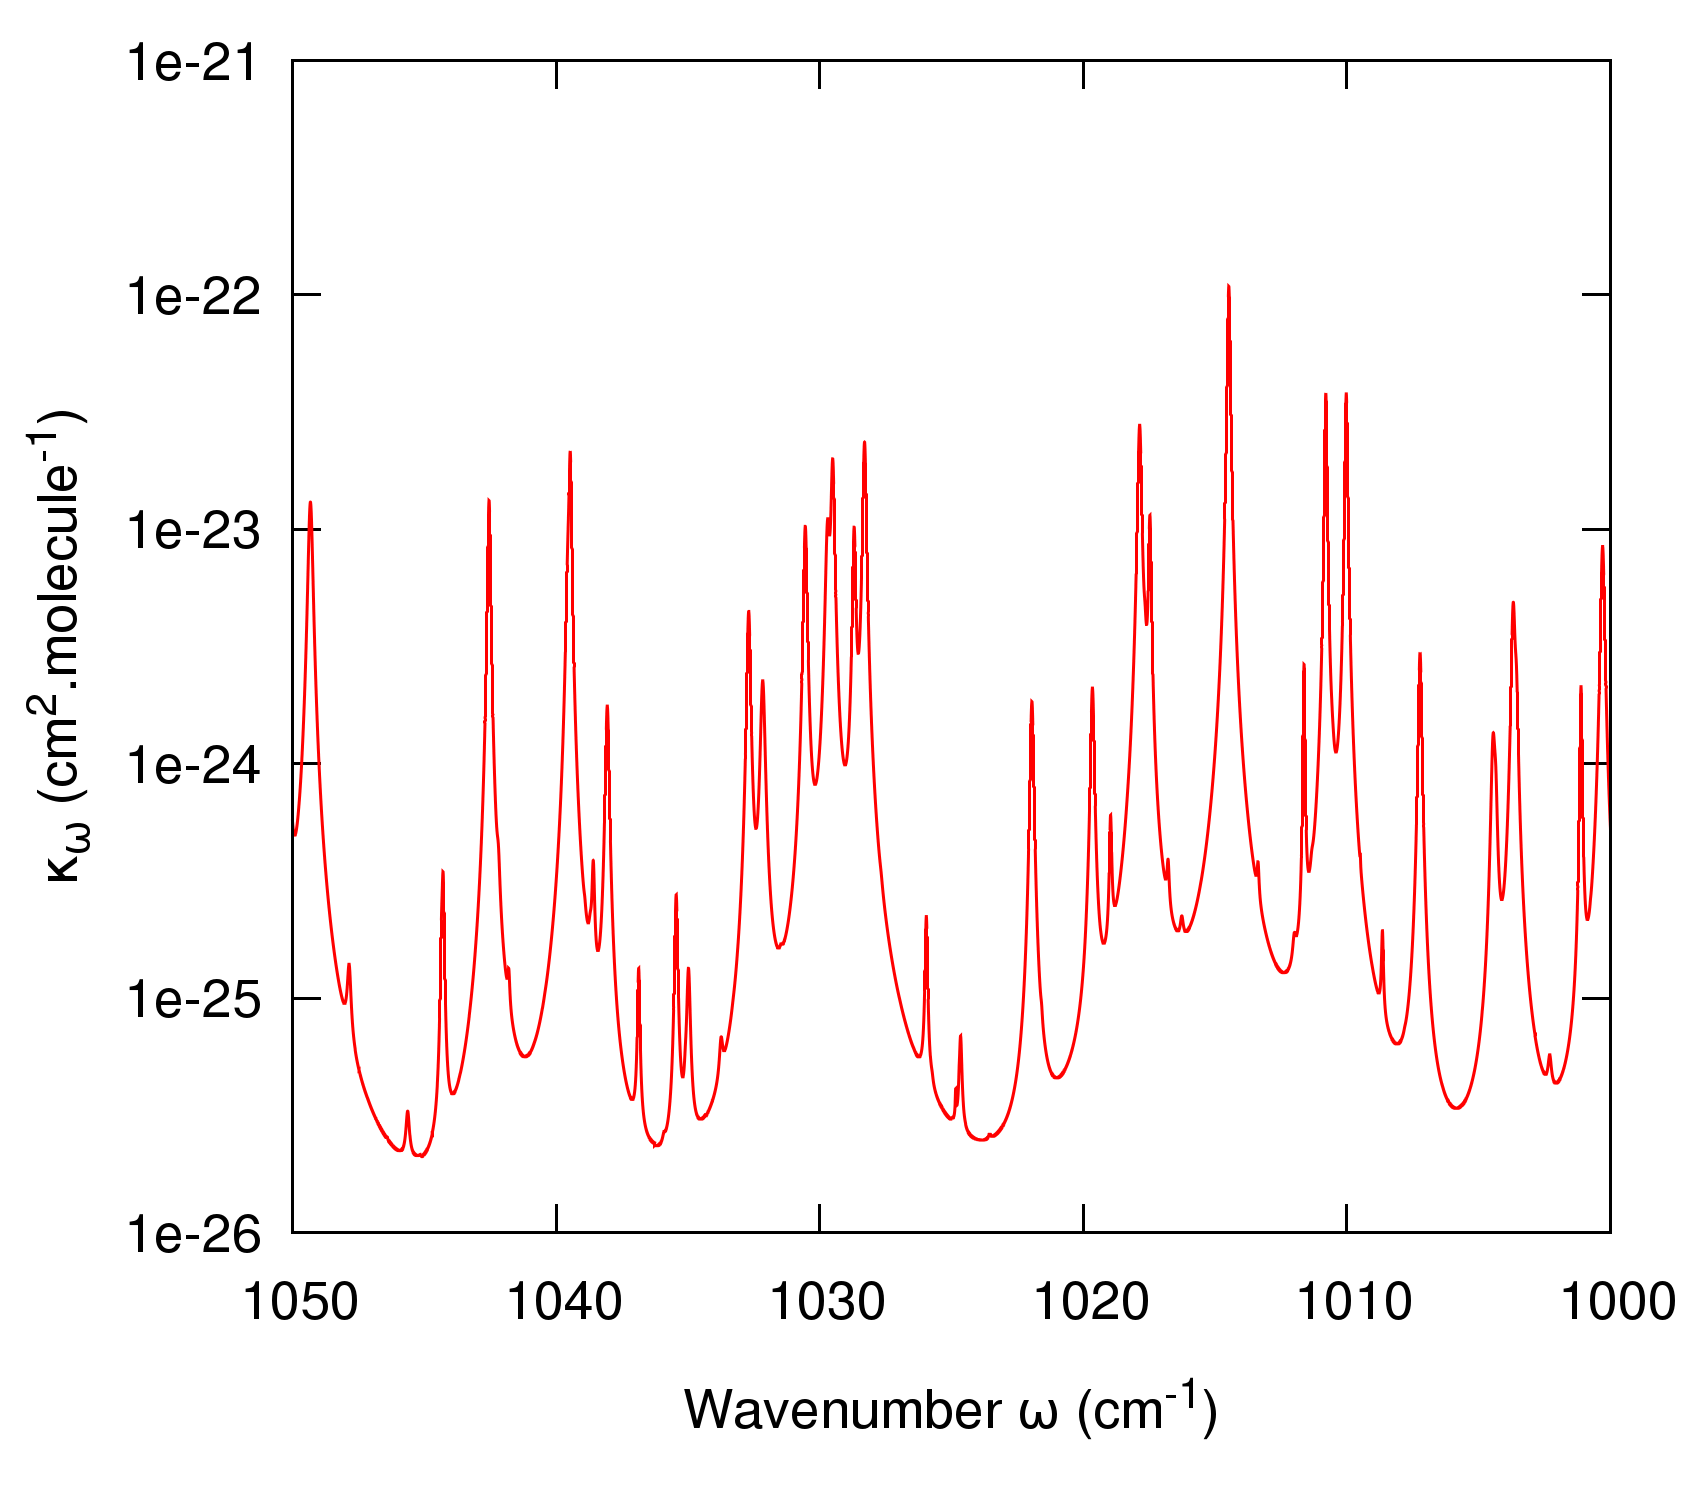
\includegraphics[width=4.0in]{Figures/H20_Line_Strength.png}
\end{center}
 \caption{Spectral $\rm H_2O$ absorption coefficient $\kappa_{\om}$ for the spectral range 1000 -- 1050~cm$^{\rm -1}$. This synthetic spectrum calculated using HITRAN 2012 line specifications assumes a temperature of 296~K and 10\% of water in a total pressure of 1~atm.\label{fig:H2O_Detailed_spectrum}}
\end{figure}

\subsection{Planck blackbody distribution law}

The Planck blackbody distribution law, sometime called the Planck function, but the term is misleading as it is a distribution, describes the spectral distribution of the equilibrium rate of radiant energy emitted from a blackbody at temperature $T$. Its expression is given, as a function of frequency $\nu$ and for an unit of solid angle, by:
\begin{equation}\label{eq:Plank_freqency}
I_{\rm b,\nu}(T) = \displaystyle\frac{2 h\nu^3}{c^2}\displaystyle\frac{1}{\exp\left(\displaystyle\frac{h\nu}{k_{\rm B}T}\right)-1}.
\end{equation}
Here, $h$ is the Planck constant ($6.626 \times 10^{-34}$~J$\cdot$s), and $k_{\rm B}$ is the Boltzmann constant ($1.381 \times 10^{-23}$~J/K). $I_{\rm b,\nu}(T)$ is in units of $\rm{W/m^{2}/str/s^{-1}}$.

In terms of wavenumber, the Planck blackbody distribution law, $I_{\rm b,\om}$, is written:
\be\label{eq:Planck_WN}
I_{\rm b,\om}(T) = \dfrac{2 \, h \, c^2 \, \om^{3}}{\exp\left(\dfrac{h \, c\, \om}{k_{\rm B} \, T }\right)-1} .
\ee
$I_{\rm b,\om}(T)$ is in units of $\rm{W/m^2/str/m^{-1}}$; the wavenumber $\om$ in Eq.~\ref{eq:Planck_WN} is in units of $\rm{m^{-1}}$.

The user who wishes to express the Planck blackbody distribution law as a function of wavelength should take caution when performing the change of variables. One should start by expressing that the radiant energy emitted at a wavelength $\la$ over an infinitesimal spectral range $\d\la$ is the same as the radiant energy emitted at the corresponding wavenumber $\om$ over an infinitesimal spectral range $\d\om$:
\be \label{eq:Planck_WN_WL}
I_{\rm b,\la}(T) \d \la = -I_{\rm b,\om}(T)\d \om,
\ee
the negative sign is introduced because $\om$ is the reciprocal of $\la$. Since $\la$ = 1/$\om$, it comes:
\be
\dfrac{\d \la}{\d \om} = -\dfrac{1}{\om^2}.
\ee
Equation \ref{eq:Planck_WN_WL} can be rewritten, after the appropriate change of variables:
\be \label{eq:Planck_WL}
I_{\rm b,\la}(T) = \dfrac{2 \, h \, c^2}{\la^5}\dfrac{1}{\exp\left(\dfrac{h \, c}{\la \, k_{\rm B} \, T }\right)-1},
\ee
where $I_{\rm b,\la}$ is in units of $\rm{W/m^2/str/m}$; the wavelength $\la$ in Eq.~\ref{eq:Planck_WL} is in unit of $\rm m$.

\begin{figure}
\begin{center}
 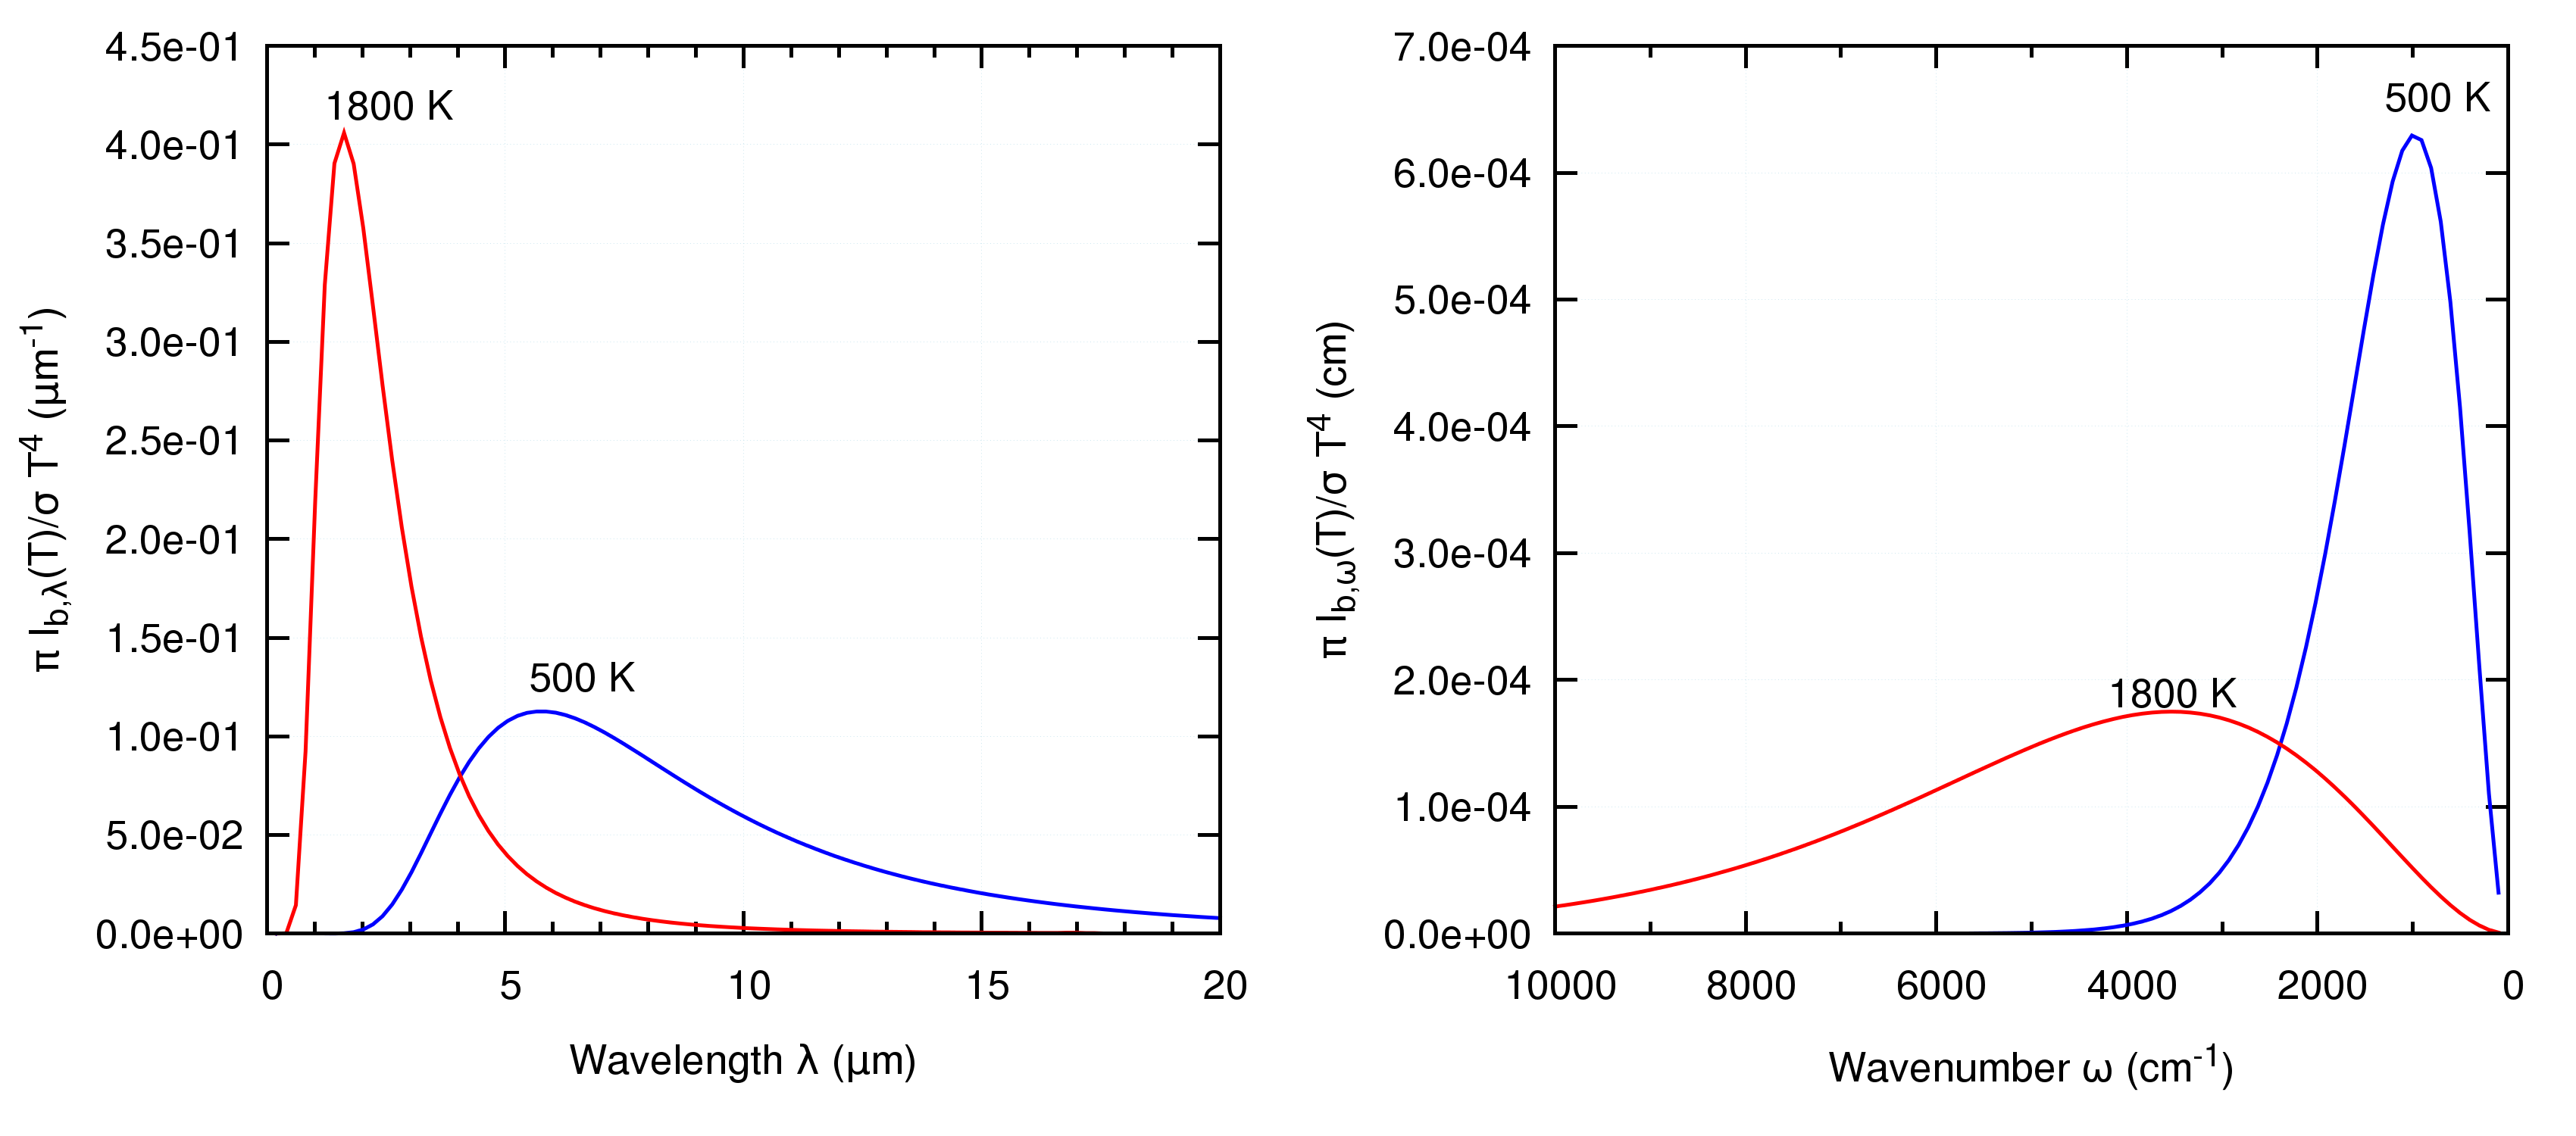
\includegraphics[width=6.5in]{Figures/Black_body.png}
\end{center}
 \caption{Normalized spectral Blackbody distributions at T = 500~K (blue line) and T = 1800~K (red line) with the wavelength in units of $\mu m$ (left) and with the wavenumber in units of $\rm cm^{-1}$ (right). \label{fig:bb_spectrum}}
\end{figure}

Figure~\ref{fig:bb_spectrum} plots profiles of normalized spectral Blackbody distribution for temperatures of 500~K and 1800~K using wavelength and wavenumber. It can be seen that an increase of temperature will shift the mode of the distribution toward lower wavelength and higher wavenumber. Figure~\ref{fig:bb_spectrum} indicates that the shape of the distribution is not invariant with the units chosen to characterize the spectrum. Indeed, while an elevation of blackbody temperature corresponds to a narrowing of the normalized distribution when using wavelength, the same elevation of blackbody temperature leads to a spreading of the profile when using wavelength. Finally, an important remark is that the location of the distribution mode (corresponding to the location of maximum emission) does not relate between wavelength and wavenumber. This location can be calculated using the Wien's displacement law. Using wavelength, the Wien's displacement law is expressed by:
\begin{equation}\label{eq:Wien_WL}
\la_{\rm max} T = 2898 \; \mu \rm m . \rm K,
\end{equation}
while using wavenumber, the Wien's displacement law is expressed by:
\begin{equation}\label{eq:Wien_WN}
 \dfrac{\om_{\rm max}}{T} = 1.961 \; \rm cm^{-1}.K^{-1}.
\end{equation}
Using Eq.~\ref{eq:Wien_WL}, the maximum of emission at 500~K is located at $\la_{\rm max} = \rm 5.8 \; \mu m$. The same calculation using Eq.~\ref{eq:Wien_WN} gives $\om_{\rm max} =  980 \; \rm cm^{-1}$. It is crucial to note that $10000/\la_{\rm max} = 1725 \; \rm cm^{-1} \; \neq \om_{\rm max}$. Hence caution must me taken when converting spectral variable from wavenumber to wavelength and vice versa. In RadCal, the wavenumber is the variable of choice for spectral quantities.

\section{Single line emission}
This section briefly recalls the characteristics of a single line emission. The expression for an isolated line with pressure broadening mechanism (also called Lorentz lines) is recalled along with the expression of lines broadened by Doppler effects. Note that RadCal mixes both lines expression in the calculation of the RTE. Hence, it is important to recall some of their properties. The underlying mechanisms responsible for the emission and/or absorption of electromagnetic radiation by a molecule or atom are not recalled here as they are out of the scope of this work. It is just recalled here that the discrete nature of a species spectrum in the infrared region is a direct consequence of the discretization of the vibrational and rotational energy level admissible for a given species. The location and intensity of these lines can be obtained from the solution of the time-dependent Schr\"{o}dinger wave equation of a molecule with an incident radiation field. The lines location and intensity depend on the molecule geometry, mass, and its electric dipole moments. For further details, see Chapter 7 of Penner, Ref.~\cite{Penner1959}; Herzberg Ref.~\cite{Herzberg1949}; Chapter 11 of Modest, Ref.~\cite{Modest2013}; and Tien monograph Ref.~\cite{Tien1968}.

\subsection{Lorentz lines}
A spectral line is never truly monochromatic as different line broadening mechanisms are present. The most fundamental one is the natural line broadening which is a consequence of the Heisenberg's uncertainty principle. While this effects is always present, it is usually omitted in engineering applications as the collision broadening and the Doppler broadening mechanisms are much more important.

The collision broadening mechanism originates from disruptions during the emission or absorption of energy due to the collision between molecules. The broadening of the line increases as the collision frequency increases, hence as the local pressure is increased. The shape of such broadened lines can be calculated using the electron theory of Lorentz or from quantum mechanism. The shape of the line is given by:
\begin{equation}\label{eq:lorentz_line}
 \kappa_{\om} = \dfrac{S}{\pi}\dfrac{\gamma_c}{\left( \om - \om_o\right)^2 + \gamma_c^2},
\end{equation}
where $\gamma_c$ is the collision broadening half-width at half the maximum (HWHM), $\omega_0$ is the wavenumber at the line center, and $S$ is called the line intensity or line strength and is defined as:
\begin{equation}
 S = \displaystyle\int{\kappa_{\om} \d \om}.
\end{equation}
Note that $S$ is a function of the temperature alone while $\gamma_c$ is a function of the temperature, pressure, and mixture composition. Because the effects of collision depend on the molecular diameters of the colliding species, the quantity $\gamma_c$ varies with the collisional partner. Among the collision broadening, distinction is made between the foreign gas broadening, \textit{i.e.} due to collisions among dissimilar species, and self-broadening, \textit{i.e} due to collisions among like species. The self-broadening collisions can be further differentiated between resonant and non-resonant collisions. Resonant collisions are more effective than non-resonant collisions but they have a different temperature dependence than non-resonant collisions. Non-resonant collisions are similar to collisions with a foreign gas. In RadCal, when not tabulated, the Lorentz HWHM $\gamma_{c,i}$ of a given species $i$ belonging to a mixture, is calculated according to:
\begin{equation}\label{eq:gamma_L}
 \gamma_{c,i} = \displaystyle\sum_{j} \gamma_{c0,(i,j)} \left(\dfrac{P_j}{P_0}\right)\displaystyle\sqrt{\dfrac{T_0}{T}} + \gamma^*_{c0,i}\dfrac{P_i}{P_0}\left(\dfrac{T_0}{T}\right),
\end{equation}
where $\gamma_{c0,(i,j)}$ denotes the value of non-resonant collision broadening HWHM with species $j$ at conditions of standard pressure (denoted $P_0$) and temperature (denoted $T_0$), and $\gamma^*_{c0,i}$ demotes the value of resonant self-collision broadening HWHM at conditions of standard pressure and temperature. Note that Eq.~\ref{eq:gamma_L} first right-hand side term includes the effects of foreign gas collision and non-resonant self-collision.

Profile of a normalized Lorentz line ($\kappa_{\omega} (\pi \gamma_c)/S$ as a function of $(\omega-\omega_0)/\gamma_c $) is plotted in Fig.~\ref{fig:Lorentz_line} together with the profile of a normalized Doppler line.

\begin{figure}
\begin{center}
 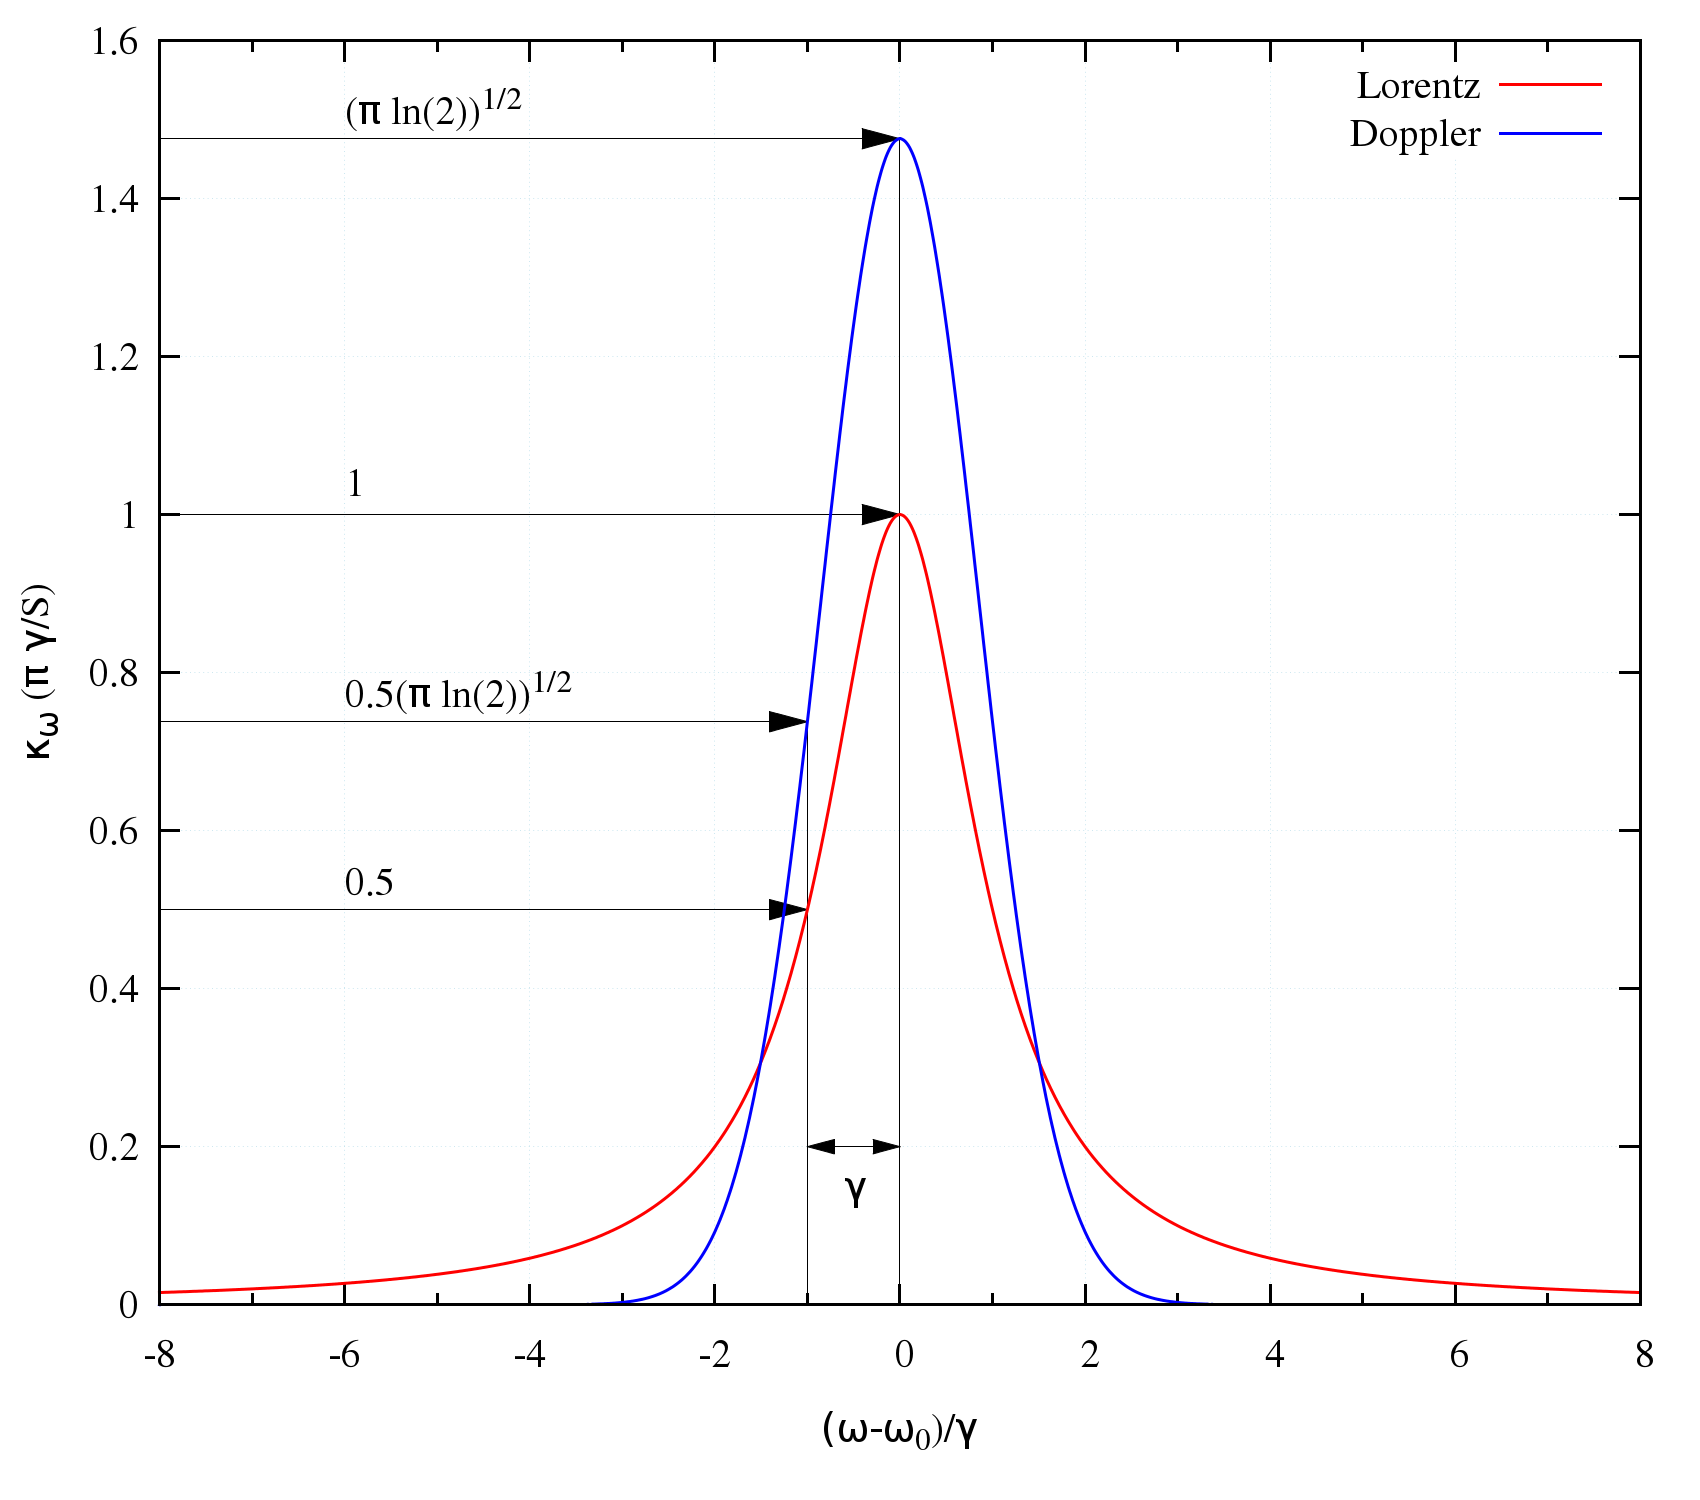
\includegraphics[width=4.0in]{Figures/Lorentz_Doppler.png}
\end{center}
 \caption{Profiles of a normalized Lorentz line (in red) and a normalized Doppler line (in blue). \label{fig:Lorentz_line}}
\end{figure}

\subsection{Doppler lines}
The motion of radiating particles in the line of sight may change the apparent frequency due to the Doppler effect. The apparent frequency increases when the particle moves toward the observer and decreases when it moves away. The Doppler line profile is calculated considering the Maxwell velocity distribution (which is a consequence of the local thermodynamic equilibrium assumption). The absorption coefficient is then expressed as:
\begin{equation}
\kappa_{\omega} = S \dfrac{\displaystyle\sqrt{\rm ln(2) }}{ \gamma_D \displaystyle\sqrt{\pi} } \exp{\left[- \rm ln(2) \left( \dfrac{\omega-\omega_0}{\gamma_D} \right)^2 \right]},
\end{equation}
where $S$ and $\omega_0$ are the line strength and the wavenumber at the line center, respectively. The quantity $\gamma_D$ is the Doppler HWHM. It is calculated from:
\begin{equation}\label{eq::DopplerHWHM}
  \gamma_D = \displaystyle\frac{\omega_0}{c} \displaystyle\sqrt{\rm{ ln(2)} \displaystyle\frac{2 k_B T}{m} },
\end{equation}
where $m$ is the mass of the radiating species. Note that the Doppler HWHM depends linearly on the wavenumber; it increases with elevated wavenumber.
The Doppler broadening mechanism is important at high temperature ($T > 2000\;K$) \cite{Modest2013} and/or low pressure, typically lower than 0.01 atm.
In RadCal both broadening mechanisms are included in the calculation of the RTE; see Section~\ref{sec:RTE_NB}.

\subsection{Emission from an isolated line}
This subsection recalls the results of the emission and absorption of radiation for an isolated Lorentz line. This ideal case helps to bring an understanding of a single line absorption variation with the pressure path length as it is a very fundamental concept.

The spectral variation of the absorption coefficient $\kappa_{\om}$ of a single line centered in $\om_0$, of line strength $S$, and of HWHM $\gamma_c$ with the wavenumber $\om$ is recalled:
\begin{equation}
 \kappa_{\om} = \dfrac{S}{\pi}\dfrac{\gamma_c}{\left( \om - \om_o\right)^2 + \gamma_c^2}. \tag{\ref{eq:lorentz_line}}
\end{equation}
The shape of the line is plotted in Fig.~\ref{fig:Lorentz_line}.

Assuming a path going through an isothermal gas, of temperature $T_g$, and homogeneous layer of participating species of partial pressure $P_i$, and of physical thickness $L$, the RTE, Eq.~\ref{eq:RTE_Final}, can be simplified as:
\begin{equation}
 I_{\om}(L) =  I_{\om}(0) \exp\left( -\kappa_{\om} P_i L\right) + I_{\rm b,\om}\left(T_g\right) \left(1-\exp\left(-\kappa_{\om} P_i L\right)\right).
\end{equation}
Note that in this equation, the local amount of participating species is expressed by the partial pressure $P_i$; hence in the equation above, $\kappa_{\om}$ has the dimension of an inverse pressure times an inverse length. In RadCal, $\kappa_{\om}$ is expressed in $\rm (cm^{-1} \cdot atm^{-1})$, while $P_i$ is in $\rm atm$ and the path physical length $L$ is in $\rm cm$. The product $P_i\;L$, the pressure path length, is referred to in RadCal as a species optical thickness and is also denoted $U$, and the product $\kappa_{\om}\;P_i\;L$ is referred to as the optical depth.

Considering only the emission term (\textit{i.e.} $I_{\om}(0)$ = 0), the exiting intensity integrated over the whole spectrum, emitted by a single line, denoted $I(L)$, is expressed as:
\begin{equation}
I(L) =  I_{\rm b,\om}\left(T_g\right) \displaystyle\int_{\Delta \om}\left( 1-\exp\left(-\kappa_{\om'} P_i L\right)\d \om'\right),
\end{equation}
this assumes that $I_{\rm b,\om}$ does not vary much over the $\Delta \om$ range. The integrand is often called the equivalent line width \cite{Modest2013} and is usually denoted $W$,
\be
W = \displaystyle\int_{\Delta \om}\left( 1-\exp\left(-\kappa_{\om'} P_i L\right)\d \om'\right).
\ee

The analytical expression of $W$ for a Lorentz line can be derived, see for example Penner, \cite{Penner1959}:
\be
W(P_i L) = 2 \pi \gamma_c L(x) = 2  \pi \gamma_c x \;\exp\left( -x\right) \left(I_0(x) + I_1(x)\right), \; x = \dfrac{SP_iL}{2 \pi \;\gamma_c}.
\ee
The function $L(x)$ is named the Ladenburg-Reiche function, and $I_0$ and $I_1$ are the modified Bessel functions of the first kind. The graph of the Ladenburg-Reiche function is
given in Fig.~\ref{fig:Ladenburg}. Note that for small and large values of $x$, the equivalent line has the following asymptotic forms:
\begin{align}
W(x) \sim SP_iL ,\: {\rm for}\: x \ll 1 \\
W(x) \sim 2\sqrt{S\gamma_c P_iL} ,\: {\rm for}\: x \gg 1.
\end{align}

\begin{figure}
\begin{center}
 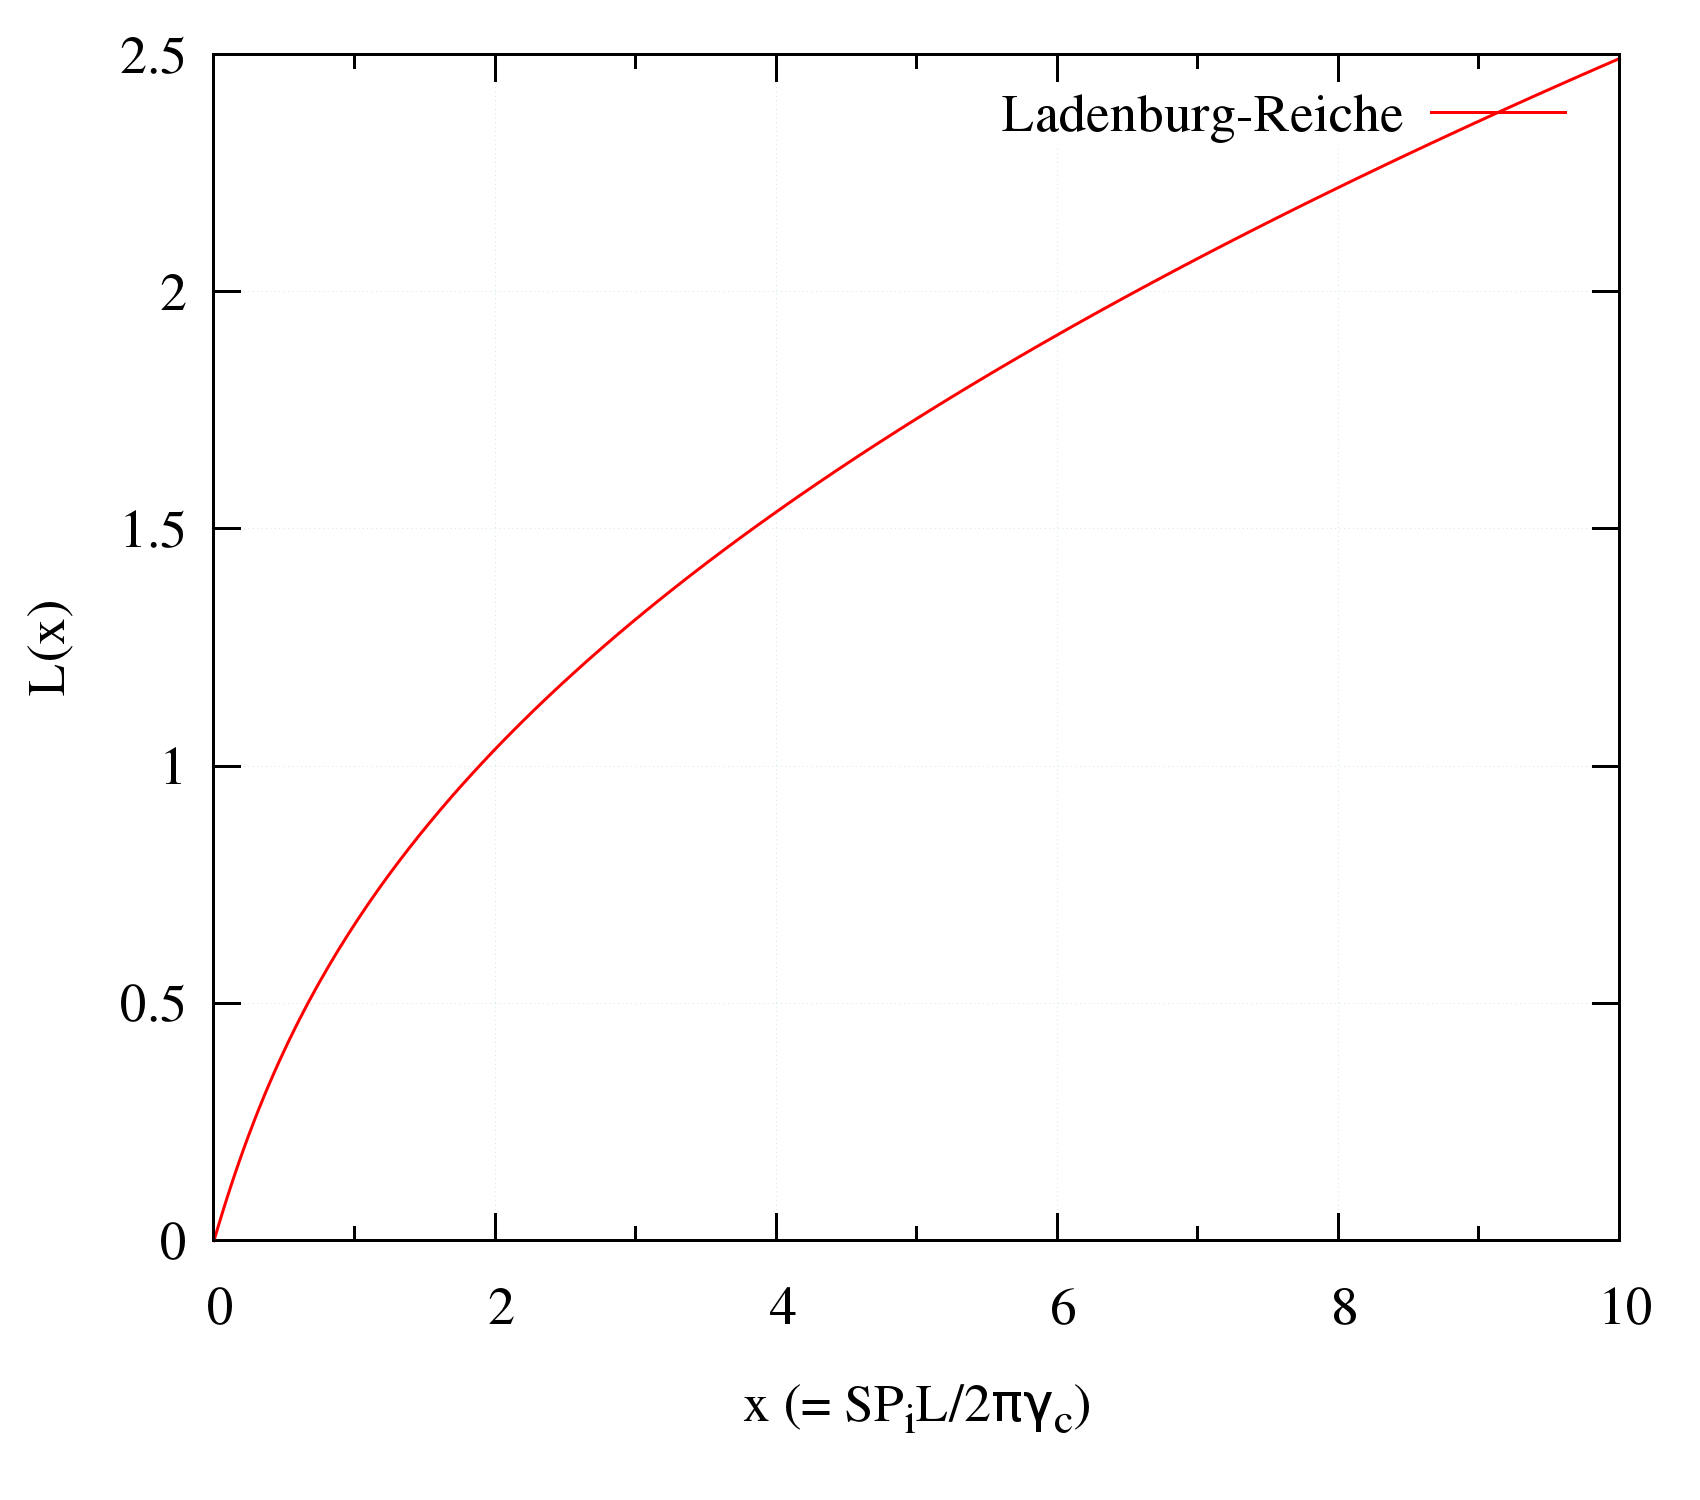
\includegraphics[width=4.0in]{Figures/Ladenburg.png}
\end{center}
 \caption{Profile the Ladenburg-Reiche function. \label{fig:Ladenburg}}
\end{figure}

It is worth noting that the parameter $x$ gives an indication of the optical thickness of the gas layer for a single line. When $x$ is small, this indicates that the medium is weakly participating (either $S$ or the product $P_iL$ is small) and the absorption and emission of a single line is linear with the product $P_iL$. On the contrary, when $x$ is much greater than unity, the absorption or emission of a single line is not linear anymore but has a square-root dependency.

\section{Narrow band models}\label{Sec::SNBM}
This section briefly describes the different models used to obtain most of the tabulated species IR spectral mean absorption coefficients at different temperatures, $\bar{\kappa}_i(\om,T)$. Narrow band models are used in lieu of line-by-line models to represent the IR spectra of radiating species in engineering applications. In the narrow-band approach, the whole spectrum is divided into small spectral bands (typically several $\rm cm^{-1}$), and different statistical approaches are used to compute the average radiative properties over these narrow-bands. What is of interest is to give functional expression of the integrand:
\be
\bar{\tau}_{\om} = \displaystyle\int_{\Delta \om}\left( \exp\left(-\kappa_{\om'} P_i L\right)\d \om'\right),
\ee
when $\Delta \om$ is large enough so it includes hundreds, even thousands, of single lines, but small enough to assume $I_{\rm b,\om}\left(T_g\right)$ and the incident spectral intensity $I_{\om}(0)$ constant over it. It is important to state that generally:
\be
\bar{\tau}_{\om} \neq \displaystyle\int_{\Delta \om}\left( \exp\left(-\bar{\kappa}_{\om'} P_i L\right)\d \om'\right).
\ee
Equality is verified only is some specific situations (\textit{e.g.} $P_iL \ll 1$). An important assumption to recall is that it is assumed that the Kirchoff law, \textit{i.e.} $\bar{\alpha} = \bar{\epsilon}$, holds over a narrow-band.

Three main narrow-band models are presented below: the Elsasser model, the Goody model, and the Malkmus model. All assume Lorentz lines.

\subsection{Elsasser model}

The Elsasser model assumes all the lines to have the same HWHM $\gamma_c$, the same line strength $S$, and to be equally spaced every $d$ wavenumber from each other.
As a consequence, the absorption coefficient can be expressed by the infinite sequence:
\be\label{eq:kappa_El}
\kappa_{\om} = \displaystyle\sum_{n = -\infty}^{\infty}{\dfrac{S}{\pi}\dfrac{\gamma_c}{\left(\om - \left(\om_0+n\,d\right)\right)^2 + \gamma_c^2}}.
\ee
This function is periodic, with a period $d$. Following Elsasser derivation (see Ref.~\cite{Penner1959}), Eq.~\ref{eq:kappa_El} can be expressed as:
\be\label{eq:Elsasser_periodic}
\kappa_{\om}  = \dfrac{S}{d} \dfrac{\rm sinh (8\beta)}{{\rm cosh (8\beta)} - \cos(\frac{2\pi}{d}(\om-\om_0))},
\ee
where the overlap parameter $\beta$, which is also called the (Lorentz) fine structure parameter and denoted $a_c$ in Ref.~\cite{Ludwig1973} and in the code, is defined here as:
\be\label{eq::beta}
\beta = \dfrac{\pi}{4}\dfrac{\gamma_c}{d}.
\ee
The mean absorption coefficient $\bar{\kappa}$ over the narrow-band centered in $\om$ is:
\be\label{eq:kappa_def}
\bar{\kappa}_{\om} = \dfrac{S}{d}.
\ee
Figure~\ref{fig:Elsasser_profile} plots the variations of the Elsasser absorption coefficient $\kappa_{\om}$ normalized by $\bar{\kappa}$ as a function of the ratio $\om/d$ for two different values of the overlap parameter $\beta$. Strong overlap effects are seen for the largest value of $\beta$.

\begin{figure}
\begin{center}
 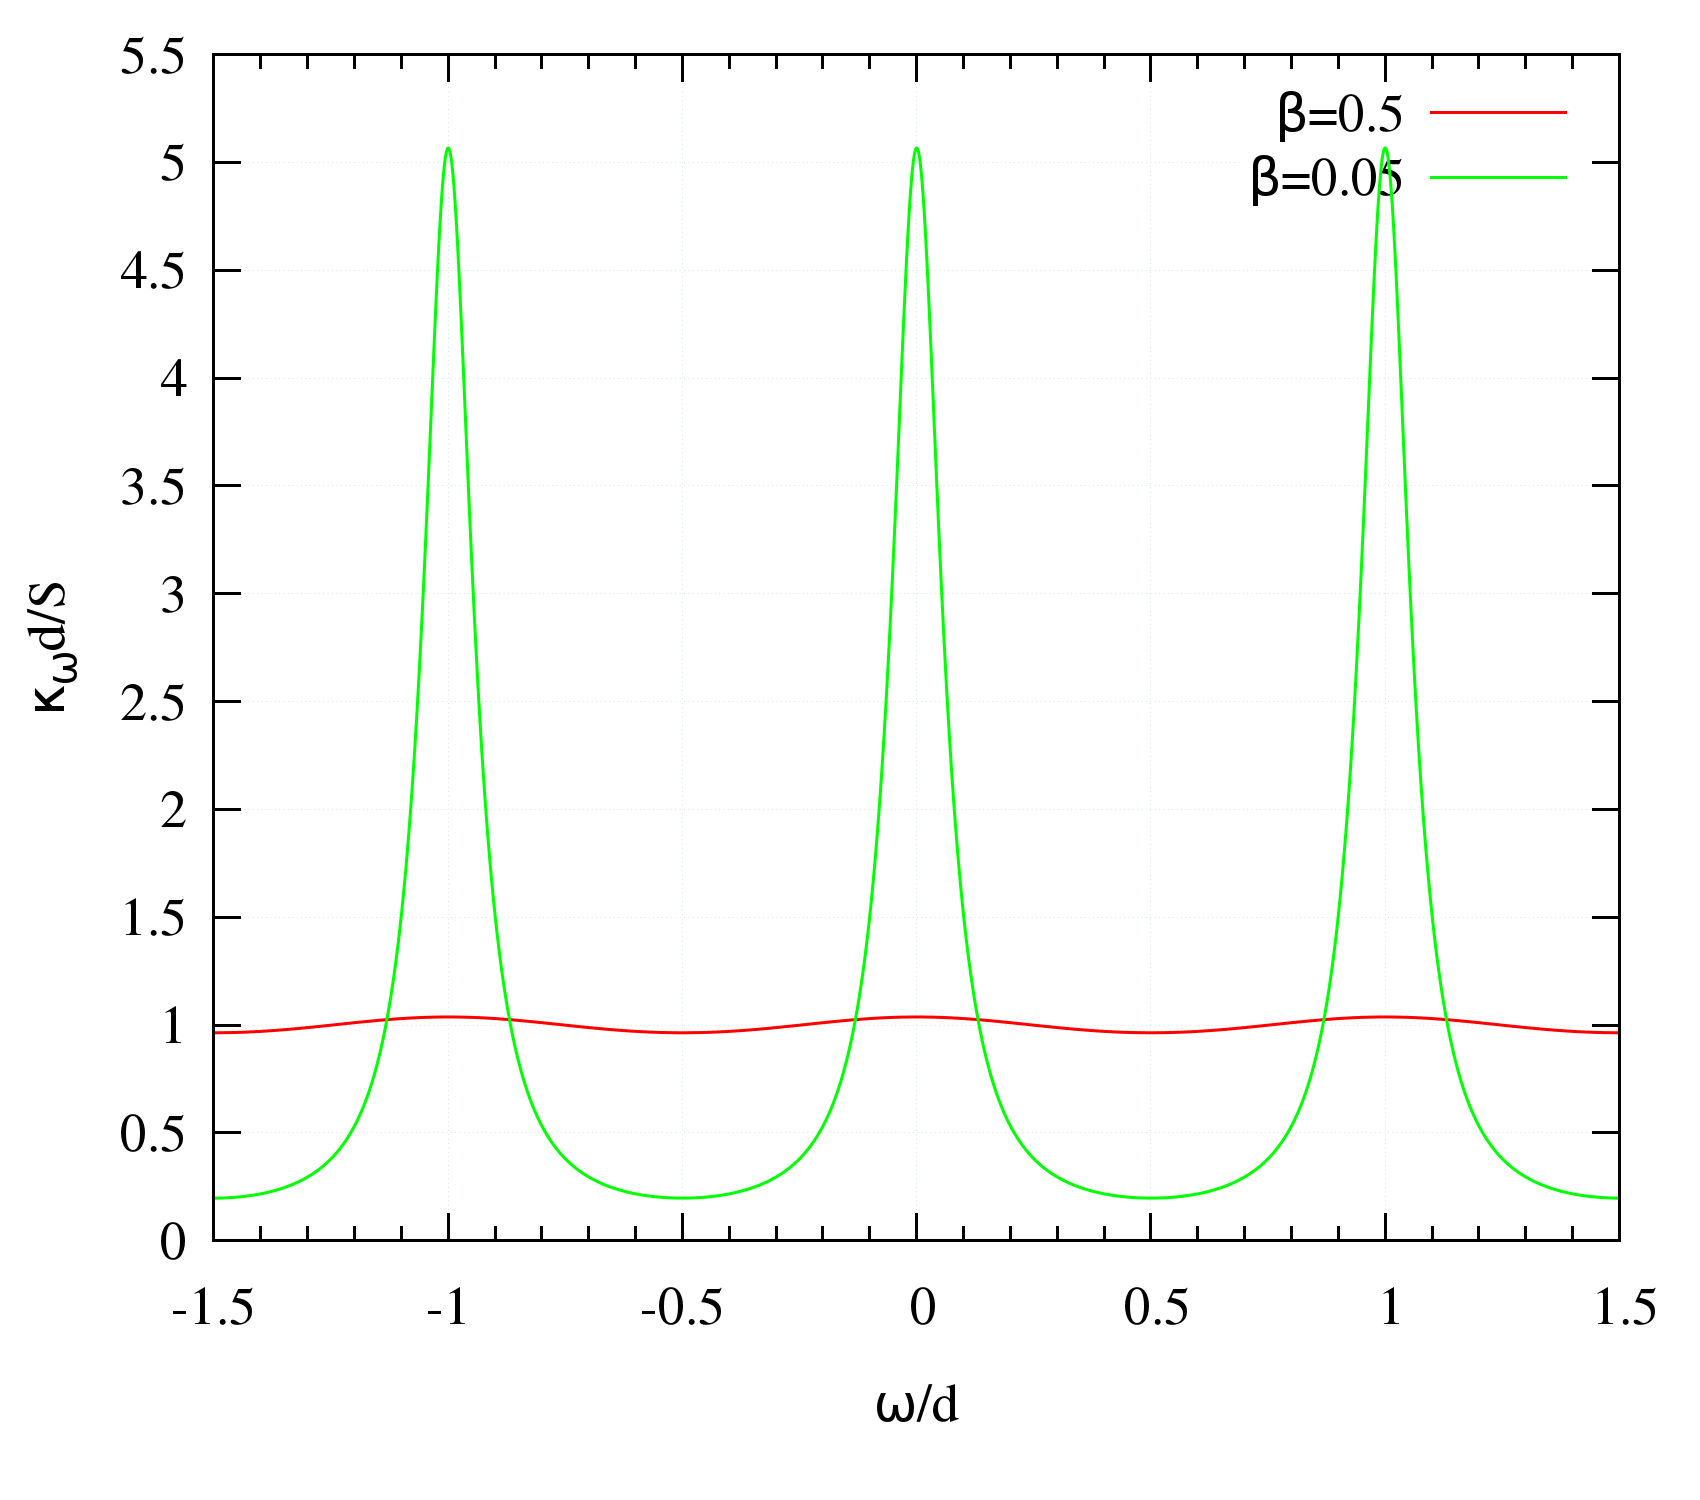
\includegraphics[width=4.0in]{Figures/Elsasser_profile.png}
\end{center}
 \caption{Variations of the Elsasser absorption coefficient normalized by $\bar{\kappa}$ plotted as a function of the ratio $\om/d$ for two different values of the overlap parameter $\beta = 0.05$ (in green) and $\beta = 0.5$ (in red). \label{fig:Elsasser_profile}}
\end{figure}
The mean transmissivity $\bar{\tau}_{\om}$ of the narrow-band centered in $\om$ can be calculated using Eq.~\ref{eq:Elsasser_periodic}, averaging over one period $d$:
\be
\bar{\tau}_{\om} = \frac{1}{d}\displaystyle\int_{-\frac{d}{2}}^{\frac{d}{2}}{\exp\left(-\bar{\kappa}_{\om} P_i L\dfrac{\rm sinh (8\beta)}{{\rm cosh (8\beta)} - \cos\left(\frac{2\pi}{d}(\om'-\om)\right)} \right)\d\om'}.
\ee
This expression can be assessed using the Godson and Tien approximations \cite{Brosmer1985b,Kunitomo1975}:
\be\label{eq::Elsasser}
    \bar{\tau}_{\om} = 1- \erf \left( \dfrac{\sqrt{\pi}}{2} \, \frac{\bar{\kappa}_{\om} \, U }{\displaystyle \sqrt{1 + \frac{\pi \, \bar{\kappa}_{\om} \, U}{16 \, \beta}}}  \right),
\ee
where $U = P_iL$ is the optical thickness. Equation~\ref{eq::Elsasser} is used in RadCal to compute $\bar{\tau}_{\om}$ when using the Elsasser narrow-band model, which is only used for Methane. Note that the Godson and Tien approximation is reasonably accurate for values of the overlap parameter lower or of the order of unity, \textit{i.e.} $\beta < 1$.
Figure~\ref{fig::Elsasser_curve_growth} plots the quantity $-\ln(\bar{\tau}_{\om})$ (this quantity is also referred to as the curved of growth) versus the product $\bar{\kappa}_{\om} U$ for two different values of the overlap parameter: $\beta = 0.05$ (in green) and $\beta = 0.5$ (in red). The back dashed curve corresponds to the ``linear'' behavior, \textit{i.e.} $\bar{\tau}_{\om} = \exp\left(\bar{\kappa} U\right)$. It is noteworthy that this linear behavior corresponds to either ``weak lines regimes'' (situations with small product $\bar{\kappa} U$) or to situations with a strong overlap, $\beta > 1$). Outside of these regimes, assuming linear behavior might lead to overestimation of the curve of growth. Figure~\ref{fig::Elsasser_curve_growth} also illustrates a case where the Godson and Tien approximation looses its accuracy and leads to unphysical results, as seen for the case $\beta=0.5$, which overestimates the absorption.

It can be seen from Eq.~\ref{eq::Elsasser} that $\bar{\tau}_{\om}$ is fully characterized once the narrow-band parameters $\bar{\kappa}_{\om}$ and $\beta$ are known. Note that these two parameters are by construction independent of the physical length of radiation propagation but depend on the local temperature, pressure, and local mixture composition.

\begin{figure}
\begin{center}
 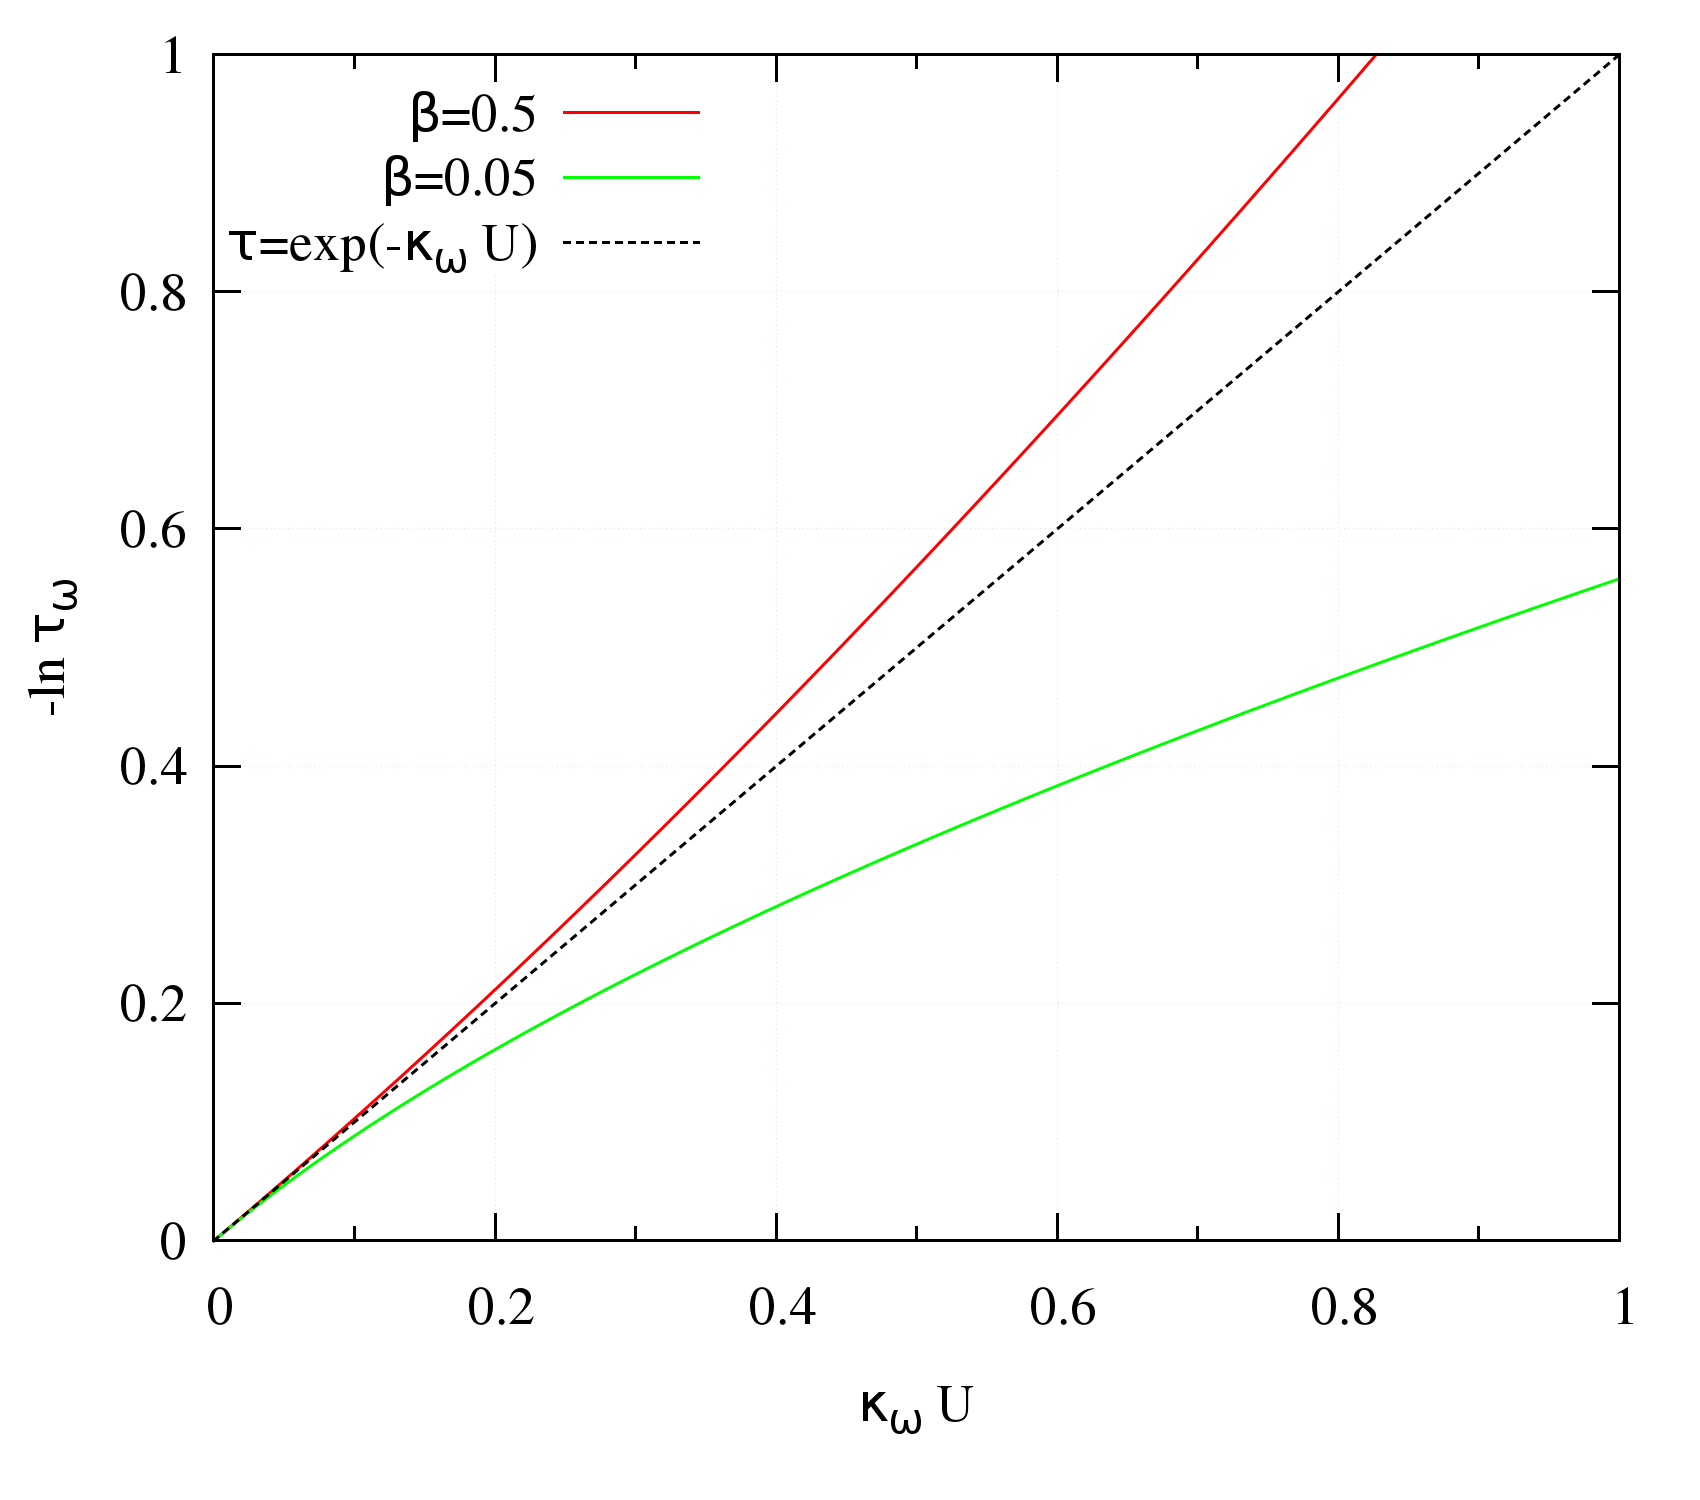
\includegraphics[width=4.0in]{Figures/Elsasser_curve_of_growth.png}
\end{center}
 \caption{Elsasser model curve of growth ($\ln \bar{\tau}$) as a function of the product $\bar{\kappa}_{\om} U$. Two different values of the overlap parameter are plotted: $\beta = 0.05$ (in green) and $\beta = 0.5$ (in red). The curve of growth for the ``weak line regime'' is plotted in the bash dashed curve.\label{fig::Elsasser_curve_growth}}
\end{figure}

\subsection{Generalities on statistical narrow-band models}
The Goody and Malkmus models have been developed to provide a better modeling of the narrow-band spectral properties than that predicted by the Elsasser model, which is based on strong assumptions: uniformity of the line strength and of line spacing. While the Elsasser model works fine for some light, diatomic  species (\textit{i.e} HCl), most of the more complex polyatomic species cannot be modeled appropriately with the Elsasser model, since the very detailed experimental characterization of their spectral lines does not exhibit regularity \cite{Modest2013}.

The Goody and Malkmus models are statistical narrow-band models, the former preceding the latter by a couple of decades and was first developed by Mayer and Goody \cite{Penner1959}. Statistical narrow-band models are based on two main assumptions: first, there is no correlation between lines position and line intensities, and the location of the line can be modeled by any random arrangement~\cite{Penner1959,Young1977d}; second, while all the lines have the same shape, their line strength within the narrow-band of spectral range $\Delta \nu$ is a random variable assigned to a continuous probability density function $P(\bar{S},S)$, with $\bar{S}$ the mean value of the line strength, \textit{i.e.} $\bar{S} = \displaystyle\int_{0}^{+\infty}{S P(\bar{S},S)\d S}$.

A consequence of these assumptions for a very large number of lines contained within the narrow-band is that the transmissivity of a narrow-band $\bar{\tau}_{\om}$, and of optical thickness $U$, is expressed by:
\be\label{eq:SNB_tau_equiline}
\bar{\tau}_{\om}(U) = \exp\left(-\displaystyle\frac{\bar{W}(U)}{d}\right),
\ee
where $d$ is the average line spacing and $\bar{W}(U)$ is the average equivalent line width of the narrow-band considered and is calculated as:
\begin{align}\label{eq::SNB_Equiline}
\bar{W}(U) &= \displaystyle\int_{0}^{+\infty}{P(\bar{S},S)W(S,U) \d S} \nonumber \\
           &= \displaystyle\int_{0}^{+\infty}{P(\bar{S},S)\displaystyle\int_{-\infty}^{+\infty}{1 - \exp\left(-\kappa_{\om} P_i L\right) \d\om} \d S}
\end{align}
where $\kappa_{\om}$ is the absorption coefficient of a Lorentz line, given by Eq.~\ref{eq:lorentz_line}. An example of the derivation of Eq.~\ref{eq::SNB_Equiline} is presented in Penner's book~\cite{Penner1959}. By their different choice of the probability density function $P(\bar{S},S)$, the Goody and Malkmus models provide an explicit and simple evaluation of the average equivalent line width of a narrow-band, $\dfrac{\bar{W}}{d}$.

\subsection{Goody model}\label{sec:goody_model}

The Goody model assumes an exponential distribution of the line strength:
\begin{align}
 P(\bar{S},S) &= \dfrac{1}{\bar{S}}\exp\left(-\dfrac{S}{\bar{S}} \right) \\
              &= \dfrac{4}{\pi S_E}\exp\left(-\dfrac{4S}{\pi S_E} \right),
\end{align}
where $S_E$ is an effective equivalent line strength which relates to the average line strength $\bar{S}$ with \cite{Malkmus1967,Ludwig1973}:
\be\label{eq::S_E_barS}
\bar{S} = \dfrac{\pi}{4} S_E.
\ee
Solving Eq.~\ref{eq:SNB_tau_equiline} and introducing the effective average lines spacing $d_E = \dfrac{4}{\pi}d$, Ref.~\cite{Malkmus1967}, it comes:
\begin{align}\label{eq::Goody}
    \bar{\tau}_{\om} = \exp\left(-\dfrac{S_E}{d_E} \dfrac{U}{\displaystyle \sqrt{1+\frac{S_E U}{4 \, \gamma_c }}}\right) \nonumber \\
    \bar{\tau}_{\om} = \exp\left(-\frac{\bar{\kappa}_{\om} \, U} {\displaystyle \sqrt{1+\frac{\bar{\kappa}_{\om} \, U}{4 \, \beta}}}\right)
\end{align}
where the band overlap parameter $\beta$ is here defined as:
\be
\beta = \dfrac{\gamma}{d_E} = \dfrac{\pi}{4}\dfrac{\gamma}{d}.
\ee
It is important to remark that the band overlap parameter $\beta$, while constant over a narrow-band, varies with the wavenumber. In addition, it has a strong dependence on the total pressure. This dependence varies from species to species. The mean absorption coefficient $\bar{\kappa}$ in Eq.~\ref{eq::Goody} keeps the same definition as given in Eq.~\ref{eq:kappa_def}. It is noteworthy to realize that:
\be
\bar{\kappa} = \dfrac{S}{d} = \dfrac{S_E}{d_E},
\ee
from the definition of $d_E$ and $S_E$. The effective parameter has been introduced to be consistent with the definition from Ludwig \textit{et al.}, Ref.~\cite{Ludwig1973}, from which most of RadCal is formulated after.

Figure~\ref{fig::Goody_curve_growth} plots the curve of growth, $-\ln(\bar{\tau}_{\om})$, versus the product $\bar{\kappa}_{\om} U$ for two different values of the overlap parameter: $\beta = 0.05$ (in green) and $\beta = 0.5$ (in red) using the Goody model. The back dashed curve corresponds to the ``linear'' behavior, \textit{i.e.} $\bar{\tau}_{\om} = \exp\left(\bar{\kappa} U\right)$.

Again, it can be seen from Eq.~\ref{eq::Goody} that $\bar{\tau}_{\om}$ is fully characterized once the narrow-band parameters $\bar{\kappa}_{\om}$ and $\beta$ are known.

\begin{figure}
\begin{center}
 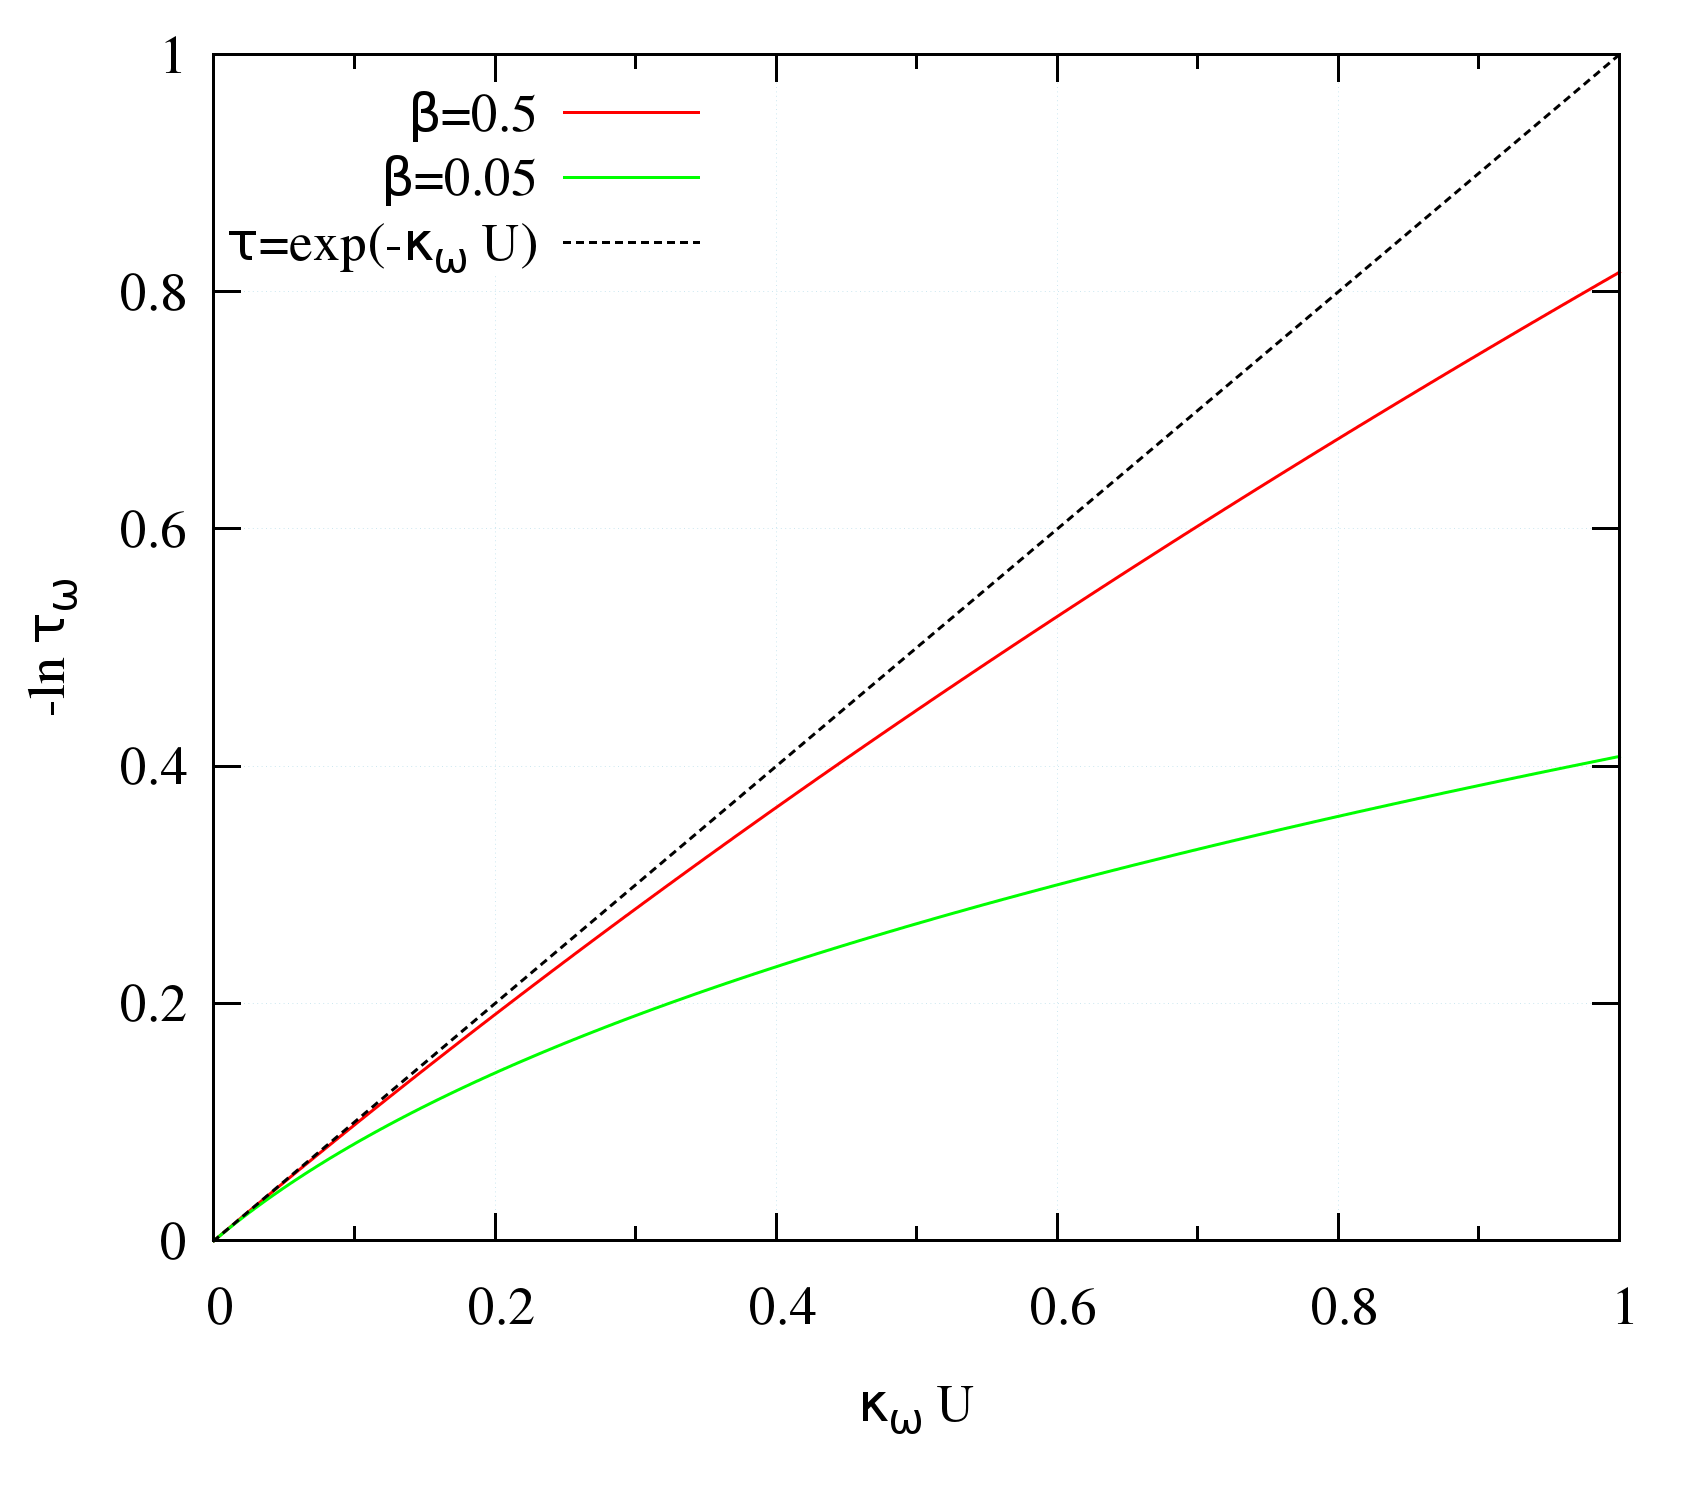
\includegraphics[width=4.0in]{Figures/Goody_curve_of_growth.png}
\end{center}
 \caption{Goody model curve of growth ($\ln \bar{\tau}$) as a function of the product $\bar{\kappa}_{\om}\;U$. Two different values of the overlap parameter are plotted: $\beta = 0.05$ (in green) and $\beta = 0.5$ (in red). The curve of growth for the ``weak line regime'' is also plotted (dashed curve).\label{fig::Goody_curve_growth}}
\end{figure}

\subsection{Malkmus model}\label{sec:malkmus_model}

Like the Goody model, the Malkmus model assumes the line strength of all the lines in a given narrow-band model follows a particular distribution. This model was developed because the exponential distribution assumed in the Goody model substantially underestimates the number of low-intensity lines. The Malkmus model is based on a more physical approach that assumes that the line strength distribution $P(S)$ varies proportionally to $S^{-1}$. This assumption is based on physical arguments and is empirically verified for some molecules, see Malkmus~\cite{Malkmus1967} for more details.

The problem of non-normalization of the $S^{-1}$ distribution is circumvented by cutting-off the $S^{-1}$ distribution below some very small and above some very large values of $S$. A continuous distribution can then be constructed based on some assumptions relating the energy of a transition with the line strength and assuming that the ratio between the maximum and the minimum line strengths considered is very large. The line strength probability distribution used in the Malkmus model is expressed by an exponential-tailed $S^{-1}$ distribution \cite{Malkmus1967,Young1977d}:
\begin{equation}
 P(S_E,S) = \dfrac{1}{S}\exp\left(-\dfrac{4}{\pi}\dfrac{S}{S_E} \right),
\end{equation}
where the effective line strength $S_E$ relates to the average line strength $\bar{S}$ through Eq.~\ref{eq::S_E_barS}. Solving Eq.~\ref{eq:SNB_tau_equiline}, and using the same definition for the effective average lines spacing $d_E$ as given in the above section, it comes:
\begin{align}\label{eq::Malkmus}
    \bar{\tau}_{\om} = \exp\left( -2 \dfrac{\gamma_c}{d_E} {\displaystyle \sqrt{1+\frac{S_E U}{\gamma_c }} -1 }\right) \nonumber \\
    \bar{\tau}_{\om} =  \exp\left(-2  \beta \left[\sqrt{1+\dfrac{\bar{\kappa}_{\omega}U}{\beta} }- 1\right] \right)
\end{align}
where the band overlap parameter $\beta$ is here again defined as:
\be
\beta = \dfrac{\gamma}{d_E} = \dfrac{\pi}{4}\dfrac{\gamma}{d}.
\ee

The Malkmus band model is recognized as the most suitable statistical narrow-band model for polyatomic gases \cite{Modest2013}. In this new version of RadCal, this model has been introduced to model the newly implemented fuel species. Note that the Malkmus and Goody models do not differ when considering the extreme cases of optically thin and optically thick medium. In such cases, both models asymptote to:
\begin{align}
\lim_{U \to 0} \dfrac{\bar{W}}{d}/U &= \bar{\kappa} \\
\lim_{U \to +\infty} \dfrac{\bar{W}}{d}/\sqrt{U} &= 2\displaystyle\sqrt{\bar{\kappa}\beta}
\end{align}

Figure~\ref{fig::Malkmus_curve_growth} plots the curve of growth, $-\ln(\bar{\tau}_{\om})$, versus the product $\bar{\kappa}_{\om} U$ for two different values of the overlap parameter: $\beta = 0.05$ (in green) and $\beta = 0.5$ (in red) using the Malkmus model. The back dashed curve corresponds to the ``linear'' behavior, \textit{i.e.} $\bar{\tau}_{\om} = \exp\left(-\bar{\kappa} U\right)$.

Again, it can be seen from Eq.~\ref{eq::Malkmus} that $\bar{\tau}_{\om}$ is fully characterized once the narrow-band parameters $\bar{\kappa}_{\om}$ and $\beta$ are known. These two narrow-band spectral quantities can be obtained either from line-by-line calculations, by fitting experimental data, or by physical considerations.

\begin{figure}
\begin{center}
 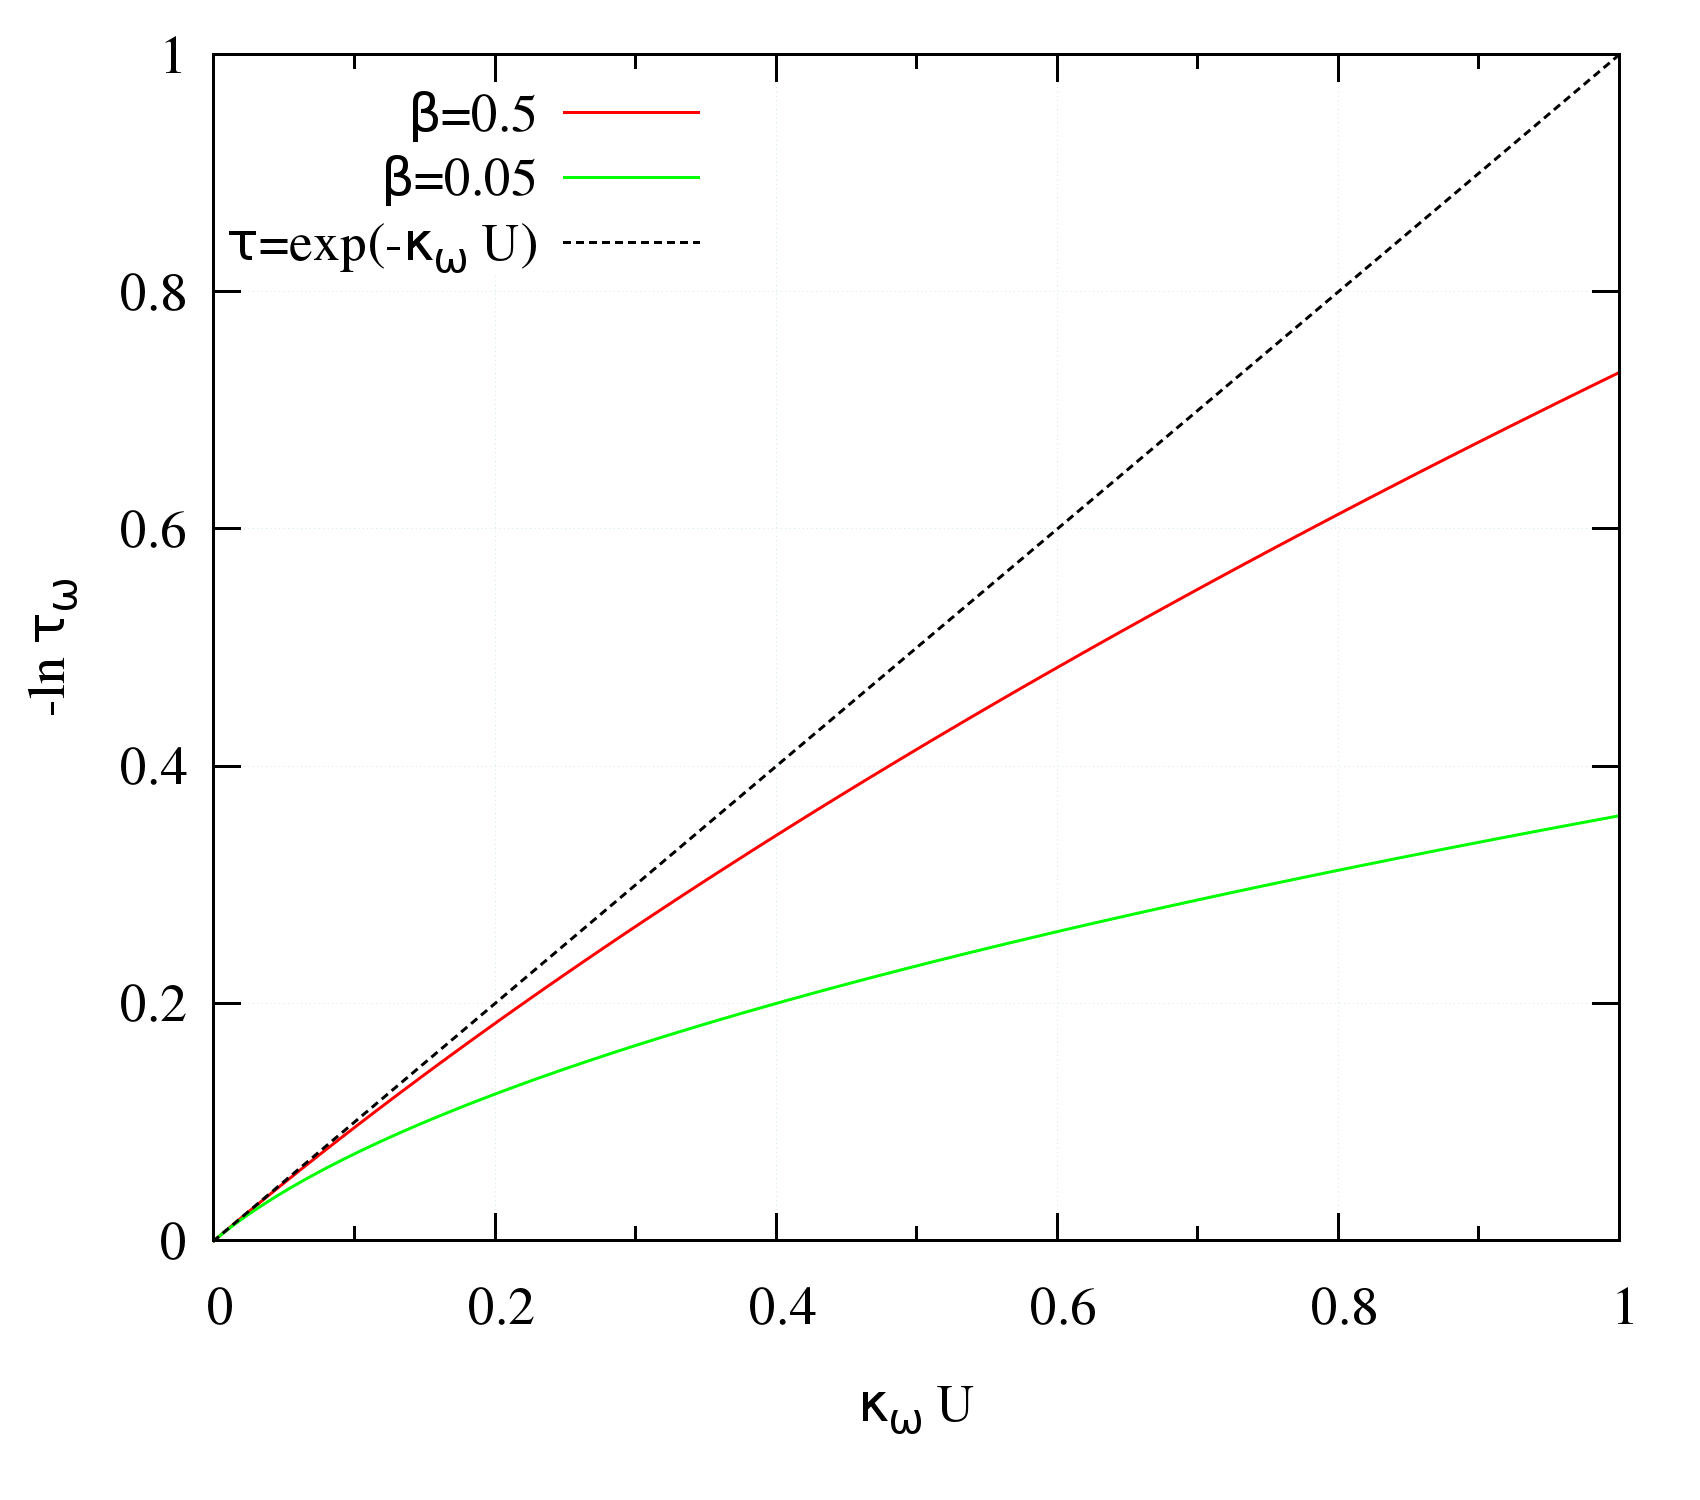
\includegraphics[width=4.0in]{Figures/Malkmus_curve_of_growth.png}
\end{center}
 \caption{Malkmus model curve of growth ($-\ln \bar{\tau}$) as a function of the product $\bar{\kappa}_{\om} U$. Two different values of the overlap parameter are plotted: $\beta = 0.05$ (in green) and $\beta = 0.5$ (in red). The curve of growth for the ``weak line regime'' is also plotted (dashed curve).\label{fig::Malkmus_curve_growth}}
\end{figure}

\textbf{Note}: For all the tabulated data, a linear interpolation of $\bar{\kappa}_{\om}$ and $\beta_{\om}$ in temperature and/or in wavenumber is performed by RadCal when necessary. If the temperature sought is out of the tabulated data range, then the data at the nearest temperature are used.

\section{Treatment of the RTE in the scope of narrow-band model}\label{sec:RTE_NB}
This section presents the expression of the different calculations performed by RadCal to numerically solve the Radiative Transfer Equation for a narrow-band. The Radiative Transfer Equation for a narrow-band is recalled below using wavenumbers:
\be\label{eq::RTE_Wavenumber}
\underbrace{I_{\om_0}(s)}_{\rm Received\:intensity\:in\:s}  = \underbrace{{I_{\rm b,\om_o}(T_w) \bar{\tau}(\om_0; 0 \rightarrow s)}}_{\rm transmitted\:incident\:intensity} + \underbrace{{\displaystyle\int_0^{s}{I_{\rm b,\om_0}\left(T(s')\right)\dfrac{\partial \bar{\tau}  }{\partial s'}(\om_0; s' \rightarrow s) \d s'}}}_{\rm intensity\:emitted\:by\:the\:medium\:between\:0\:and\:s}.
\ee
where $\Delta \om$ is the narrow-band centered in $\om_0$, $I_{\om_0}(s)$ is the received flux at the location $s$, $I_{b,\om_o}(T_w)$ is the incident flux penetrating the participating medium and which is modeled in RadCal as a flux from a blackbody of temperature $T_w$ ($T_w$ is an user input). The second term of the equation right-hand side accounts for the medium radiative emission and self-absorption.

\subsection{Treatment of Homogeneous pressure-path}
\label{sec::homogeneous_path}
If the participating medium is homogeneous -- \textit{i.e.} of constant composition, temperature $T$, and total pressure $P_T$ -- Eq.~\ref{eq::RTE_Wavenumber} can be simplified as:
\be\label{eq::RTE_wavenumber_H}
I_{\om_0}(s) = I_{\rm b,\om_o}(T_w) \bar{\tau}(\om_0; 0 \rightarrow s) + I_{\rm b,\om_o}(T)(1-\bar{\tau}(\om_0; 0 \rightarrow s)).
\ee
RadCal computes the value of $\bar{\tau}(\om_0; 0 \rightarrow s)$ combining Lorentz and Doppler lines. While usually for cases at atmospheric pressure and at moderate temperature the Doppler lines are not important, they are however included for the sake of completeness. The different steps of the calculation of $\bar{\tau}(\om_0; 0 \rightarrow s)$ are presented below.

For each participating species present in the medium, RadCal first retrieve the band mean absorption coefficient $\bar{\kappa}_{\om}$, the band overlap parameter $\beta$ (for Lorentz lines), and the Doppler fine structure parameter, denoted $a_D$, which is defined as the ratio of the Doppler HWHM $\gamma_D$, given by Eq.~\ref{eq::DopplerHWHM}, over the mean line spacing $d$.

Then RadCal computes the optical depth from Lorentz lines, denoted $X_C$, using Eqs.~\ref{eq::Elsasser}, \ref{eq::Goody}, and \ref{eq::Malkmus}, depending on the species appropriate model, using  $\bar{\kappa}_{\om}$ and $\beta$. Note that:
\be\label{eq::Collision_optical_depth}
X_C = \dfrac{\bar{W}}{d}
\ee

RadCal computes the optical depth from Doppler lines, denoted $X_D$. The expression of $X_D$ depends of the model chosen to compute $X_C$. If the Elsasser or Goody model is used to compute $X_C$, then the optical depth from Doppler lines is calculated by \cite{Ludwig1973}:
\be\label{eq::Doppler_optical_path_Goody}
X_D = \sqrt{\dfrac{2}{\ln 2}} a_D \sqrt{\ln \left(1+\dfrac{\ln 2}{2} \left(\dfrac{\bar{\kappa}_{\om_0}U}{a_D}\right)^2\right)},
\ee
where $U$ is the optical thickness defined by $U = P_i\,s$, with $P_i$ the partial pressure (in atm) of the participating species considered and $s$ is the distance given in cm.
If the Malkmus model is used to compute $X_C$, then the optical depth from Doppler lines is calculated by \cite{Ludwig1973}:
\be\label{eq::Doppler_optical_path_Malkmus}
X_D = \sqrt{\dfrac{3}{2 \ln 2}} a_D \left[ \ln\left(1 + \left(\sqrt{\dfrac{2 \ln 2}{3}} \dfrac{\bar{\kappa}_{\om_0}U}{a_D} \right)^{2/3} \right)\right]^{3/2}.
\ee
The combined optical depth, $Y$, is then calculated:
\be\label{eq::combined_optical_path}
Y  = \left(1 - \left(\dfrac{X_C}{\bar{\kappa}_{\om_0}U}\right)^2 \right)^{-2} + \left(1 - \left(\dfrac{X_D}{\bar{\kappa}_{\om_0}U}\right)^2 \right)^{-2} - 1.
\ee
Finally, the narrow-band transmissivity, $\bar{\tau}(\om_0; 0 \rightarrow s)$, is obtained by:
\be\label{eq::trans_HPP_final}
\bar{\tau}(\om_0; 0 \rightarrow s) = \exp\left(-\bar{\kappa}_{\om_0}U \sqrt{1 - \dfrac{1}{\sqrt{Y}}}\right).
\ee
If there are more than one participating species, then $\bar{\tau}(\om_0; 0 \rightarrow s)$ is calculated from:
\be\label{eq::trans_HPP_final_multispecies}
\bar{\tau}(\om_0; 0 \rightarrow s) = \exp\left(-\displaystyle\sum_i{\bar{\kappa}_{i,\om_0}U \sqrt{1 - \dfrac{1}{\sqrt{Y_{i}}}}}\right),
\ee
the optical depth for each species $i$ is first calculated separately, and then summed altogether.

\subsection{Treatment of non-Homogeneous pressure-path - Curtis-Godson approximation}
\label{sec::Curtis_Godson}
The treatment of the RTE in the case of non-homogeneous medium (where gradients of species, temperature, or pressure are present) is explicitly detailed below. The non-homogeneous case is first treated by discretizing the depth of penetration of the incident beam of direction $\hat{\textbf{s}}$ into a set of $n$ smaller segments $\{[s_{i-1};s_i]\}_n$ over which the local composition, temperature, and pressure can reasonably be assumed constant. Hence, the expression of the RTE over a narrow-band $\Delta \om$, centered in $\om_0$ and given by Eq.~\ref{eq::RTE_Wavenumber} can be simplified as:
\begin{equation}\label{eq::RTE_wavenumber_NH}
I_{\om_0}(s) = I_{\rm b,\om_o}(T_w) \bar{\tau}(\om_0; 0 \rightarrow s) + \displaystyle\sum_{i=1}^n{I_{\rm b,\om_o}(T_i)\left(\bar{\tau}(\om_0; s_i \rightarrow s)-\bar{\tau}(\om_0; s_{i-1} \rightarrow s)\right)}.
\end{equation}
In the expression, it assumed that $s_0 = 0$, which is coincided with the location of the blackbody wall of temperature $T_w$, and $s_n = s$. The temperature $T_i$ is the temperature of the small segment $\{[s_{i-1};s_i]\}_n$. The difficulty in solving Eq.~\ref{eq::RTE_Wavenumber} lies in evaluating  $\bar{\tau}(\om_0; s_i \rightarrow s)$ as it is correlated with the cells crossed by the beam $\widehat{\textbf{sis}}$.

To circumvent this difficulty, the Curtis-Godson approach is used. In this approach, it is assumed that
each $\bar{\tau}(\om_0; s_i \rightarrow s)$ for a given species can still be calculated using Eqs.~\ref{eq::Doppler_optical_path_Goody}, \ref{eq::Doppler_optical_path_Malkmus}, \ref{eq::combined_optical_path}, \ref{eq::trans_HPP_final}, and the models presented in Section~\ref{Sec::SNBM} but their parameters $\bar{\kappa}$, $\beta$, and $a_D$ are replaced by some effective parameters, $\bar{\kappa}^*$, $\beta^*$, $a_{D}^*$, respectively. See Young \cite{Young1977d} and Ludwig \textit{et al.} \cite{Ludwig1973} for additional details on the Curtis-Godson approach. It was found that using path-averaged parameters as effective parameters work best \cite{Young1977d} to calculate the transmissivity of non-homogeneous medium. These parameters are defined as:
\begin{align}
\bar{\kappa}^* &= \dfrac{\displaystyle\int_{s_i}^{s} \bar{\kappa}(s')P_i(s')\d s'}{\displaystyle\int_{s_i}^{s} P_i(s')\d s'}, \label{eq::effective_kappa} \\
\beta^* &= \dfrac{\displaystyle\int_{s_i}^{s} \beta(s')\bar{\kappa}(s')P_i(s')\d s'}{\displaystyle\int_{s_i}^{s} \bar{\kappa}(s')P_i(s')\d s'}, \label{eq::effective_beta}\\
a_D^* &= \dfrac{\displaystyle\int_{s_i}^{s} a_D(s')\bar{\kappa}(s')P_i(s')\d s'}{\displaystyle\int_{s_i}^{s}, \bar{\kappa}(s')P_i(s')\d s'},\label{eq::effective_ad}
\end{align}
with $P_i$ is the partial pressure of the participating gas considered. The quantity:
\be
U = \displaystyle\int_{s_i}^{s}{P_i(s')\d s'},
\ee
is the optical thickness, in {\rm atm.cm}, between the points $s_i$ and $s$.

\section{Output quantities: effective coefficients and integrated quantities}\label{sec::Output}
RadCal solves the RTE based on the input parameters found in the input file \verb=RADCAL.in= and returns in a Tecplot file (\verb=<CASE ID>.tec=, where \verb=<CASE ID>= is an user input defined in the input file) the spectral profile of the spectral transmissivity of the medium $\bar{\tau}(\om_0; 0 \rightarrow s)$ and the incident spectral intensity $I_{\om_0}(s)$ calculated using either Eq.~\ref{eq::RTE_wavenumber_H} or \ref{eq::RTE_wavenumber_NH}.

In addition to the Tecplot file, RadCal also generates an output file \verb=RADCAL.out=, that contains several effective coefficients and integrated quantities. Some of these integrated quantities were already included in the previous version of RadCal. This is the case of the effective absorption coefficient, the Planck mean absorption coefficient, and the received total directional radiative energy flux (or received total intensity). Two new integrated quantities have been added: the total emissivity, and the total transmissivity. These effective coefficients and integrated quantities are described formally in this section. Note that the integration is performed using a Simpson rule over non regular abscissa using a 3-point Lagrangian interpolation (quadratic interpolation).

\subsection{Effective absorption coefficient}
The path-averaged or effective absorption coefficient, denoted here $\kappa_{\rm e}$ and denoted \verb=Amean= in the output file, is defined such that the received total intensity in $s = L$ can be expressed as a sum of a transmitted total intensity coming from the blackbody wall, set at temperature $T_w$, and a total intensity emitted by the gas at the local temperature $T_g$:
\be\label{eq:effective_epsilon1}
   \int_{\om_{\rm min}}^{\om_{\rm max}}{I_{\om}(L) \; \d \om} = \exp\left(-\kappa_{\rm e}\, L\right) \int_{\om_{\rm min}}^{\om_{\rm max}}{ I_{\rm b,\om}(T_w) \; \d \om} + \left(1-\exp\left(-\kappa_{\rm e} \, L\right)\right) \int_{\om_{\rm min}}^{\om_{\rm max}}{I_{\rm b,\om}(T_g) \; \d \om}
\ee
where $L$ is the total path length given in cm. The bounds of integration in Eq.~\ref{eq:effective_epsilon1} are fixed, with $\om_{min} = 5$ cm$^{\rm -1}$, and $\om_{max} = 25000$ cm$^{\rm -1}$. However, the bounds of the integration for the gas-phase species are specified by the user. The remain outside spectral domain is integrated then considering only the contribution of soot (if present). See Eq.~\ref{eq::received_flux}. The large bounds of integration (5 -- 25000 cm$^{\rm -1}$) is large enought such that:
\be
\int_{\om_{\rm min}}^{\om_{\rm max}}{I_{b,\om}(T) \; \d \om} \approx \dfrac{\sigma}{\pi}T^4.
\ee

Formally, $\kappa_{\rm e}$ is calculated from:
\be\label{eq:effective_epsilon}
   \kappa_{\rm e} = -\dfrac{1}{L} \ln\left(\dfrac{\displaystyle\int_{\om_{\rm min}}^{\om_{\rm max}}{I_{\om}(L)  - I_{\rm b,\om}(T_g)\; \d \om}   }{\displaystyle\int_{\om_{\rm min}}^{\om_{\rm max}}{ I_{\rm b,\om}(T_w)-I_{\rm b,\om}(T_w) \; \d \om}  } \right).
\ee
Note that $\kappa_{\rm e}$ has the units of cm$^{-1}$. The effective absorption coefficient is calculated for homogeneous and non-homogeneous cases. For the latter, the gas temperature $T_g$ used in Eq.~\ref{eq:effective_epsilon} is the path-average temperature:
\be\label{eq::Path_avg_temp}
T_g = \dfrac{\displaystyle\int_{0}^{L}{T(s) \d s }}{L}.
\ee
While the effective absorption coefficient works well for a given length $L$, one has to be careful when using it to estimate the received total intensity from a similar homogeneous isothermal medium but with a different thickness as the calculated results using Eq.~\ref{eq:effective_epsilon} might deviate significantly from the actual results unless the medium considered is gray (no spectral variation of the absorption coefficient).

\subsection{Planck mean absorption coefficient}
The Planck mean coefficient, denoted here $\kappa_{\rm Planck}$, is calculated by:
\begin{equation}\label{eq::planck_mean}
\kappa_{\rm Planck} = \dfrac{\pi}{\sigma {T_g}^4}
\displaystyle\int_{\om_{\min}}^{\om_{\max}}{I_{\rm b,\om}(T_g)
\displaystyle\sum_i \bar{\kappa}_{i,\om} \, P_i \; \d \om}
\end{equation}
where $P_i$ is the partial pressure of participating species $i$, in units of ${\rm atm}$; and $\bar{\kappa}_{\om}$ is the narrow-band mean absorption coefficient of participating species $i$, in units of ${\rm atm^{-1}.cm^{-1}}$. Note that the temperature used in this expression is the local gas temperature; thus, $\kappa_{\rm Planck}$ is a function of the gas phase temperature and of the species partial pressure. It is independent of the path physical length. Its units are in ${\rm cm^{-1}}$. The integration bounds, $\om_{min}$, and $\om_{max}$ are defined by the user in the input file.

The Planck mean absorption coefficient is calculated for homogeneous and non-homogeneous cases. For the latter, the gas temperature used to calculate $I_{\rm b,\om}(T_g)$ is the path-average temperature as defined by Eq.~\ref{eq::Path_avg_temp}. The term $T_g^4$ is also calculated using a path-average value:
\be
T_g^4 = \dfrac{\displaystyle\int_{0}^L{ T(s)^4 \d s}}{L},
\ee
where $L$ is the total path length given in cm.

For non-homogeneous cases, the mean absorption coefficient used in Eq.~\ref{eq::planck_mean}, $\bar{\kappa}_{i,\om}$, corresponds to the effective mean absorption coefficient $\bar{\kappa}^*$ defined by Eq.~\ref{eq::effective_kappa}. The partial pressure used is a path-average partial pressure:
\be
P_i = \dfrac{\displaystyle\int_{0}^L{P_i(s)\d s}}{L}.
\ee

\subsection{Total transmissivity}

Radcal returns the total transmissivity, denoted $\tau_{T}$, of the spectral range bounded between the user defined $\omega_{min}$ and $\omega_{max}$. The total transmissivity is calculated as:
\begin{equation}\label{eq::total_transmissivity}
 \tau_{T} = \dfrac{\displaystyle\int_{\omega_{min}}^{\omega_{max}}\tau(0 \rightarrow s;\omega)I_{\rm b,\om}(T_w) \d \omega }{\displaystyle\int_{\omega_{min}}^{\omega_{max}}I_{\rm b,\om}(T_w)\d \omega }.
\end{equation}
This quantity is dimensionless. It represents the fraction of transmitted incident intensity from the blackbody wall set at temperature $T_w$. It is worth noting that since it depends on $T_w$, changing $T_w$ while keeping constant all the other simulation parameters will yield different values of $\tau_{T}$.

\subsection{Total emissivity}

Radcal returns the total emissivity, denoted $\varepsilon_{T}$, for the spectral range bounded by the user defined $\omega_{min}$ and $\omega_{max}$. It is derived from the effective absorption coefficient $\kappa_{\rm e}$ through:
\begin{equation}\label{eq:total_emissivity}
\varepsilon_{T} = 1 - \exp\left(- \kappa_{\rm e} L \right),
\end{equation}
where $L$ is the total physical length of the participating layer, given in $\rm cm$. The total emissivity is dimensionless.

\subsection{Received flux}
RadCal returns the integrated value of the received total directional radiative energy flux (or received total intensity), denoted \verb=Received Flux= in \verb=RADCAL.out= file. The integration is performed between the user defined bounds $\omega_{min}$ and $\omega_{max}$. Note that contribution of soot (if present) is added in the ranges 5~$\rm cm^{-1}$ to $\om_{min}$ and $\om_{\max}$ to 25,000~$\rm cm^{-1}$. Its units are in $\rm W.m^{-2}.str^{-1}$. The received total intensity, denoted $I(L)$, is calculated by:
\be\label{eq::received_flux}
I(L) = \underbrace{\displaystyle\int_{\om_{min}}^{\om_{max}}{I_{\om}(L)\d \om}}_{\rm All\:species} + \underbrace{\displaystyle\int_{5}^{\om_{min}}{I_{\om}(L)\d \om}}_{\rm Soot\:only} +  \underbrace{\displaystyle\int_{\om_{max}}^{25,000}{I_{\om}(L)\d \om}}_{\rm Soot\:only},
\ee
where $I_{\om}(L)$ is obtained from Eq.~\ref{eq::RTE_wavenumber_H} for homogeneous cases, and Eq.~\ref{eq::RTE_wavenumber_NH} for non-homogeneous cases.


\typeout{new file: Old_Species_RadCal_Chapter.tex}

\chapter{The Original RadCal Species}
\label{chap:old_species}

The characteristics of the original RadCal species, \textit{i.e.} the species present in the 1993 RadCal version, are presented in this chapter. These species are gas phase $\rm H_2O$, $\rm CO_2$, CO, and $\rm CH_4$. The data pertaining to these species have not been changed since the 1993 RadCal version.

\section{Water vapor: $\rm H_2O$}

The water molecule is an asymmetric top molecule with the oxygen atom in the middle. The bound length is 0.958 \AA{} and the bond angle is 104.45\textdegree. Because of its large permanent electric dipole moment ($6.16 \times 10^{-30}$ Coulomb-meters) in its equilibrium configuration, it has strong rotational bands. In addition, it three moments of inertia differ greatly: the rotational constants are A~=~27.877~cm$^{-1}$, B~=~14.512~cm$^{-1}$, and C~=~9.285~cm$^{-1}$ (values from Ref.~\cite{NIST2013}). Recall that the rotational constant relates to the molecule principal moment of inertia with:
\begin{equation}
 A = \dfrac{h}{8 \pi^2 c I_A},
\end{equation}
where $I_A$ is one of the principal moment of inertia, $h$ is the Planck constant ($6.626 \times 10^{-34}$~J$\cdot$s), and $c$ is the speed of light in vacuum, $c$ = $299,792,458$~m/s.

Because the three moments of inertia are greatly different from each other and are small, they give rise to a widespread and apparently disorderly array of rotation lines. This makes the infrared spectrum of $\rm H_2O$ very complex. $\rm H_2O$ has three fundamentals vibration modes, which are reported in Table \ref{table::fund_H2O}.

\begin{table}[ht]
    \centering
    \caption{Observed wavenumbers associated with fundamental vibration modes of $\rm H_2O$.}
    \label{table::fund_H2O}
    \begin{tabular}{|c|c|c|} \hline
    Band & Upper State & H$^{16}$OH  \\
    \hline
    $\nu_1$  &  100 & 3657.05 \\
    $\nu_2$  &  010 & 1594.75 \\
    $\nu_3$  &  001 & 3755.93 \\
    \hline
   \end{tabular}
\end{table}

The important bands of water vapor fall into a number of distinct classes: rotation band from 0 to 900~cm$^{-1}$, $\nu_2$ bands from 900 to 2400~cm$^{-1}$ (6.3 $\rm \mu m$ region), $\nu_1$, $\nu_3$, and 2$\nu_2$ bands from 2800 to 4400~cm$^{-1}$ (2.7 $\rm \mu m$ region), 6 distinguishable groups of lines between 4500 and 11,000~cm$^{-1}$: $\Omega$, $\Psi$, $\Phi$, $\tau^c$, $\sigma^c$, $\rho^c$; these are combined vibrational modes and overtones.

The strongest bands at atmospheric temperature are the rotational (0 -- 900~cm$^{-1}$) and the 6.3~$\rm \mu m$ band. In fire application, the shift of the dominant region of the Planck distribution toward higher wavenumber renders the 2.7~$\mu$m very important for high temperature emission purposes.

In Radcal, the $\rm H_2O$ mean absorption coefficient $\bar{\kappa}$ has been tabulated for the wavenumbers between 50 to 9300~cm$^{-1}$, and for the following temperatures: 300~K, 600~K, 1000~K, 1500~K, 2000~K, 2500~K. Figure~\ref{fig:H2O_300-2500K} displays the spectral mean absorption coefficient, in units of $\rm atm^{-1}.cm^{-1}$, at these different temperatures. The data originate from Ludwig \textit{et al.}~\cite{Ludwig1973}. Experimental data have been fitted using the statistical Goody narrow band model.

\begin{figure}[p]
\begin{tabular*}{\textwidth}{l@{\extracolsep{\fill}}r}
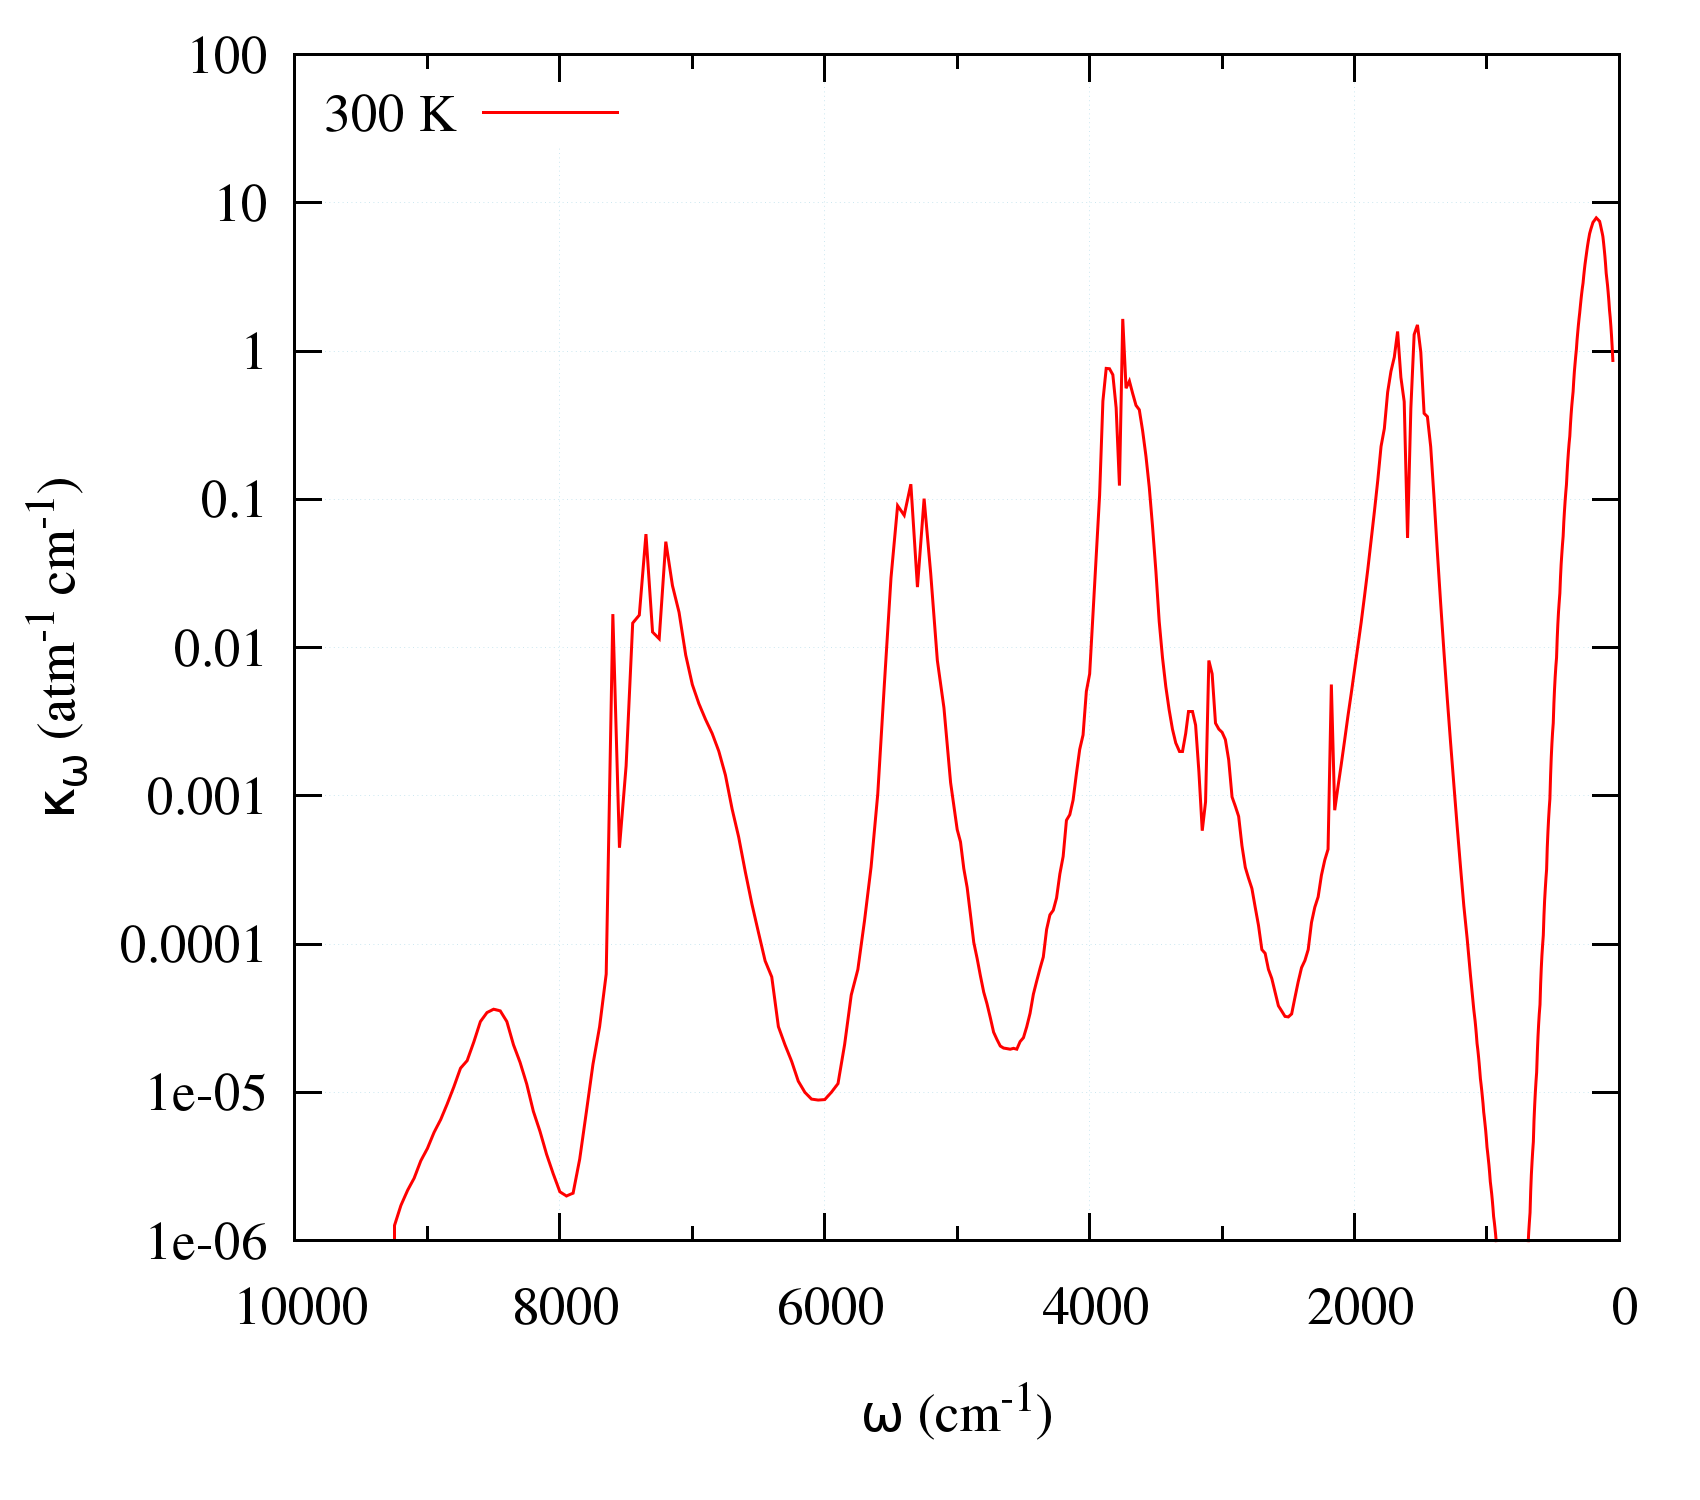
\includegraphics[height=2.5in]{Figures/H2O_300K.png} &
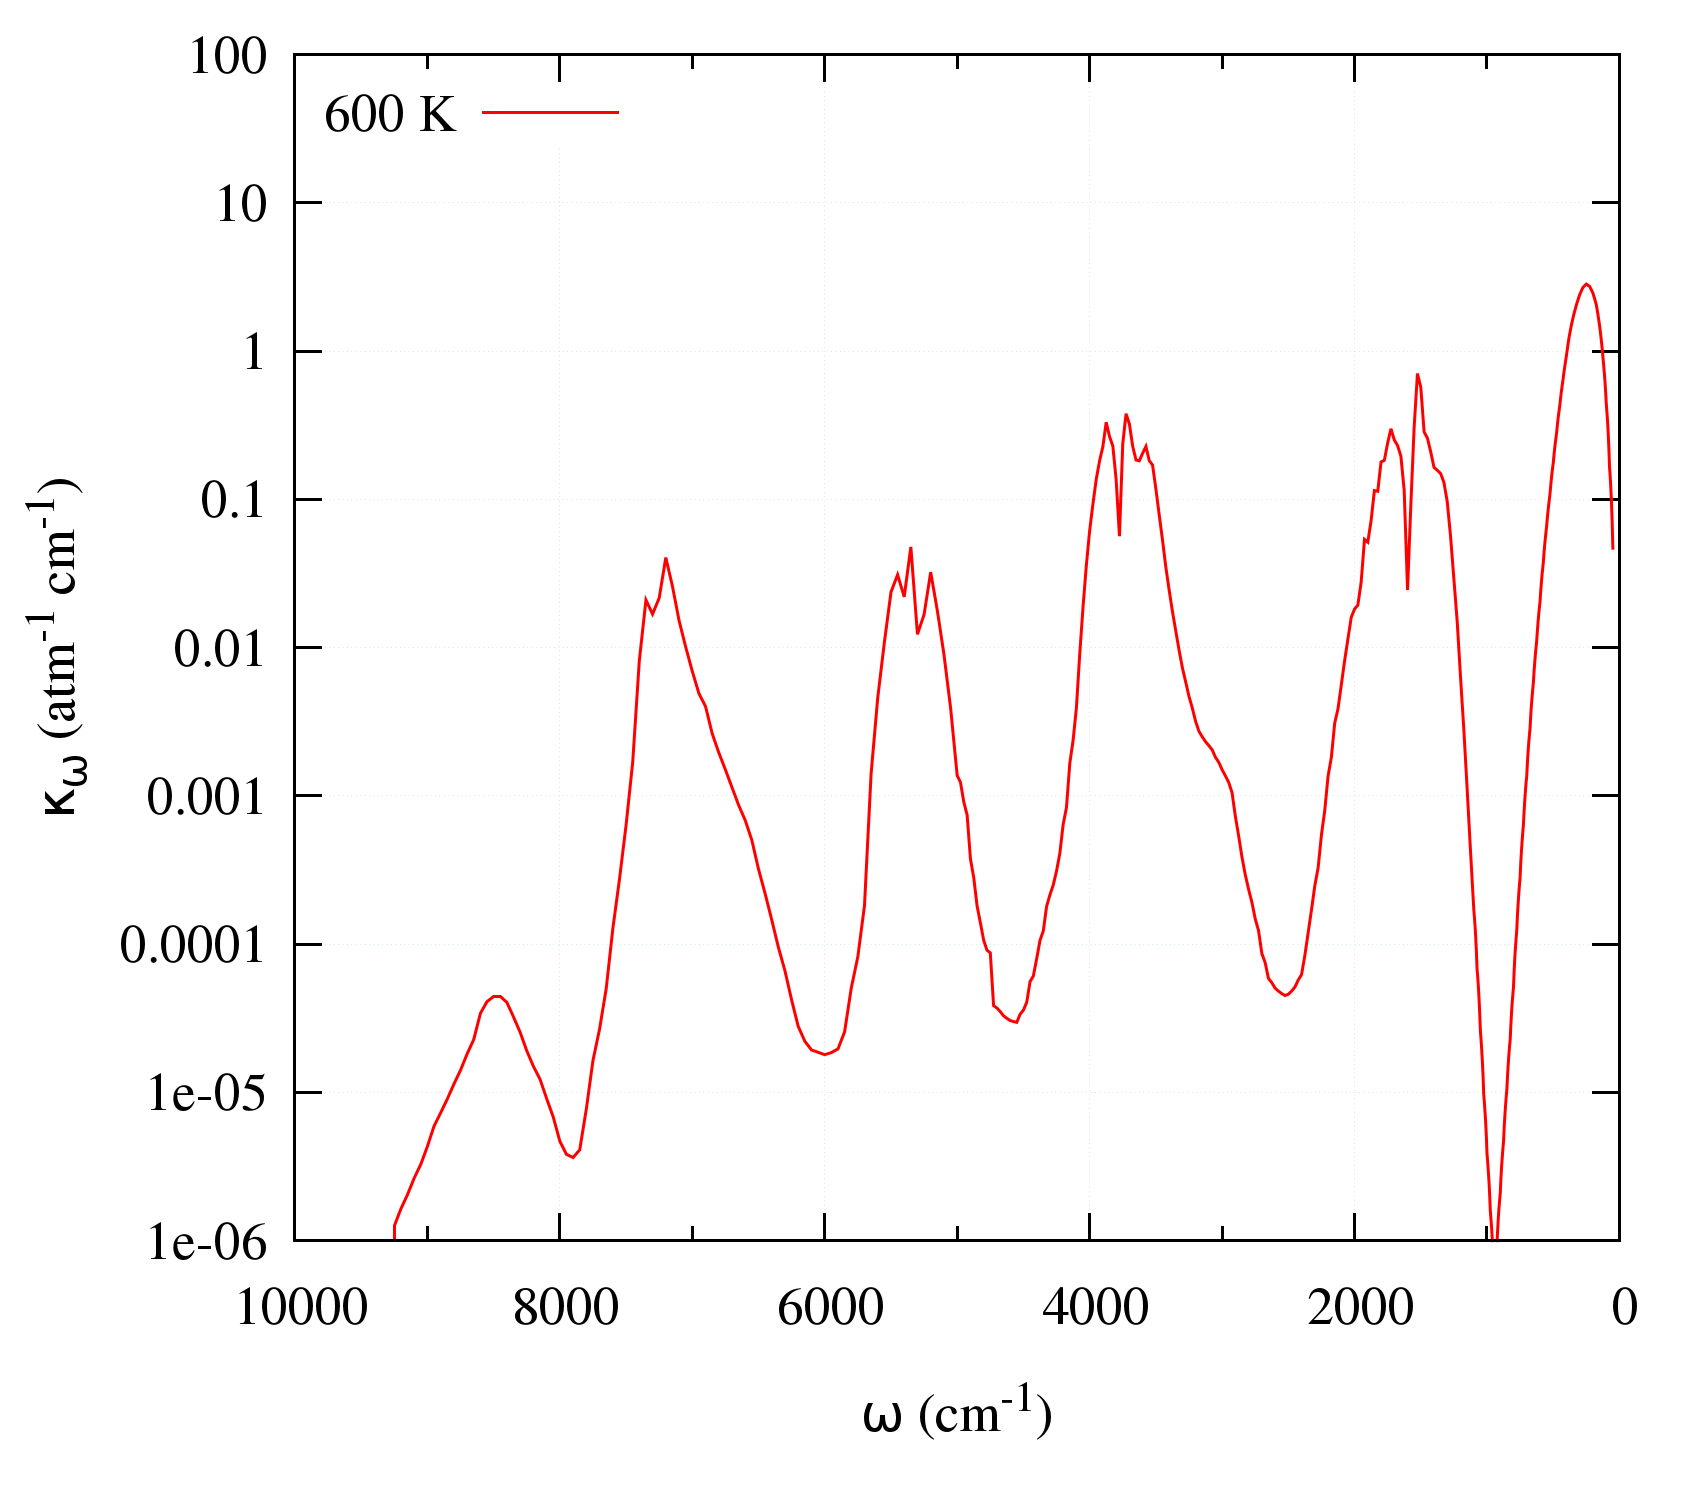
\includegraphics[height=2.5in]{Figures/H2O_600K.png} \\
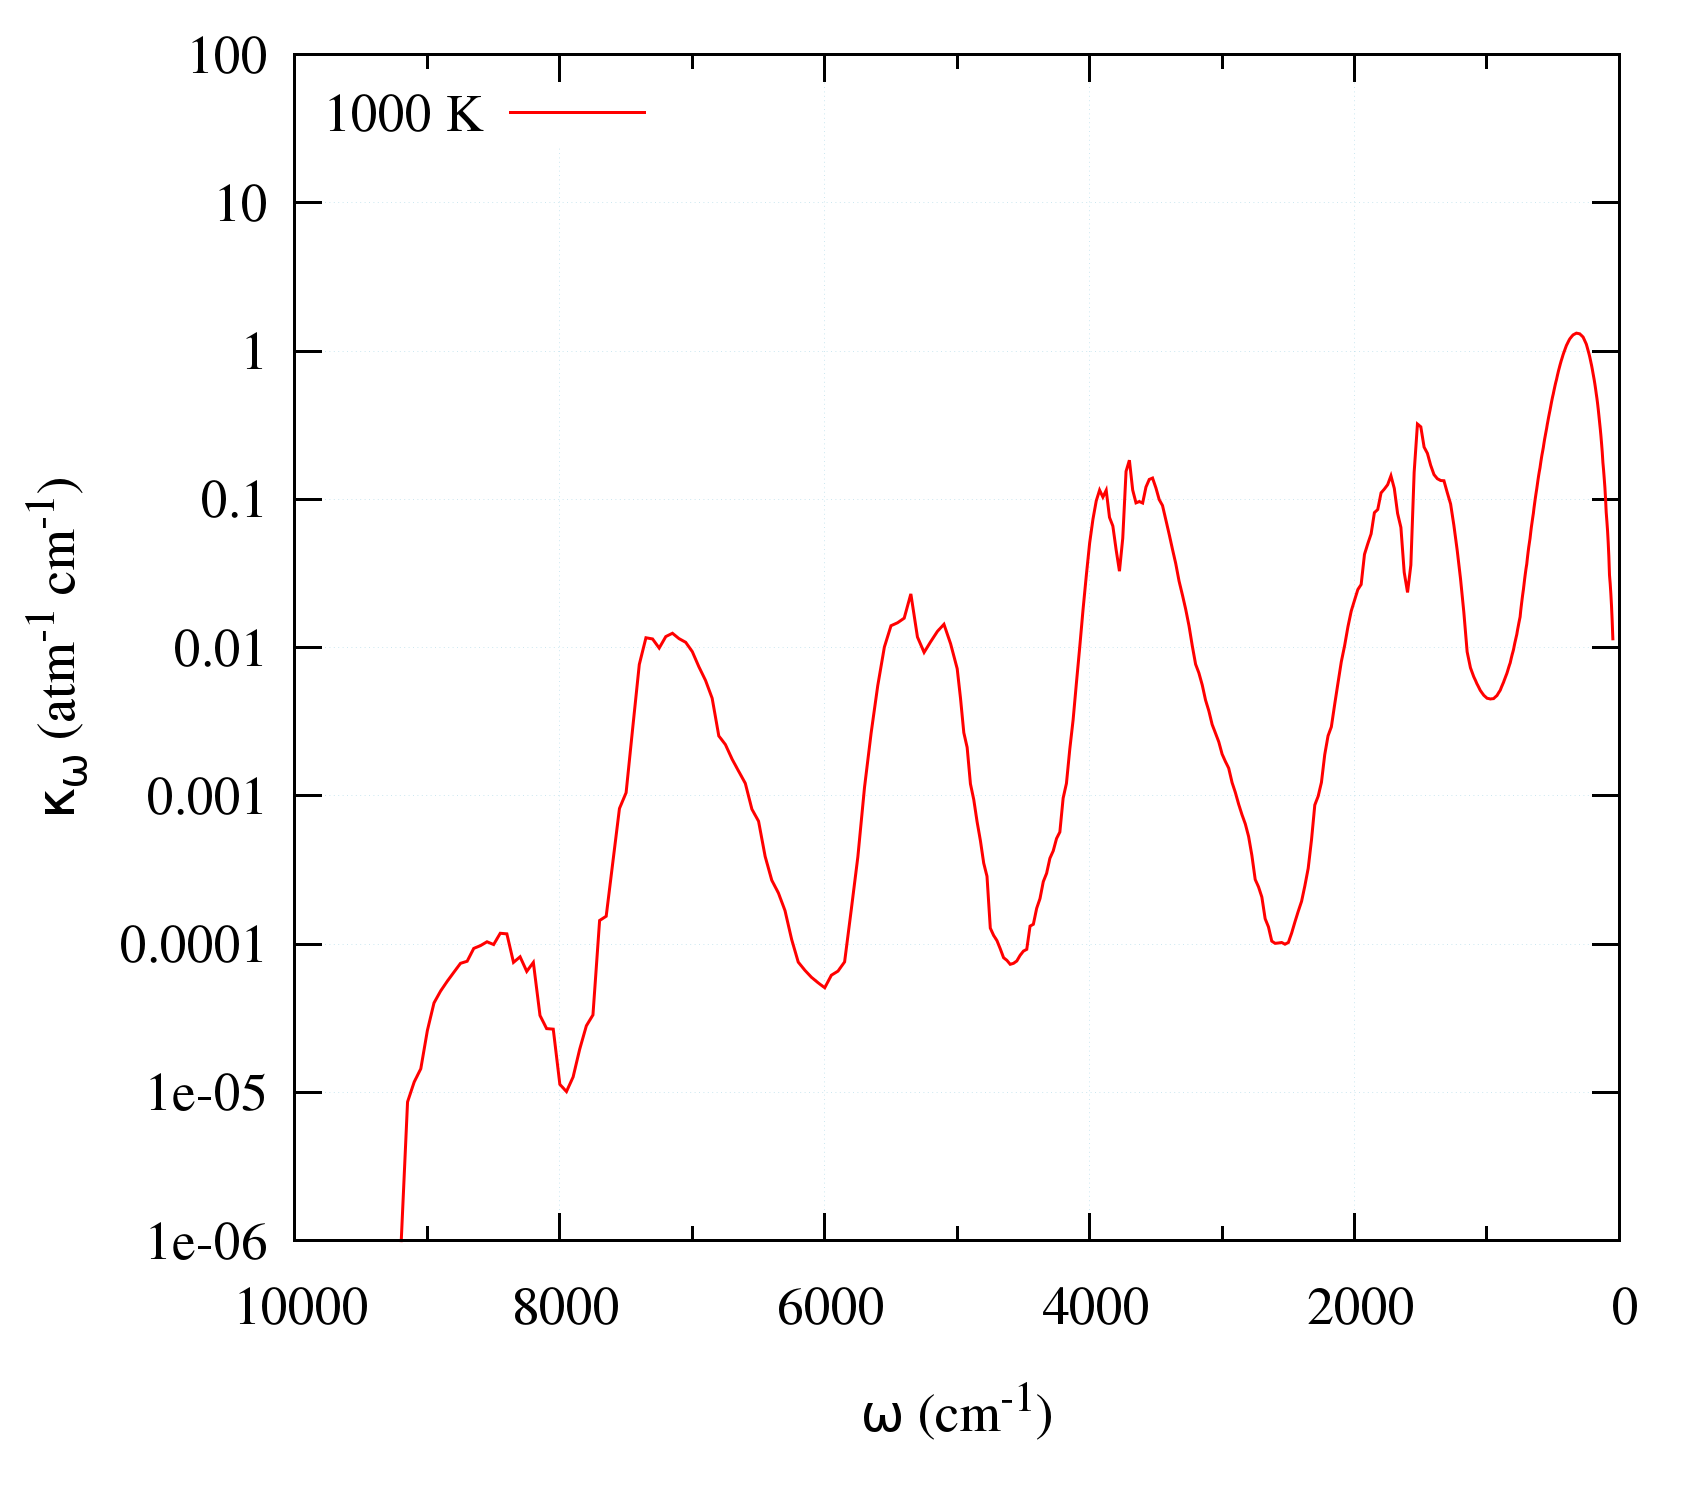
\includegraphics[height=2.5in]{Figures/H2O_1000K.png} &
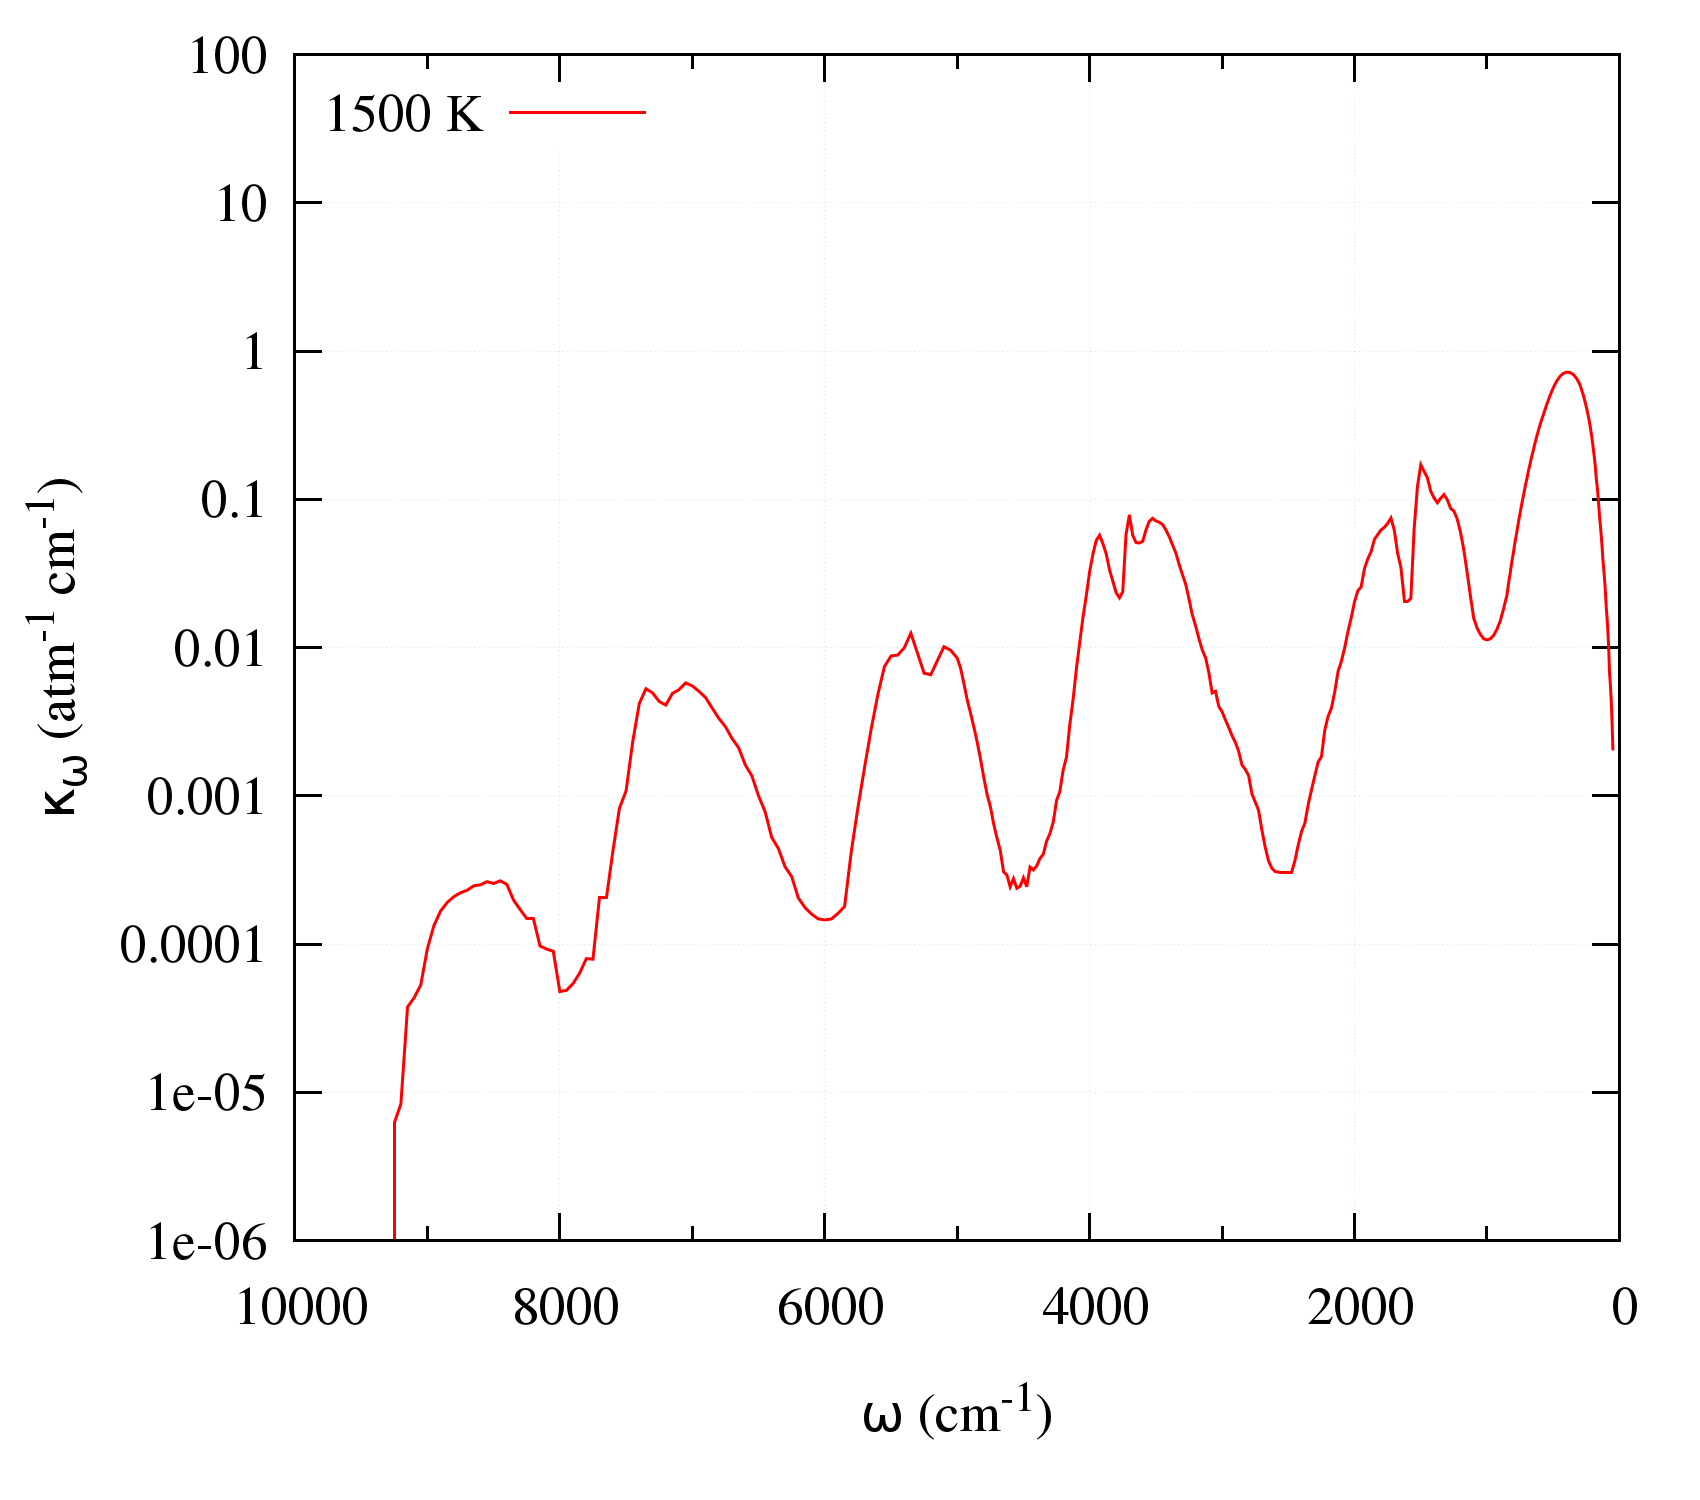
\includegraphics[height=2.5in]{Figures/H2O_1500K.png} \\
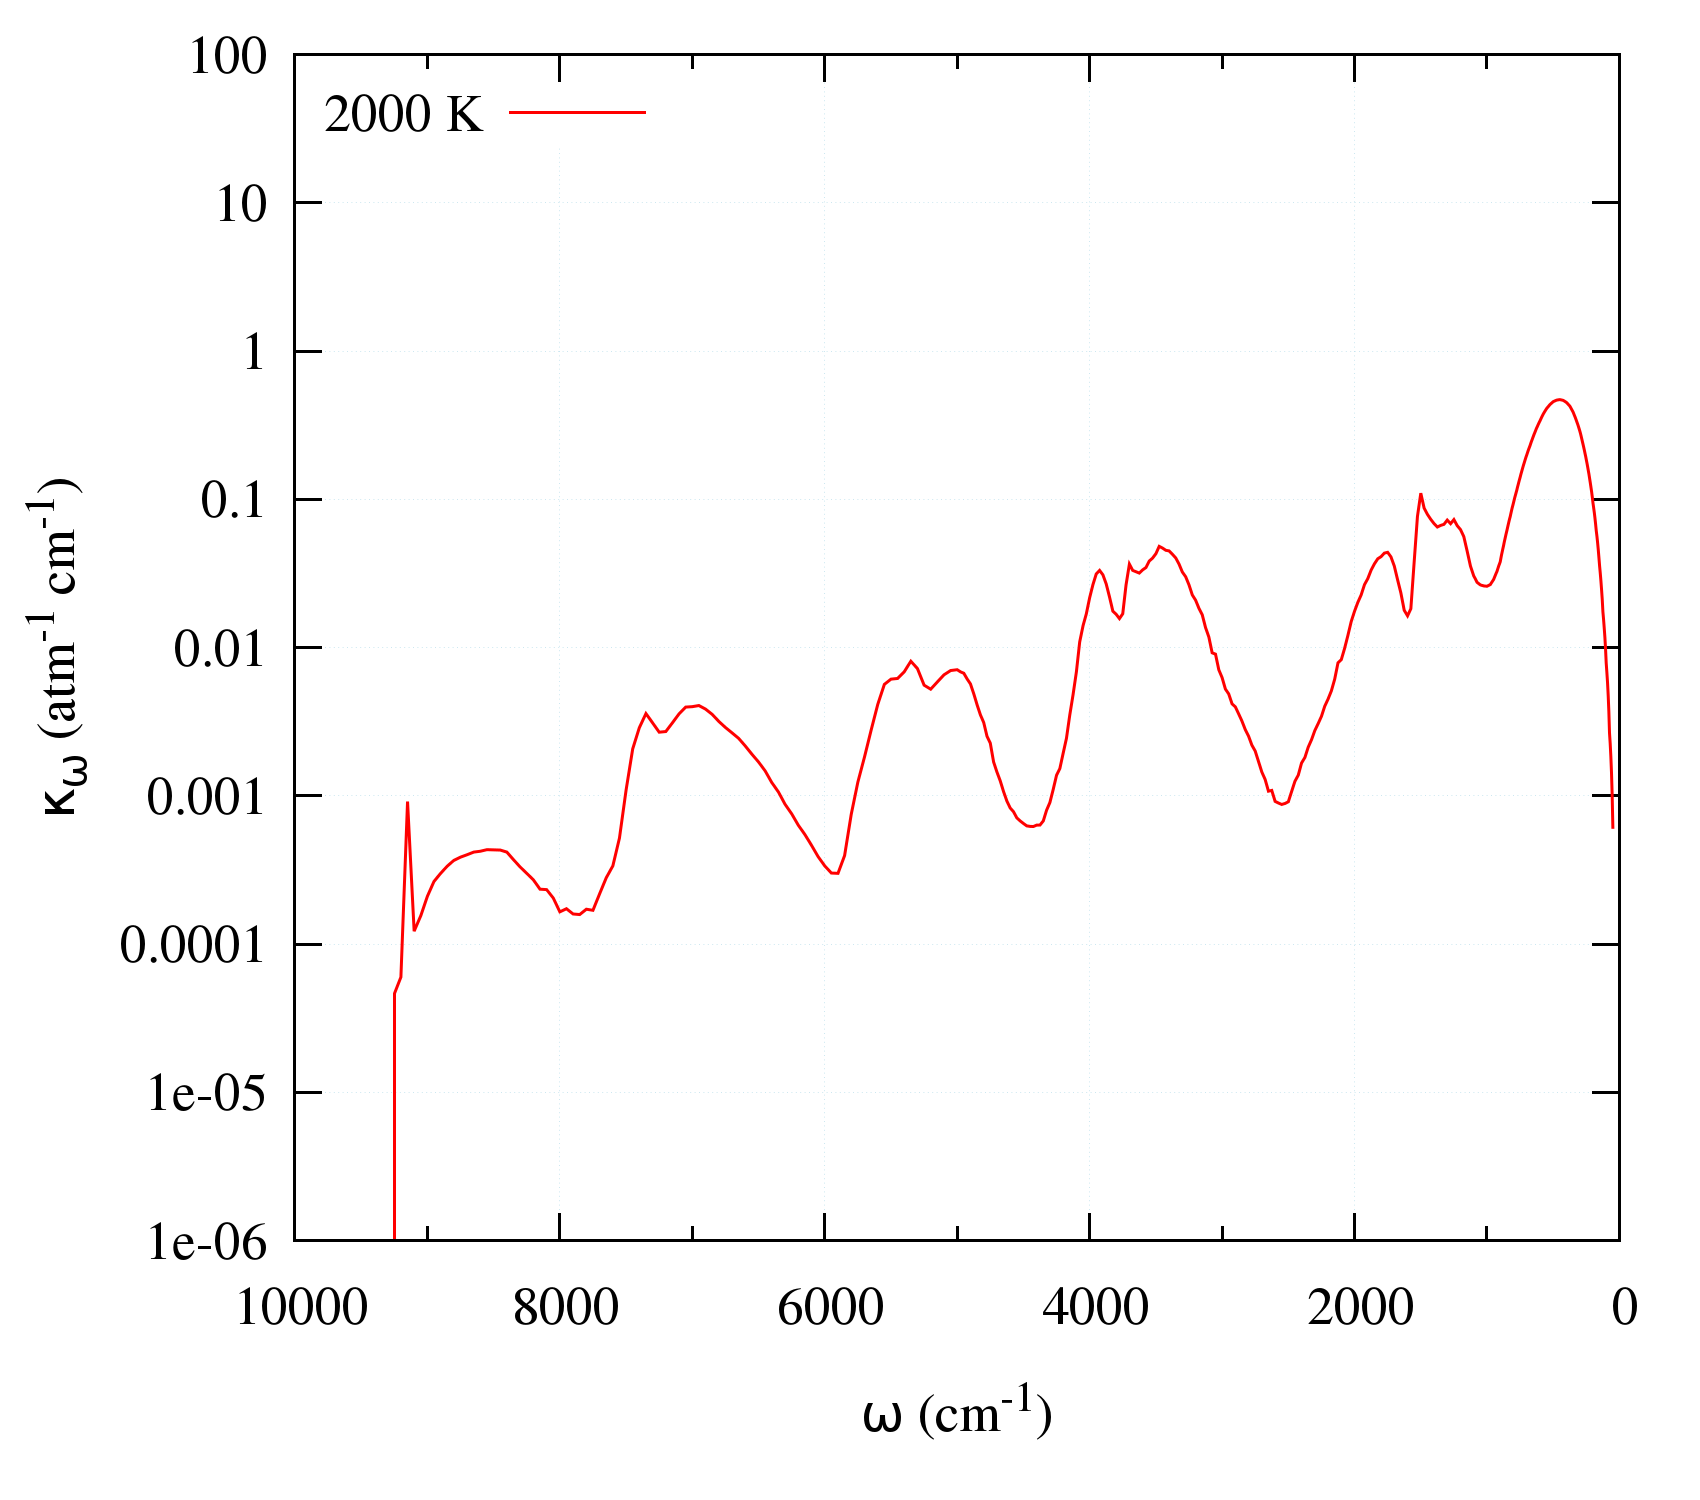
\includegraphics[height=2.5in]{Figures/H2O_2000K.png} &
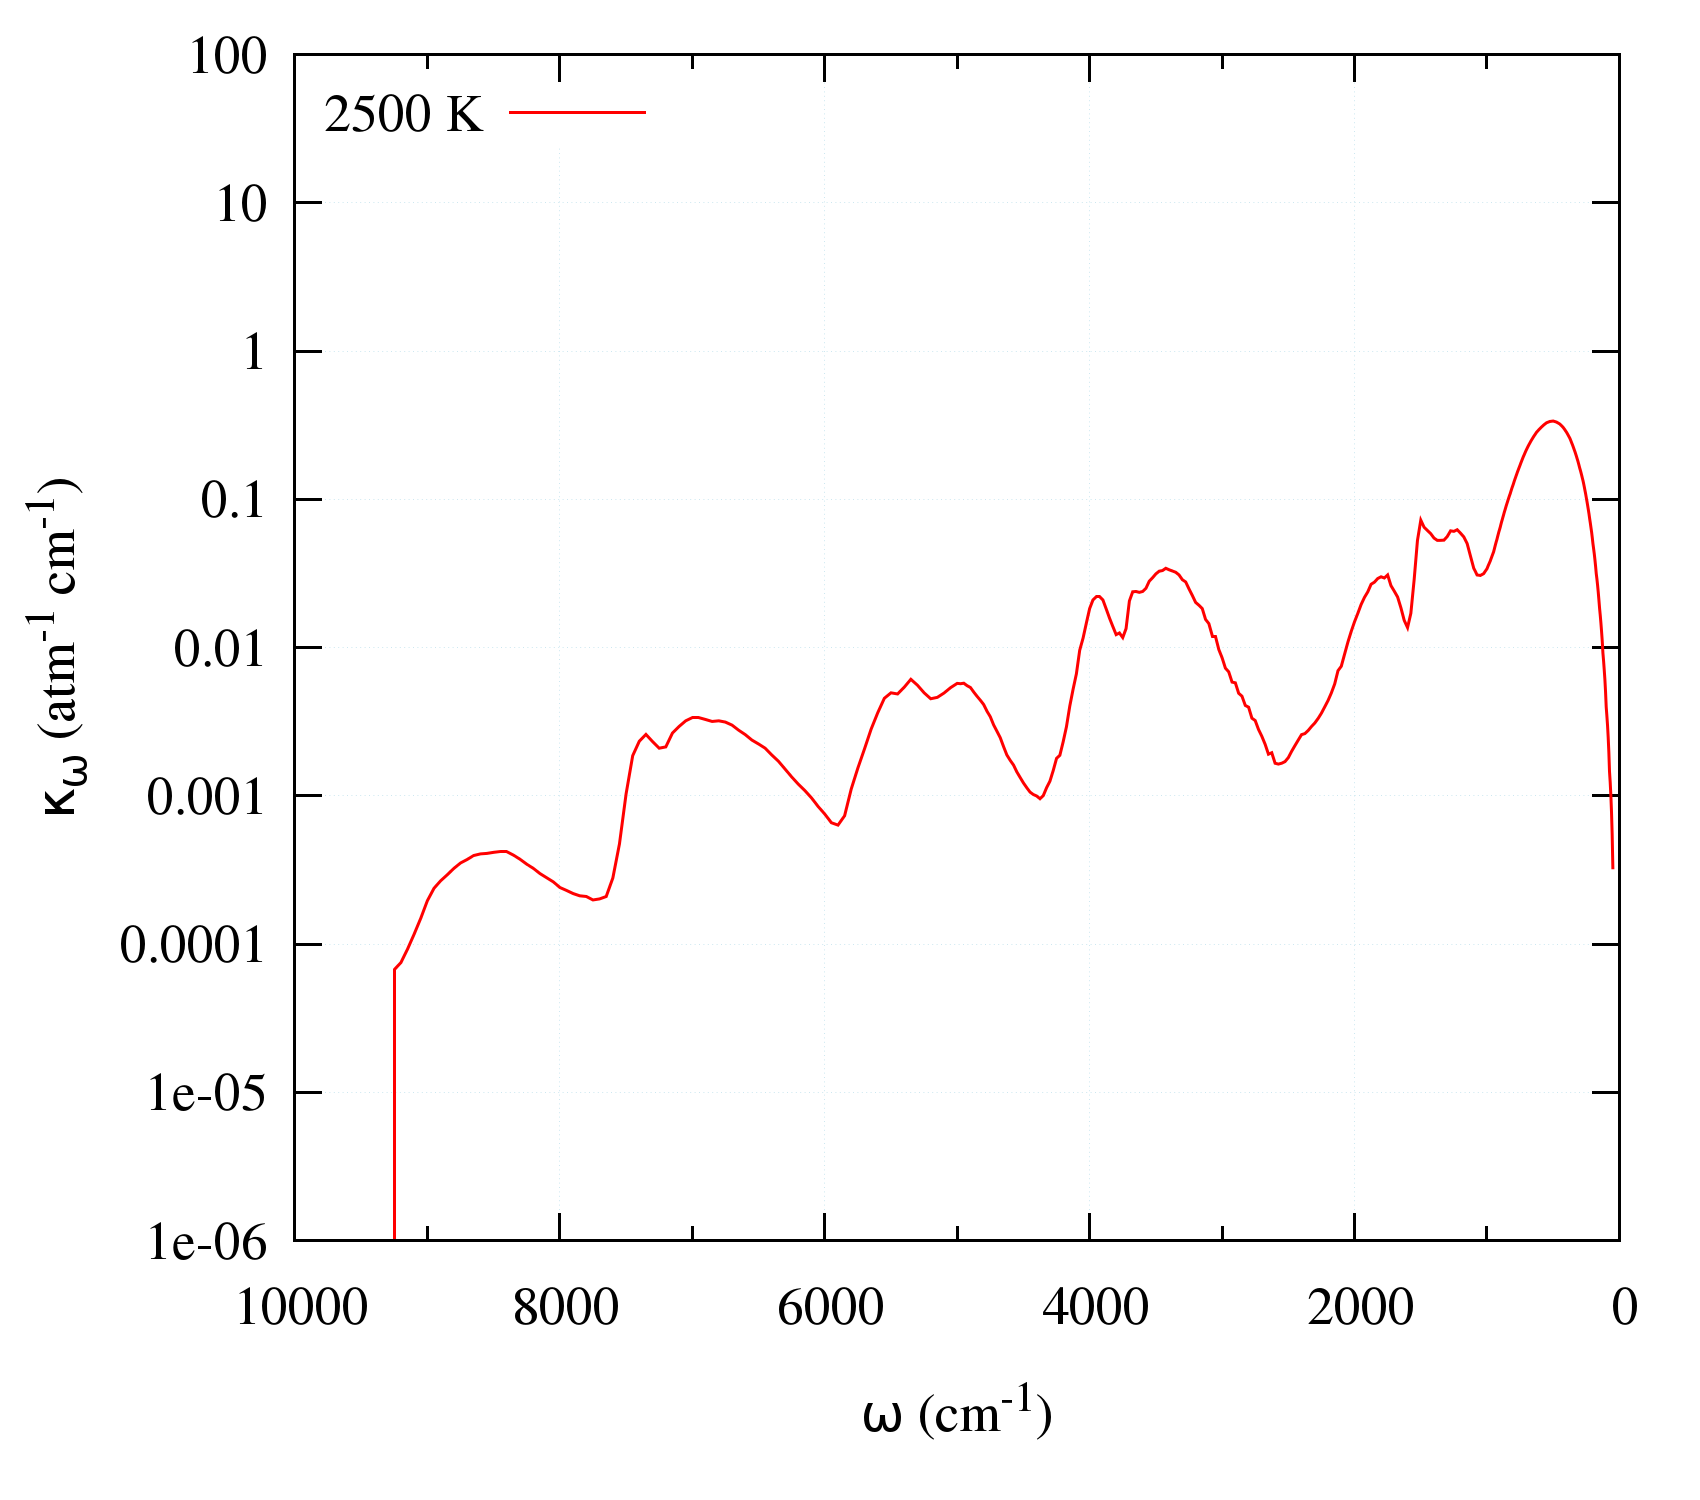
\includegraphics[height=2.5in]{Figures/H2O_2500K.png}
\end{tabular*}
\caption{Spectral variations of the $\rm H_2O$ mean absorption coefficient $\bar{\kappa}_{\om}$, in $\rm atm^{-1}.cm^{-1}$, at various temperatures as tabulated in RadCal.\label{fig:H2O_300-2500K}}
\end{figure}

To calculate the band overlap parameter $\beta$, the Lorentz HWHM is considered constant over the spectrum and is calculated using Eq.~\ref{eq:gamma_L}, while the effective line spacing is given by \cite{Ludwig1973}:
\begin{equation}
 d = \exp\left(0.7941 \sin\left(0.036 \omega- 8.043\right) + 2.294 + 0.3004 \times 10^{-2} T - 0.366 \times 10^{-6} T^2\right),
\end{equation}
where $T$ is the local temperature.


\clearpage

\section{Carbon dioxide: $\rm CO_2$}

Carbon dioxide is a linear, symmetric molecule. Its bond length is 115.98~pm in ground state, and its rotational constant is 0.3906~cm$^{-1}$. Because of the symmetry, $\rm CO_2$ has no permanent dipole moment. It has four vibrational modes, but only two fundamental IR vibration modes. Five distinct bands are included in RadCal (four are calculated, one is tabulated), see Table \ref{Table::CO2}. All the bands are modeled after the Goody model.

\begin{table}[h!]
    \centering
    \caption{Spectral bands of $\rm CO_2$ included in RadCal.}
    \label{Table::CO2}
    \begin{tabular}{|c|c|c|c|l|}
      \hline
      Band \# & \multicolumn{2}{|l|}{Bounds (cm$\rm ^{-1}$) } & Method & Notes: \\
      \cline{1-5}
      1 &  500 & 880  & tabulated&  15 $\mu$m region - strong (for atmospheric application)\\
      2 &  880 & 1100 & modeled  & 10 $\mu$m region\\
      3 & 1975 & 2475 & modeled  & 4.9 and 4.3 $\mu$m region - very strong\\
      4 & 3050 & 3800 & modeled  & 2.7 $\mu$m region - important for fire application\\
      5 & 4550 & 5275 & modeled  & 2.0 $\mu$m region\\
      \hline
    \end{tabular}
\end{table}

\begin{figure}[p]
\begin{tabular*}{\textwidth}{l@{\extracolsep{\fill}}r}
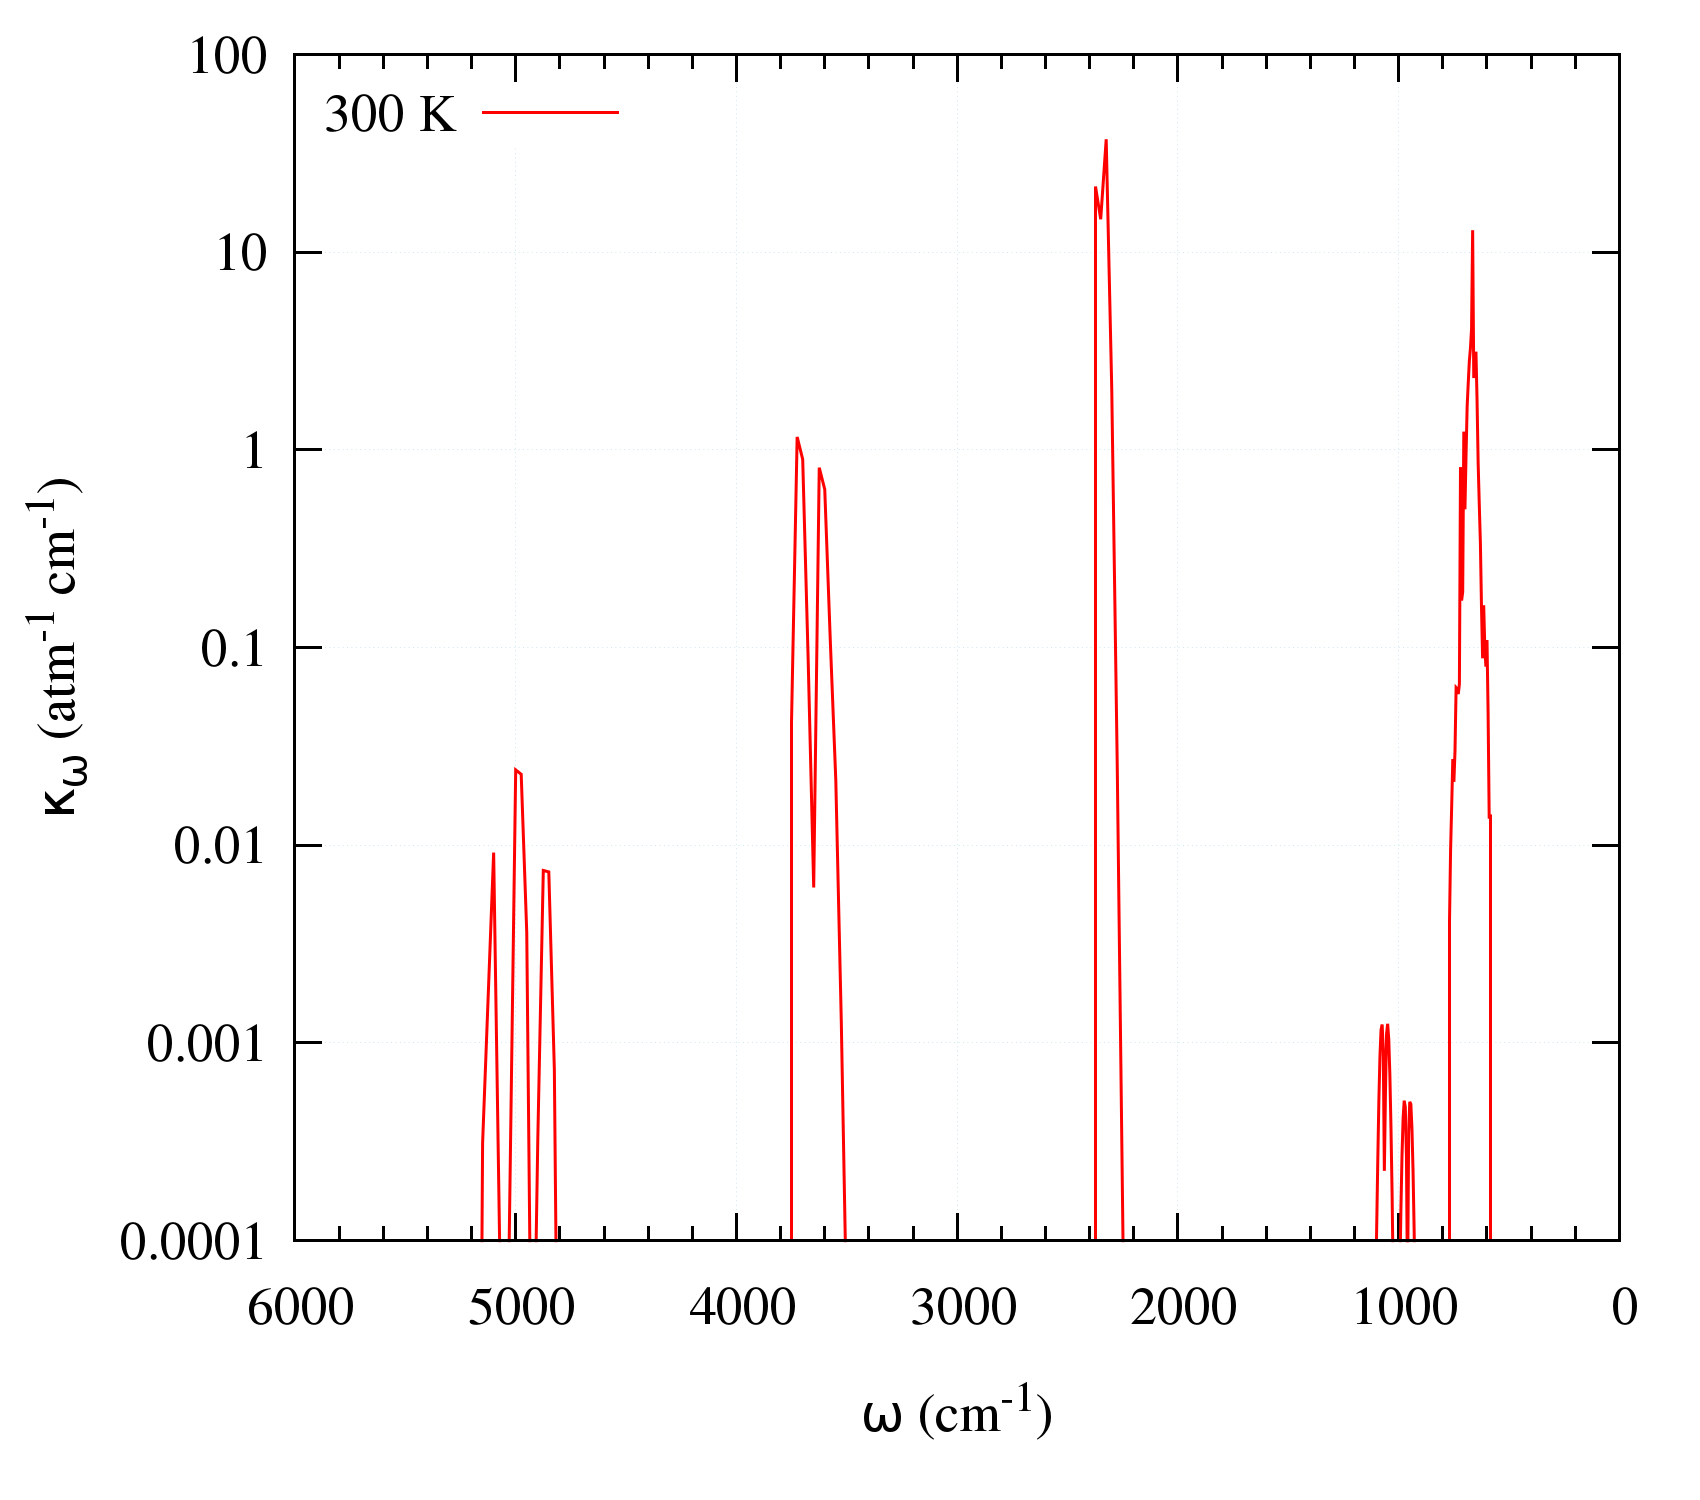
\includegraphics[height=2.5in]{Figures/CO2_300K.png} &
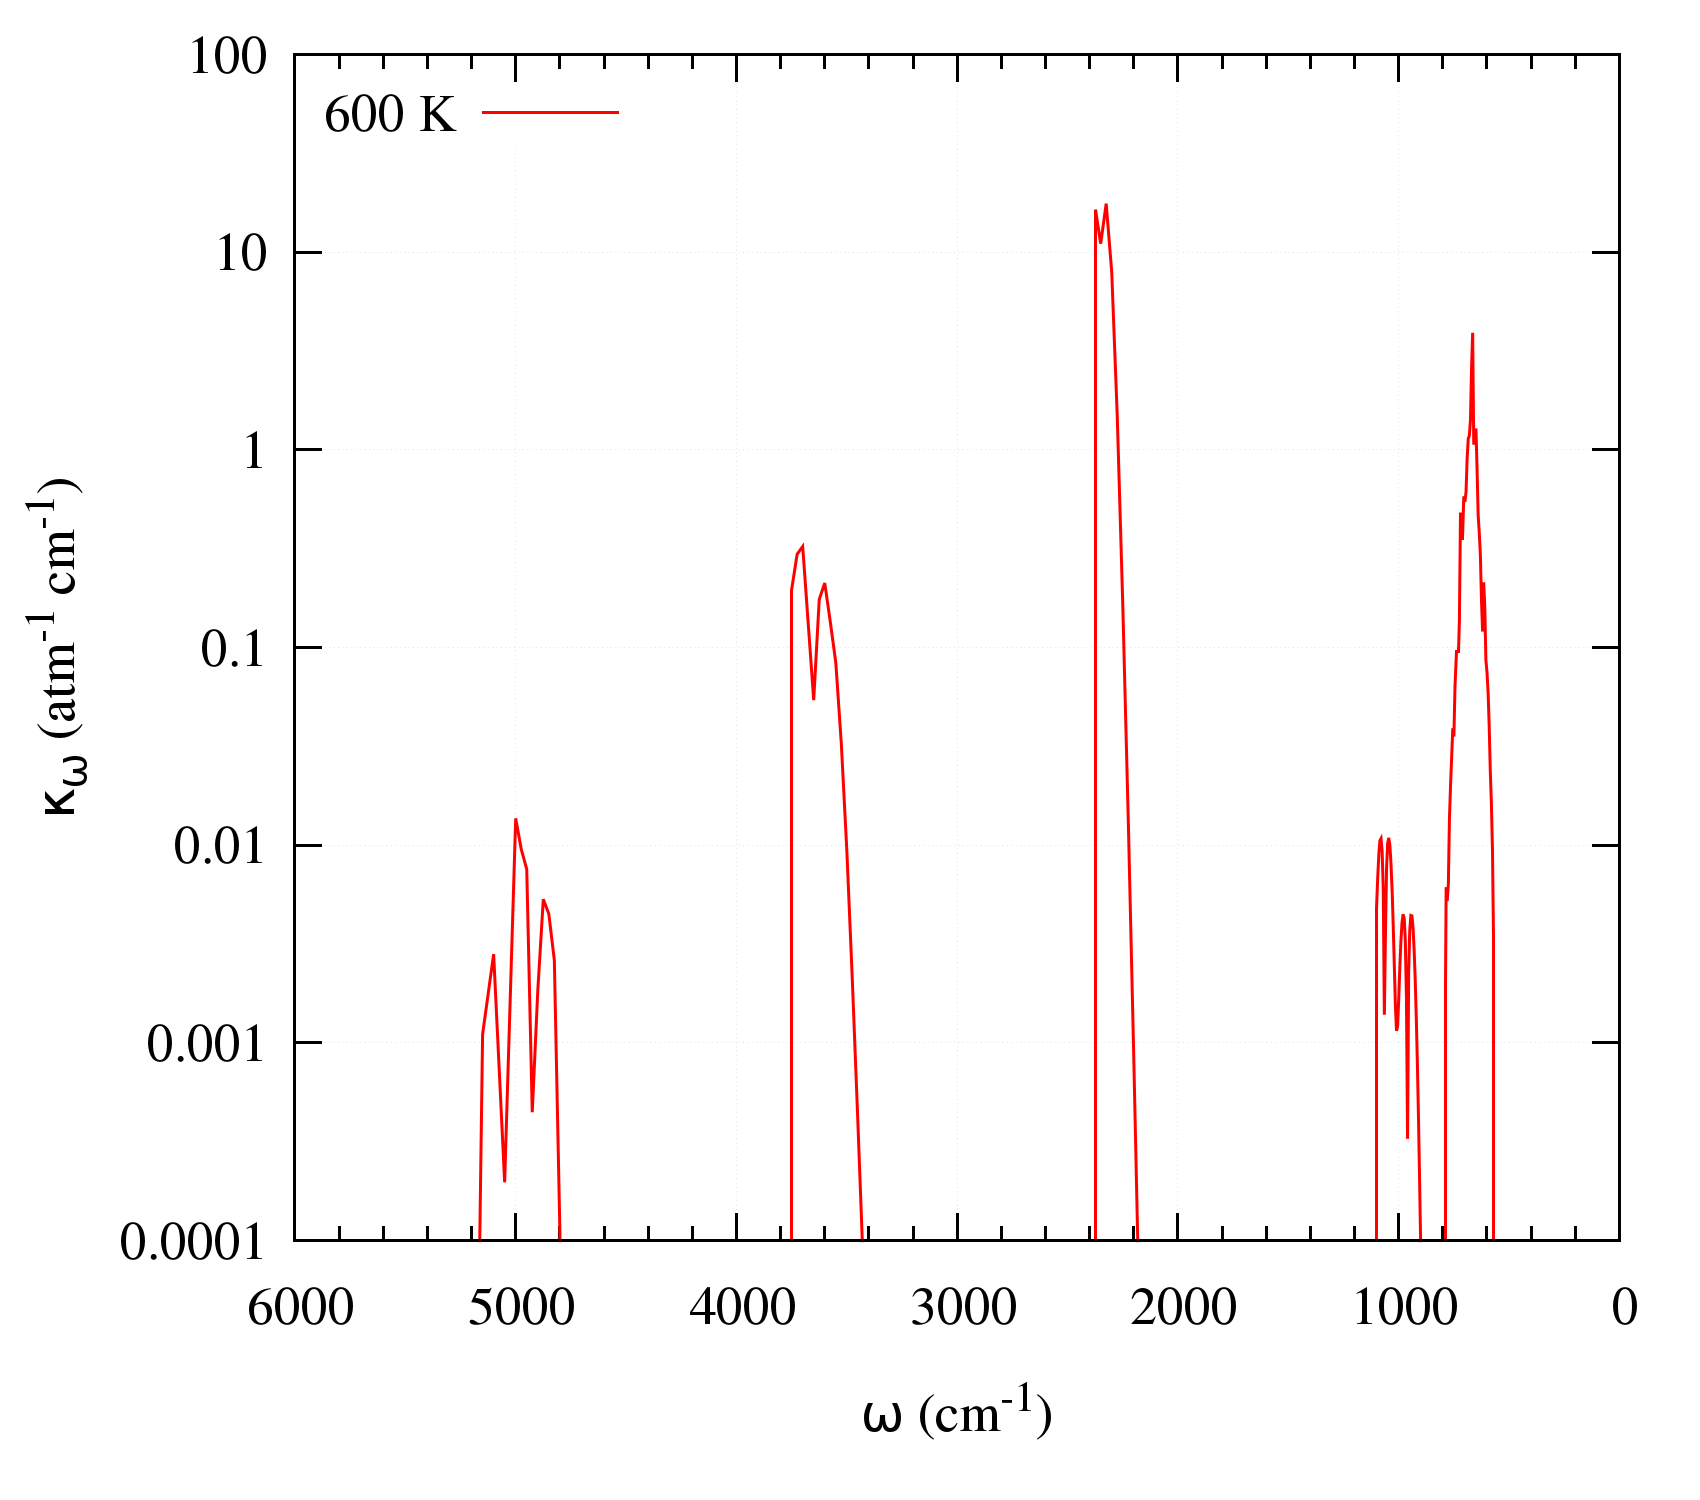
\includegraphics[height=2.5in]{Figures/CO2_600K.png} \\
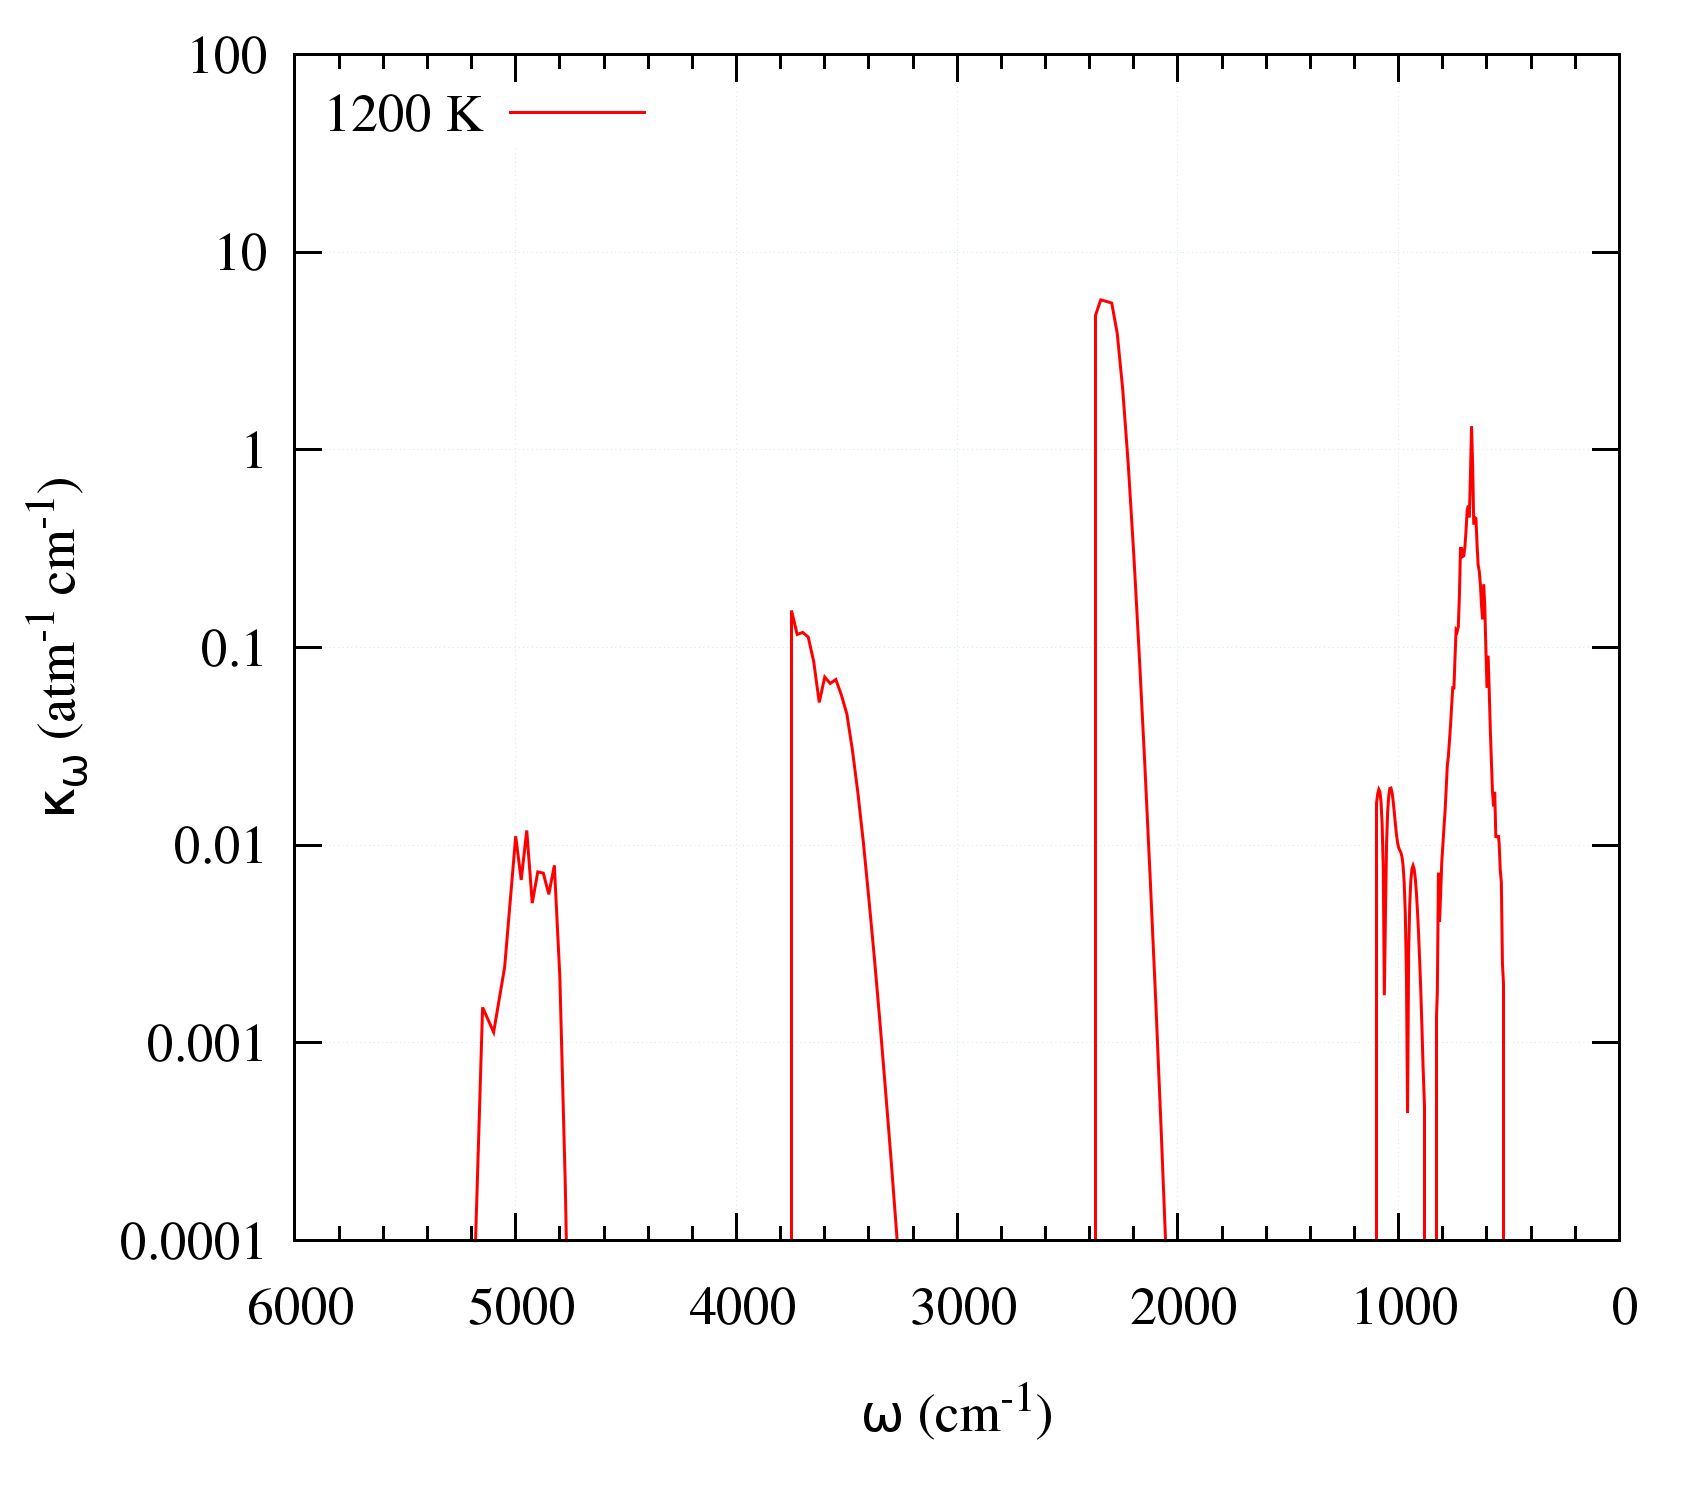
\includegraphics[height=2.5in]{Figures/CO2_1200K.png} &
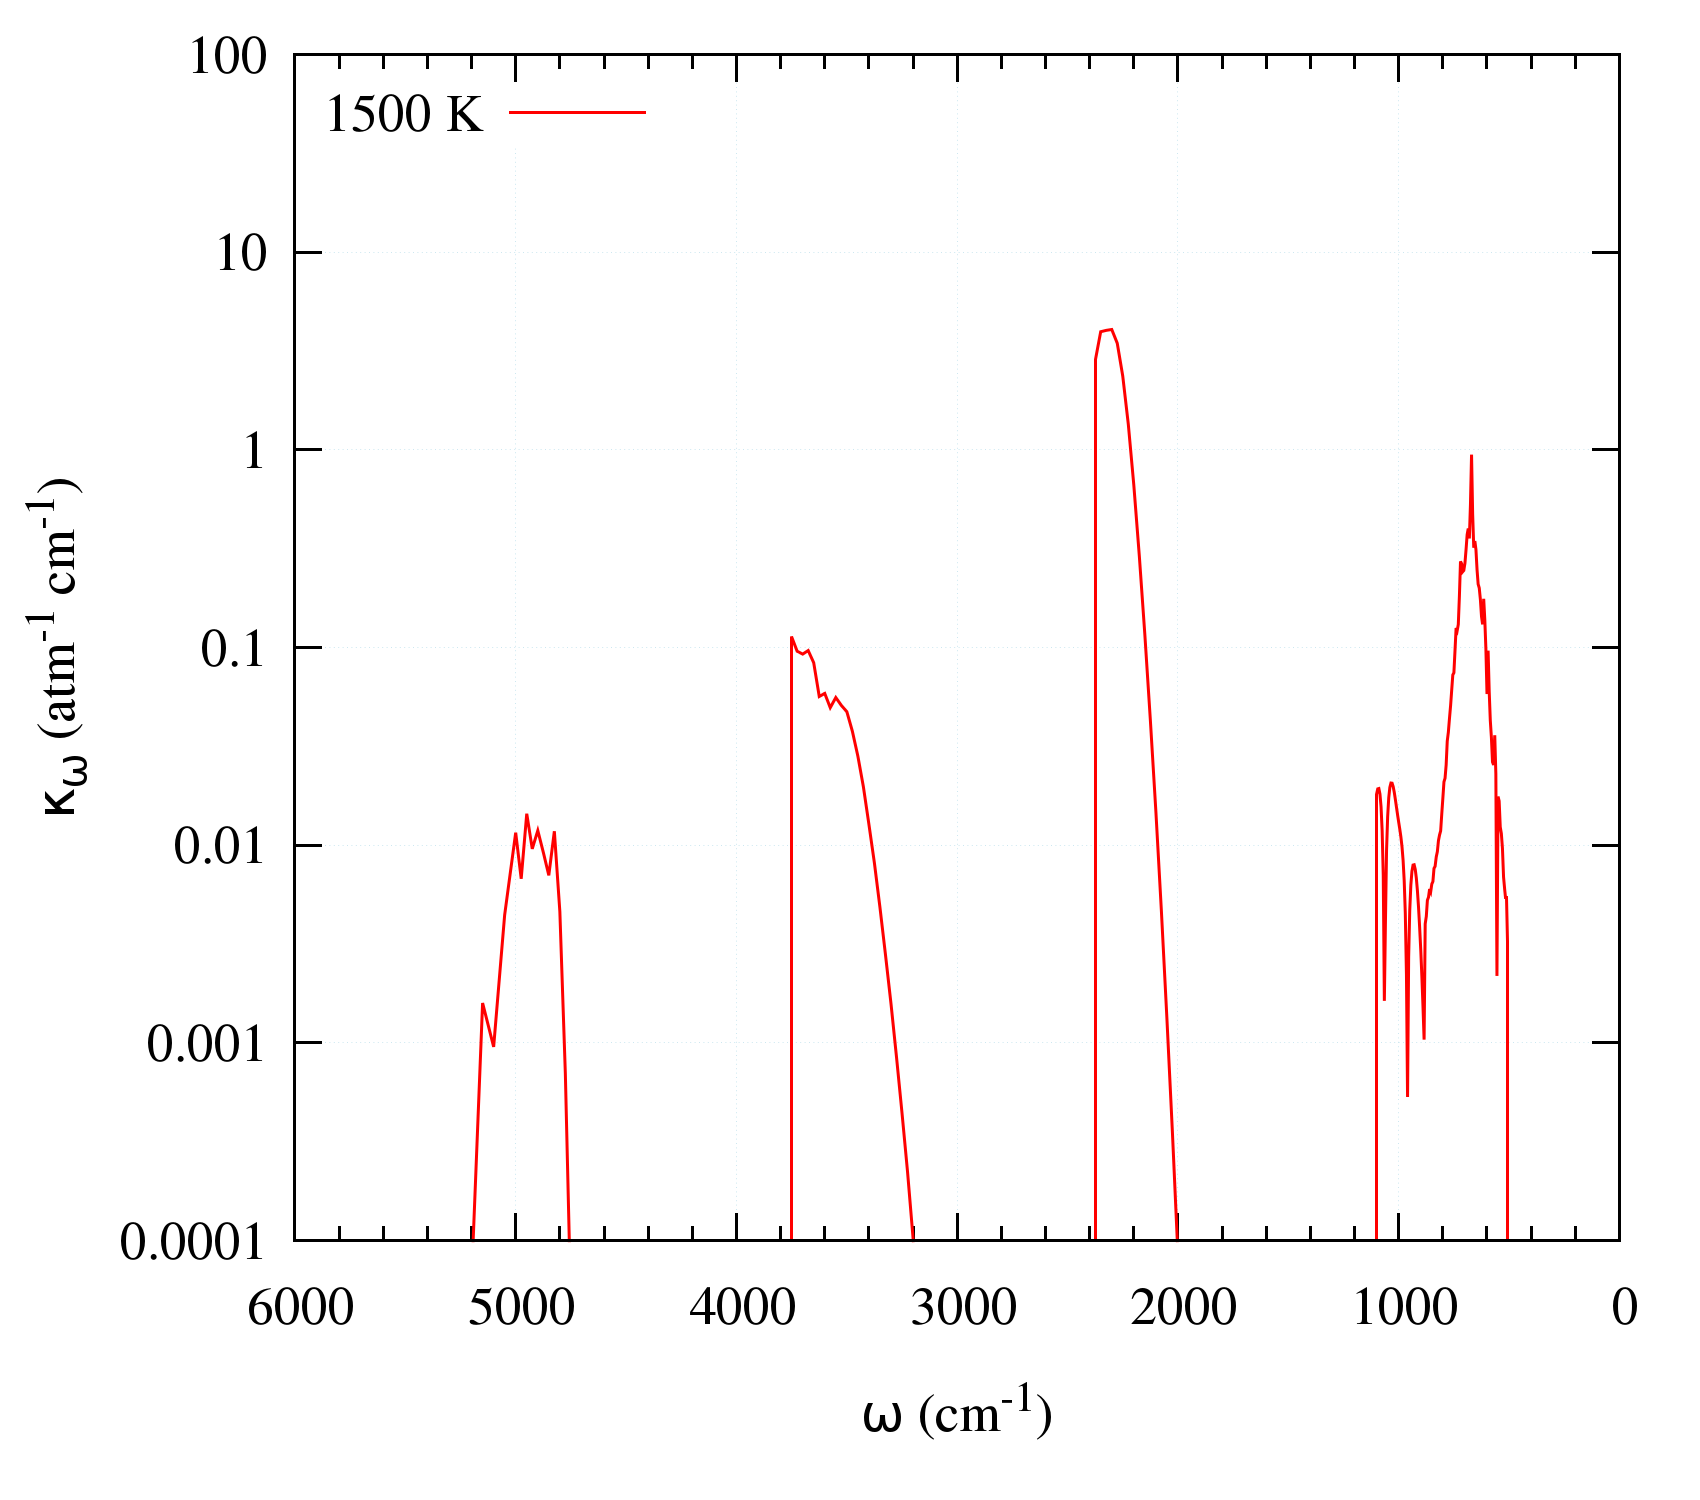
\includegraphics[height=2.5in]{Figures/CO2_1500K.png} \\
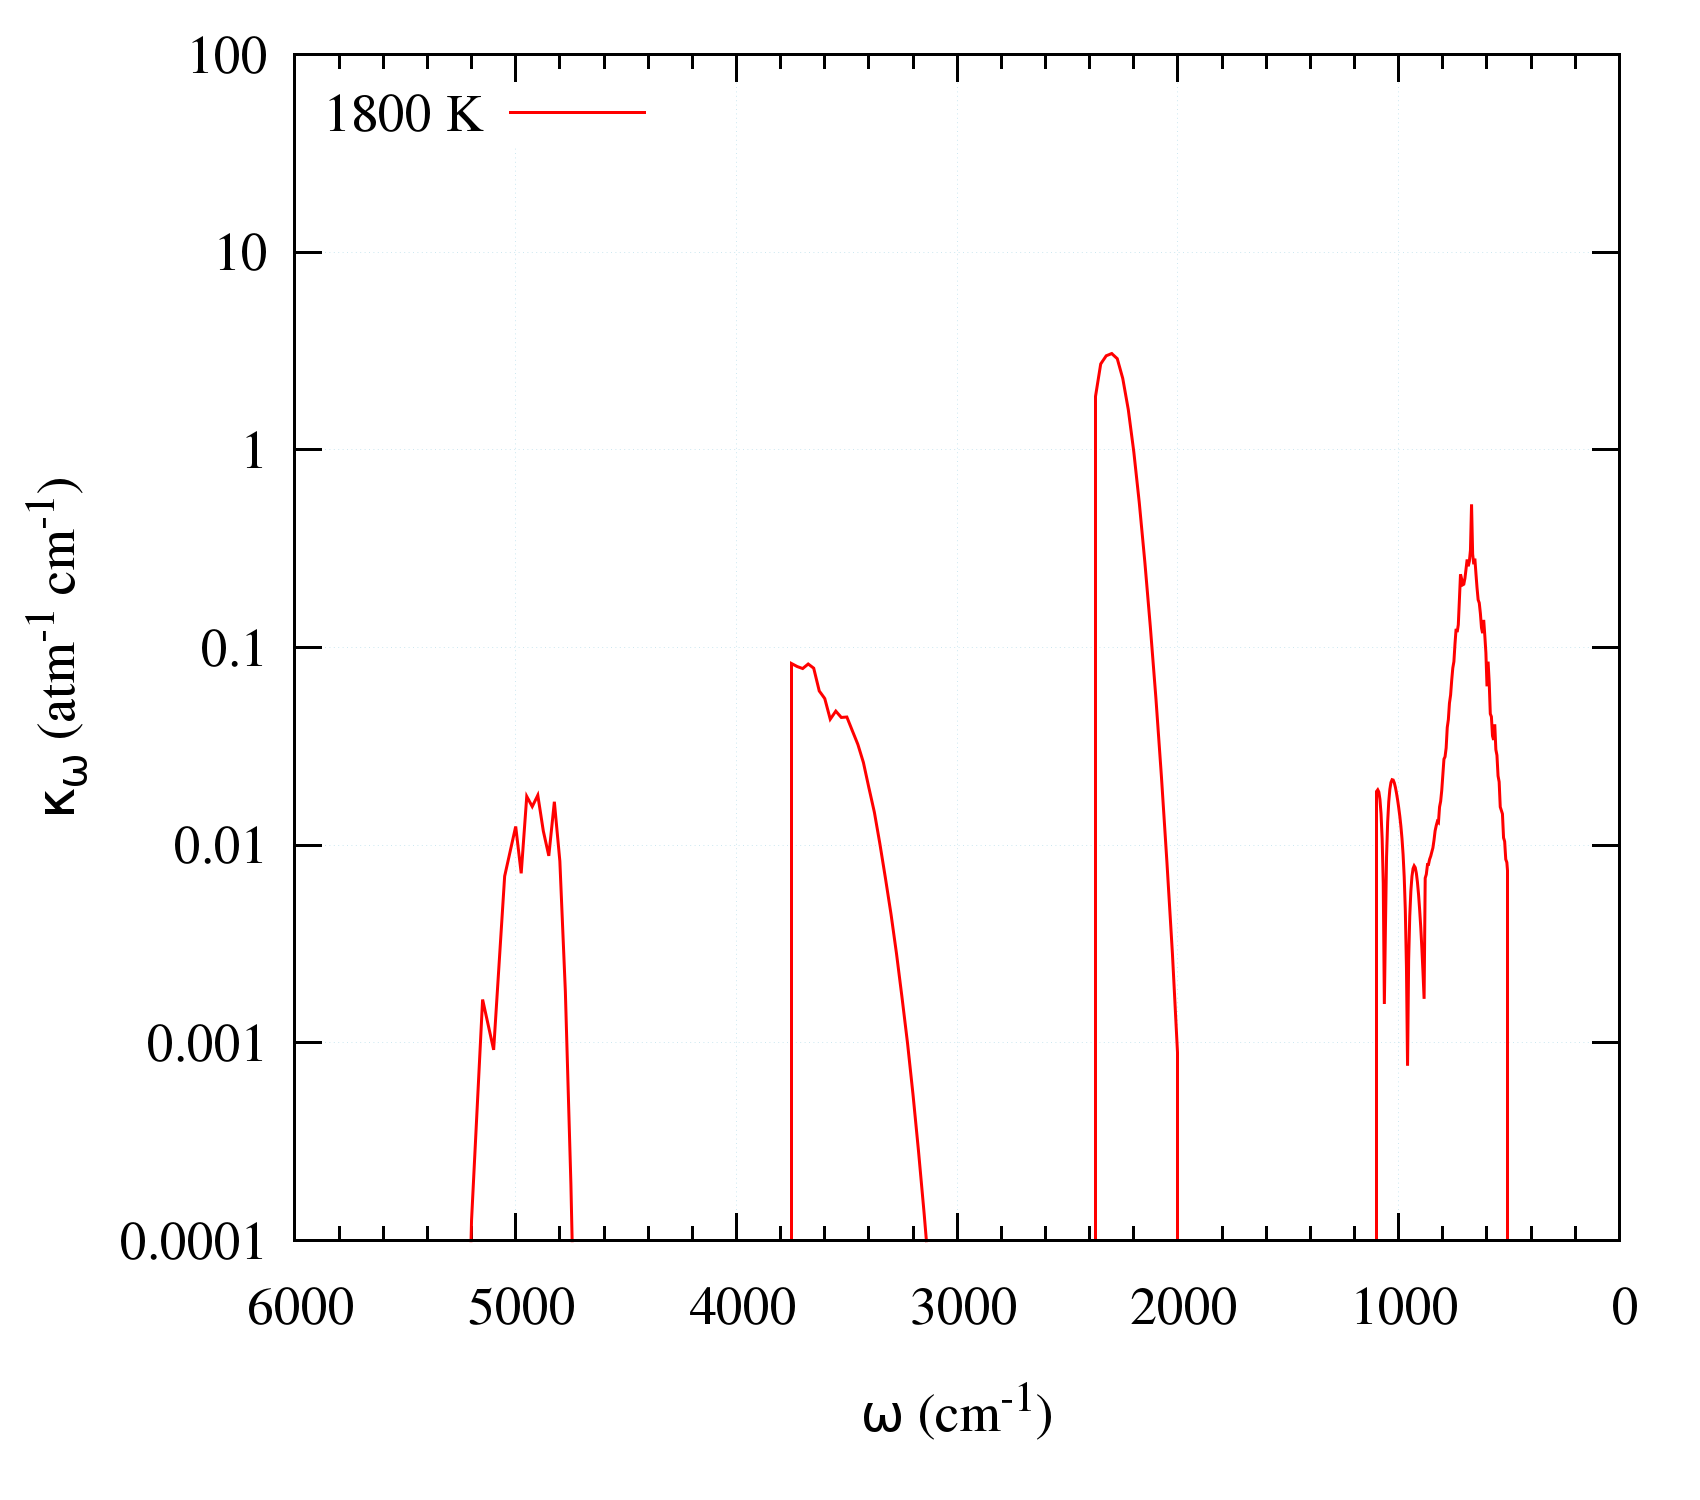
\includegraphics[height=2.5in]{Figures/CO2_1800K.png} &
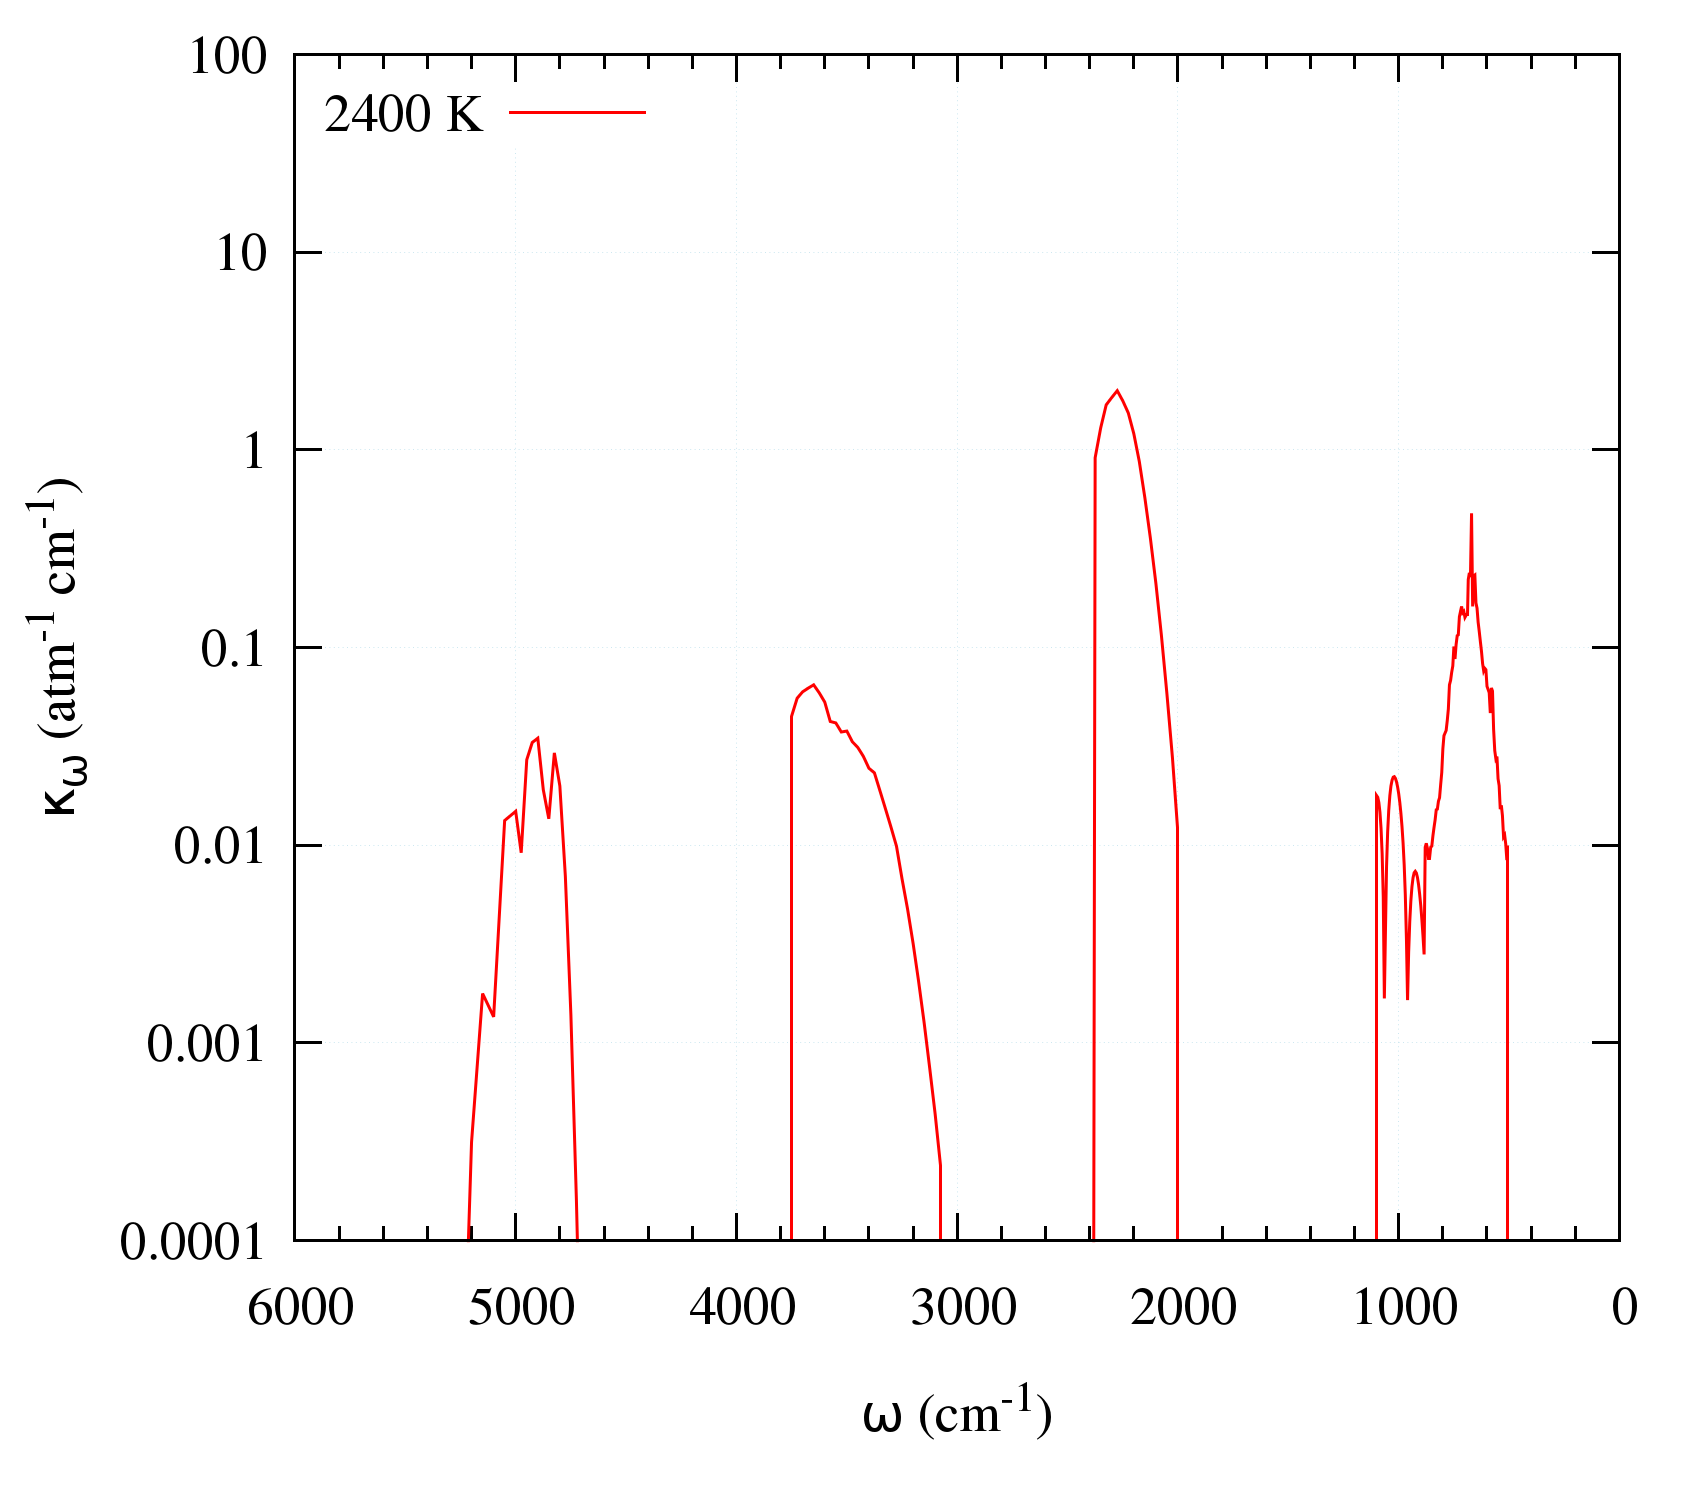
\includegraphics[height=2.5in]{Figures/CO2_2400K.png}
\end{tabular*}
\caption{Spectral variations of the $\rm CO_2$ mean absorption coefficient $\bar{\kappa}_{\om}$, in $\rm atm^{-1}.cm^{-1}$, at various temperatures as tabulated in RadCal.\label{fig:CO2_300-2500K}}
\end{figure}

The strongest band in the $\rm CO_2$ spectrum is Band~3. At 300~K, it has an integrated band intensity (see Section~\ref{sec:integrated_intensity} for a definition of this quantity) of 2963~atm$^{-1}$cm$^{-2}$. The tabulated data (mean absorption coefficient $\bar{\kappa}_{\om}$) were obtained from experiments for the following temperatures: 300, 600, 1200, 1500, 1800, 2400~K. The modeled bands use the harmonic oscillator approximation. All the bands uses the Goody statistical narrow band model. Figure~\ref{fig:CO2_300-2500K} to displays the mean absorption coefficient at 300, 600, 1200, 1500, 1800, 2400~K, as tabulated (Band 1) and modeled in RadCal (Bands 2 to 5).


\clearpage

\section{Carbon monoxide: $\rm CO$}

Carbon Monoxide is a diatomic molecule and as such, it has only one fundamental vibrational mode. RadCal includes one distinct band, the 1600--2400 band. It corresponds to the stretching of the triple bond $\rm C \equiv O$. This band is modeled and it uses the model from Malkmus and Thompson \cite{Malkmus1962}. It is based on the anharmonic oscillator model and uses band integrated intensity measurements. Figure~\ref{fig:CO_300-2500K} displays the spectral mean absorption coefficient of CO at 300~K and 2500~K.

\begin{figure}[ht]
\begin{tabular*}{\textwidth}{l@{\extracolsep{\fill}}r}
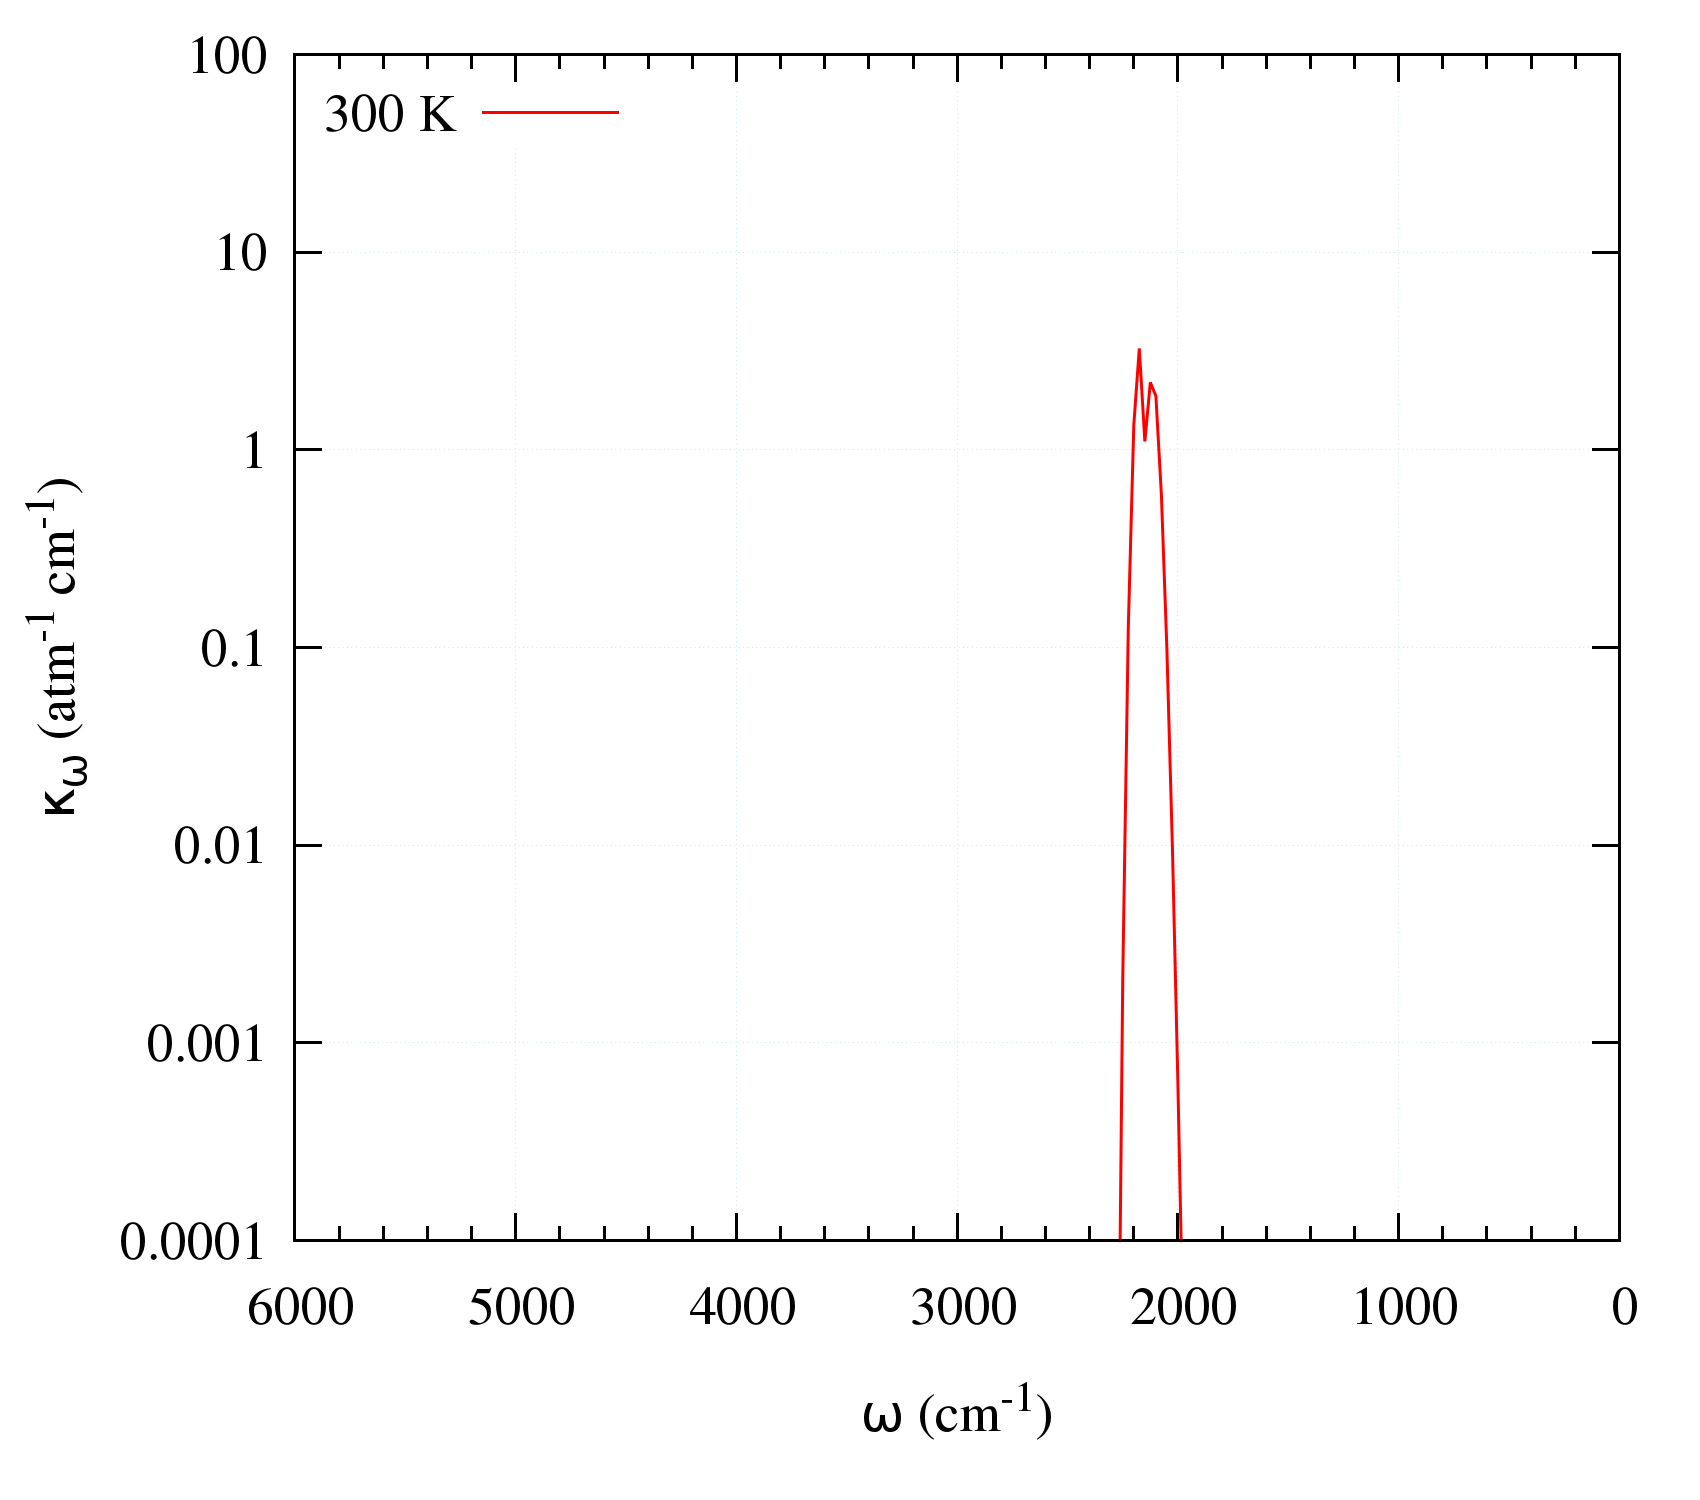
\includegraphics[height=2.5in]{Figures/CO_300K.png} &
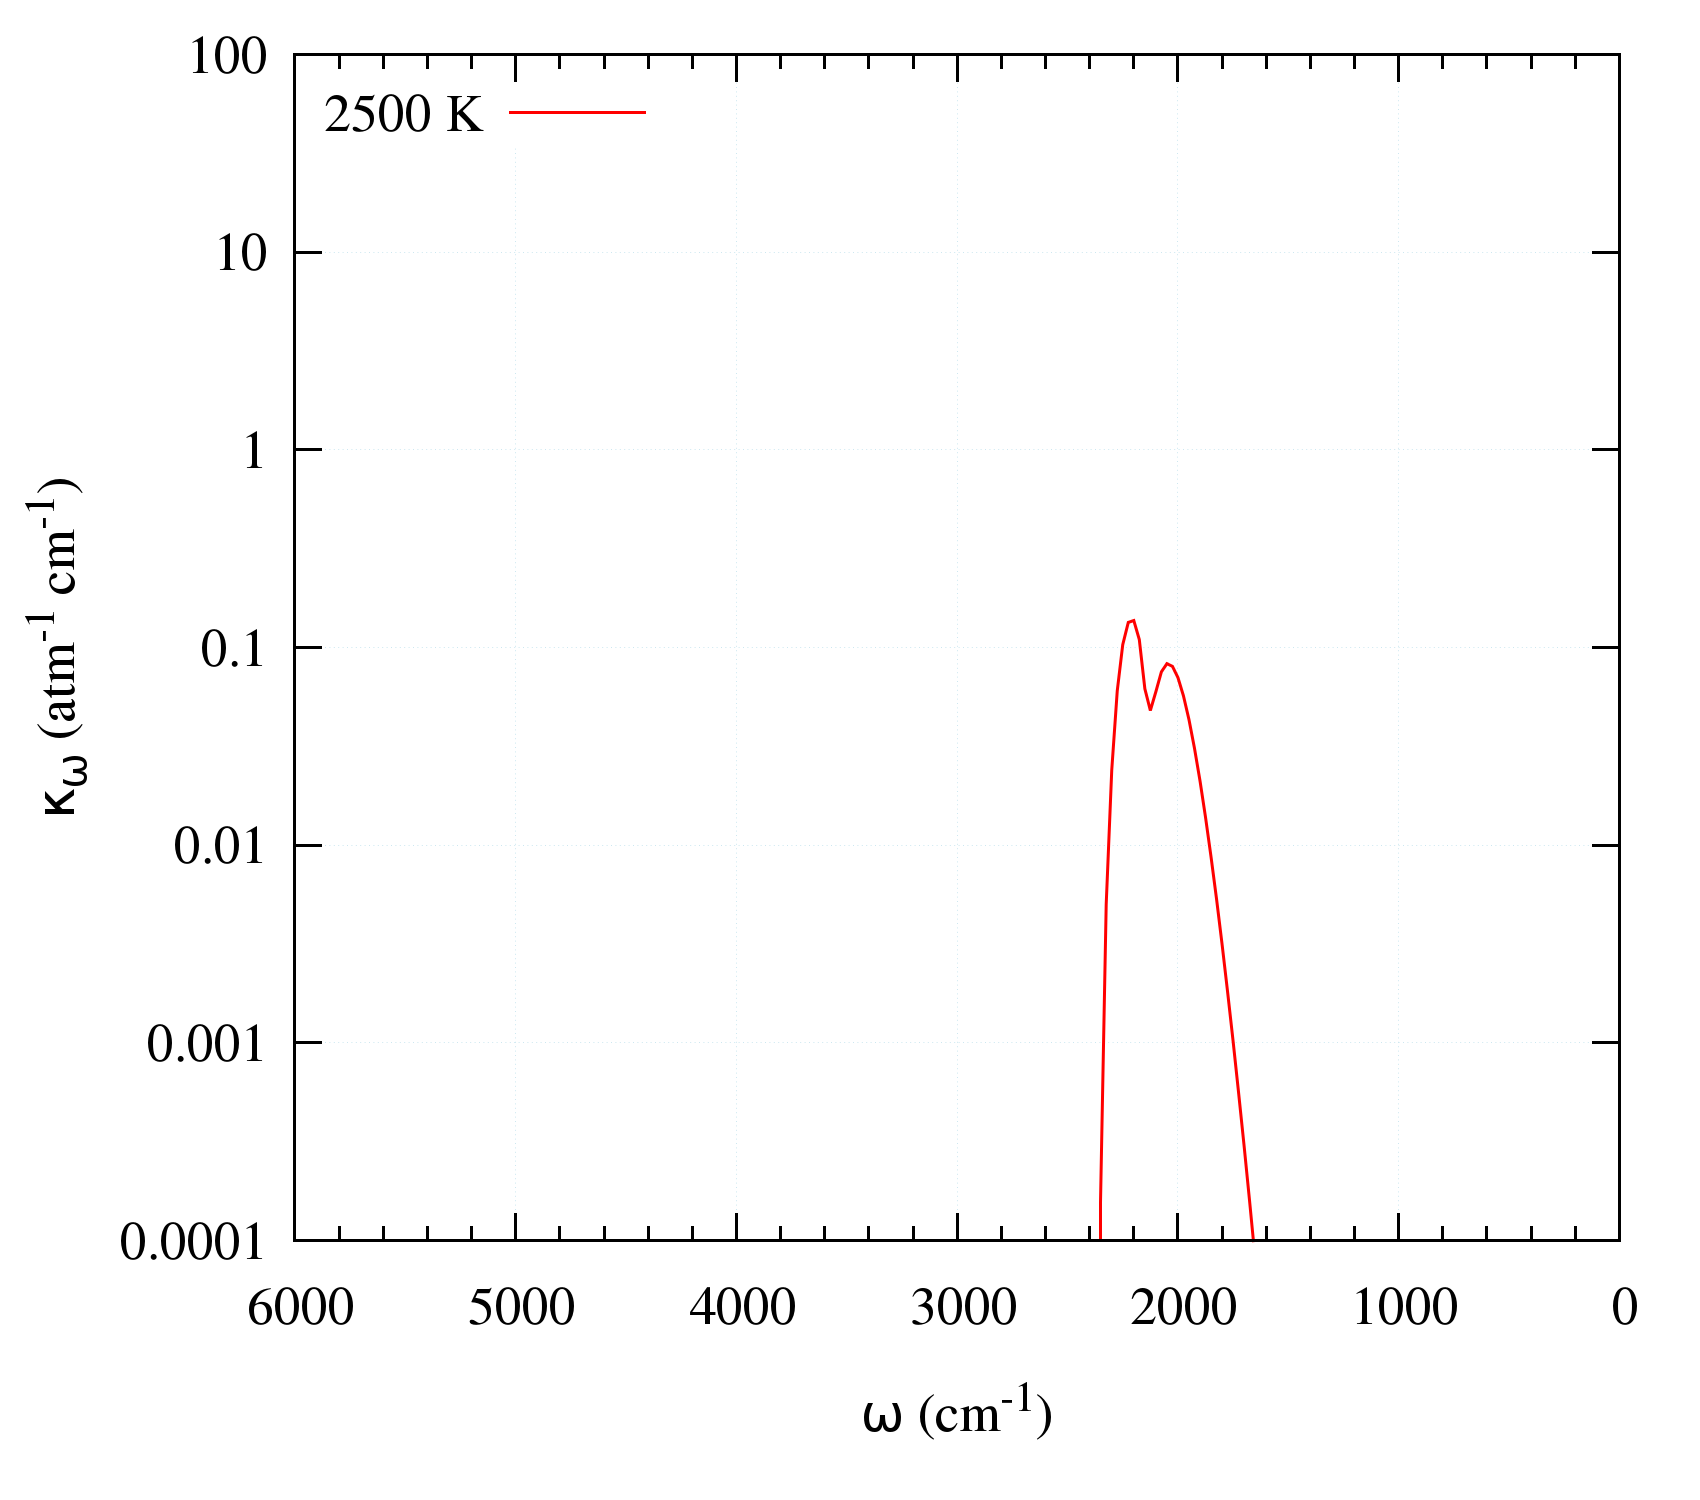
\includegraphics[height=2.5in]{Figures/CO_2500K.png} 
\end{tabular*}
\caption{Spectral variations of the CO mean absorption coefficient $\bar{\kappa}_{\om}$, in $\rm atm^{-1}.cm^{-1}$, at 300~K and 2500~K as tabulated in RadCal.\label{fig:CO_300-2500K}}
\end{figure}

The first overtone (centered at $ \om\approx 4260\;\rm {cm^{-1}}$) is not accounted for as its integrated band intensity is negligible at standard temperature and pressure. See Table \ref{Table::CO}. At 295~K, the integrated band intensity of Band~1 is $260\;\rm {atm^{-1}cm^{-2}}$. The statistical narrow band model associated with $\rm CO$ is the Goody model. Recommended temperatures of use range from 295~K to 2500~K.

\begin{table}[ht]
      \centering
      \caption{Spectral bands of $\rm CO$ included in RadCal.}
      \label{Table::CO}
    \begin{tabular}{|c|c|c|c|c|c|}
    \hline
    Band \# & \multicolumn{2}{|l|}{Bounds (cm$\rm ^{-1}$) } & Method & Assignment & $\alpha(T=296 \; {\rm K}) \; (\rm {atm^{-1} cm^{-2}})$   \\
    \cline{1-6}
    1 & 1600 & 2400 & modeled &  $\rm C\equiv O$ stretching & 260  \\
    \hline
   \end{tabular}
\end{table}


\clearpage

\section{Methane: $\rm CH_4$}

Methane is a spherical top molecule of tetrahedral shape with the carbon atom occupying the center of the tetrahedron. It belongs to the point group $T_d$. The methane IR spectrum is the result of the vibration-rotation modes of the $\rm C-H$ groups. It has nine vibrational modes, but due to its symmetry, this translates into only two distinct IR active fundamental vibration frequencies. In RadCal, the methane IR spectrum is divided into three distinct bands, which include the fundamentals plus degenerate (overtone) vibration modes. Bands 1 and 2 are calculated using tabulated mean absorption coefficient data which were obtained by Brosmer and Tien, \cite{Brosmer1985} for temperatures of 290, 600, 850~K. Band 3 is modeled, using a just-overlapping line model; the integrated intensities are computed in the harmonic-oscillator, rigid-rotator approximation. See Penner and Gray, Ref.~\cite{Gray1965}, for more details. In RadCal, the Elsasser model is used to calculate the collision optical depth. Table \ref{Table::CH4} tabulates the different characteristics of the $\rm CH_4$ bands.

\begin{table}[ht]
      \centering
      \caption{Spectral bands of $\rm CH_4$ included in RadCal.}
      \label{Table::CH4}
    \begin{tabular}{|c|c|c|c|c|c|}
    \hline
    Band \# & \multicolumn{2}{|l|}{Bounds (cm$\rm ^{-1}$) } & Method & Assignment & $\alpha(T=296 \; {\rm K}) \; (\rm {atm^{-1} cm^{-2}})$   \\
    \cline{1-6}
    1 & 1150 & 1600 & tabulated &  $\rm C-H$ Bend    & 237  \\
    2 & 2700 & 3250 & tabulated &  $\rm C-H$ Stretch & 212  \\
    3 & 3400 & 5000 & modeled   &  $\rm C-H$ Stretch &  35  \\
    \hline
   \end{tabular}
\end{table}
The strongest bands are Bands~1 and 2 which at standard temperature and pressure have an integrated band intensity of $237\;\rm {atm^{-1}cm^{-2}}$ and $212\;\rm {atm^{-1}cm^{-2}}$, respectively. Figure~\ref{fig:CH4_290-850K} displays the spectral mean absorption coefficient $\bar{\kappa}$ for $\rm CH_4$ at 290~K, 600~K, and 850~K, respectively.

\begin{figure}[ht]
\begin{tabular*}{\textwidth}{l@{\extracolsep{\fill}}r}
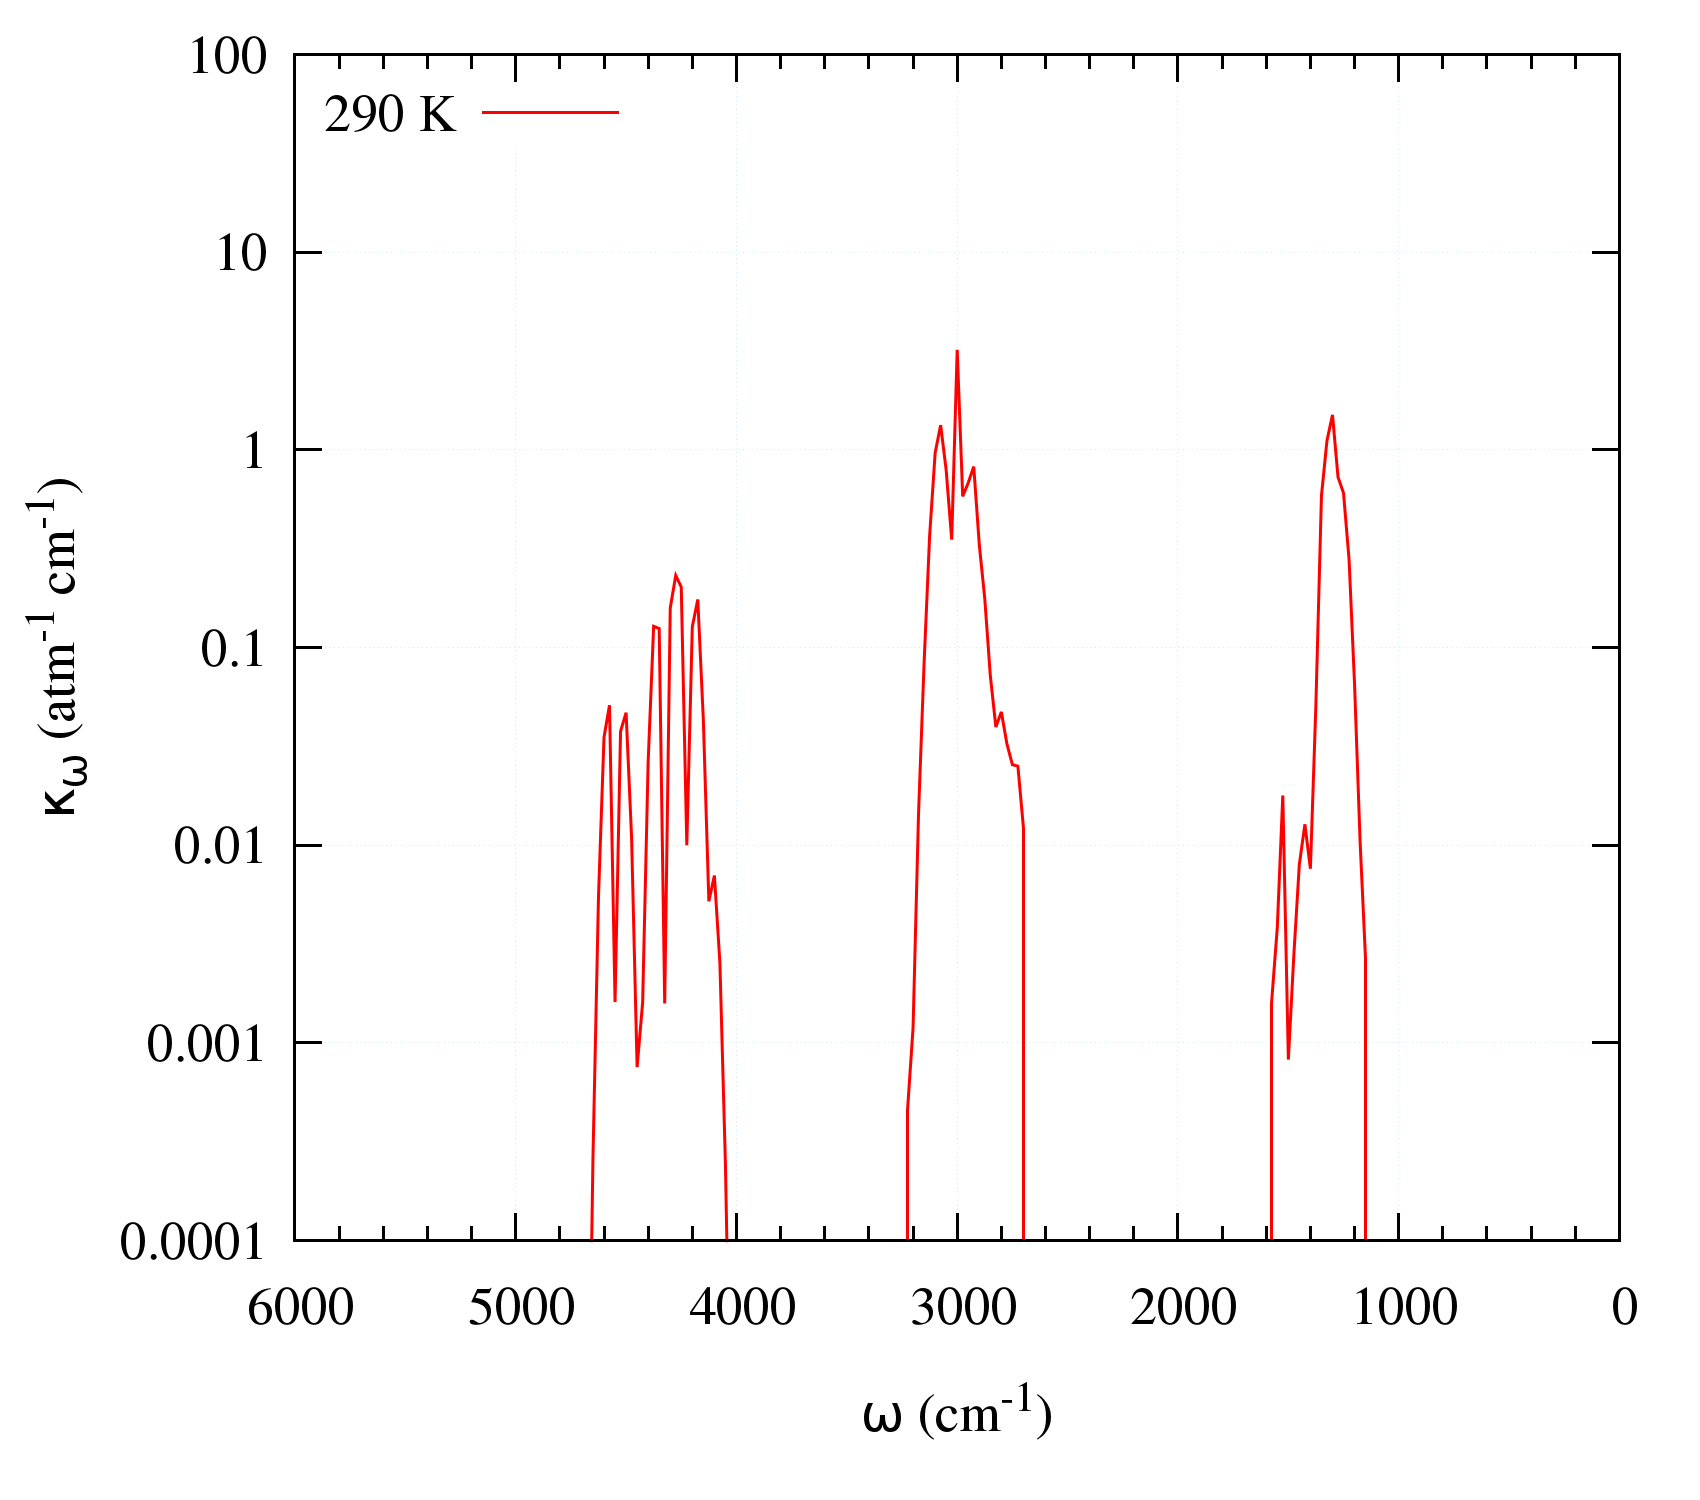
\includegraphics[height=2.5in]{Figures/CH4_290K.png} &
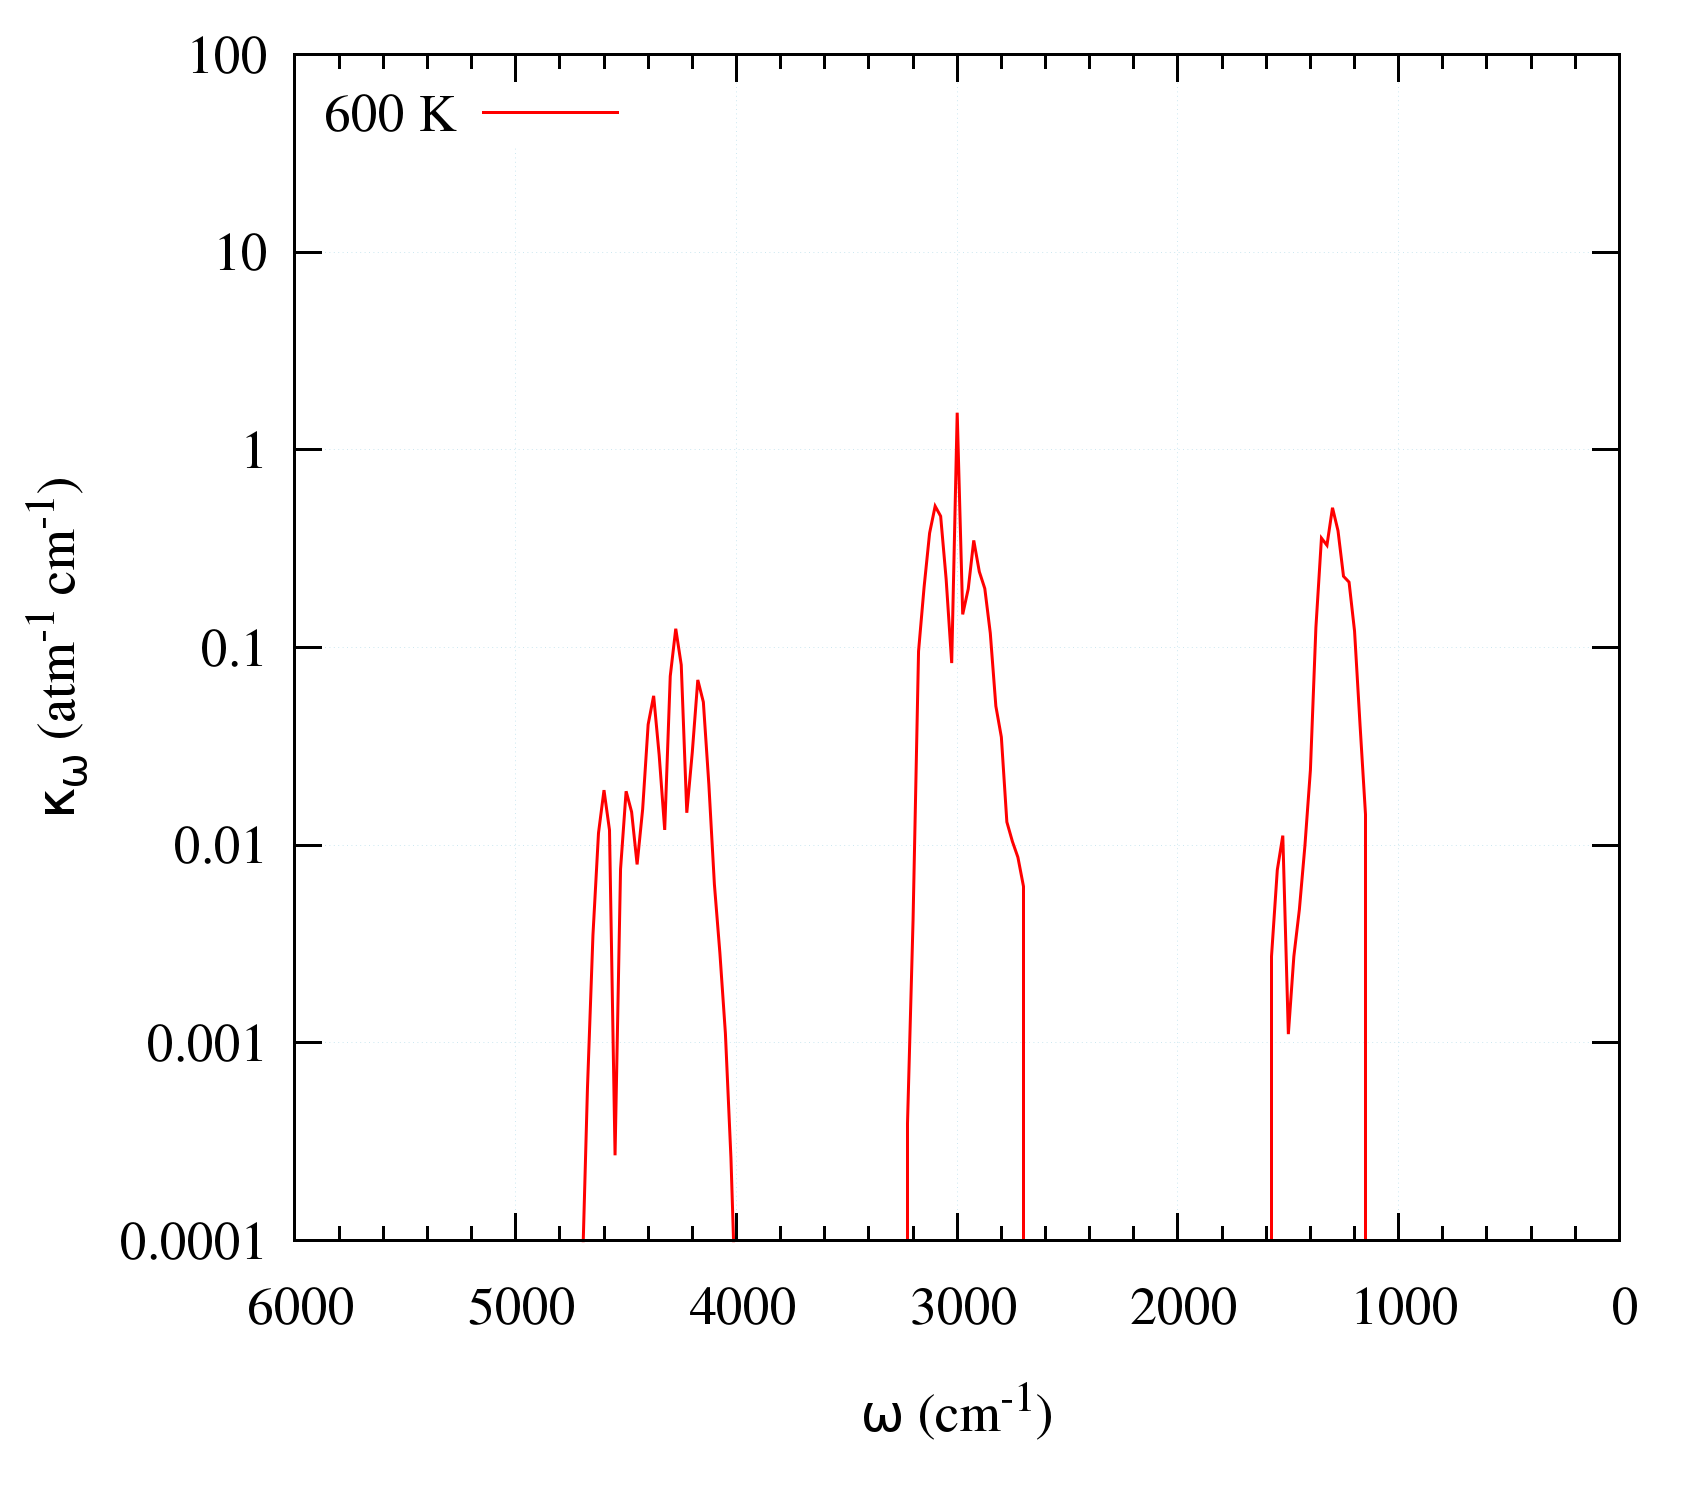
\includegraphics[height=2.5in]{Figures/CH4_600K.png} \\
\multicolumn{2}{c}{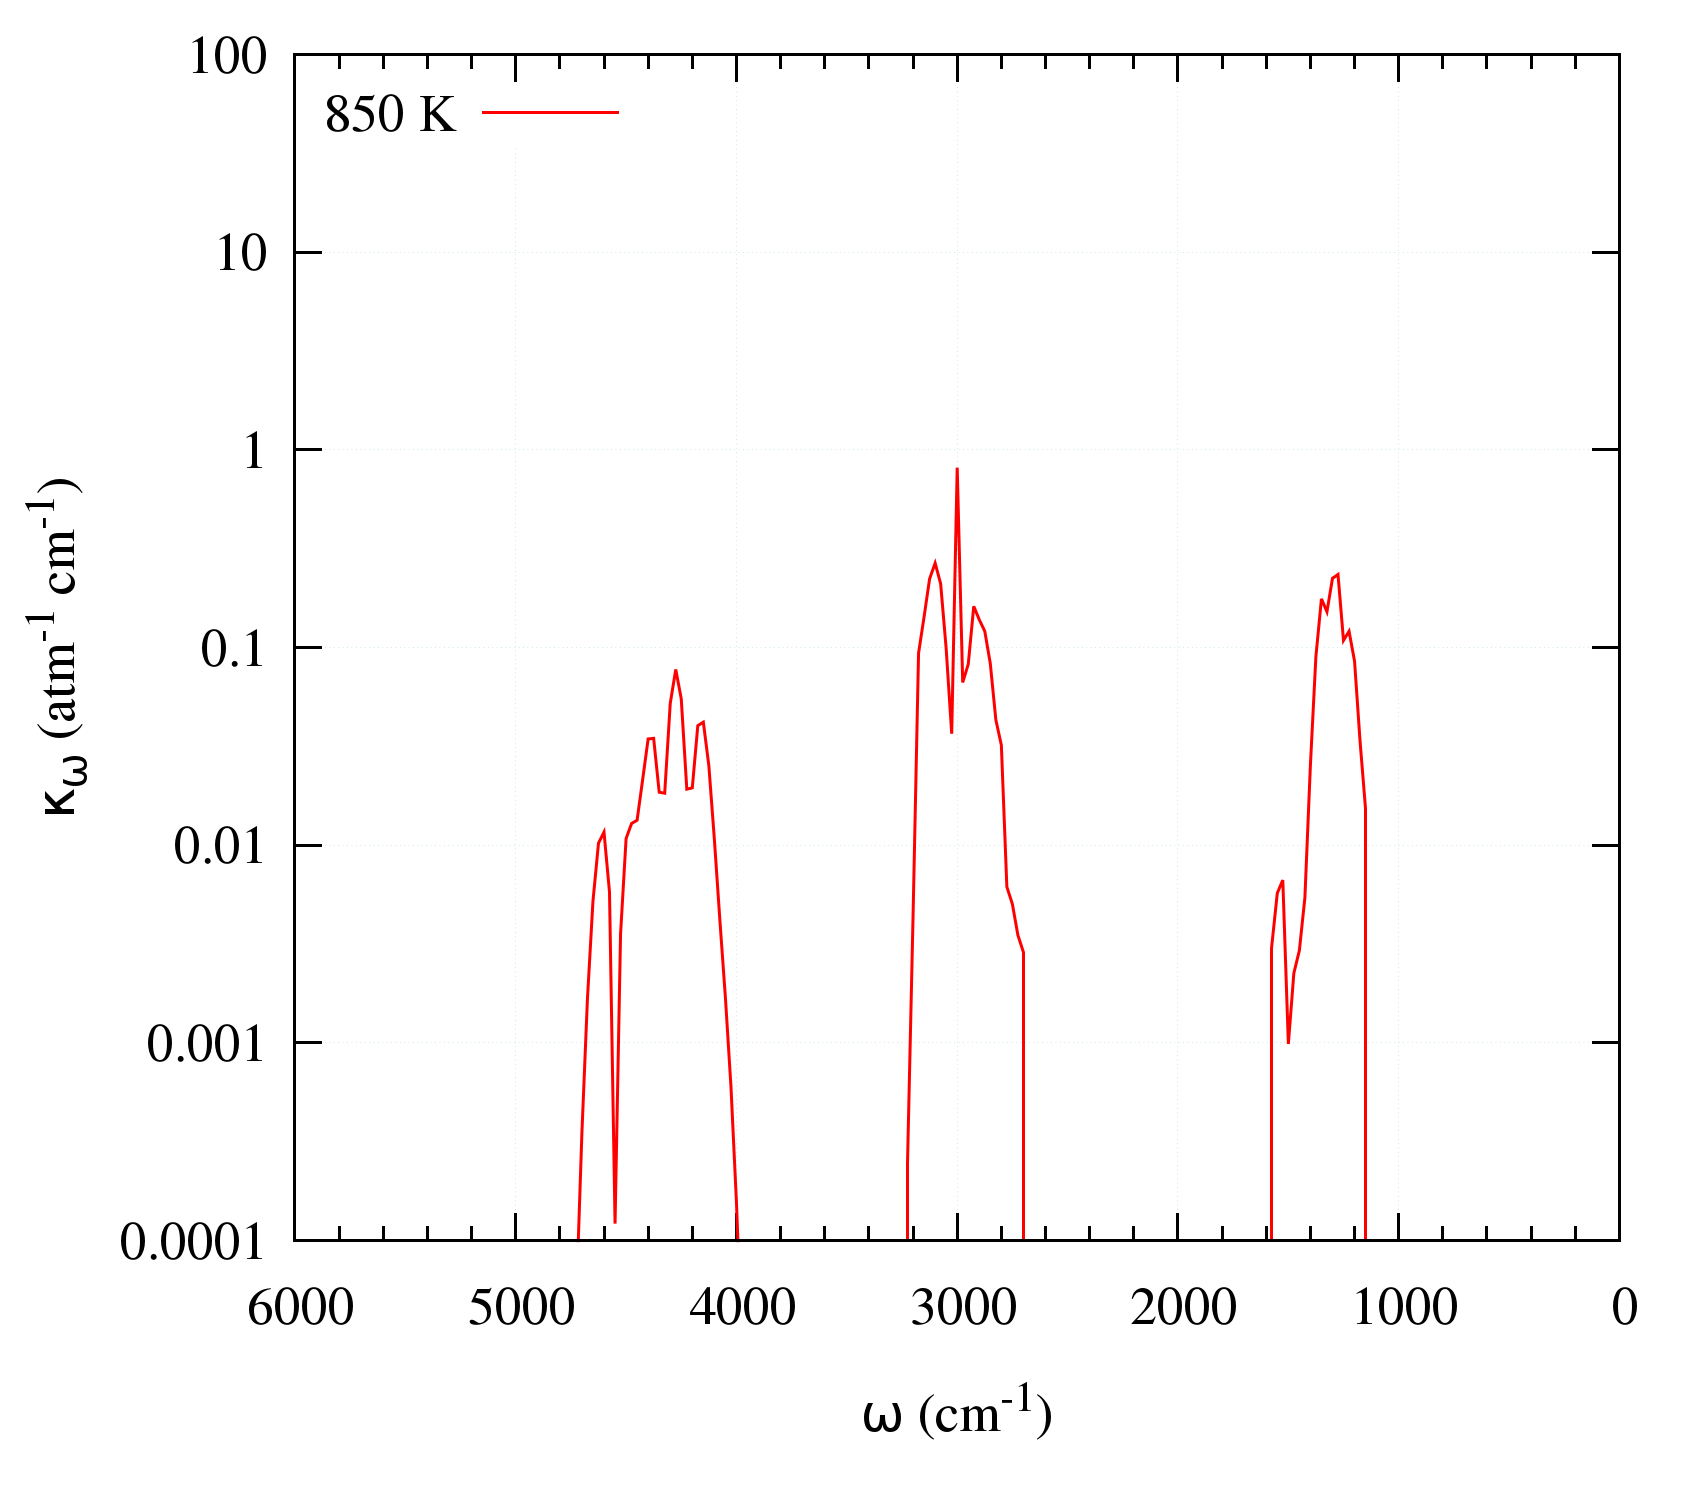
\includegraphics[height=2.5in]{Figures/CH4_850K.png}}
\end{tabular*}
\caption{Spectral variations of the $\rm CH_4$ mean absorption coefficient $\bar{\kappa}_{\om}$, in $\rm atm^{-1}.cm^{-1}$, at various temperatures as tabulated in RadCal.\label{fig:CH4_290-850K}}
\end{figure}

\clearpage

\section{Soot}

The soot spectral absorption coefficient is calculated using the below formulation:
\be\label{eq:soot_kappa}
\bar{\kappa} = 7.0 \om f_v
\ee
where $f_v$ is the soot volume fraction and is dimensionless. The narrow band transmissivity of soot is calculated as:
\be\label{eq::soot_optical_depth}
\bar{\tau}(0 \rightarrow s) = \exp\left(-\bar{\kappa} s \right).
\ee
From Eq.~\ref{eq:soot_kappa}, it can be seen that particulate matters tend to absorb soot in the high wavenumber part of the spectrum. Figure~\ref{fig:SOOT_300K} plots the spectral transmissivity of a homogeneous layer of soot at 300~K with a soot volume fraction value of 5~ppm ($5\times 10^{-6}$) and a thickness of 20~cm.

\begin{figure}[ht]
\begin{center}
 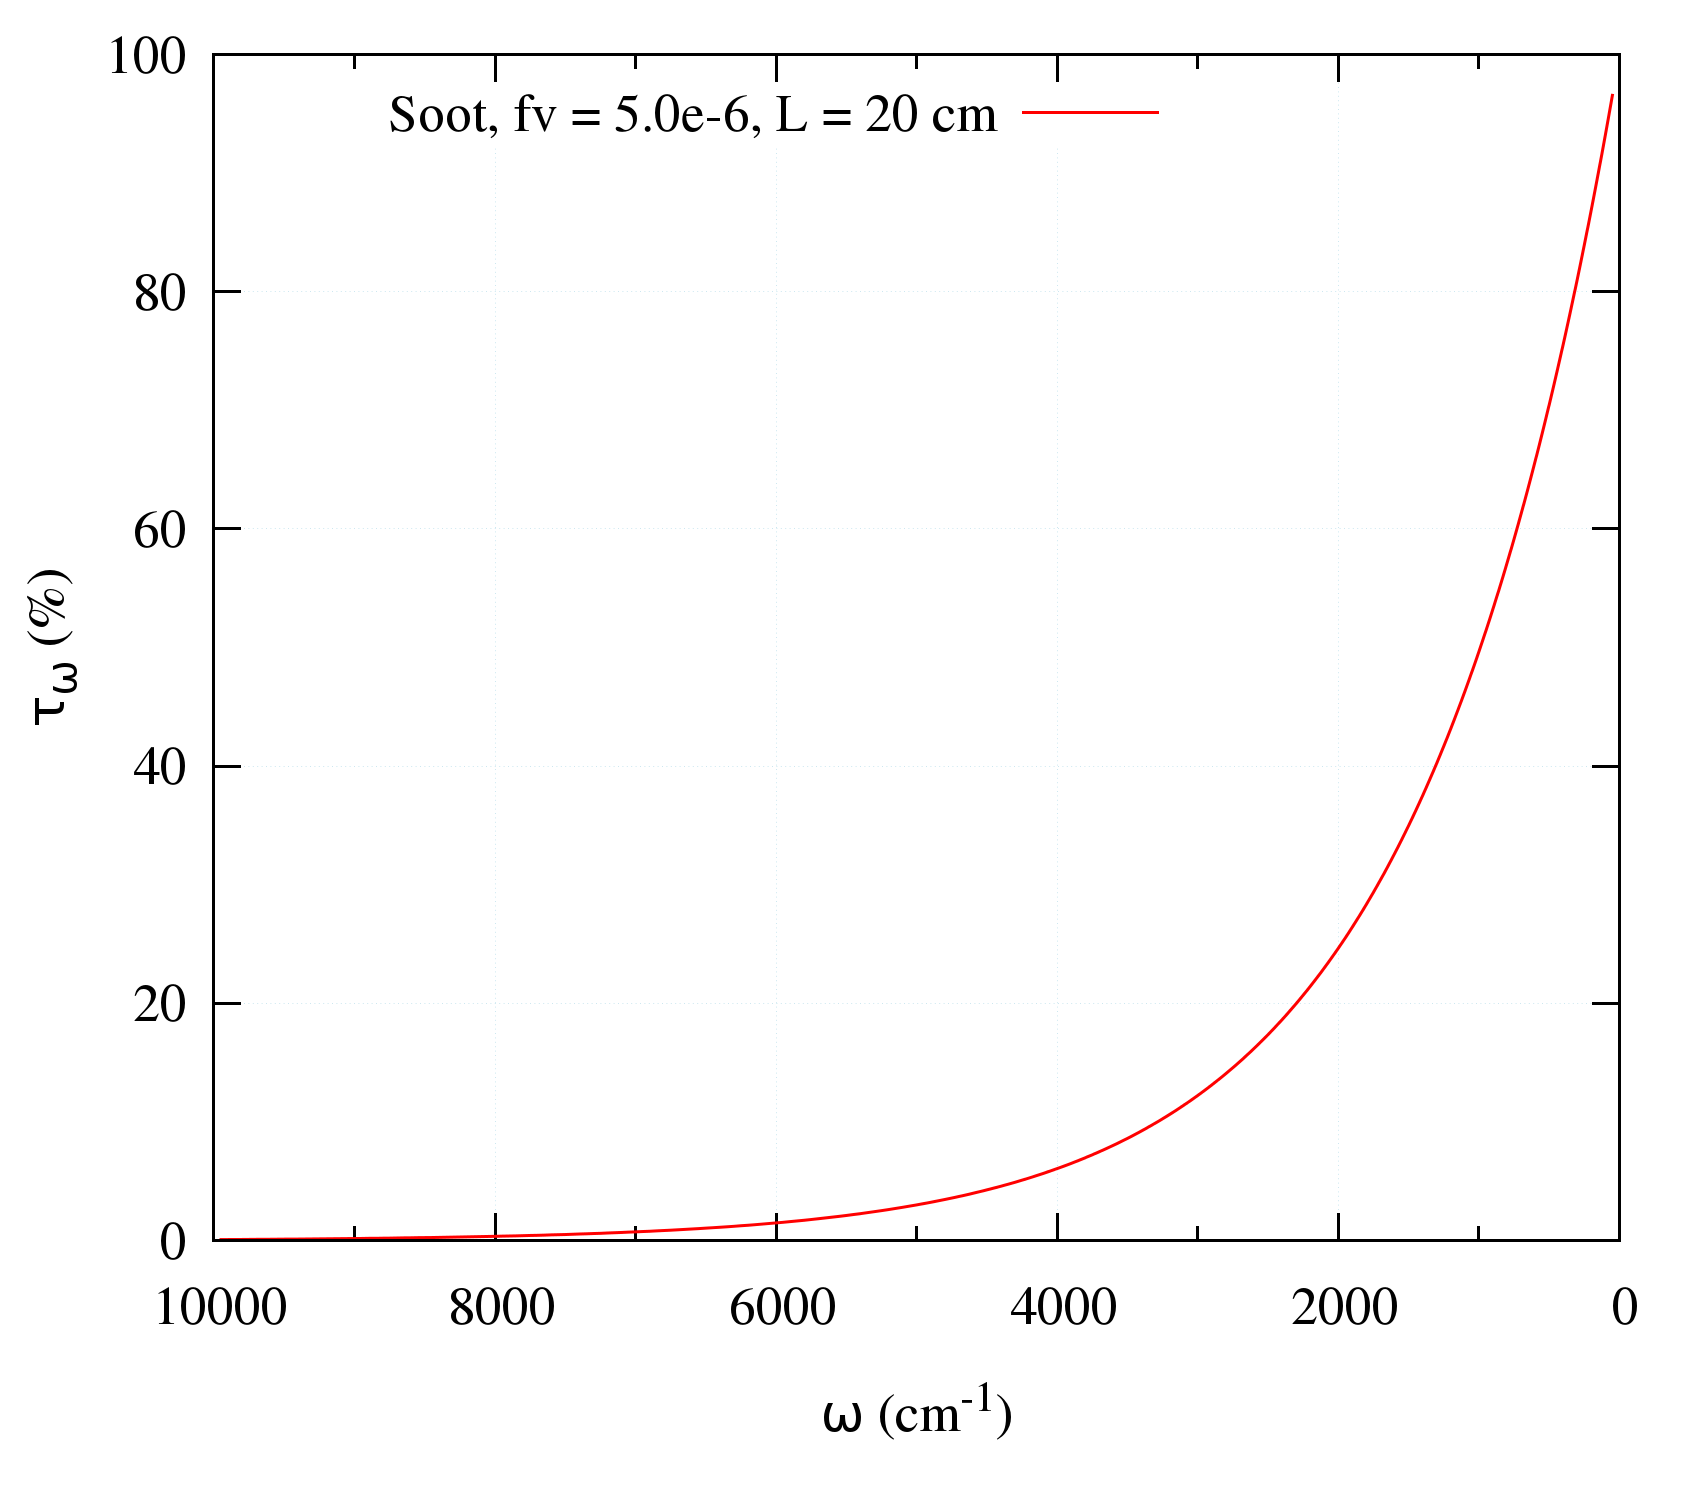
\includegraphics[height=2.5in]{Figures/SOOT_300K.png}
\end{center}
\caption{Predicted spectral transmissivity of a homogeneous layer of soot at 300~K, of thickness 20~cm, and with a soot volume fraction of 5~ppm ($f_v = 5\times 10^{-6}$).\label{fig:SOOT_300K}}
\end{figure}


\typeout{new file: New_Species_RadCal_Chapter.tex}

\chapter{The New Fuel Species in RadCal}
\label{chap:new_species}

The original RadCal data have been supplemented with new tabulated experimental data for the following fuels: Ethylene ($\rm C_2H_4$), Ethane ($\rm C_2H_6$), Propylene ($\rm C_3H_6$), Propane ($\rm C_3H_8$), Toluene ($\rm C_7H_8$), \textit{n}-Heptane ($\rm C_7H_{16}$), Methanol ($\rm CH_3OH$), Methyl Methacrylate ($\rm C_5H_8O_2$). These new data have been obtained through Wakatsuki Fourier Transform Infra-Red (FTIR) measurements for wavenumbers between 700--4000~cm$\rm ^{-1}$. See Ref.~\cite{Wakatsuki2005b} for a detailed description of the experimental methodology.

The sections below briefly describe the molecules and their IR active molecular bands. Bands bounds used in RadCal are tabulated with a brief description of the band assignment and their integrated band intensity (see definition below) at the lowest temperature is also included. Unlike the data previously included in RadCal that contained a mix of tabulated and modeled data, the species data presented here in the chapter are all tabulated.

\section{Integrated band intensity}
\label{sec:integrated_intensity}

A useful quantity to compare the relative importance of the different IR bands is provided by the integrated band intensity, $\alpha_i$, defined for the $i$th participating species as:
\be\label{eq:alpha}
  \alpha_i(T) = \displaystyle\int_{\om_{\min}}^{\om_{\max}} \bar{\kappa}_i(\om',T) \; \d \om'
\ee
whose units are $\rm {atm^{-1} cm^{-2}}$. The integrated band intensity is an intrinsic property of a molecule directly related to its geometry, its elements, and the nature of the chemical bonds. It is proportional to the amplitude of the electric moment variations for a vibration-rotation transition \cite{Matheson1932}. It is usually referred to as the coefficient $C_1$ in the exponential wide-band model.

The value of the spectral absorption coefficient, $\bar{\kappa}_i$, is averaged over a narrow band whose spectral width, $\Delta \om$, varies from 5~cm$^{-1}$ for $\om < $ 1100~cm$^{-1}$, to 25~cm$^{-1}$ for 1100~cm$^{-1} \leq \om < $ 5000~cm$^{\rm -1}$, and to 50~cm$^{\rm -1}$ for 5000~cm$^{\rm -1}\leq \om$. In the sections below, value were obtained by integrated the narrow band absorption coefficients over the band of interest.

\section{Fitting procedure}

In Section~\ref{Sec::SNBM}, expressions for the Elsasser, Goody, and Malkmus narrow band models were presented, see Eqs.~\ref{eq::Elsasser}, \ref{eq::Goody}, and \ref{eq::Malkmus}. Each gives a functional expression of the spectral transmissivity over narrow bands in the form:
\be
 \bar{\tau}_{\omega} = f(\bar{\kappa}_{\omega},\beta_{\omega},U),
\ee
where the expression of $f$ depends on the model chosen; the pressure-path $U =  P_i L$ is known from the experimental configuration; the experimental spectral transmissivity $\bar{\tau}_{\omega}$ is obtained by FTIR measurements; and the couple $\bar{\kappa}_{\omega},\beta_{\omega}$ are the sought parameters. In the following, the subscript $_\omega$ denoting the spectral dependence of the quantities is omitted for ease of reading.

To find the optimal narrow band model parameters for each model, at a given temperature and at a given wavenumber, a fitting objective function was minimized using a least-square fitting approach. The objective function $\mathcal{F}$ was defined as:
\be
 \mathcal{F}_i = \dfrac{|\bar{\tau}_{exp,i}-f(\bar{\kappa},\beta,U_i)|}{\bar{\tau}_{exp,i}},
\ee
where the subscript $_{exp}$ denotes experimentally measured values, and $_i$ denotes an experimental condition of  pressure-path. The experimental transmissivity relative to the $i^{th}$ pressure-path is denoted $\bar{\tau}_{exp,i}$. This is an averaged value over the narrow band interval at the desired resolution. Typically three different pressure-paths were used for each temperature and fuel. The narrow band parameters $\left(\bar{\kappa},\beta\right)$ hence found minimize the square of the \textit{l}$\rm ^2$-norm of the objective function $\mathcal{F}$:
\be
 \min\limits_{\left(\bar{\kappa},\beta\right)}\|\mathcal{F}\|_2^2 = \min\limits_{\left(\bar{\kappa},\beta\right)}\left(\displaystyle\sum \limits_i \left(\dfrac{\bar{\tau}_{exp,i}-f(\bar{\kappa},\beta,U_i)}{\bar{\tau}_{exp,i}}\right)^2\right).
\ee

The spectral narrow band parameters were obtained for all the fuels presented in this section, for the three aforementioned narrow band models. As a verification test, the experimental transmissivities obtained were reconstructed using the narrow band models and compared with the measured values. For each experimental condition, very good agreements were observed between the synthetic and the experimental transmissivity profiles regardless of the narrow band model. No model stands out nor performs better than the other two.

The similar accuracy of three different narrow band models is likely a result of the small number of pressure-paths used to fit the data;  the fitted narrow-band parameters were obtained by fitting only three experimental pressure-paths. In previous works, the appropriate band narrow band model was selected based on the value of the model deviation from the experimental data, see Ref.~\cite{Kunitomo1975}. This is an valid method as long as the experimental data has lower error than that associated with any narrow band models. Here, the experimental error associated with the mean absorption coefficient is 5\% \cite{Wakatsuki2008}, which is higher than the difference between experimental and synthetic data for each model.

It is customary to validate the choice of the assumed narrow band model or to derive its parameters from the knowledge of the integrated band intensities, $\alpha$, defined by Eq.~\ref{eq:alpha}. Experimentally, $\alpha$ is computed from the extrapolation technique first proposed by Wilson and Wells \cite{Wilson1946,Thorndike1947} and further explained in Penner~\cite{Penner1959}. The technique is briefly recalled. A parameter $B$ is defined as:
\be
 B = \dfrac{1}{P_iL} \displaystyle\int\limits_{band} -\ln(\tau_{\omega}) {\rm d} \omega.
\ee
The apparent integrated band intensity, $\mathcal{A}$, defined as:
\be
 \mathcal{A} = \displaystyle\int\limits_{band}{-\ln{\tau_{\omega}}} {\rm d} \omega
\ee
relates with $B$ through the relation:
\be
\label{eq:LineofGrowth}
\mathcal{A} = P_iL B.
\ee
The work by Wilson and Wells \cite{Wilson1946,Thorndike1947} showed that the $\alpha$ relates with the parameter $B$ through:
\be
\label{eq:Exp_alpha}
 \alpha = \lim\limits_{P_iL\rightarrow 0} B
\ee

Hence, the experimental value for $\alpha$ can be obtained through extrapolation of $A$ to the origin and
measuring the slope at the origin. While a direct extrapolation is not recommended as it may be subject to significant error as mentioned by Kaplan \textit{et al.}, \cite{Kaplan1956a}, a extrapolation using an educated curve-of-growth procedure \cite{Kaplan1956a} can help alleviate this problem. The functional relation between the absorption and the pressure-path can be assumed to be a function of the unknown $\alpha$ and some characteristic line width. Fitting the experimental data is required to obtain the unknown parameters and it provides a more rigorous evaluation of $\alpha$.

While a representative functional relation can be derived for a fundamental band, \textit{i.e.} a band associated with only one vibration transition mode, it is more difficult to do so for bands that are the results of multiple vibration modes. This is the case for all the species presented here. Hence, no extrapolation was performed as they could lead to bias depending on the extrapolation method used. Instead, following comments presented in Modest~\cite{Modest2013}, the Malkmus model was chosen as it is recognized as the best for polyatomic molecules. Verification tests for each species are presented in Section~\ref{sec:verification}. Some of the data, ethane, ethylene, and propane, have been carefully examined and some species were compared with the HITRAN 2012 edition. See Lecoustre \textit{et al.} \cite{Lecoustre2014} for more details.

\clearpage

\section{Ethylene: $\rm C_2H_4$}

\subsection{Integrated Band Intensity}

Ethylene, $\rm C_2H_4$, is a plane symmetrical molecule and belongs to the point group $D_{2h}$. It has 12 vibrational modes. In RadCal, its IR spectrum is divided into four distinct bands that are associated with different vibrational modes, see Table \ref{Table::C2H4}. The bands from 750 - 1250~cm$^{-1}$ and 1300 - 1600~cm$^{-1}$ are associated with the bending motion of the $\rm CH_2$ groups. The band between 1750 and 2075~cm$^{-1}$ is associated with the stretching motion of the carbon double bond, $\rm C=C$. The fourth band from 2800 - 3400~cm$^{-1}$ is associated with the stretching of the CH groups. The strongest absorption band is located at lower wavenumbers, between 780 and 1250~cm$^{-1}$. This indicates the propensity of ethylene to strong participation to the radiative heat exchange corresponding to low to moderate temperatures. This spectral range corresponds to the highest blackbody spectral emittance at temperatures ranging between 400 to 700~K which are characteristic of cooler regions of the fuel rich cores for liquid and solid fires.
\begin{table}[ht]
    \centering
    \caption{Spectral bands of $\rm C_2H_4$ included in RadCal.}
    \vspace{0.1in}
    \label{Table::C2H4}
    \begin{tabular}{|c|c|c|c|c|}
      \hline
      Band \# & \multicolumn{2}{|l|}{Bounds (cm$\rm ^{-1}$) } & Assignment & $\alpha(T=296 \; {\rm K}) \; (\rm {atm^{-1} cm^{-2}})$\\
      \cline{1-5}
      1 & 750  & 1250 &  $\rm CH_2$ Bend      & 371 \\
      2 & 1300 & 1600 &  $\rm CH_2$ Bend      & 42  \\
      3 & 1750 & 2075 &  $\rm C=C$  Stretch   & 20  \\
      4 & 2800 & 3400 &  $\rm C-H$  Stretch   & 198 \\
      \hline
    \end{tabular}
\end{table}
Band~1 is the strongest absorbing band. All the ethylene IR spectral absorption data were obtained from high resolution FTIR experiments with temperatures varying from 296~K to 1000~K. See Wakatsuki \cite{Wakatsuki2005b} for more details about the experimental process followed to obtain the experimental data.

\subsection{Malkmus Narrow Band Parameters}

The spectral absorption coefficients were obtained by least square fitting of the experimental transmissivity using the Malkmus model. The ethylene narrow band parameters, $\bar{\kappa}$ and $\beta$, for temperatures ranging from 296~K to 1000~K are plotted in Figures~\ref{fig:ethylene_kappa_beta1}--\ref{fig:ethylene_kappa_beta4} for Bands 1 to 4.

\newpage

\begin{figure}[p]
\begin{center}
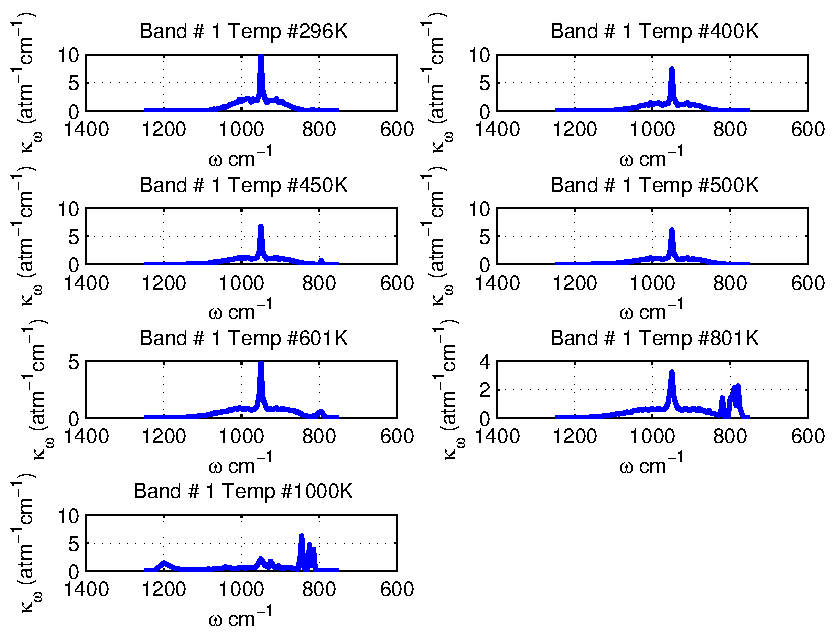
\includegraphics[width=5.0in]{Figures/Ethylene_Kappa_Band1_MALKMUS.pdf}
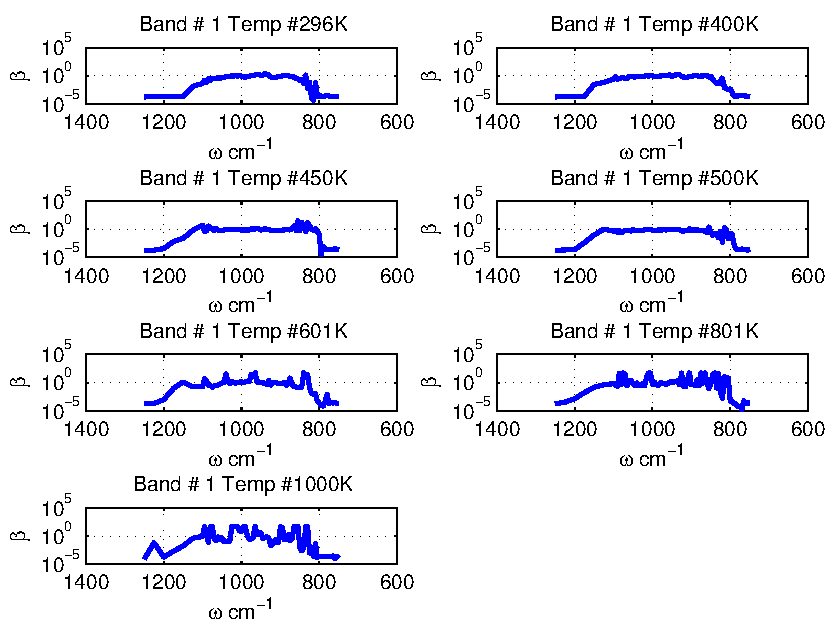
\includegraphics[width=5.0in]{Figures/Ethylene_Beta_Band1_MALKMUS.pdf}
\end{center}
\caption{Ethylene narrow band parameters $\bar{\kappa}$ and $\beta$ obtained for the 750--1250~cm$^{-1}$ band corresponding to the bending motion of the $\rm CH_2$ chemical group. Temperatures plotted are: 296, 400, 450, 500, 601, 801, and 1000~K. The narrow band resolution $\Delta \om$ is 5~cm$^{-1}$.\label{fig:ethylene_kappa_beta1}}
\end{figure}

\begin{figure}[p]
\begin{center}
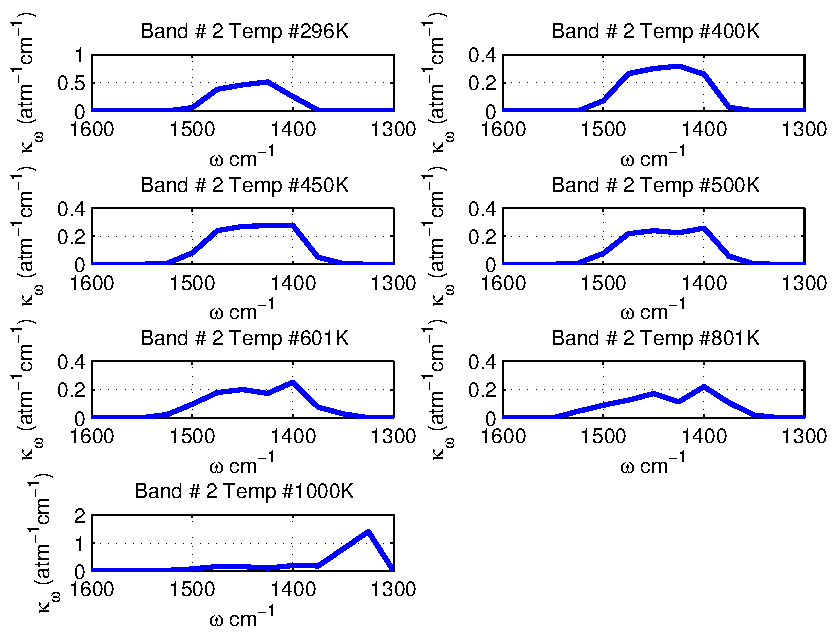
\includegraphics[width=5.0in]{Figures/Ethylene_Kappa_Band2_MALKMUS.pdf}
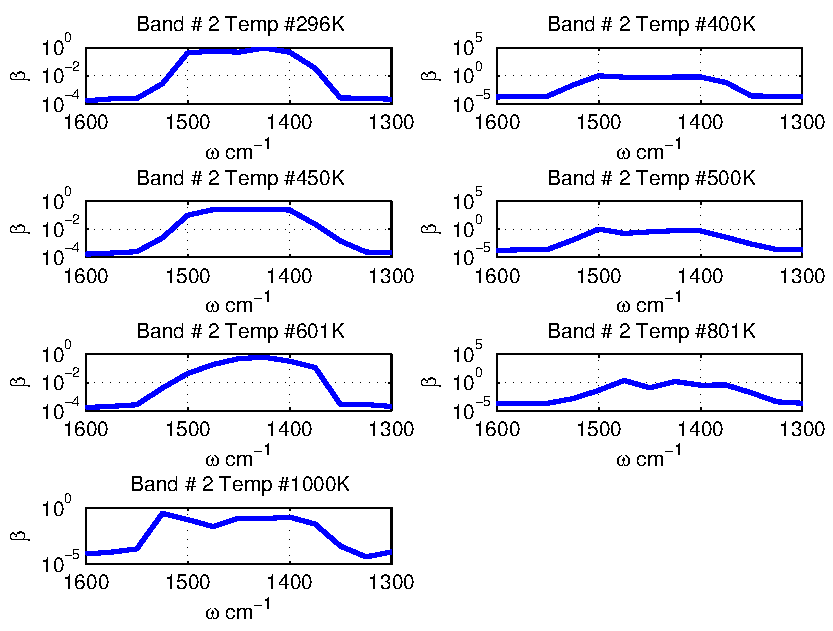
\includegraphics[width=5.0in]{Figures/Ethylene_Beta_Band2_MALKMUS.pdf}
\end{center}
\caption{Ethylene narrow band parameters $\bar{\kappa}$ and $\beta$ obtained for the 1300--1600~cm$^{-1}$ band corresponding to the bending motion of the $\rm CH_2$ chemical group. Temperatures plotted are: 296, 400, 450, 500, 601, 801, and 1000~K. The narrow band resolution $\Delta \om$ is 25~cm$^{-1}$.\label{fig:ethylene_kappa_beta2}}
\end{figure}

\begin{figure}[p]
\begin{center}
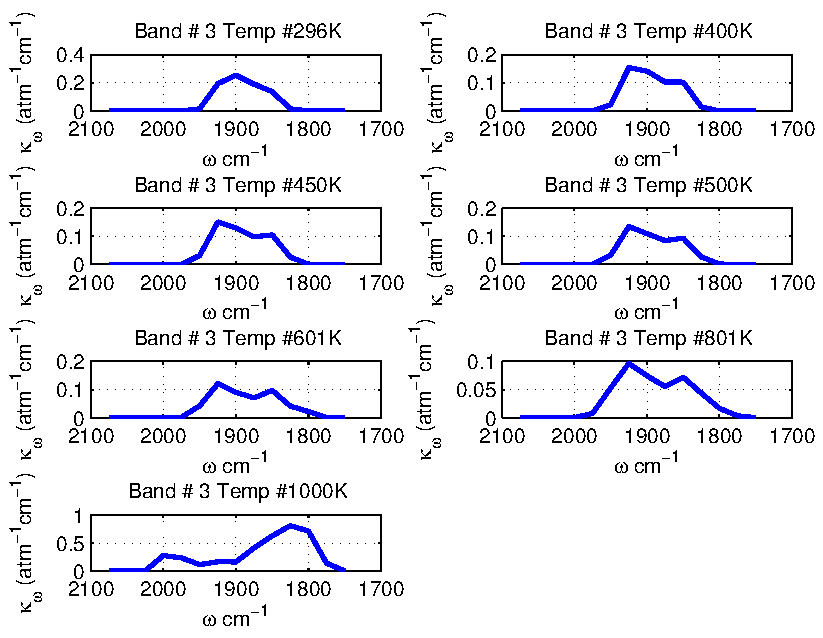
\includegraphics[width=5.0in]{Figures/Ethylene_Kappa_Band3_MALKMUS.pdf}
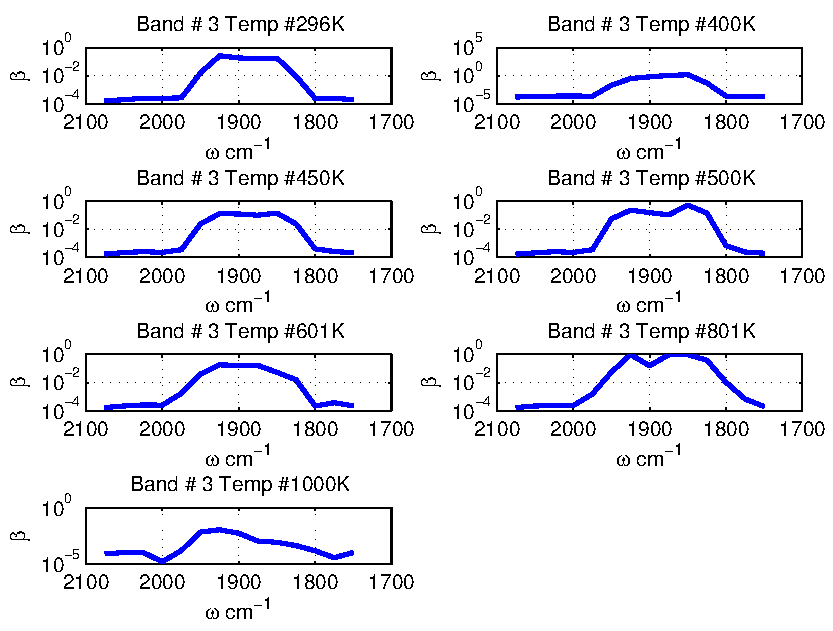
\includegraphics[width=5.0in]{Figures/Ethylene_Beta_Band3_MALKMUS.pdf}
\end{center}
\caption{Ethylene narrow band parameters $\bar{\kappa}$ and $\beta$ obtained for the 1750--2075~cm$^{-1}$ band corresponding to the stretching motion of the $\rm C=C$ chemical group. Temperatures plotted are: 296, 400, 450, 500, 601, 801, and 1000~K. The narrow band resolution $\Delta \om$ is 25~cm$^{-1}$.\label{fig:ethylene_kappa_beta3}}
\end{figure}

\begin{figure}[p]
\begin{center}
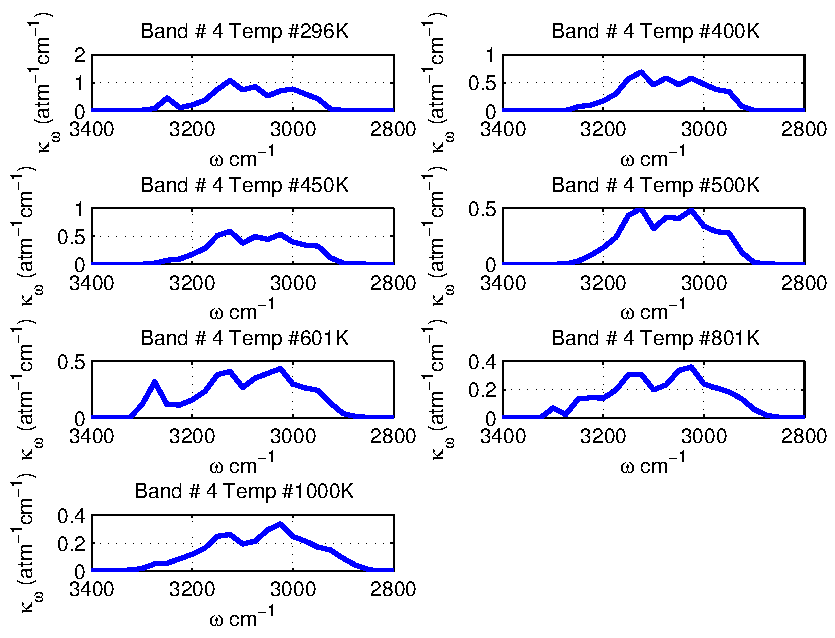
\includegraphics[width=5.0in]{Figures/Ethylene_Kappa_Band4_MALKMUS.pdf}
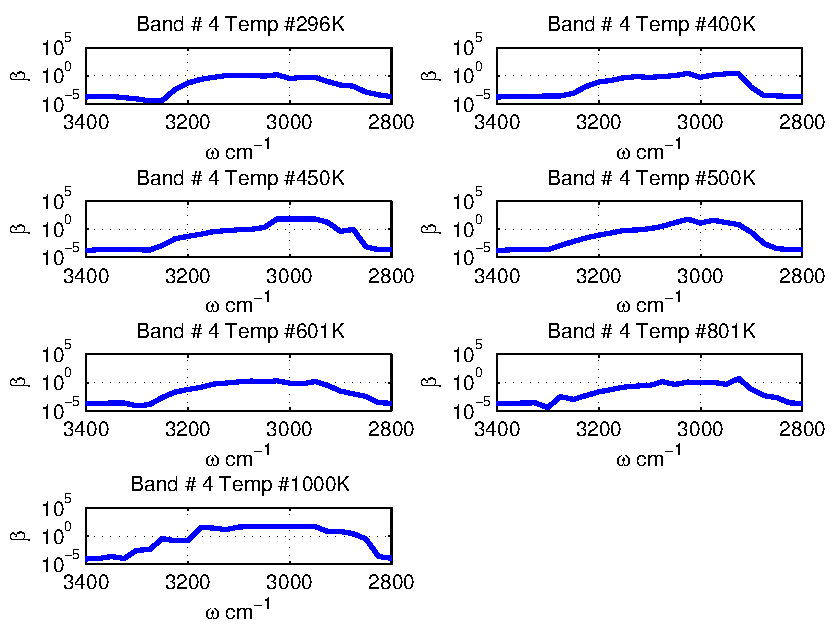
\includegraphics[width=5.0in]{Figures/Ethylene_Beta_Band4_MALKMUS.pdf}
\end{center}
\caption{Ethylene narrow band parameters $\bar{\kappa}$ and $\beta$ obtained for the 2800--3400~cm$^{-1}$ band corresponding to the stretching motion of the $\rm C-H$ chemical group. Temperatures plotted are: 296, 400, 450, 500, 601, 801, and 1000~K. The narrow band resolution $\Delta \om$ is 25~cm$^{-1}$.\label{fig:ethylene_kappa_beta4}}
\end{figure}

\FloatBarrier

\subsection{Verification SNB Parameters}

To assess the accuracy of the narrow band parameters $\bar{\kappa}$ and $\beta$, synthetic transmissivities were constructed for the same experimental conditions as the FTIR data and compare with it. This subsection plots the comparison and the relative error in transmissivity (relative to FTIR measurements) using the ethylene parameters presented in Figs.~\ref{fig:ethylene_kappa_beta1} to \ref{fig:ethylene_kappa_beta4}.


\begin{figure}[!h]
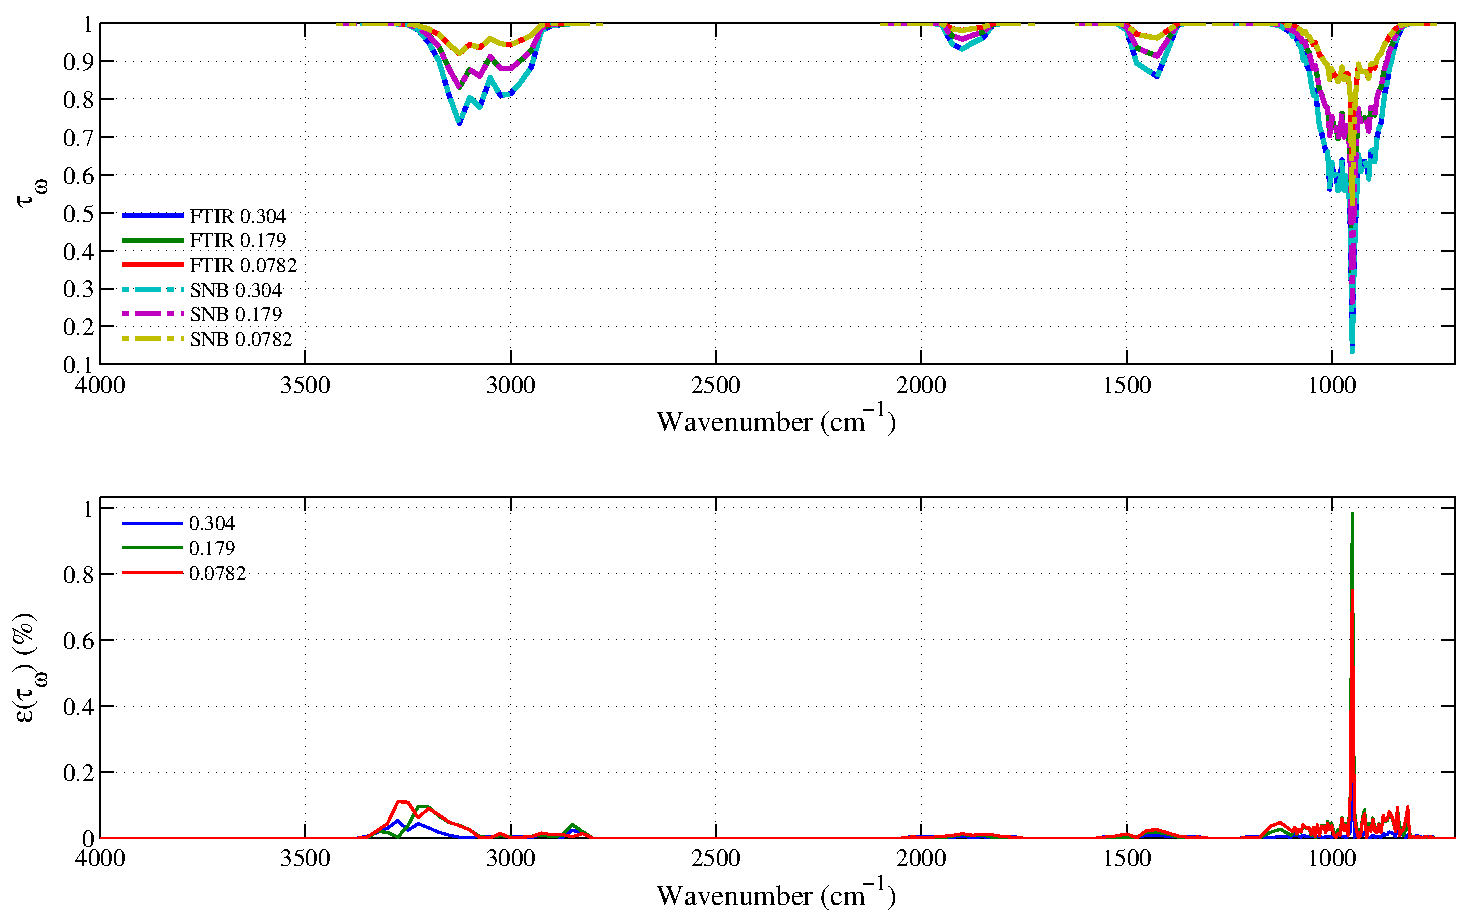
\includegraphics[width=\textwidth]{Figures/Comparison_Fit_Ethylene_MALKMUS_Temp296K.pdf}
\caption{Top: comparison between the experimental (FTIR, in solid lines) and the synthetic (dashed lines) spectral transmissivity profiles, denoted $\tau_{\omega}$, of an isothermal homogeneous column of ethylene. The synthetic profiles was generated using the Malkmus narrow band parameters presented in Figs.~\ref{fig:ethylene_kappa_beta1} to \ref{fig:ethylene_kappa_beta4}. Bottom: relative transmissivity error, denoted $\epsilon{(\tau_{\omega})}$, between the experiment and the synthetic profiles presented on the top figure. Three different pressure-paths are considered: 0.304, 0.179 and 0.0782 atm.cm. The gas temperature is set at 296~K and the total pressure is 101 kPa. Note: the experimental data resolution has been changed to match that of the narrow band model. \label{fig:ethylene_SNBVerify_296K}}
\end{figure}

\begin{figure}[p]
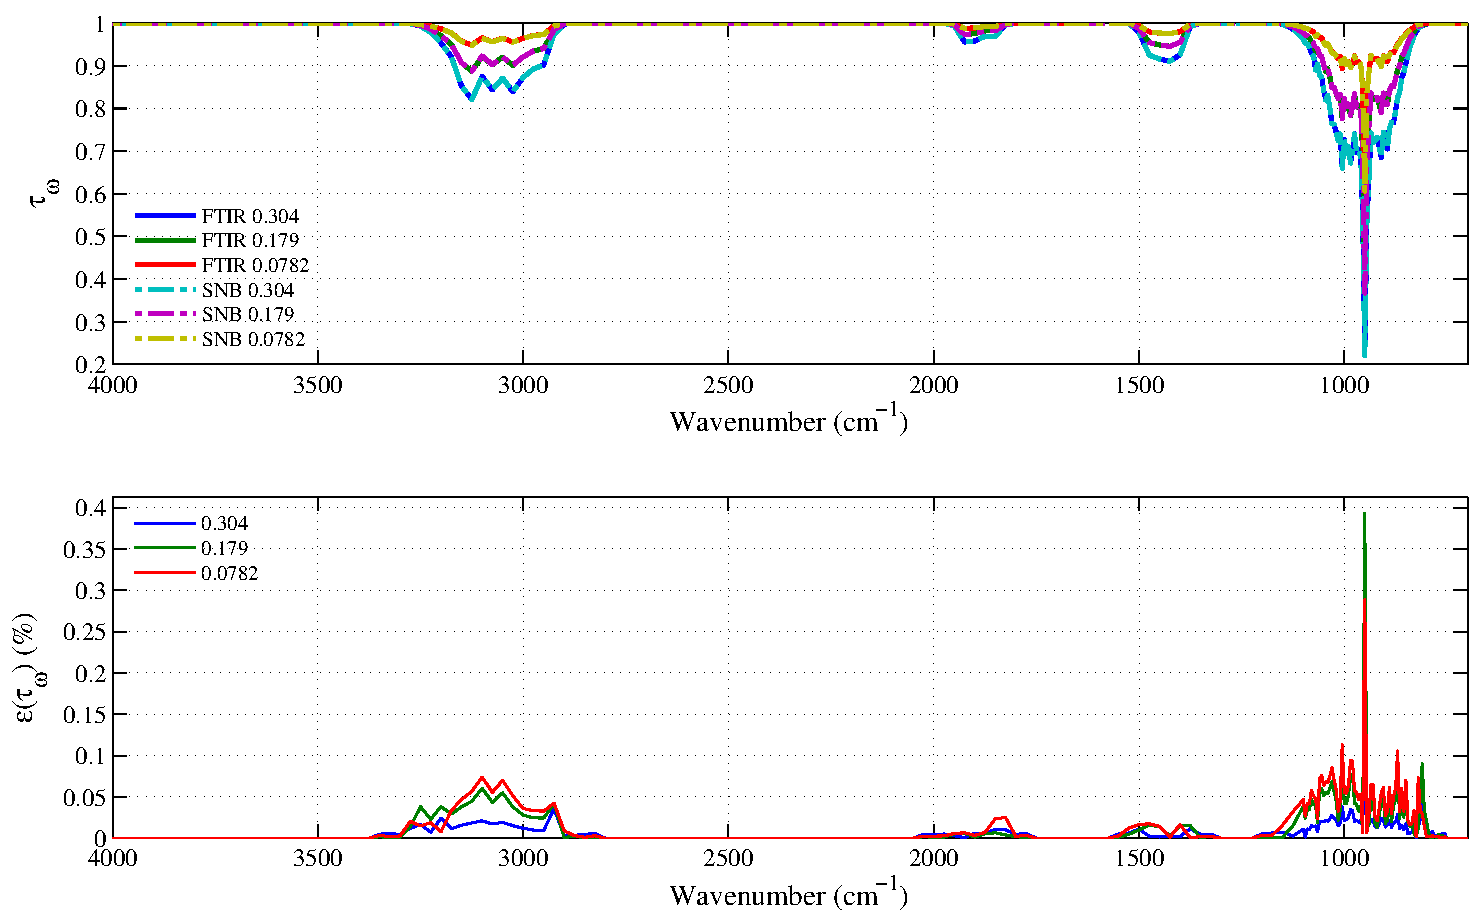
\includegraphics[width=\textwidth]{Figures/Comparison_Fit_Ethylene_MALKMUS_Temp400K.pdf}
\caption{Top: comparison between the experimental (FTIR, in solid lines) and the synthetic (dashed lines) spectral transmissivity profiles, denoted $\tau_{\omega}$, of an isothermal homogeneous column of ethylene. The synthetic profiles was generated using the Malkmus narrow band parameters presented in Figs.~\ref{fig:ethylene_kappa_beta1} to \ref{fig:ethylene_kappa_beta4}. Bottom: relative transmissivity error, denoted $\epsilon{(\tau_{\omega})}$, between the experiment and the synthetic profiles presented on the top figure. Three different pressure-paths are considered: 0.304, 0.179 and 0.0782 atm.cm. The gas temperature is set at 400~K and the total pressure is 101 kPa. Note: the experimental data resolution has been changed to match that of the narrow band model. \label{fig:ethylene_SNBVerify_400K}}
\end{figure}

\begin{figure}[p]
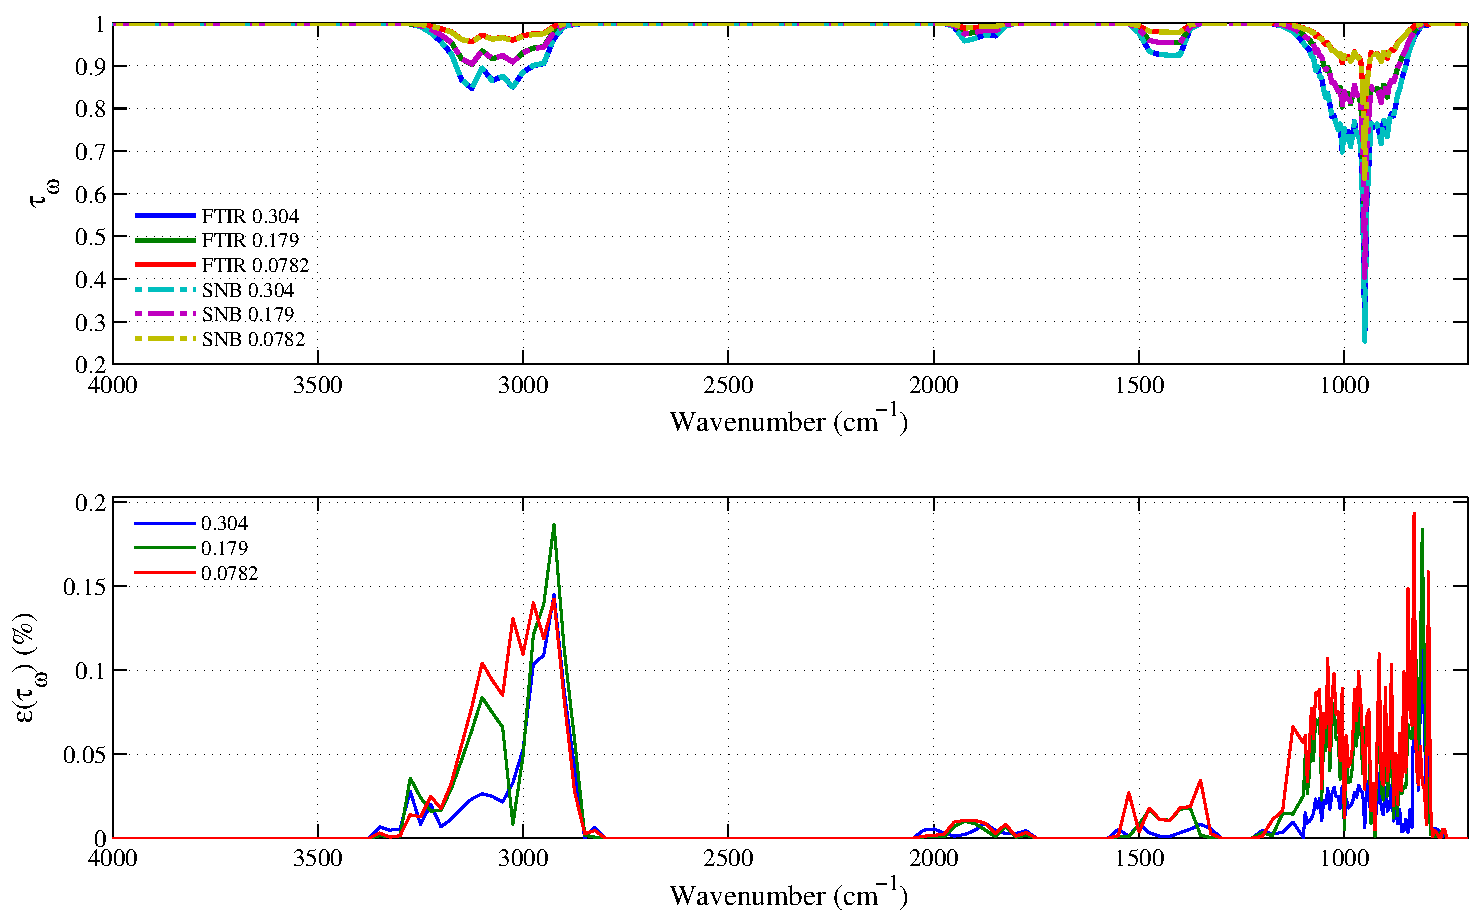
\includegraphics[width=\textwidth]{Figures/Comparison_Fit_Ethylene_MALKMUS_Temp450K.pdf}
\caption{Top: comparison between the experimental (FTIR, in solid lines) and the synthetic (dashed lines) spectral transmissivity profiles, denoted $\tau_{\omega}$, of an isothermal homogeneous column of ethylene. The synthetic profiles was generated using the Malkmus narrow band parameters presented in Figs.~\ref{fig:ethylene_kappa_beta1} to \ref{fig:ethylene_kappa_beta4}. Bottom: relative transmissivity error, denoted $\epsilon{(\tau_{\omega})}$, between the experiment and the synthetic profiles presented on the top figure. Three different pressure-paths are considered: 0.304, 0.179 and 0.0782 atm.cm. The gas temperature is set at 450~K and the total pressure is 101 kPa. Note: the experimental data resolution has been changed to match that of the narrow band model. \label{fig:ethylene_SNBVerify_450K}}
\end{figure}

\begin{figure}[p]
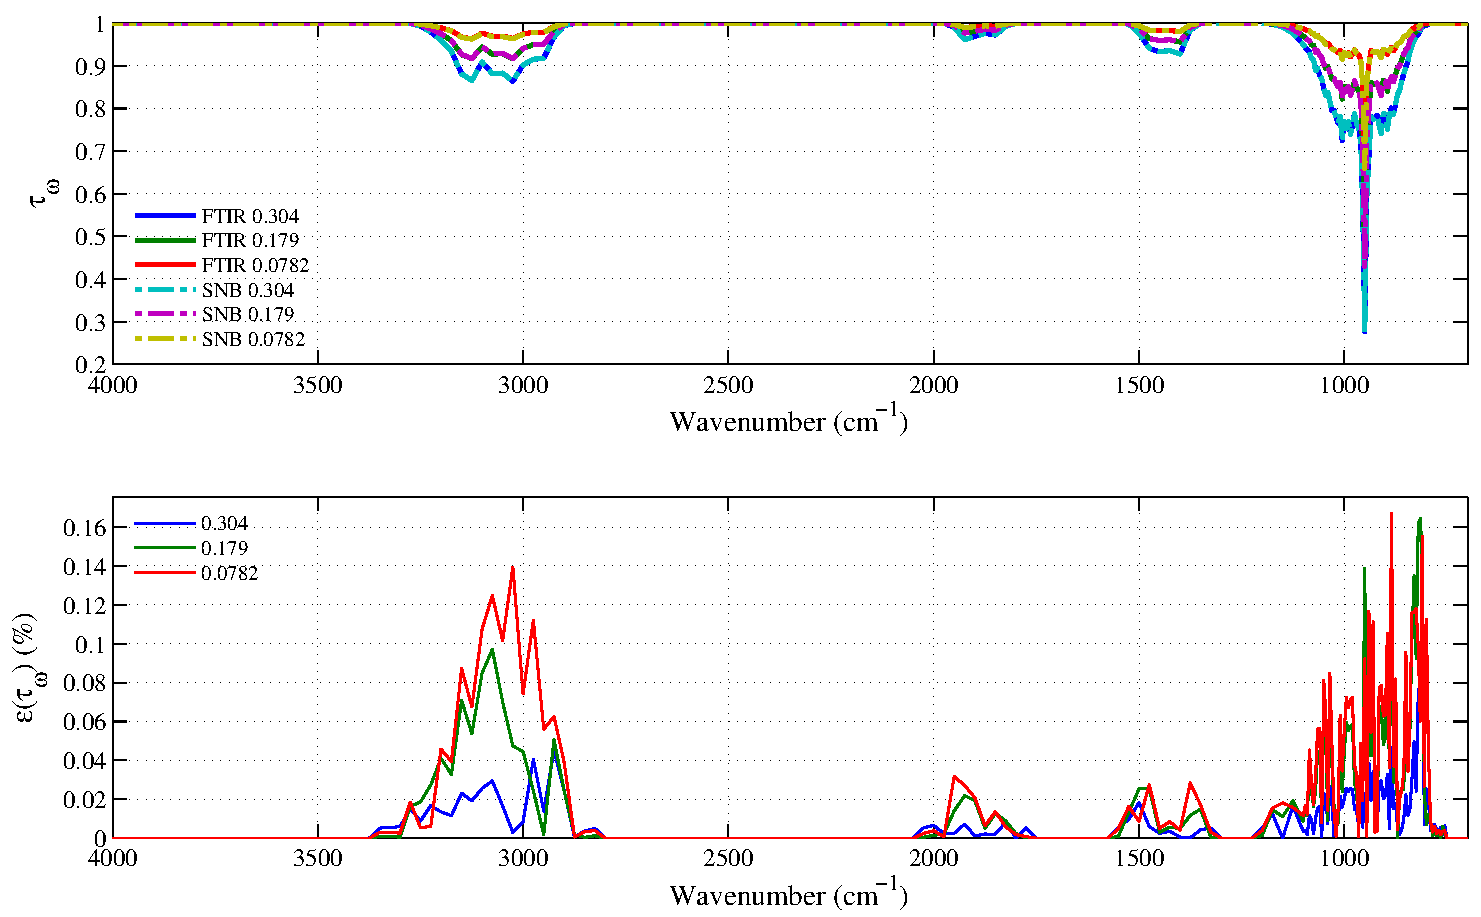
\includegraphics[width=\textwidth]{Figures/Comparison_Fit_Ethylene_MALKMUS_Temp500K.pdf}
\caption{Top: comparison between the experimental (FTIR, in solid lines) and the synthetic (dashed lines) spectral transmissivity profiles, denoted $\tau_{\omega}$, of an isothermal homogeneous column of ethylene. The synthetic profiles was generated using the Malkmus narrow band parameters presented in Figs.~\ref{fig:ethylene_kappa_beta1} to \ref{fig:ethylene_kappa_beta4}. Bottom: relative transmissivity error, denoted $\epsilon{(\tau_{\omega})}$, between the experiment and the synthetic profiles presented on the top figure. Three different pressure-paths are considered: 0.304, 0.179 and 0.0782 atm.cm. The gas temperature is set at 500~K and the total pressure is 101 kPa. Note: the experimental data resolution has been changed to match that of the narrow band model. \label{fig:ethylene_SNBVerify_500K}}
\end{figure}

\begin{figure}[p]
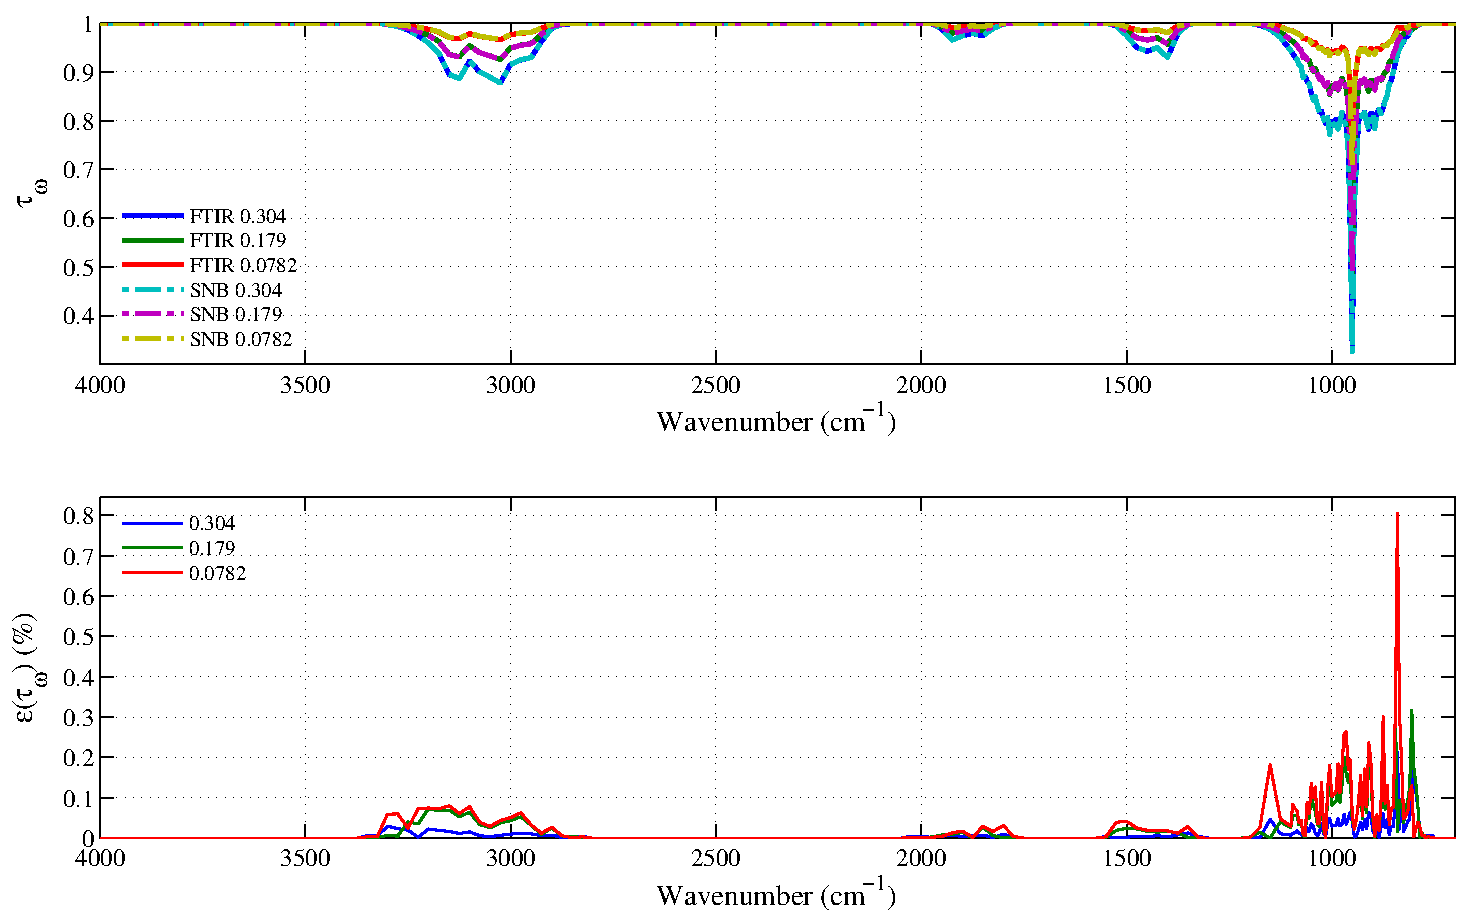
\includegraphics[width=\textwidth]{Figures/Comparison_Fit_Ethylene_MALKMUS_Temp601K.pdf}
\caption{Top: comparison between the experimental (FTIR, in solid lines) and the synthetic (dashed lines) spectral transmissivity profiles, denoted $\tau_{\omega}$, of an isothermal homogeneous column of ethylene. The synthetic profiles was generated using the Malkmus narrow band parameters presented in Figs.~\ref{fig:ethylene_kappa_beta1} to \ref{fig:ethylene_kappa_beta4}. Bottom: relative transmissivity error, denoted $\epsilon{(\tau_{\omega})}$, between the experiment and the synthetic profiles presented on the top figure. Three different pressure-paths are considered: 0.304, 0.179 and 0.0782 atm.cm. The gas temperature is set at 601~K and the total pressure is 101 kPa. Note: the experimental data resolution has been changed to match that of the narrow band model. \label{fig:ethylene_SNBVerify_601K}}
\end{figure}

\begin{figure}[p]
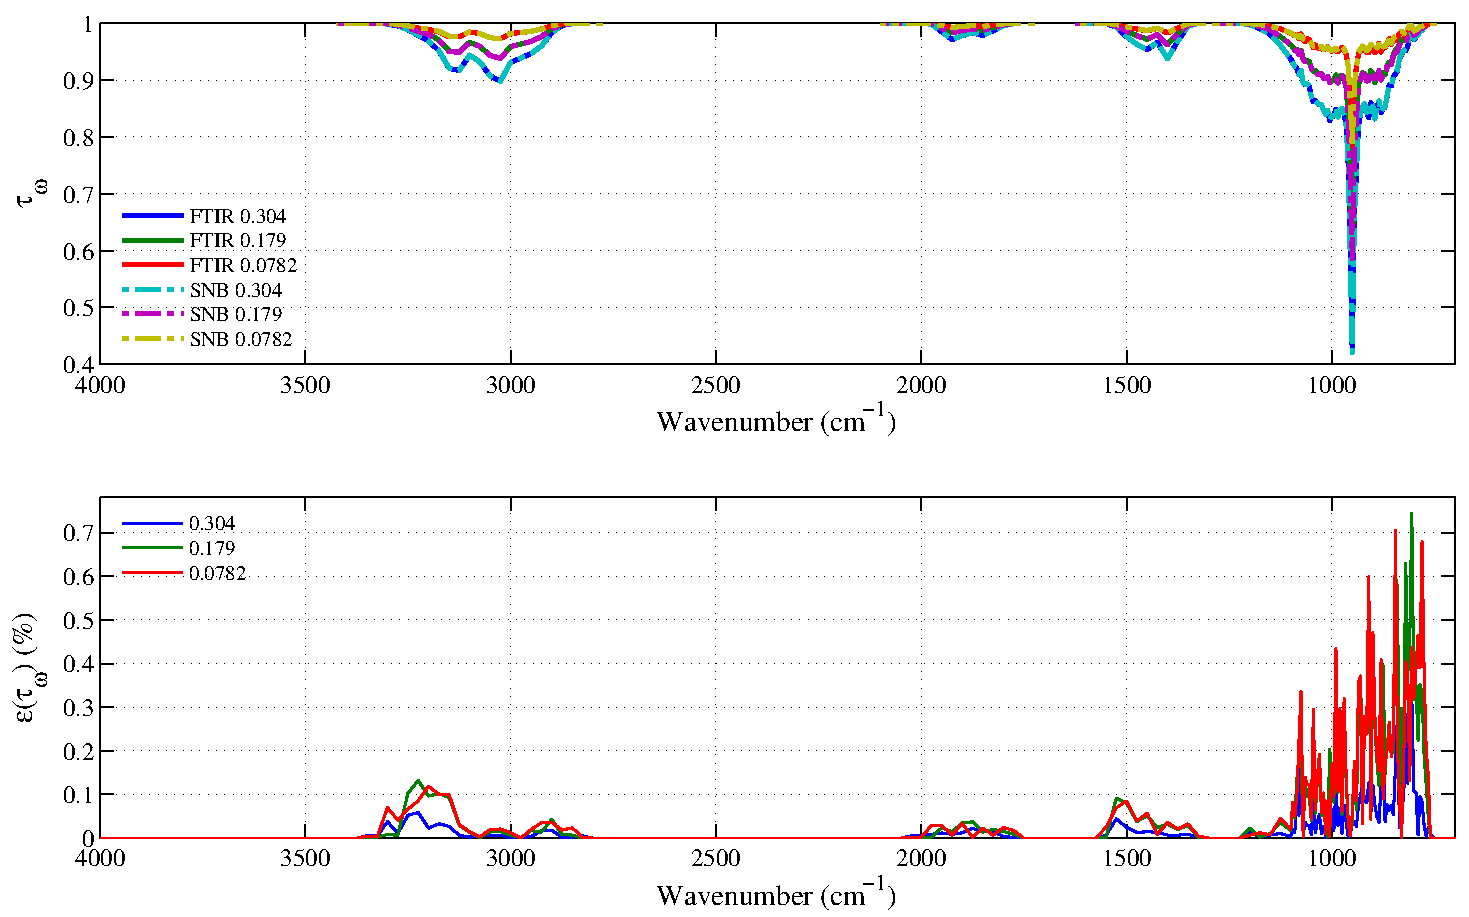
\includegraphics[width=\textwidth]{Figures/Comparison_Fit_Ethylene_MALKMUS_Temp801K.pdf}
\caption{Top: comparison between the experimental (FTIR, in solid lines) and the synthetic (dashed lines) spectral transmissivity profiles, denoted $\tau_{\omega}$, of an isothermal homogeneous column of ethylene. The synthetic profiles was generated using the Malkmus narrow band parameters presented in Figs.~\ref{fig:ethylene_kappa_beta1} to \ref{fig:ethylene_kappa_beta4}. Bottom: relative transmissivity error, denoted $\epsilon{(\tau_{\omega})}$, between the experiment and the synthetic profiles presented on the top figure. Three different pressure-paths are considered: 0.304, 0.179 and 0.0782 atm.cm. The gas temperature is set at 801~K and the total pressure is 101 kPa. Note: the experimental data resolution has been changed to match that of the narrow band model. \label{fig:ethylene_SNBVerify_801K}}
\end{figure}

\begin{figure}[p]
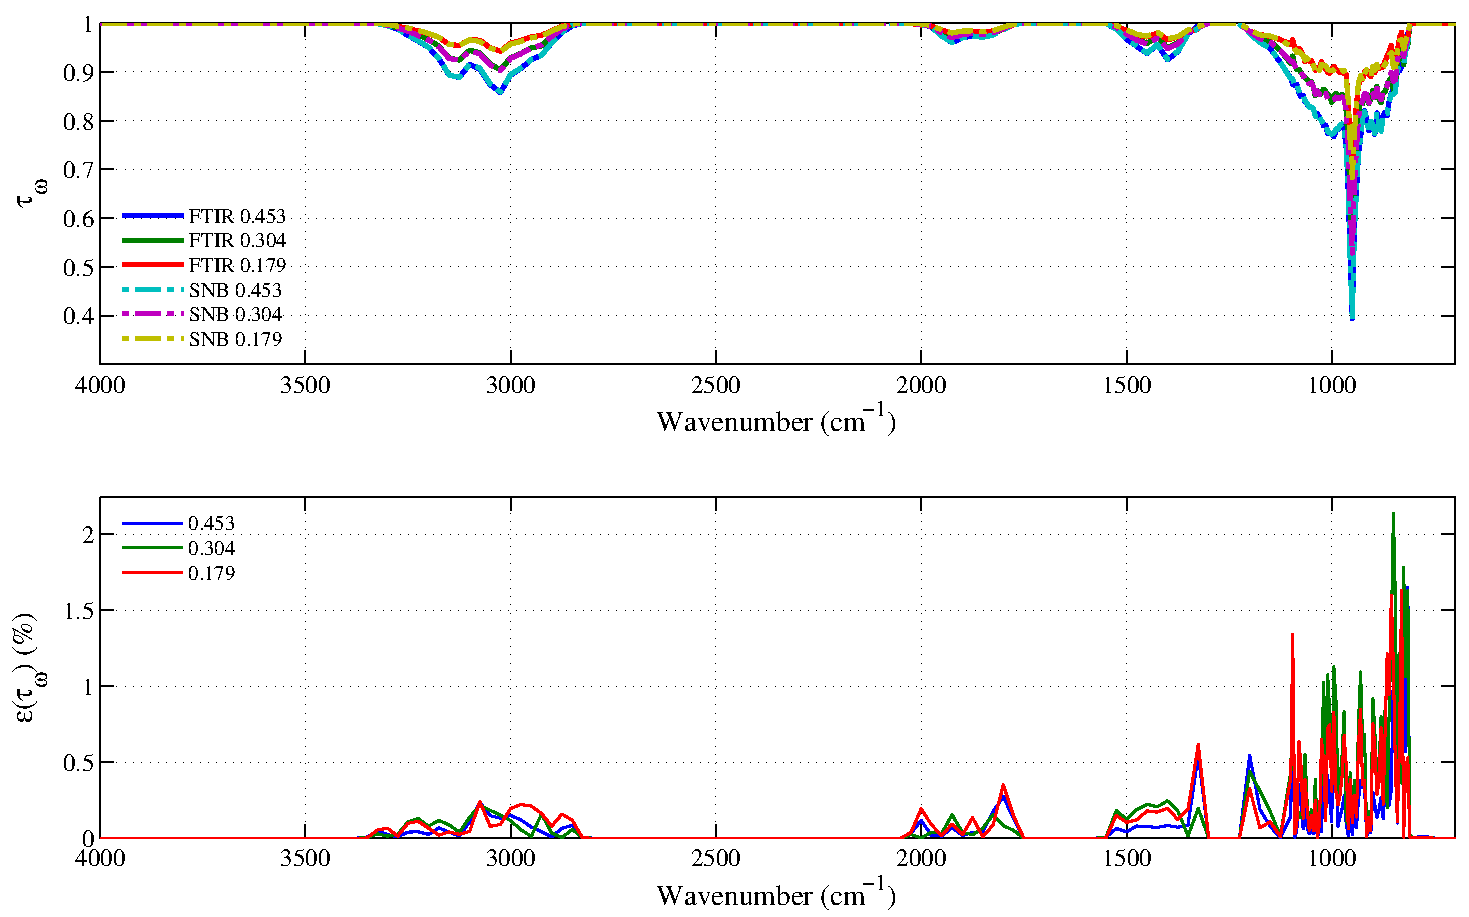
\includegraphics[width=\textwidth]{Figures/Comparison_Fit_Ethylene_MALKMUS_Temp1000K.pdf}
\caption{Top: comparison between the experimental (FTIR, in solid lines) and the synthetic (dashed lines) spectral transmissivity profiles, denoted $\tau_{\omega}$, of an isothermal homogeneous column of ethylene. The synthetic profiles was generated using the Malkmus narrow band parameters presented in Figs.~\ref{fig:ethylene_kappa_beta1} to \ref{fig:ethylene_kappa_beta4}. Bottom: relative transmissivity error, denoted $\epsilon{(\tau_{\omega})}$, between the experiment and the synthetic profiles presented on the top figure. Three different pressure-paths are considered: 0.304, 0.179 and 0.0782 atm.cm. The gas temperature is set at 1000~K and the total pressure is 101 kPa. Note: the experimental data resolution has been changed to match that of the narrow band model. \label{fig:ethylene_SNBVerify_1000K}}
\end{figure}


\clearpage

\section{Ethane: $\rm C_2H_6$}

\subsection{Integrated Band Intensity}

Ethane, $\rm C_2H_6$, has a three-fold axis of symmetry and belongs to the point group $D_{3d}$, \cite{Herzberg1949}. Being a non-linear molecule, it has 18 vibrational modes, but due to its symmetry, some modes are identical, and the number of distinct vibrational modes is reduced to 12. In RadCal, its spectra are defined by 3 distinct bands associated with different vibrational modes, see Table \ref{Table::C2H6}. The band from 730--1095~cm$^{-1}$ is associated with the rocking motion of the $\rm CH_3$ groups, the band from 1250--1700~cm$^{-1}$ is associated with the bending motion of the CH groups, and the main band between 2550--3375~cm$^{-1}$ is associated with the stretching of the CH groups.

The CH stretching band located from 2550--3375~cm$^{-1}$ has the lowest transmissivity, \textit{i.e.} highest absorption, and dominates absorption due to ethane for blackbody emissions at typical combustion temperatures between 1300~K and 1800~K, characteristic of sooting flames. At standard temperature and pressure, its integrated band intensity is more than 10 times the value of Band~2, and more than 20 times the value of Band~1.

\begin{table} [ht]
    \centering
    \caption{Spectral bands of $\rm C_2H_6$ included in RadCal.}
    \vspace{0.1in}
    \label{Table::C2H6}
    \begin{tabular}{|c|c|c|c|c|}
      \hline
      Band \# & \multicolumn{2}{|l|}{Bounds (cm$\rm ^{-1}$) } & Assignment & $\alpha(T=296 \; {\rm K}) \; (\rm {atm^{-1} cm^{-2}})$\\
      \cline{1-5}
      1 & 730  & 1095 &  $\rm CH_3$ Rock   &  30  \\
      2 & 1250 & 1700 &  $\rm CH$  Bend    &  64  \\
      3 & 2550 & 3375 &  $\rm CH$  Stretch &  774 \\
      \hline
    \end{tabular}
\end{table}

\subsection{Malkmus Narrow Band Parameters}

All the ethane IR spectral absorption data were obtained from high resolution FTIR experiments with temperatures varying from 296~K to 1000~K. The spectral absorption coefficients were obtained by fitting the experimental spectral transmissivity of a homogeneous column of isothermal ethane with a total pressure of 1~atm using the Malkmus model.

The ethane narrow band parameters, $\bar{\kappa}$ and $\beta$, for temperatures ranging from 296~K to 1000~K are plotted in Figures~\ref{fig:ethane_kappa_beta1}--\ref{fig:ethane_kappa_beta3} for Bands 1 to 3.

\newpage

\begin{figure}[p]
\begin{center}
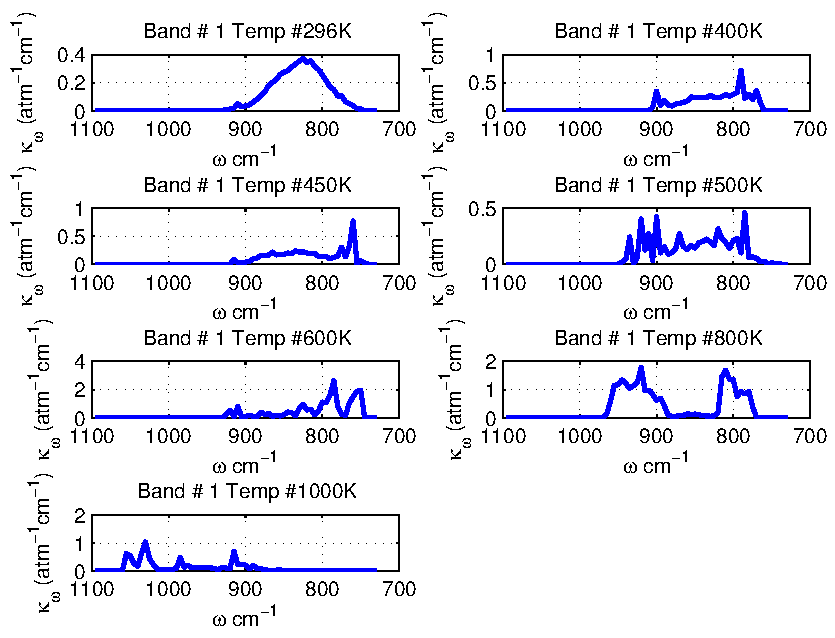
\includegraphics[width=5.0in]{Figures/Ethane_Kappa_Band1_MALKMUS.pdf}
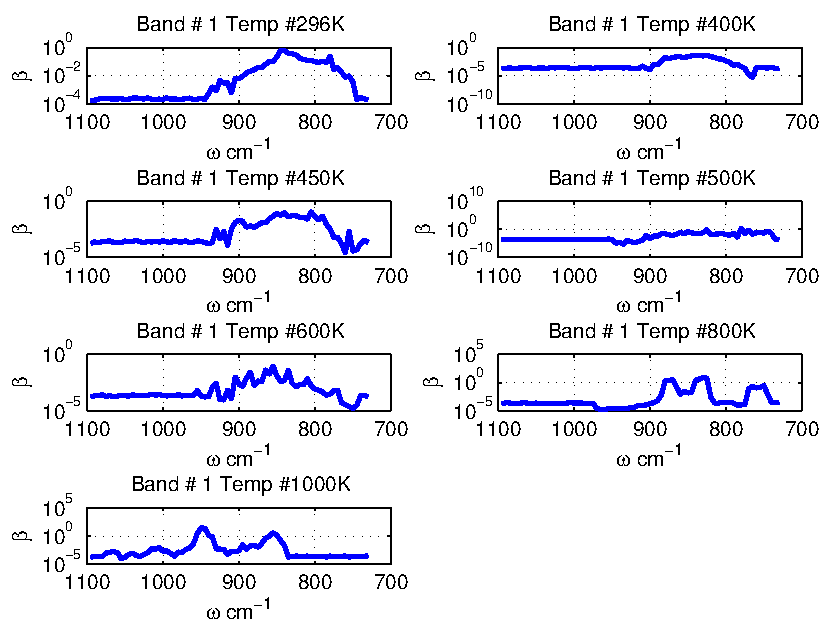
\includegraphics[width=5.0in]{Figures/Ethane_Beta_Band1_MALKMUS.pdf}
\end{center}
\caption{Ethane narrow band parameters $\bar{\kappa}$ and $\beta$ obtained for the 730--1095~cm$^{-1}$ band corresponding to the rocking motion of the $\rm CH_3$ chemical group. Temperatures plotted are: 296, 400, 450, 500, 600, 800, and 1000~K. The narrow band resolution $\Delta \om$ is 5~cm$^{-1}$.\label{fig:ethane_kappa_beta1}}
\end{figure}

\begin{figure}[p]
\begin{center}
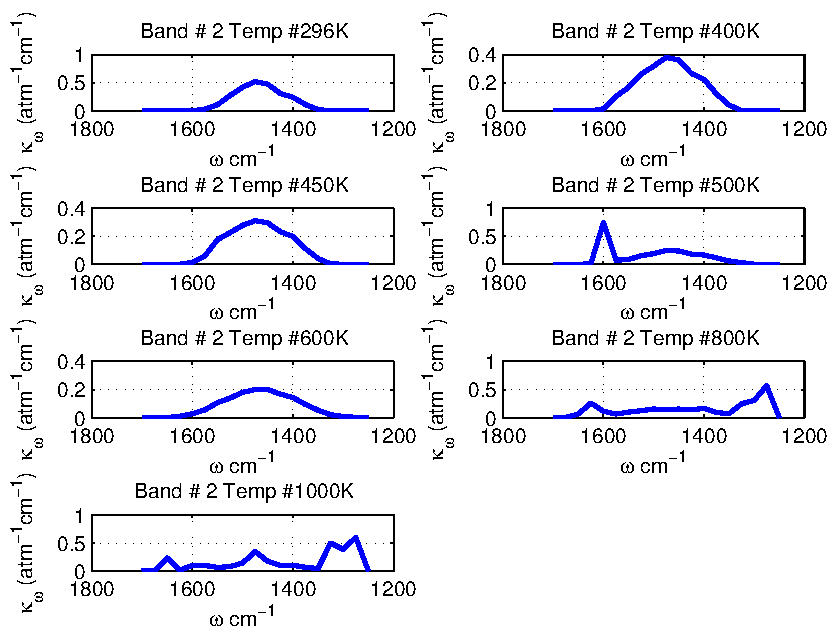
\includegraphics[width=5.0in]{Figures/Ethane_Kappa_Band2_MALKMUS.pdf}
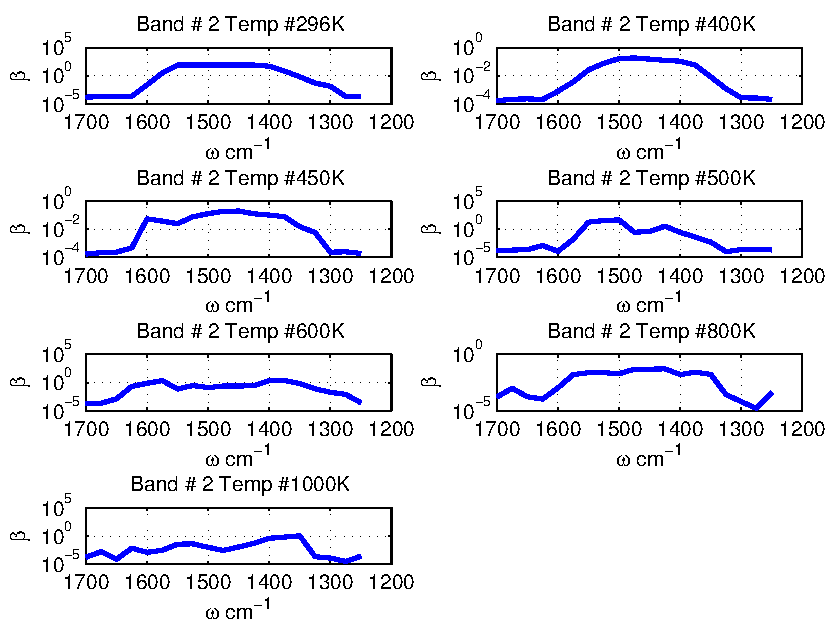
\includegraphics[width=5.0in]{Figures/Ethane_Beta_Band2_MALKMUS.pdf}
\end{center}
\caption{Ethane narrow band parameters $\bar{\kappa}$ and $\beta$ obtained for the 1250--1700~cm$^{-1}$ band corresponding to the bending motion of the $\rm CH$ chemical group. Temperatures plotted are: 296, 400, 450, 500, 600, 800, and 1000~K. The narrow band resolution $\Delta \om$ is 25~cm$^{-1}$.\label{fig:ethane_kappa_beta2}}
\end{figure}

\begin{figure}[p]
\begin{center}
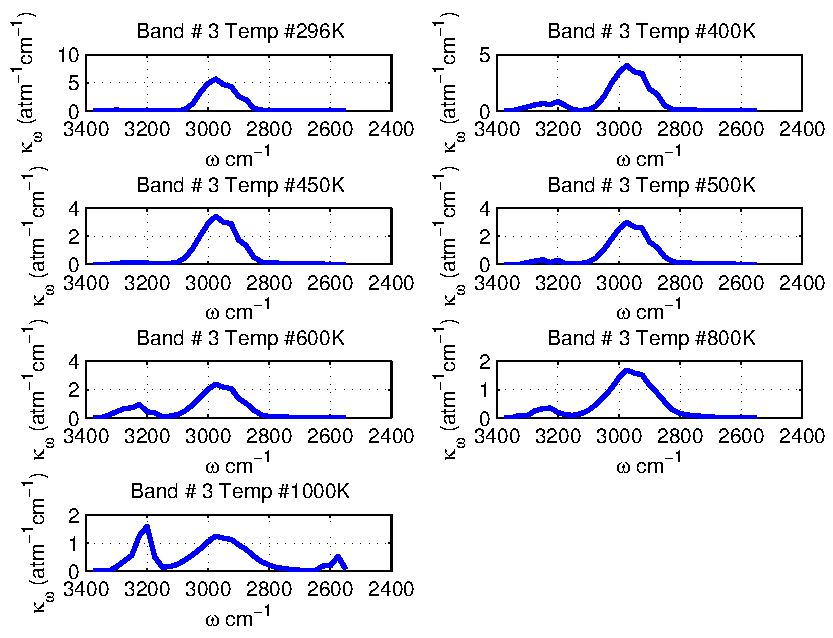
\includegraphics[width=5.0in]{Figures/Ethane_Kappa_Band3_MALKMUS.pdf}
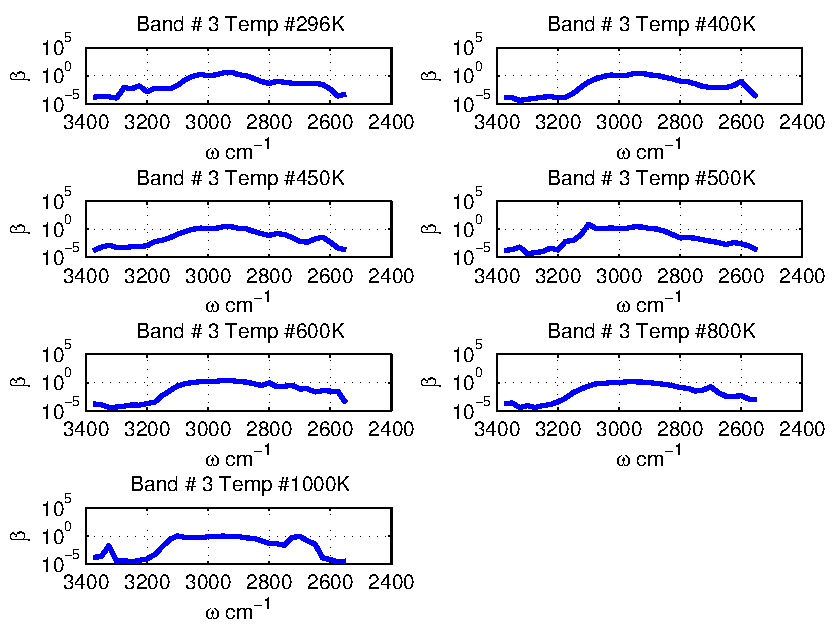
\includegraphics[width=5.0in]{Figures/Ethane_Beta_Band3_MALKMUS.pdf}
\end{center}
\caption{Ethane narrow band parameters $\bar{\kappa}$ and $\beta$ obtained for the 2550--3375~cm$^{-1}$ band corresponding to the stretching motion of the $\rm C-H$ chemical group. Temperatures plotted are: 296, 400, 450, 500, 600, 800, and 1000~K. The narrow band resolution $\Delta \om$ is 25~cm$^{-1}$.\label{fig:ethane_kappa_beta3}}
\end{figure}

\FloatBarrier

\subsection{Verification SNB Parameters}

To assess the accuracy of the narrow band parameters $\bar{\kappa}$ and $\beta$, synthetic transmissivities were constructed for the same experimental conditions as the FTIR data and compare with it. This subsection plots the comparison and the relative error in transmissivity (relative to FTIR measurements) using the ethane parameters presented in Figs.~\ref{fig:ethane_kappa_beta1} to \ref{fig:ethane_kappa_beta3}.

\begin{figure}[!h]
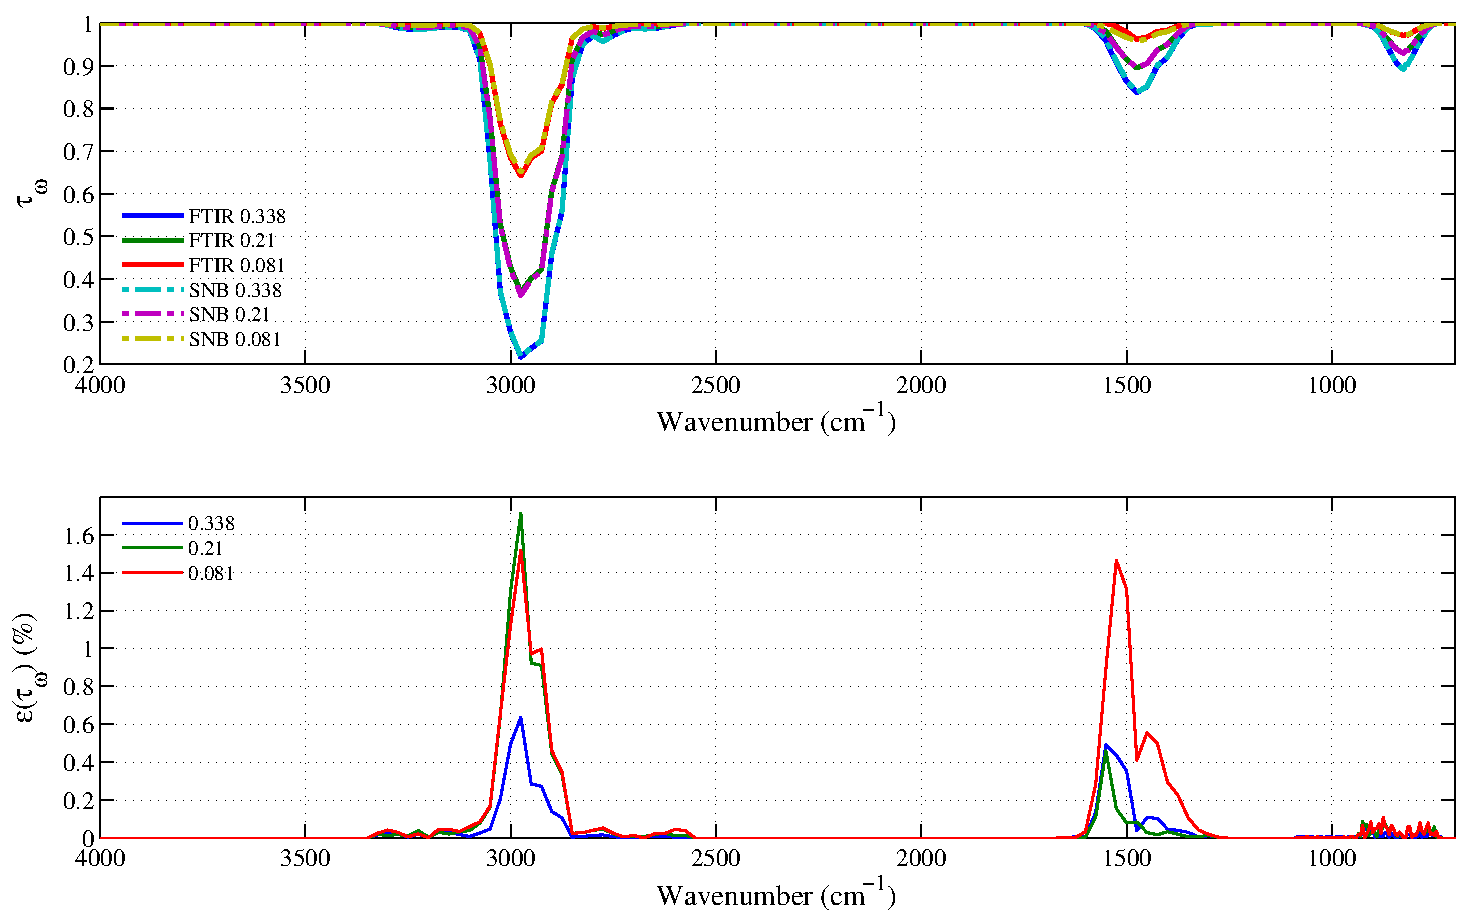
\includegraphics[width=\textwidth]{Figures/Comparison_Fit_Ethane_MALKMUS_Temp296K.pdf}
\caption{Top: comparison between the experimental (FTIR, in solid lines) and the synthetic (dashed lines) spectral transmissivity profiles, denoted $\tau_{\omega}$, of an isothermal homogeneous column of ethane. The synthetic profiles was generated using the Malkmus narrow band parameters presented in Figs.~\ref{fig:ethane_kappa_beta1} to \ref{fig:ethane_kappa_beta3}. Bottom: relative transmissivity error, denoted $\epsilon{(\tau_{\omega})}$, between the experiment and the synthetic profiles presented on the top figure. Three different pressure-paths are considered: 0.338, 0.21 and 0.081 atm.cm. The gas temperature is set at 296~K and the total pressure is 101 kPa. Note: the experimental data resolution has been changed to match that of the narrow band model. \label{fig:ethane_SNBVerify_296K}}
\end{figure}

\begin{figure}[p]
\includegraphics[width=\textwidth]{Figures/Comparison_Fit_Ethane_MALKMUS_Temp400K.pdf}
\caption{Top: comparison between the experimental (FTIR, in solid lines) and the synthetic (dashed lines) spectral transmissivity profiles, denoted $\tau_{\omega}$, of an isothermal homogeneous column of ethane. The synthetic profiles was generated using the Malkmus narrow band parameters presented in Figs.~\ref{fig:ethane_kappa_beta1} to \ref{fig:ethane_kappa_beta3}. Bottom: relative transmissivity error, denoted $\epsilon{(\tau_{\omega})}$, between the experiment and the synthetic profiles presented on the top figure. Three different pressure-paths are considered: 0.338, 0.21 and 0.081 atm.cm. The gas temperature is set at 400~K and the total pressure is 101 kPa. Note: the experimental data resolution has been changed to match that of the narrow band model. \label{fig:ethane_SNBVerify_400K}}
\end{figure}

\begin{figure}[p]
\includegraphics[width=\textwidth]{Figures/Comparison_Fit_Ethane_MALKMUS_Temp450K.pdf}
\caption{Top: comparison between the experimental (FTIR, in solid lines) and the synthetic (dashed lines) spectral transmissivity profiles, denoted $\tau_{\omega}$, of an isothermal homogeneous column of ethane. The synthetic profiles was generated using the Malkmus narrow band parameters presented in Figs.~\ref{fig:ethane_kappa_beta1} to \ref{fig:ethane_kappa_beta3}. Bottom: relative transmissivity error, denoted $\epsilon{(\tau_{\omega})}$, between the experiment and the synthetic profiles presented on the top figure. Three different pressure-paths are considered: 0.338, 0.21 and 0.081 atm.cm. The gas temperature is set at 450~K and the total pressure is 101 kPa. Note: the experimental data resolution has been changed to match that of the narrow band model. \label{fig:ethane_SNBVerify_450K}}
\end{figure}

\begin{figure}[p]
\includegraphics[width=\textwidth]{Figures/Comparison_Fit_Ethane_MALKMUS_Temp500K.pdf}
\caption{Top: comparison between the experimental (FTIR, in solid lines) and the synthetic (dashed lines) spectral transmissivity profiles, denoted $\tau_{\omega}$, of an isothermal homogeneous column of ethane. The synthetic profiles was generated using the Malkmus narrow band parameters presented in Figs.~\ref{fig:ethane_kappa_beta1} to \ref{fig:ethane_kappa_beta3}. Bottom: relative transmissivity error, denoted $\epsilon{(\tau_{\omega})}$, between the experiment and the synthetic profiles presented on the top figure. Three different pressure-paths are considered: 0.338, 0.21 and 0.081 atm.cm. The gas temperature is set at 500~K and the total pressure is 101 kPa. Note: the experimental data resolution has been changed to match that of the narrow band model. \label{fig:ethane_SNBVerify_500K}}
\end{figure}

\begin{figure}[p]
\includegraphics[width=\textwidth]{Figures/Comparison_Fit_Ethane_MALKMUS_Temp600K.pdf}
\caption{Top: comparison between the experimental (FTIR, in solid lines) and the synthetic (dashed lines) spectral transmissivity profiles, denoted $\tau_{\omega}$, of an isothermal homogeneous column of ethane. The synthetic profiles was generated using the Malkmus narrow band parameters presented in Figs.~\ref{fig:ethane_kappa_beta1} to \ref{fig:ethane_kappa_beta3}. Bottom: relative transmissivity error, denoted $\epsilon{(\tau_{\omega})}$, between the experiment and the synthetic profiles presented on the top figure. Three different pressure-paths are considered: 0.338, 0.21 and 0.081 atm.cm. The gas temperature is set at 600~K and the total pressure is 101 kPa. Note: the experimental data resolution has been changed to match that of the narrow band model. \label{fig:ethane_SNBVerify_600K}}
\end{figure}

\begin{figure}[p]
\includegraphics[width=\textwidth]{Figures/Comparison_Fit_Ethane_MALKMUS_Temp800K.pdf}
\caption{Top: comparison between the experimental (FTIR, in solid lines) and the synthetic (dashed lines) spectral transmissivity profiles, denoted $\tau_{\omega}$, of an isothermal homogeneous column of ethane. The synthetic profiles was generated using the Malkmus narrow band parameters presented in Figs.~\ref{fig:ethane_kappa_beta1} to \ref{fig:ethane_kappa_beta3}. Bottom: relative transmissivity error, denoted $\epsilon{(\tau_{\omega})}$, between the experiment and the synthetic profiles presented on the top figure. Three different pressure-paths are considered: 0.338, 0.21 and 0.081 atm.cm. The gas temperature is set at 800~K and the total pressure is 101 kPa. Note: the experimental data resolution has been changed to match that of the narrow band model. \label{fig:ethane_SNBVerify_800K}}
\end{figure}

\begin{figure}[p]
\includegraphics[width=\textwidth]{Figures/Comparison_Fit_Ethane_MALKMUS_Temp1000K.pdf}
\caption{Top: comparison between the experimental (FTIR, in solid lines) and the synthetic (dashed lines) spectral transmissivity profiles, denoted $\tau_{\omega}$, of an isothermal homogeneous column of ethane. The synthetic profiles was generated using the Malkmus narrow band parameters presented in Figs.~\ref{fig:ethane_kappa_beta1} to \ref{fig:ethane_kappa_beta3}. Bottom: relative transmissivity error, denoted $\epsilon{(\tau_{\omega})}$, between the experiment and the synthetic profiles presented on the top figure. Three different pressure-paths are considered: 0.338, 0.21 and 0.081 atm.cm. The gas temperature is set at 1000~K and the total pressure is 101 kPa. Note: the experimental data resolution has been changed to match that of the narrow band model. \label{fig:ethane_SNBVerify_1000K}}
\end{figure}


\clearpage

\section{Propylene: $\rm C_3H_6$}

\subsection{Integrated Band Intensity}

Propylene, $\rm C_3H_6$, has only one plane of symmetry and belongs to the point group $C_s$, \cite{Herzberg1949}. It has 21 vibrational modes. In RadCal, its spectrum is divided into three distinct bands, associated with different vibrational modes, see Table \ref{Table::C3H6}. The first band from 775--1150~cm$^{-1}$ is associated with the stretching motion of the carbon simple bond $\rm C-C$, the rocking motion of the $\rm CH_3$ group, and the out-of-plane bending motion of the $\rm = CH_2$ group. The second band from 1225--1975~cm$^{-1}$ is derived from the stretching motion of the carbon double bond $\rm C=C$ and the bending motion of the CH group. Finally, the third band from 2650--3275~cm$^{-1}$ is due to the stretching motion of the CH and $\rm = CH_2$ groups.

The strongest absorption bands for propylene are the 775--1150~cm$^{-1}$ (Band 1) and the 2650--3275~cm$^{-1}$ bands (Band 3). The 775--1150~cm$^{-1}$ band corresponds to radiation absorption and emission at near ambient temperature. The 2650--3275~cm$^{-1}$ band gives propylene strong absorption of radiation emitted by blackbody at high temperatures characteristic of sooting flames.

\begin{table}[ht]
   \centering
   \caption{Spectral bands of $\rm C_3H_6$ included in RadCal.}
   \vspace{0.1in}
   \label{Table::C3H6}
   \begin{tabular}{|c|c|c|c|c|}
    \hline
    Band \# & \multicolumn{2}{|l|}{Bounds (cm$\rm ^{-1}$) } & Assignment & $\alpha(T=296 \; {\rm K}) \; (\rm {atm^{-1} cm^{-2}})$\\
    \cline{1-5}
    1 & 775  & 1150 &  $\rm C-C$ Stretch, $\rm CH_3$ Rock & 296 \\
    2 & 1225 & 1975 &  $\rm C=C$ Stretch, $\rm CH$ Bend   & 271 \\
    3 & 2650 & 3275 &  $\rm CH$ \& $\rm CH_2$ Stretch      & 509 \\
    \hline
   \end{tabular}
\end{table}

\subsection{Malkmus Narrow Band Parameters}

All the propylene IR spectral absorption data were obtained from high resolution FTIR experiments with temperatures varying from 296~K to 1003~K. The spectral absorption coefficients were obtained by fitting the experimental spectral transmissivity of a homogeneous column of isothermal propylene with a total pressure of 1~atm using the Malkmus model.

The propylene narrow band parameters, $\bar{\kappa}$ and $\beta$, for temperatures ranging from 296~K to 1003~K are plotted in Figures~\ref{fig:propylene_kappa_beta1}--\ref{fig:propylene_kappa_beta3} for Bands 1 to 3.

\newpage

\begin{figure}[p]
\begin{center}
\includegraphics[width=5.0in]{Figures/Propylene_Kappa_Band1_MALKMUS.pdf}
\includegraphics[width=5.0in]{Figures/Propylene_Beta_Band1_MALKMUS.pdf}
\end{center}
\caption{Propylene narrow band parameters $\bar{\kappa}$ and $\beta$ obtained for the 775--1150~cm$^{-1}$ band corresponding to the rocking motion of the $\rm CH_3$ chemical group. Temperatures plotted are: 296, 390, 444, 491, 594, 793, and 1003~K. The narrow band resolution $\Delta \om$ is 5~cm$^{-1}$.\label{fig:propylene_kappa_beta1}}
\end{figure}

\begin{figure}[p]
\begin{center}
\includegraphics[width=5.0in]{Figures/Propylene_Kappa_Band2_MALKMUS.pdf}
\includegraphics[width=5.0in]{Figures/Propylene_Beta_Band2_MALKMUS.pdf}
\end{center}
\caption{Propylene narrow band parameters $\bar{\kappa}$ and $\beta$ obtained for the 1225--1975~cm$^{-1}$ band corresponding to the bending motion of the $\rm CH$ chemical group. Temperatures plotted are: 296, 390, 444, 491, 594, 793, and 1003~K. The narrow band resolution $\Delta \om$ is 25~cm$^{-1}$.\label{fig:propylene_kappa_beta2}}
\end{figure}

\begin{figure}[p]
\begin{center}
\includegraphics[width=5.0in]{Figures/Propylene_Kappa_Band3_MALKMUS.pdf}
\includegraphics[width=5.0in]{Figures/Propylene_Beta_Band3_MALKMUS.pdf}
\end{center}
\caption{Propylene narrow band parameters $\bar{\kappa}$ and $\beta$ obtained for the 2650--3275~cm$^{-1}$ band corresponding to the stretching motion of the $\rm C-H$ chemical group. Temperatures plotted are: 296, 390, 444, 491, 594, 793, and 1003~K. The narrow band resolution $\Delta \om$ is 25~cm$^{-1}$.\label{fig:propylene_kappa_beta3}}
\end{figure}

\FloatBarrier

\subsection{Verification SNB Parameters}

To assess the accuracy of the narrow band parameters $\bar{\kappa}$ and $\beta$, synthetic transmissivities were constructed for the same experimental conditions as the FTIR data and compare with it. This subsection plots the comparison and the relative error in transmissivity (relative to FTIR measurements) using the propylene parameters presented in Figs.~\ref{fig:propylene_kappa_beta1} to \ref{fig:propylene_kappa_beta3}.

\begin{figure}[!h]
\includegraphics[width=\textwidth]{Figures/Comparison_Fit_Propylene_MALKMUS_Temp296K.pdf}
\caption{Top: comparison between the experimental (FTIR, in solid lines) and the synthetic (dashed lines) spectral transmissivity profiles, denoted $\tau_{\omega}$, of an isothermal homogeneous column of propylene. The synthetic profiles was generated using the Malkmus narrow band parameters presented in Figs.~\ref{fig:propylene_kappa_beta1} to \ref{fig:propylene_kappa_beta3}. Bottom: relative transmissivity error, denoted $\epsilon{(\tau_{\omega})}$, between the experiment and the synthetic profiles presented on the top figure. Three different pressure-paths are considered: 0.475, 0.316 and 0.158 atm.cm. The gas temperature is set at 296~K and the total pressure is 101 kPa. Note: the experimental data resolution has been changed to match that of the narrow band model. \label{fig:propylene_SNBVerify_296K}}
\end{figure}

\begin{figure}[p]
\includegraphics[width=\textwidth]{Figures/Comparison_Fit_Propylene_MALKMUS_Temp390K.pdf}
\caption{Top: comparison between the experimental (FTIR, in solid lines) and the synthetic (dashed lines) spectral transmissivity profiles, denoted $\tau_{\omega}$, of an isothermal homogeneous column of propylene. The synthetic profiles was generated using the Malkmus narrow band parameters presented in Figs.~\ref{fig:propylene_kappa_beta1} to \ref{fig:propylene_kappa_beta3}. Bottom: relative transmissivity error, denoted $\epsilon{(\tau_{\omega})}$, between the experiment and the synthetic profiles presented on the top figure. Three different pressure-paths are considered: 0.475, 0.316 and 0.158 atm.cm. The gas temperature is set at 390~K and the total pressure is 101 kPa. Note: the experimental data resolution has been changed to match that of the narrow band model. \label{fig:propylene_SNBVerify_390K}}
\end{figure}

\begin{figure}[p]
\includegraphics[width=\textwidth]{Figures/Comparison_Fit_Propylene_MALKMUS_Temp444K.pdf}
\caption{Top: comparison between the experimental (FTIR, in solid lines) and the synthetic (dashed lines) spectral transmissivity profiles, denoted $\tau_{\omega}$, of an isothermal homogeneous column of propylene. The synthetic profiles was generated using the Malkmus narrow band parameters presented in Figs.~\ref{fig:propylene_kappa_beta1} to \ref{fig:propylene_kappa_beta3}. Bottom: relative transmissivity error, denoted $\epsilon{(\tau_{\omega})}$, between the experiment and the synthetic profiles presented on the top figure. Three different pressure-paths are considered: 0.475, 0.316 and 0.158 atm.cm. The gas temperature is set at 444~K and the total pressure is 101 kPa. Note: the experimental data resolution has been changed to match that of the narrow band model. \label{fig:propylene_SNBVerify_444K}}
\end{figure}

\begin{figure}[p]
\includegraphics[width=\textwidth]{Figures/Comparison_Fit_Propylene_MALKMUS_Temp491K.pdf}
\caption{Top: comparison between the experimental (FTIR, in solid lines) and the synthetic (dashed lines) spectral transmissivity profiles, denoted $\tau_{\omega}$, of an isothermal homogeneous column of propylene. The synthetic profiles was generated using the Malkmus narrow band parameters presented in Figs.~\ref{fig:propylene_kappa_beta1} to \ref{fig:propylene_kappa_beta3}. Bottom: relative transmissivity error, denoted $\epsilon{(\tau_{\omega})}$, between the experiment and the synthetic profiles presented on the top figure. Three different pressure-paths are considered: 0.475, 0.316 and 0.158 atm.cm. The gas temperature is set at 491~K and the total pressure is 101 kPa. Note: the experimental data resolution has been changed to match that of the narrow band model. \label{fig:propylene_SNBVerify_491K}}
\end{figure}

\begin{figure}[p]
\includegraphics[width=\textwidth]{Figures/Comparison_Fit_Propylene_MALKMUS_Temp594K.pdf}
\caption{Top: comparison between the experimental (FTIR, in solid lines) and the synthetic (dashed lines) spectral transmissivity profiles, denoted $\tau_{\omega}$, of an isothermal homogeneous column of propylene. The synthetic profiles was generated using the Malkmus narrow band parameters presented in Figs.~\ref{fig:propylene_kappa_beta1} to \ref{fig:propylene_kappa_beta3}. Bottom: relative transmissivity error, denoted $\epsilon{(\tau_{\omega})}$, between the experiment and the synthetic profiles presented on the top figure. Three different pressure-paths are considered: 0.475, 0.316 and 0.158 atm.cm. The gas temperature is set at 594~K and the total pressure is 101 kPa. Note: the experimental data resolution has been changed to match that of the narrow band model. \label{fig:propylene_SNBVerify_594K}}
\end{figure}

\begin{figure}[p]
\includegraphics[width=\textwidth]{Figures/Comparison_Fit_Propylene_MALKMUS_Temp793K.pdf}
\caption{Top: comparison between the experimental (FTIR, in solid lines) and the synthetic (dashed lines) spectral transmissivity profiles, denoted $\tau_{\omega}$, of an isothermal homogeneous column of propylene. The synthetic profiles was generated using the Malkmus narrow band parameters presented in Figs.~\ref{fig:propylene_kappa_beta1} to \ref{fig:propylene_kappa_beta3}. Bottom: relative transmissivity error, denoted $\epsilon{(\tau_{\omega})}$, between the experiment and the synthetic profiles presented on the top figure. Three different pressure-paths are considered: 0.475, 0.316 and 0.158 atm.cm. The gas temperature is set at 793~K and the total pressure is 101 kPa. Note: the experimental data resolution has been changed to match that of the narrow band model. \label{fig:propylene_SNBVerify_793K}}
\end{figure}

\begin{figure}[p]
\includegraphics[width=\textwidth]{Figures/Comparison_Fit_Propylene_MALKMUS_Temp1003K.pdf}
\caption{Top: comparison between the experimental (FTIR, in solid lines) and the synthetic (dashed lines) spectral transmissivity profiles, denoted $\tau_{\omega}$, of an isothermal homogeneous column of propylene. The synthetic profiles was generated using the Malkmus narrow band parameters presented in Figs.~\ref{fig:propylene_kappa_beta1} to \ref{fig:propylene_kappa_beta3}. Bottom: relative transmissivity error, denoted $\epsilon{(\tau_{\omega})}$, between the experiment and the synthetic profiles presented on the top figure. Three different pressure-paths are considered: 0.475, 0.316 and 0.158 atm.cm. The gas temperature is set at 1003~K and the total pressure is 101 kPa. Note: the experimental data resolution has been changed to match that of the narrow band model. \label{fig:propylene_SNBVerify_1003K}}
\end{figure}


\clearpage

\section{Propane: $\rm C_3H_8$}

\subsection{Integrated Band Intensity}

Propane, $\rm C_3H_8$, has two planes of symmetry and two axes of rotation and belongs to the point group $C_{2v}$ \cite{Herzberg1949}. It has 27 vibrational modes. In RadCal, its spectrum is divided into two distinct bands, associated with different vibrational modes, see Table \ref{Table::C3H8}. The propane IR spectrum is the result of the vibration-rotation modes of the $\rm C-C$, $\rm CH_2$, $\rm CH_3$ groups.
The first band from 1175--1675~cm$\rm ^{-1}$ is associated with the bending motion of the $\rm CH_3$ chemical group. The second band from 2550--3375~cm$\rm ^{-1}$ is associated with the stretching motion of the chemical groups $\rm CH_3$ and $\rm CH_2$. It is the strongest band; its integrated band intensity is about 10 times that of the 1175--1675~cm$\rm ^{-1}$ band.

\begin{table}[ht]
   \centering
   \caption{Spectral bands of $\rm C_3H_8$ included in RadCal.}
   \vspace{0.1in}
   \label{Table::C3H8}
   \begin{tabular}{|c|c|c|c|c|}
    \hline
    Band \# & \multicolumn{2}{|l|}{Bounds (cm$\rm ^{-1}$) } & Assignment & $\alpha(T=295 \; {\rm K}) \; (\rm {atm^{-1} cm^{-2}})$ \\
    \cline{1-5}
    1 & 1175 & 1675 &  $\rm CH_3$ Bending        & 122 \\
    2 & 2550 & 3375 &  $\rm CH_3, CH_2$ Stretch  & 1191 \\
    \hline
   \end{tabular}
\end{table}

\subsection{Malkmus Narrow Band Parameters}

All the propane IR spectral absorption data were obtained from high resolution FTIR experiments with temperatures varying from 295~K to 1009~K. The spectral absorption coefficients were obtained by fitting the experimental spectral transmissivity of a homogeneous column of isothermal propane with a total pressure of 1~atm using the Malkmus model.

The propane narrow band parameters, $\bar{\kappa}$ and $\beta$, for temperatures ranging from 295~K to 1009~K are plotted in Figures~\ref{fig:propane_kappa_beta1}--\ref{fig:propane_kappa_beta2} for Bands 1 to 2.

\newpage

\begin{figure}[p]
\begin{center}
\includegraphics[width=5.0in]{Figures/Propane_Kappa_Band1_MALKMUS.pdf}
\includegraphics[width=5.0in]{Figures/Propane_Beta_Band1_MALKMUS.pdf}
\end{center}
\caption{Propane narrow band parameters $\bar{\kappa}$ and $\beta$ obtained for the 1175--1675~cm$^{-1}$ band corresponding to the bending motion of the $\rm CH_3$ chemical group. Temperatures plotted are: 295, 396, 435, 513, 578, 790, and 1009~K. The narrow band resolution $\Delta \om$ is 5~cm$^{-1}$.\label{fig:propane_kappa_beta1}}
\end{figure}

\begin{figure}[p]
\begin{center}
\includegraphics[width=5.0in]{Figures/Propane_Kappa_Band2_MALKMUS.pdf}
\includegraphics[width=5.0in]{Figures/Propane_Beta_Band2_MALKMUS.pdf}
\end{center}
\caption{Propane narrow band parameters $\bar{\kappa}$ and $\beta$ obtained for the 2550--3375~cm$^{-1}$ band corresponding to the bending motion of the $\rm CH$ chemical group. Temperatures plotted are: 295, 396, 435, 513, 578, 790, and 1009~K. The narrow band resolution $\Delta \om$ is 25~cm$^{-1}$.\label{fig:propane_kappa_beta2}}
\end{figure}

\FloatBarrier

\subsection{Verification SNB Parameters}

To assess the accuracy of the narrow band parameters $\bar{\kappa}$ and $\beta$, synthetic transmissivities were constructed for the same experimental conditions as the FTIR data and compare with it. This subsection plots the comparison and the relative error in transmissivity (relative to FTIR measurements) using the propane parameters presented in Figs.~\ref{fig:propane_kappa_beta1} to \ref{fig:propane_kappa_beta2}.

\begin{figure}[!h]
\includegraphics[width=\textwidth]{Figures/Comparison_Fit_Propane_MALKMUS_Temp295K.pdf}
\caption{Top: comparison between the experimental (FTIR, in solid lines) and the synthetic (dashed lines) spectral transmissivity profiles, denoted $\tau_{\omega}$, of an isothermal homogeneous column of propane. The synthetic profiles was generated using the Malkmus narrow band parameters presented in Figs.~\ref{fig:propane_kappa_beta1} to \ref{fig:propane_kappa_beta2}. Bottom: relative transmissivity error, denoted $\epsilon{(\tau_{\omega})}$, between the experiment and the synthetic profiles presented on the top figure. Three different pressure-paths are considered: 0.127, 0.0791 and 0.0316 atm.cm. The gas temperature is set at 295~K and the total pressure is 101 kPa. Note: the experimental data resolution has been changed to match that of the narrow band model. \label{fig:propane_SNBVerify_295K}}
\end{figure}

\begin{figure}[p]
\includegraphics[width=\textwidth]{Figures/Comparison_Fit_Propane_MALKMUS_Temp396K.pdf}
\caption{Top: comparison between the experimental (FTIR, in solid lines) and the synthetic (dashed lines) spectral transmissivity profiles, denoted $\tau_{\omega}$, of an isothermal homogeneous column of propane. The synthetic profiles was generated using the Malkmus narrow band parameters presented in Figs.~\ref{fig:propane_kappa_beta1} to \ref{fig:propane_kappa_beta2}. Bottom: relative transmissivity error, denoted $\epsilon{(\tau_{\omega})}$, between the experiment and the synthetic profiles presented on the top figure. Three different pressure-paths are considered: 0.127, 0.0791 and 0.0316 atm.cm. The gas temperature is set at 396~K and the total pressure is 101 kPa. Note: the experimental data resolution has been changed to match that of the narrow band model. \label{fig:propane_SNBVerify_396K}}
\end{figure}

\begin{figure}[p]
\includegraphics[width=\textwidth]{Figures/Comparison_Fit_Propane_MALKMUS_Temp435K.pdf}
\caption{Top: comparison between the experimental (FTIR, in solid lines) and the synthetic (dashed lines) spectral transmissivity profiles, denoted $\tau_{\omega}$, of an isothermal homogeneous column of propane. The synthetic profiles was generated using the Malkmus narrow band parameters presented in Figs.~\ref{fig:propane_kappa_beta1} to \ref{fig:propane_kappa_beta2}. Bottom: relative transmissivity error, denoted $\epsilon{(\tau_{\omega})}$, between the experiment and the synthetic profiles presented on the top figure. Three different pressure-paths are considered: 0.127, 0.0791 and 0.0316 atm.cm. The gas temperature is set at 435~K and the total pressure is 101 kPa. Note: the experimental data resolution has been changed to match that of the narrow band model. \label{fig:propane_SNBVerify_435K}}
\end{figure}

\begin{figure}[p]
\includegraphics[width=\textwidth]{Figures/Comparison_Fit_Propane_MALKMUS_Temp513K.pdf}
\caption{Top: comparison between the experimental (FTIR, in solid lines) and the synthetic (dashed lines) spectral transmissivity profiles, denoted $\tau_{\omega}$, of an isothermal homogeneous column of propane. The synthetic profiles was generated using the Malkmus narrow band parameters presented in Figs.~\ref{fig:propane_kappa_beta1} to \ref{fig:propane_kappa_beta2}. Bottom: relative transmissivity error, denoted $\epsilon{(\tau_{\omega})}$, between the experiment and the synthetic profiles presented on the top figure. Three different pressure-paths are considered: 0.127, 0.0791 and 0.0316 atm.cm. The gas temperature is set at 513~K and the total pressure is 101 kPa. Note: the experimental data resolution has been changed to match that of the narrow band model. \label{fig:propane_SNBVerify_513K}}
\end{figure}

\begin{figure}[p]
\includegraphics[width=\textwidth]{Figures/Comparison_Fit_Propane_MALKMUS_Temp578K.pdf}
\caption{Top: comparison between the experimental (FTIR, in solid lines) and the synthetic (dashed lines) spectral transmissivity profiles, denoted $\tau_{\omega}$, of an isothermal homogeneous column of propane. The synthetic profiles was generated using the Malkmus narrow band parameters presented in Figs.~\ref{fig:propane_kappa_beta1} to \ref{fig:propane_kappa_beta2}. Bottom: relative transmissivity error, denoted $\epsilon{(\tau_{\omega})}$, between the experiment and the synthetic profiles presented on the top figure. Three different pressure-paths are considered: 0.127, 0.0791 and 0.0316 atm.cm. The gas temperature is set at 578~K and the total pressure is 101 kPa. Note: the experimental data resolution has been changed to match that of the narrow band model. \label{fig:propane_SNBVerify_578K}}
\end{figure}

\begin{figure}[p]
\includegraphics[width=\textwidth]{Figures/Comparison_Fit_Propane_MALKMUS_Temp790K.pdf}
\caption{Top: comparison between the experimental (FTIR, in solid lines) and the synthetic (dashed lines) spectral transmissivity profiles, denoted $\tau_{\omega}$, of an isothermal homogeneous column of propane. The synthetic profiles was generated using the Malkmus narrow band parameters presented in Figs.~\ref{fig:propane_kappa_beta1} to \ref{fig:propane_kappa_beta2}. Bottom: relative transmissivity error, denoted $\epsilon{(\tau_{\omega})}$, between the experiment and the synthetic profiles presented on the top figure. Three different pressure-paths are considered: 0.127, 0.0791 and 0.0316 atm.cm. The gas temperature is set at 790~K and the total pressure is 101 kPa. Note: the experimental data resolution has been changed to match that of the narrow band model. \label{fig:propane_SNBVerify_790K}}
\end{figure}

\begin{figure}[p]
\includegraphics[width=\textwidth]{Figures/Comparison_Fit_Propane_MALKMUS_Temp1009K.pdf}
\caption{Top: comparison between the experimental (FTIR, in solid lines) and the synthetic (dashed lines) spectral transmissivity profiles, denoted $\tau_{\omega}$, of an isothermal homogeneous column of propane. The synthetic profiles was generated using the Malkmus narrow band parameters presented in Figs.~\ref{fig:propane_kappa_beta1} to \ref{fig:propane_kappa_beta2}. Bottom: relative transmissivity error, denoted $\epsilon{(\tau_{\omega})}$, between the experiment and the synthetic profiles presented on the top figure. Three different pressure-paths are considered: 0.127, 0.0791 and 0.0316 atm.cm. The gas temperature is set at 1009~K and the total pressure is 101 kPa. Note: the experimental data resolution has been changed to match that of the narrow band model. \label{fig:propane_SNBVerify_1009K}}
\end{figure}


\clearpage

\section{Toluene: $\rm C_7H_8$}

\subsection{Integrated Band Intensity}

Toluene, $\rm C_7H_8$, has only one plane of symmetry; it belongs to the point group $C_{s}$~\cite{Herzberg1949}. Its IR spectrum is the result of the vibration-rotation modes of the $\rm C=C$, $\rm CH$, and $\rm CH_3$ groups. It has 39 vibrational modes. In RadCal, its IR spectrum has been divided into five distinct bands. The first band from 700--805~cm$\rm^{-1}$ is associated with the bending motion of the $\rm CH$ chemical group. The second band from 975--1175~cm$\rm^{-1}$ is associated with the bending motion of the $\rm CH$ chemical group. The third band from 1275--1650~cm$\rm^{-1}$ is associated with the bending motion of the $\rm CH_3$ chemical group. The fourth band from 1650--2075~cm$\rm^{-1}$ is associated with the stretching motion of the $\rm C=C$ chemical group. The fifth band from 2675--3225~cm$\rm^{-1}$ is associated with the stretching motion of the $\rm CH_3$ and $\rm CH$ chemical groups. The first and fifth bands have the highest integrated band intensity. See Table \ref{Table::C7H8}.
\begin{table}[ht]
   \centering
   \caption{Spectral bands of $\rm C_7H_8$ included in RadCal.}
   \vspace{0.1in}
   \label{Table::C7H8}
   \begin{tabular}{|c|c|c|c|c|}
    \hline
    Band \# & \multicolumn{2}{|l|}{Bounds (cm$\rm ^{-1}$) } & Assignment & $\alpha(T=300 \; {\rm K}) \; (\rm {atm^{-1} cm^{-2}})$\\
    \cline{1-5}
    1 & 700  & 805  &  $\rm CH$ Bending      & 234 \\
    2 & 975  & 1175 &  $\rm CH$ Bending      & 40  \\
    3 & 1275 & 1650 &  $\rm CH_3$ Bending    & 166 \\
    4 & 1650 & 2075 &  $\rm C=C$ Stretching  & 205 \\
    5 & 2675 & 3225 &  $\rm CH_3$, $\rm CH$  Stretching & 507  \\
    \hline
   \end{tabular}
\end{table}

\subsection{Malkmus Narrow Band Parameters}

All the toluene IR spectral absorption data were obtained from high resolution FTIR experiments with temperatures varying from 300~K to 999~K. The spectral absorption coefficients were obtained by fitting the experimental spectral transmissivity of a homogeneous column of isothermal toluene with a total pressure of 1~atm using the Malkmus model.

The toluene narrow band parameters, $\bar{\kappa}$ and $\beta$, for temperatures ranging from 300~K to 999~K are plotted in Figures~\ref{fig:toluene_kappa_beta1}--\ref{fig:toluene_kappa_beta5} for Bands 1 to 5.

\newpage

\begin{figure}[p]
\begin{center}
\includegraphics[width=5.0in]{Figures/Toluene_Kappa_Band1_MALKMUS.pdf}
\includegraphics[width=5.0in]{Figures/Toluene_Beta_Band1_MALKMUS.pdf}
\end{center}
\caption{Toluene narrow band parameters $\bar{\kappa}$ and $\beta$ obtained for the 700--805~cm$^{-1}$ band corresponding to the bending motion of the $\rm CH$ chemical group. Temperatures plotted are: 300, 396, 440, 477, 587, 795, and 999~K. The narrow band resolution $\Delta \om$ is 5~cm$^{-1}$.\label{fig:toluene_kappa_beta1}}
\end{figure}

\begin{figure}[p]
\begin{center}
\includegraphics[width=5.0in]{Figures/Toluene_Kappa_Band2_MALKMUS.pdf}
\includegraphics[width=5.0in]{Figures/Toluene_Beta_Band2_MALKMUS.pdf}
\end{center}
\caption{Toluene narrow band parameters $\bar{\kappa}$ and $\beta$ obtained for the 975--1175~cm$^{-1}$ band corresponding to the bending motion of the $\rm CH$ chemical group. Temperatures plotted are: 300, 396, 440, 477, 587, 795, and 999~K. The narrow band resolution $\Delta \om$ is 5~cm$^{-1}$.\label{fig:toluene_kappa_beta2}}
\end{figure}

\begin{figure}[p]
\begin{center}
\includegraphics[width=5.0in]{Figures/Toluene_Kappa_Band3_MALKMUS.pdf}
\includegraphics[width=5.0in]{Figures/Toluene_Beta_Band3_MALKMUS.pdf}
\end{center}
\caption{Toluene narrow band parameters $\bar{\kappa}$ and $\beta$ obtained for the 1275--1650~cm$^{-1}$ band corresponding to the bending motion of the $\rm CH_3$ chemical group. Temperatures plotted are: 300, 396, 440, 477, 587, 795, and 999~K. The narrow band resolution $\Delta \om$ is 25~cm$^{-1}$.\label{fig:toluene_kappa_beta3}}
\end{figure}

\begin{figure}[p]
\begin{center}
\includegraphics[width=5.0in]{Figures/Toluene_Kappa_Band4_MALKMUS.pdf}
\includegraphics[width=5.0in]{Figures/Toluene_Beta_Band4_MALKMUS.pdf}
\end{center}
\caption{Toluene narrow band parameters $\bar{\kappa}$ and $\beta$ obtained for the 1650--2075~cm$^{-1}$ band corresponding to the stretching motion of the $\rm C=C$ chemical group. Temperatures plotted are: 300, 396, 440, 477, 587, 795, and 999~K. The narrow band resolution $\Delta \om$ is 25~cm$^{-1}$.\label{fig:toluene_kappa_beta4}}
\end{figure}

\begin{figure}[p]
\begin{center}
\includegraphics[width=5.0in]{Figures/Toluene_Kappa_Band5_MALKMUS.pdf}
\includegraphics[width=5.0in]{Figures/Toluene_Beta_Band5_MALKMUS.pdf}
\end{center}
\caption{Toluene narrow band parameters $\bar{\kappa}$ and $\beta$ obtained for the 2675--3225~cm$^{-1}$ band corresponding to the bending motion of the $\rm CH_3$ and $\rm CH$ chemical groups. Temperatures plotted are: 300, 396, 440, 477, 587, 795, and 999~K. The narrow band resolution $\Delta \om$ is 25~cm$^{-1}$.\label{fig:toluene_kappa_beta5}}
\end{figure}

\FloatBarrier

\subsection{Verification SNB Parameters}

To assess the accuracy of the narrow band parameters $\bar{\kappa}$ and $\beta$, synthetic transmissivities were constructed for the same experimental conditions as the FTIR data and compare with it. This subsection plots the comparison and the relative error in transmissivity (relative to FTIR measurements) using the toluene parameters presented in Figs.~\ref{fig:toluene_kappa_beta1} to \ref{fig:toluene_kappa_beta5}.

\begin{figure}[!h]
\includegraphics[width=\textwidth]{Figures/Comparison_Fit_Toluene_MALKMUS_Temp300K.pdf}
\caption{Top: comparison between the experimental (FTIR, in solid lines) and the synthetic (dashed lines) spectral transmissivity profiles, denoted $\tau_{\omega}$, of an isothermal homogeneous column of toluene. The synthetic profiles was generated using the Malkmus narrow band parameters presented in Figs.~\ref{fig:toluene_kappa_beta1} to \ref{fig:toluene_kappa_beta5}. Bottom: relative transmissivity error, denoted $\epsilon{(\tau_{\omega})}$, between the experiment and the synthetic profiles presented on the top figure. Three different pressure-paths are considered: 0.135, 0.101 and 0.0806 atm.cm. The gas temperature is set at 300~K and the total pressure is 101 kPa. Note: the experimental data resolution has been changed to match that of the narrow band model. \label{fig:toluene_SNBVerify_300K}}
\end{figure}

\begin{figure}[p]
\includegraphics[width=\textwidth]{Figures/Comparison_Fit_Toluene_MALKMUS_Temp396K.pdf}
\caption{Top: comparison between the experimental (FTIR, in solid lines) and the synthetic (dashed lines) spectral transmissivity profiles, denoted $\tau_{\omega}$, of an isothermal homogeneous column of toluene. The synthetic profiles was generated using the Malkmus narrow band parameters presented in Figs.~\ref{fig:toluene_kappa_beta1} to \ref{fig:toluene_kappa_beta5}. Bottom: relative transmissivity error, denoted $\epsilon{(\tau_{\omega})}$, between the experiment and the synthetic profiles presented on the top figure. Three different pressure-paths are considered: 0.124, 0.0956 and 0.0808 atm.cm. The gas temperature is set at 396~K and the total pressure is 101 kPa. Note: the experimental data resolution has been changed to match that of the narrow band model. \label{fig:toluene_SNBVerify_396K}}
\end{figure}

\begin{figure}[p]
\includegraphics[width=\textwidth]{Figures/Comparison_Fit_Toluene_MALKMUS_Temp440K.pdf}
\caption{Top: comparison between the experimental (FTIR, in solid lines) and the synthetic (dashed lines) spectral transmissivity profiles, denoted $\tau_{\omega}$, of an isothermal homogeneous column of toluene. The synthetic profiles was generated using the Malkmus narrow band parameters presented in Figs.~\ref{fig:toluene_kappa_beta1} to \ref{fig:toluene_kappa_beta5}. Bottom: relative transmissivity error, denoted $\epsilon{(\tau_{\omega})}$, between the experiment and the synthetic profiles presented on the top figure. Three different pressure-paths are considered:0.109, 0.0844 and 0.0741. The gas temperature is set at 440~K and the total pressure is 101 kPa. Note: the experimental data resolution has been changed to match that of the narrow band model. \label{fig:toluene_SNBVerify_440K}}
\end{figure}

\begin{figure}[p]
\includegraphics[width=\textwidth]{Figures/Comparison_Fit_Toluene_MALKMUS_Temp477K.pdf}
\caption{Top: comparison between the experimental (FTIR, in solid lines) and the synthetic (dashed lines) spectral transmissivity profiles, denoted $\tau_{\omega}$, of an isothermal homogeneous column of toluene. The synthetic profiles was generated using the Malkmus narrow band parameters presented in Figs.~\ref{fig:toluene_kappa_beta1} to \ref{fig:toluene_kappa_beta5}. Bottom: relative transmissivity error, denoted $\epsilon{(\tau_{\omega})}$, between the experiment and the synthetic profiles presented on the top figure. Three different pressure-paths are considered: 0.125, 0.096 and 0.0828 atm.cm. The gas temperature is set at 477~K and the total pressure is 101 kPa. Note: the experimental data resolution has been changed to match that of the narrow band model. \label{fig:toluene_SNBVerify_477K}}
\end{figure}

\begin{figure}[p]
\includegraphics[width=\textwidth]{Figures/Comparison_Fit_Toluene_MALKMUS_Temp587K.pdf}
\caption{Top: comparison between the experimental (FTIR, in solid lines) and the synthetic (dashed lines) spectral transmissivity profiles, denoted $\tau_{\omega}$, of an isothermal homogeneous column of toluene. The synthetic profiles was generated using the Malkmus narrow band parameters presented in Figs.~\ref{fig:toluene_kappa_beta1} to \ref{fig:toluene_kappa_beta5}. Bottom: relative transmissivity error, denoted $\epsilon{(\tau_{\omega})}$, between the experiment and the synthetic profiles presented on the top figure. Three different pressure-paths are considered: 0.118, 0.0958 and 0.0809 atm.cm. The gas temperature is set at 587~K and the total pressure is 101 kPa. Note: the experimental data resolution has been changed to match that of the narrow band model. \label{fig:toluene_SNBVerify_587K}}
\end{figure}

\begin{figure}[p]
\includegraphics[width=\textwidth]{Figures/Comparison_Fit_Toluene_MALKMUS_Temp795K.pdf}
\caption{Top: comparison between the experimental (FTIR, in solid lines) and the synthetic (dashed lines) spectral transmissivity profiles, denoted $\tau_{\omega}$, of an isothermal homogeneous column of toluene. The synthetic profiles was generated using the Malkmus narrow band parameters presented in Figs.~\ref{fig:toluene_kappa_beta1} to \ref{fig:toluene_kappa_beta5}. Bottom: relative transmissivity error, denoted $\epsilon{(\tau_{\omega})}$, between the experiment and the synthetic profiles presented on the top figure. Three different pressure-paths are considered: 0.127, 0.0963 and 0.0831 atm.cm. The gas temperature is set at 795~K and the total pressure is 101 kPa. Note: the experimental data resolution has been changed to match that of the narrow band model. \label{fig:toluene_SNBVerify_795K}}
\end{figure}


\begin{figure}[p]
\includegraphics[width=\textwidth]{Figures/Comparison_Fit_Toluene_MALKMUS_Temp999K.pdf}
\caption{Top: comparison between the experimental (FTIR, in solid lines) and the synthetic (dashed lines) spectral transmissivity profiles, denoted $\tau_{\omega}$, of an isothermal homogeneous column of toluene. The synthetic profiles was generated using the Malkmus narrow band parameters presented in Figs.~\ref{fig:toluene_kappa_beta1} to \ref{fig:toluene_kappa_beta5}. Bottom: relative transmissivity error, denoted $\epsilon{(\tau_{\omega})}$, between the experiment and the synthetic profiles presented on the top figure. Three different pressure-paths are considered: 0.138, 0.103 and 0.0893 atm.cm. The gas temperature is set at 999~K and the total pressure is 101 kPa. Note: the experimental data resolution has been changed to match that of the narrow band model. \label{fig:toluene_SNBVerify_999K}}
\end{figure}


\clearpage

\section{\textit{n}-Heptane: $\rm C_7H_{16}$}

\subsection{Integrated Band Intensity}

\textit{n}-heptane, $\rm C_7H_16$, has two planes of symmetry and two axes of rotation. It belongs to the point group $C_{2v}$~\cite{Herzberg1949}. The \textit{n}-heptane IR spectrum results from the vibration-rotation modes of the $\rm C-C$, $\rm CH_2$, and $\rm CH_3$ groups. It has 63 vibrational modes. In RadCal, its IR spectrum has been divided into two distinct bands. The first band from 1100--1800~cm$\rm^{-1}$ is associated with the bending motion of the $\rm CH_2$ and $\rm CH_3$ chemical groups. The second band from 2250--3275~cm$\rm^{-1}$ is associated with the stretching motion of the $\rm CH_2$ and $\rm CH_3$ chemical groups. This band has the highest integrated band intensity. Its value is more than 10 times that of the first band, see Table \ref{Table::C7H16}.
\begin{table}[ht]
   \centering
   \caption{Spectral bands of $\rm C_7H_{16}$ included in RadCal.}
   \vspace{0.1in}
   \label{Table::C7H16}
   \begin{tabular}{|c|c|c|c|c|}
    \hline
    Band \# & \multicolumn{2}{|l|}{Bounds (cm$\rm ^{-1}$) } & Assignment & $\alpha(T=293 \; {\rm K}) \; (\rm {atm^{-1} cm^{-2}})$\\
    \cline{1-5}
    1 & 1100  & 1800 &  $\rm CH_2, CH_3$ Bending    & 304 \\
    2 & 2250  & 3275 &  $\rm CH_2, CH_3$ Stretching & 3165 \\
    \hline
   \end{tabular}
\end{table}

\subsection{Malkmus Narrow Band Parameters}

All the \textit{n}-heptane IR spectral absorption data were obtained from high resolution FTIR experiments with temperatures varying from 293~K to 794~K. The spectral absorption coefficients were obtained by fitting the experimental spectral transmissivity of a homogeneous column of isothermal \textit{n}-heptane with a total pressure of 1~atm using the Malkmus model.

The \textit{n}-heptane narrow band parameters, $\bar{\kappa}$ and $\beta$, for temperatures ranging from 293~K to 1000~K are plotted in Figures~\ref{fig:nheptane_kappa_beta1}--\ref{fig:nheptane_kappa_beta2} for Bands 1 and 2.

\newpage

\begin{figure}[p]
\begin{center}
\includegraphics[width=5.0in]{Figures/Heptane_Kappa_Band1_MALKMUS.pdf}
\includegraphics[width=5.0in]{Figures/Heptane_Beta_Band1_MALKMUS.pdf}
\end{center}
\caption{\textit{n}-heptane narrow band parameters $\bar{\kappa}$ and $\beta$ obtained for the 1100--1800~cm$^{-1}$ band corresponding to the bending motion of the $\rm CH_2$ and $\rm CH_3$ chemical groups. Temperatures plotted are: 293, 400, 450, 490, 593, 794, and 1000~K. The narrow band resolution $\Delta \om$ is 25~cm$^{-1}$.\label{fig:nheptane_kappa_beta1}}
\end{figure}

\begin{figure}[p]
\begin{center}
\includegraphics[width=5.0in]{Figures/Heptane_Kappa_Band2_MALKMUS.pdf}
\includegraphics[width=5.0in]{Figures/Heptane_Beta_Band2_MALKMUS.pdf}
\end{center}
\caption{\textit{n}-heptane narrow band parameters $\bar{\kappa}$ and $\beta$ obtained for the 2250--3275~cm$^{-1}$ band corresponding to the stretching motion of the $\rm CH_2$ and $\rm CH_3$ chemical groups. Temperatures plotted are: 293, 400, 450, 490, 593, 794, and 1000~K. The narrow band resolution $\Delta \om$ is 25~cm$^{-1}$.\label{fig:nheptane_kappa_beta2}}
\end{figure}

\FloatBarrier

\subsection{Verification SNB Parameters}

To assess the accuracy of the narrow band parameters $\bar{\kappa}$ and $\beta$, synthetic transmissivities were constructed for the same experimental conditions as the FTIR data and compare with it. This subsection plots the comparison and the relative error in transmissivity (relative to FTIR measurements) using the \textit{n}-heptane parameters presented in Figs.~\ref{fig:nheptane_kappa_beta1} to \ref{fig:nheptane_kappa_beta2}.

\begin{figure}[!h]
\includegraphics[width=\textwidth]{Figures/Comparison_Fit_Heptane_MALKMUS_Temp293K.pdf}
\caption{Top: comparison between the experimental (FTIR, in solid lines) and the synthetic (dashed lines) spectral transmissivity profiles, denoted $\tau_{\omega}$, of an isothermal homogeneous column of \textit{n}-heptane. The synthetic profiles was generated using the Malkmus narrow band parameters presented in Figs.~\ref{fig:nheptane_kappa_beta1} to \ref{fig:nheptane_kappa_beta2}. Bottom: relative transmissivity error, denoted $\epsilon{(\tau_{\omega})}$, between the experiment and the synthetic profiles presented on the top figure. Three different pressure-paths are considered: 0.0492, 0.0312 and 0.015 atm.cm. The gas temperature is set at 293~K and the total pressure is 101 kPa. Note: the experimental data resolution has been changed to match that of the narrow band model. \label{fig:nheptane_SNBVerify_293K}}
\end{figure}

\begin{figure}[p]
\includegraphics[width=\textwidth]{Figures/Comparison_Fit_Heptane_MALKMUS_Temp400K.pdf}
\caption{Top: comparison between the experimental (FTIR, in solid lines) and the synthetic (dashed lines) spectral transmissivity profiles, denoted $\tau_{\omega}$, of an isothermal homogeneous column of \textit{n}-heptane. The synthetic profiles was generated using the Malkmus narrow band parameters presented in Figs.~\ref{fig:nheptane_kappa_beta1} to \ref{fig:nheptane_kappa_beta2}. Bottom: relative transmissivity error, denoted $\epsilon{(\tau_{\omega})}$, between the experiment and the synthetic profiles presented on the top figure. Three different pressure-paths are considered: 0.0475, 0.0301 and 0.0145 atm.cm. The gas temperature is set at 400~K and the total pressure is 101 kPa. Note: the experimental data resolution has been changed to match that of the narrow band model. \label{fig:nheptane_SNBVerify_400K}}
\end{figure}

\begin{figure}[p]
\includegraphics[width=\textwidth]{Figures/Comparison_Fit_Heptane_MALKMUS_Temp450K.pdf}
\caption{Top: comparison between the experimental (FTIR, in solid lines) and the synthetic (dashed lines) spectral transmissivity profiles, denoted $\tau_{\omega}$, of an isothermal homogeneous column of \textit{n}-heptane. The synthetic profiles was generated using the Malkmus narrow band parameters presented in Figs.~\ref{fig:nheptane_kappa_beta1} to \ref{fig:nheptane_kappa_beta2}. Bottom: relative transmissivity error, denoted $\epsilon{(\tau_{\omega})}$, between the experiment and the synthetic profiles presented on the top figure. Three different pressure-paths are considered:0.0495, 0.0311 and 0.0152. The gas temperature is set at 450~K and the total pressure is 101 kPa. Note: the experimental data resolution has been changed to match that of the narrow band model. \label{fig:nheptane_SNBVerify_450K}}
\end{figure}

\begin{figure}[p]
\includegraphics[width=\textwidth]{Figures/Comparison_Fit_Heptane_MALKMUS_Temp490K.pdf}
\caption{Top: comparison between the experimental (FTIR, in solid lines) and the synthetic (dashed lines) spectral transmissivity profiles, denoted $\tau_{\omega}$, of an isothermal homogeneous column of \textit{n}-heptane. The synthetic profiles was generated using the Malkmus narrow band parameters presented in Figs.~\ref{fig:nheptane_kappa_beta1} to \ref{fig:nheptane_kappa_beta2}. Bottom: relative transmissivity error, denoted $\epsilon{(\tau_{\omega})}$, between the experiment and the synthetic profiles presented on the top figure. Three different pressure-paths are considered: 0.0494, 0.0305 and 0.015 atm.cm. The gas temperature is set at 490~K and the total pressure is 101 kPa. Note: the experimental data resolution has been changed to match that of the narrow band model. \label{fig:nheptane_SNBVerify_490K}}
\end{figure}

\begin{figure}[p]
\includegraphics[width=\textwidth]{Figures/Comparison_Fit_Heptane_MALKMUS_Temp593K.pdf}
\caption{Top: comparison between the experimental (FTIR, in solid lines) and the synthetic (dashed lines) spectral transmissivity profiles, denoted $\tau_{\omega}$, of an isothermal homogeneous column of \textit{n}-heptane. The synthetic profiles was generated using the Malkmus narrow band parameters presented in Figs.~\ref{fig:nheptane_kappa_beta1} to \ref{fig:nheptane_kappa_beta2}. Bottom: relative transmissivity error, denoted $\epsilon{(\tau_{\omega})}$, between the experiment and the synthetic profiles presented on the top figure. Three different pressure-paths are considered: 0.0503, 0.0314 and 0.0152 atm.cm. The gas temperature is set at 593~K and the total pressure is 101 kPa. Note: the experimental data resolution has been changed to match that of the narrow band model. \label{fig:nheptane_SNBVerify_593K}}
\end{figure}

\begin{figure}[p]
\includegraphics[width=\textwidth]{Figures/Comparison_Fit_Heptane_MALKMUS_Temp794K.pdf}
\caption{Top: comparison between the experimental (FTIR, in solid lines) and the synthetic (dashed lines) spectral transmissivity profiles, denoted $\tau_{\omega}$, of an isothermal homogeneous column of \textit{n}-heptane. The synthetic profiles was generated using the Malkmus narrow band parameters presented in Figs.~\ref{fig:nheptane_kappa_beta1} to \ref{fig:nheptane_kappa_beta2}. Bottom: relative transmissivity error, denoted $\epsilon{(\tau_{\omega})}$, between the experiment and the synthetic profiles presented on the top figure. Three different pressure-paths are considered: 0.044, 0.0301, and 0.0148 atm.cm. The gas temperature is set at 794~K and the total pressure is 101 kPa. Note: the experimental data resolution has been changed to match that of the narrow band model. \label{fig:nheptane_SNBVerify_794K}}
\end{figure}

\begin{figure}[p]
\includegraphics[width=\textwidth]{Figures/Comparison_Fit_Heptane_MALKMUS_Temp1000K.pdf}
\caption{Top: comparison between the experimental (FTIR, in solid lines) and the synthetic (dashed lines) spectral transmissivity profiles, denoted $\tau_{\omega}$, of an isothermal homogeneous column of \textit{n}-heptane. The synthetic profiles was generated using the Malkmus narrow band parameters presented in Figs.~\ref{fig:nheptane_kappa_beta1} to \ref{fig:nheptane_kappa_beta2}. Bottom: relative transmissivity error, denoted $\epsilon{(\tau_{\omega})}$, between the experiment and the synthetic profiles presented on the top figure. Three different pressure-paths are considered: 0.0364, 0.0307 and 0.0173 atm.cm. The gas temperature is set at 1000~K and the total pressure is 101 kPa. Note: the experimental data resolution has been changed to match that of the narrow band model. \label{fig:nheptane_SNBVerify_1000K}}
\end{figure}


\clearpage

\section{Methanol: $\rm CH_3OH$}

\subsection{Integrated Band Intensity}

Methanol, $\rm CH_3OH$, has only one plane of symmetry. It belongs to the point group $C_{s}$~\cite{Herzberg1949}. Its IR spectrum results from the vibration-rotation modes of the $\rm C-O$, $\rm OH$, and $\rm CH_3$ groups. It has 12 vibrational modes. In RadCal, its IR spectrum has been divided into four distinct bands. The first band from 825--1125~cm$\rm^{-1}$ is associated with the stretching motion of the $\rm C-O$ chemical group. The second band from 1125--1700~cm$^{-1}$ is associated with the bending motion of the $\rm CH_3$ and $\rm OH$ chemical groups. The third band from 2600--3225~cm$\rm^{-1}$ is associated with the stretching motion of the $\rm CH_3$ chemical group. The fourth and last band from 3525--3850~cm$\rm^{-1}$ is associated with the stretching motion of the $\rm OH$ chemical group. The strongest absorbing bands are the third band (2600--3225~cm$\rm^{-1}$) and the first band (825--1125~cm$\rm^{-1}$). See Table \ref{Table::CH3OH}.
\begin{table}[ht]
   \centering
   \caption{Spectral bands of $\rm CH_3OH$ included in RadCal.}
   \vspace{0.1in}
   \label{Table::CH3OH}
   \begin{tabular}{|c|c|c|c|c|}
    \hline
    Band \# & \multicolumn{2}{|l|}{Bounds (cm$\rm ^{-1}$) } & Assignment &  $\alpha(T=293 \; {\rm K}) \; (\rm {atm^{-1} cm^{-2}})$ \\
    \cline{1-5}
    1 & 825  & 1125 & $\rm C-O$ Stretching   & 598 \\
    2 & 1125 & 1700 & $\rm CH_3, OH$ Bending & 199 \\
    3 & 2600 & 3225 & $\rm CH_3$ Stretching  & 680 \\
    4 & 3525 & 3850 & $\rm OH$ Stretching    & 112 \\
    \hline
   \end{tabular}
\end{table}

\subsection{Malkmus Narrow Band Parameters}

All the methanol IR spectral absorption data were obtained from high resolution FTIR experiments with temperatures varying from 293~K to 804~K. The spectral absorption coefficients were obtained by fitting the experimental spectral transmissivity of a homogeneous column of isothermal methanol with a total pressure of 1~atm using the Malkmus model.

The methanol narrow band parameters, $\bar{\kappa}$ and $\beta$, for temperatures ranging from 293~K to 1000~K are plotted in Figures~\ref{fig:methanol_kappa_beta1}--\ref{fig:methanol_kappa_beta4} for Bands 1 to 4.

\newpage

\begin{figure}[p]
\begin{center}
\includegraphics[width=5.0in]{Figures/Methanol_Kappa_Band1_MALKMUS.pdf}
\includegraphics[width=5.0in]{Figures/Methanol_Beta_Band1_MALKMUS.pdf}
\end{center}
\caption{Methanol narrow band parameters $\bar{\kappa}$ and $\beta$ obtained for the 825--1125~cm$^{-1}$ band corresponding to the stretching motion of the $\rm C-O$ chemical group. Temperatures plotted are: 293, 396, 443, 483, 570, 804, and 1000~K. The narrow band resolution $\Delta \om$ is 5~cm$^{-1}$.\label{fig:methanol_kappa_beta1}}
\end{figure}

\begin{figure}[p]
\begin{center}
\includegraphics[width=5.0in]{Figures/Methanol_Kappa_Band2_MALKMUS.pdf}
\includegraphics[width=5.0in]{Figures/Methanol_Beta_Band2_MALKMUS.pdf}
\end{center}
\caption{Methanol narrow band parameters $\bar{\kappa}$ and $\beta$ obtained for the 1125--1700~cm$^{-1}$ band corresponding to the bending motion of the $\rm CH_3$ and $\rm OH$ chemical groups. Temperatures plotted are: 293, 396, 443, 483, 570, 804, and 1000~K. The narrow band resolution $\Delta \om$ is 25~cm$^{-1}$.\label{fig:methanol_kappa_beta2}}
\end{figure}

\begin{figure}[p]
\begin{center}
\includegraphics[width=5.0in]{Figures/Methanol_Kappa_Band3_MALKMUS.pdf}
\includegraphics[width=5.0in]{Figures/Methanol_Beta_Band3_MALKMUS.pdf}
\end{center}
\caption{Methanol narrow band parameters $\bar{\kappa}$ and $\beta$ obtained for the 2600--3225~cm$^{-1}$ band corresponding to the stretching motion of the $\rm CH_3$ chemical groups. Temperatures plotted are: 293, 396, 443, 483, 570, 804, and 1000~K. The narrow band resolution $\Delta \om$ is 25~cm$^{-1}$.\label{fig:methanol_kappa_beta3}}
\end{figure}

\begin{figure}[p]
\begin{center}
\includegraphics[width=5.0in]{Figures/Methanol_Kappa_Band4_MALKMUS.pdf}
\includegraphics[width=5.0in]{Figures/Methanol_Beta_Band4_MALKMUS.pdf}
\end{center}
 \caption{Methanol narrow band parameters $\bar{\kappa}$ and $\beta$ obtained for the 3525--3850~cm$^{-1}$ band corresponding to the stretching motion of the $\rm OH$ chemical groups. Temperatures plotted are: 293, 396, 443, 483, 570, 804, and 1000~K. The narrow band resolution $\Delta \om$ is 25~cm$^{-1}$.\label{fig:methanol_kappa_beta4}}
\end{figure}

\FloatBarrier

\subsection{Verification SNB Parameters}

To assess the accuracy of the narrow band parameters $\bar{\kappa}$ and $\beta$, synthetic transmissivities were constructed for the same experimental conditions as the FTIR data and compare with it. This subsection plots the comparison and the relative error in transmissivity (relative to FTIR measurements) using the methanol parameters presented in Figs.~\ref{fig:methanol_kappa_beta1} to \ref{fig:methanol_kappa_beta4}.

\begin{figure}[!h]
\includegraphics[width=\textwidth]{Figures/Comparison_Fit_Methanol_MALKMUS_Temp293K.pdf}
\caption{Top: comparison between the experimental (FTIR, in solid lines) and the synthetic (dashed lines) spectral transmissivity profiles, denoted $\tau_{\omega}$, of an isothermal homogeneous column of methanol. The synthetic profiles was generated using the Malkmus narrow band parameters presented in Figs.~\ref{fig:methanol_kappa_beta1} to \ref{fig:methanol_kappa_beta4}. Bottom: relative transmissivity error, denoted $\epsilon{(\tau_{\omega})}$, between the experiment and the synthetic profiles presented on the top figure. Three different pressure-paths are considered: 0.0922, 0.0714 and 0.0497 atm.cm. The gas temperature is set at 293~K and the total pressure is 101 kPa. Note: the experimental data resolution has been changed to match that of the narrow band model. \label{fig:methanol_SNBVerify_293K}}
\end{figure}

\begin{figure}[p]
\includegraphics[width=\textwidth]{Figures/Comparison_Fit_Methanol_MALKMUS_Temp396K.pdf}
\caption{Top: comparison between the experimental (FTIR, in solid lines) and the synthetic (dashed lines) spectral transmissivity profiles, denoted $\tau_{\omega}$, of an isothermal homogeneous column of methanol. The synthetic profiles was generated using the Malkmus narrow band parameters presented in Figs.~\ref{fig:methanol_kappa_beta1} to \ref{fig:methanol_kappa_beta4}. Bottom: relative transmissivity error, denoted $\epsilon{(\tau_{\omega})}$, between the experiment and the synthetic profiles presented on the top figure. Three different pressure-paths are considered: 0.0929, 0.0735 and 0.0503 atm.cm. The gas temperature is set at 396~K and the total pressure is 101 kPa. Note: the experimental data resolution has been changed to match that of the narrow band model. \label{fig:methanol_SNBVerify_396K}}
\end{figure}

\begin{figure}[p]
\includegraphics[width=\textwidth]{Figures/Comparison_Fit_Methanol_MALKMUS_Temp443K.pdf}
\caption{Top: comparison between the experimental (FTIR, in solid lines) and the synthetic (dashed lines) spectral transmissivity profiles, denoted $\tau_{\omega}$, of an isothermal homogeneous column of methanol. The synthetic profiles was generated using the Malkmus narrow band parameters presented in Figs.~\ref{fig:methanol_kappa_beta1} to \ref{fig:methanol_kappa_beta4}. Bottom: relative transmissivity error, denoted $\epsilon{(\tau_{\omega})}$, between the experiment and the synthetic profiles presented on the top figure. Three different pressure-paths are considered:0.0937, 0.0707 and 0.0457. The gas temperature is set at 443~K and the total pressure is 101 kPa. Note: the experimental data resolution has been changed to match that of the narrow band model. \label{fig:methanol_SNBVerify_443K}}
\end{figure}

\begin{figure}[p]
\includegraphics[width=\textwidth]{Figures/Comparison_Fit_Methanol_MALKMUS_Temp483K.pdf}
\caption{Top: comparison between the experimental (FTIR, in solid lines) and the synthetic (dashed lines) spectral transmissivity profiles, denoted $\tau_{\omega}$, of an isothermal homogeneous column of methanol. The synthetic profiles was generated using the Malkmus narrow band parameters presented in Figs.~\ref{fig:methanol_kappa_beta1} to \ref{fig:methanol_kappa_beta4}. Bottom: relative transmissivity error, denoted $\epsilon{(\tau_{\omega})}$, between the experiment and the synthetic profiles presented on the top figure. Three different pressure-paths are considered: 0.0904, 0.07 and 0.0487 atm.cm. The gas temperature is set at 483~K and the total pressure is 101 kPa. Note: the experimental data resolution has been changed to match that of the narrow band model. \label{fig:methanol_SNBVerify_483K}}
\end{figure}

\begin{figure}[p]
\includegraphics[width=\textwidth]{Figures/Comparison_Fit_Methanol_MALKMUS_Temp570K.pdf}
\caption{Top: comparison between the experimental (FTIR, in solid lines) and the synthetic (dashed lines) spectral transmissivity profiles, denoted $\tau_{\omega}$, of an isothermal homogeneous column of methanol. The synthetic profiles was generated using the Malkmus narrow band parameters presented in Figs.~\ref{fig:methanol_kappa_beta1} to \ref{fig:methanol_kappa_beta4}. Bottom: relative transmissivity error, denoted $\epsilon{(\tau_{\omega})}$, between the experiment and the synthetic profiles presented on the top figure. Three different pressure-paths are considered: 0.0919, 0.0498 and 0.0723 atm.cm. The gas temperature is set at 570~K and the total pressure is 101 kPa. Note: the experimental data resolution has been changed to match that of the narrow band model. \label{fig:methanol_SNBVerify_570K}}
\end{figure}

\begin{figure}[p]
\includegraphics[width=\textwidth]{Figures/Comparison_Fit_Methanol_MALKMUS_Temp804K.pdf}
\caption{Top: comparison between the experimental (FTIR, in solid lines) and the synthetic (dashed lines) spectral transmissivity profiles, denoted $\tau_{\omega}$, of an isothermal homogeneous column of methanol. The synthetic profiles was generated using the Malkmus narrow band parameters presented in Figs.~\ref{fig:methanol_kappa_beta1} to \ref{fig:methanol_kappa_beta4}. Bottom: relative transmissivity error, denoted $\epsilon{(\tau_{\omega})}$, between the experiment and the synthetic profiles presented on the top figure. Three different pressure-paths are considered: 0.101, 0.0782 and 0.0535 atm.cm. The gas temperature is set at 804~K and the total pressure is 101 kPa. Note: the experimental data resolution has been changed to match that of the narrow band model. \label{fig:methanol_SNBVerify_804K}}
\end{figure}

\begin{figure}[p]
\includegraphics[width=\textwidth]{Figures/Comparison_Fit_Methanol_MALKMUS_Temp1000K.pdf}
\caption{Top: comparison between the experimental (FTIR, in solid lines) and the synthetic (dashed lines) spectral transmissivity profiles, denoted $\tau_{\omega}$, of an isothermal homogeneous column of methanol. The synthetic profiles was generated using the Malkmus narrow band parameters presented in Figs.~\ref{fig:methanol_kappa_beta1} to \ref{fig:methanol_kappa_beta4}. Bottom: relative transmissivity error, denoted $\epsilon{(\tau_{\omega})}$, between the experiment and the synthetic profiles presented on the top figure. Three different pressure-paths are considered: 0.0967, 0.0729 and 0.0488 atm.cm. The gas temperature is set at 1000~K and the total pressure is 101 kPa. Note: the experimental data resolution has been changed to match that of the narrow band model. \label{fig:methanol_SNBVerify_1000K}}
\end{figure}


\clearpage

\section{Methyl Methacrylate: $\rm C_5H_8O_2$}

\subsection{Integrated Band Intensity}

Methyl Methacrylate, $\rm C_5H_8O_2$, or MMA, has the most complex IR spectrum of all the fuels presented above. With 15 atoms, it has 39 vibrational modes. The MMA IR spectrum results from the vibration-rotation modes of the $\rm C-O$, $\rm C=O$, $\rm C=C$, $\rm CH_2$, and $\rm CH_3$ groups. In RadCal, its IR spectrum has been divided into six distinct bands. The first band from 750--875~cm$\rm^{-1}$ is associated with the bending motion of the $\rm CH_2$ chemical group. The second band from 875--1050~cm$\rm^{-1}$ is associated with the bending motion of the $\rm CH_2$ chemical group. The third band from 1050--1250~cm$\rm^{-1}$ is associated with the stretching motion of the $\rm C-O$ chemical group. The fourth band from 1250--1550~cm$\rm^{-1}$ is associated with the bending motion of the $\rm CH_3$ chemical group. The fifth band from 1550-1975~cm$\rm^{-1}$ is associated with the stretching motion of the $\rm C=C$ and $\rm C=O$ chemical groups. Finally, the sixth and last band from 2650--3275~cm$\rm^{-1}$ is associated with the stretching motion of the $\rm CH_2$ and $\rm CH_3$ chemical groups. The band with the strongest absorption is the third band (1050--1250~cm$\rm^{-1}$), see Table \ref{Table::C5H8O2}.
\begin{table}[ht]
   \centering
   \caption{Spectral bands of $\rm C_5H_8O_2$ included in RadCal.}
   \vspace{0.1in}
   \label{Table::C5H8O2}
    \begin{tabular}{|c|c|c|c|c|}
    \hline
    Band \# & \multicolumn{2}{|l|}{Bounds (cm$\rm ^{-1}$) } & Assignment &  $\alpha(T=396 \; {\rm K}) \; (\rm {atm^{-1} cm^{-2}})$ \\
    \cline{1-5}
    1 & 750  & 875  & $\rm CH_2$ Bending          & 42   \\
    2 & 875  & 1050 & $\rm CH_2$ Bending          & 134  \\
    3 & 1050 & 1250 & $\rm C-O$ Stretching        & 805  \\
    4 & 1250 & 1550 & $\rm CH_3$ Bending          & 492  \\
    5 & 1550 & 1975 & $\rm C=C, C=O$ Stretching   & 542  \\
    6 & 2650 & 3275 & $\rm CH_2, CH_3$ Stretching & 295  \\
    \hline
   \end{tabular}
\end{table}

\subsection{Malkmus Narrow Band Parameters}

All the MMA IR spectral absorption data were obtained from high resolution FTIR experiments with temperatures varying from 297~K to 1014~K. The spectral absorption coefficients were obtained by fitting the experimental spectral transmissivity of a homogeneous column of isothermal MMA with a total pressure of 1~atm using the Malkmus model.

The MMA narrow band parameters, $\bar{\kappa}$ and $\beta$, for temperatures ranging from 297~K to 1014~K are plotted in Figures~\ref{fig:MMA_kappa_beta1}--\ref{fig:MMA_kappa_beta6} for Bands 1 to 6. Note, while we have included data fr temperatures up to 1014~K, it is recommended to use caution when interpreting data for temperatures higher than 803~K as the stability of the component at high temperature is questionable.

\newpage

\begin{figure}[p]
\begin{center}
\includegraphics[width=5.0in]{Figures/MMA_Kappa_Band1_MALKMUS.pdf}
\includegraphics[width=5.0in]{Figures/MMA_Beta_Band1_MALKMUS.pdf}
\end{center}
\caption{MMA narrow band parameters $\bar{\kappa}$ and $\beta$ obtained for the 750--875~cm$\rm^{-1}$ band corresponding to the bending motion of the $\rm CH_2$ chemical group. Temperatures plotted are: 297, 396, 441, 483, 597, 803, and 1014~K. The narrow band resolution $\Delta \om$ is 5~cm$^{-1}$.\label{fig:MMA_kappa_beta1}}
\end{figure}

\begin{figure}[p]
\begin{center}
\includegraphics[width=5.0in]{Figures/MMA_Kappa_Band2_MALKMUS.pdf}
\includegraphics[width=5.0in]{Figures/MMA_Beta_Band2_MALKMUS.pdf}
\end{center}
\caption{MMA narrow band parameters $\bar{\kappa}$ and $\beta$ obtained for the 875--1050~cm$\rm^{-1}$ band corresponding to the bending motion of the $\rm CH_2$ chemical group. Temperatures plotted are: 297, 396, 441, 483, 597, 803, and 1014~K. The narrow band resolution $\Delta \om$ is 5~cm$^{-1}$.\label{fig:MMA_kappa_beta2}}
\end{figure}

\begin{figure}[p]
\begin{center}
\includegraphics[width=5.0in]{Figures/MMA_Kappa_Band3_MALKMUS.pdf}
\includegraphics[width=5.0in]{Figures/MMA_Beta_Band3_MALKMUS.pdf}
\end{center}
\caption{MMA narrow band parameters $\bar{\kappa}$ and $\beta$ obtained for the 1050--1250~cm$\rm^{-1}$ band corresponding to the stretching motion of the $\rm C-O$ chemical group. Temperatures plotted are: 297, 396, 441, 483, 597, 803, and 1014~K. The narrow band resolution $\Delta \om$ is 25~cm$^{-1}$ below 1100~cm$\rm ^{-1}$ and 25~cm$^{-1}$ above.\label{fig:MMA_kappa_beta3}}
\end{figure}

\begin{figure}[p]
\begin{center}
\includegraphics[width=5.0in]{Figures/MMA_Kappa_Band4_MALKMUS.pdf}
\includegraphics[width=5.0in]{Figures/MMA_Beta_Band4_MALKMUS.pdf}
\end{center}
\caption{MMA narrow band parameters $\bar{\kappa}$ and $\beta$ obtained for the 1250--1550~cm$^{-1}$ band corresponding to the bending motion of the $\rm CH_3$ chemical group. Temperatures plotted are: 297, 396, 441, 483, 597, 803, and 1014~K. The narrow band resolution $\Delta \om$ is 25~cm$^{-1}$.\label{fig:MMA_kappa_beta4}}
\end{figure}

\begin{figure}[p]
\begin{center}
\includegraphics[width=5.0in]{Figures/MMA_Kappa_Band5_MALKMUS.pdf}
\includegraphics[width=5.0in]{Figures/MMA_Beta_Band5_MALKMUS.pdf}
\end{center}
\caption{MMA narrow band parameters $\bar{\kappa}$ and $\beta$ obtained for the 1550-1975~cm$^{-1}$ band corresponding to the stretching motion of the $\rm C=C$ and $\rm C=O$ chemical groups. Temperatures plotted are: 297, 396, 441, 483, 597, 803, and 1014~K. The narrow band resolution $\Delta \om$ is 25~cm$^{-1}$.\label{fig:MMA_kappa_beta5}}
\end{figure}

\begin{figure}[p]
\begin{center}
\includegraphics[width=5.0in]{Figures/MMA_Kappa_Band6_MALKMUS.pdf}
\includegraphics[width=5.0in]{Figures/MMA_Beta_Band6_MALKMUS.pdf}
\end{center}
\caption{MMA narrow band parameters $\bar{\kappa}$ and $\beta$ obtained for the 2650--3275~cm$^{-1}$ band corresponding to the stretching motion of the $\rm CH_2$ and $\rm CH_3$ chemical groups. Temperatures plotted are: 297, 396, 441, 483, 597, 803, and 1014~K. The narrow band resolution $\Delta \om$ is 25~cm$^{-1}$.\label{fig:MMA_kappa_beta6}}
\end{figure}

\FloatBarrier

\subsection{Verification SNB Parameters}

To assess the accuracy of the narrow band parameters $\bar{\kappa}$ and $\beta$, synthetic transmissivities were constructed for the same experimental conditions as the FTIR data and compare with it. This subsection plots the comparison and the relative error in transmissivity (relative to FTIR measurements) using the MMA parameters presented in Figs.~\ref{fig:MMA_kappa_beta1} to \ref{fig:MMA_kappa_beta6}.

\begin{figure}[!h]
\includegraphics[width=\textwidth]{Figures/Comparison_Fit_MMA_MALKMUS_Temp297K.pdf}
\caption{Top: comparison between the experimental (FTIR, in solid lines) and the synthetic (dashed lines) spectral transmissivity profiles, denoted $\tau_{\omega}$, of an isothermal homogeneous column of MMA. The synthetic profiles was generated using the Malkmus narrow band parameters presented in Figs.~\ref{fig:MMA_kappa_beta1} to \ref{fig:MMA_kappa_beta6}. Bottom: relative transmissivity error, denoted $\epsilon{(\tau_{\omega})}$, between the experiment and the synthetic profiles presented on the top figure. Three different pressure-paths are considered: 0.1, 0.0783 and 0.0543 atm.cm. The gas temperature is set at 297~K and the total pressure is 101 kPa. Note: the experimental data resolution has been changed to match that of the narrow band model. \label{fig:MMA_SNBVerify_297K}}
\end{figure}

\begin{figure}[p]
\includegraphics[width=\textwidth]{Figures/Comparison_Fit_MMA_MALKMUS_Temp396K.pdf}
\caption{Top: comparison between the experimental (FTIR, in solid lines) and the synthetic (dashed lines) spectral transmissivity profiles, denoted $\tau_{\omega}$, of an isothermal homogeneous column of MMA. The synthetic profiles was generated using the Malkmus narrow band parameters presented in Figs.~\ref{fig:MMA_kappa_beta1} to \ref{fig:MMA_kappa_beta6}. Bottom: relative transmissivity error, denoted $\epsilon{(\tau_{\omega})}$, between the experiment and the synthetic profiles presented on the top figure. Three different pressure-paths are considered: 0.102, 0.0764 and 0.0529 atm.cm. The gas temperature is set at 396~K and the total pressure is 101 kPa. Note: the experimental data resolution has been changed to match that of the narrow band model. \label{fig:MMA_SNBVerify_396K}}
\end{figure}

\begin{figure}[p]
\includegraphics[width=\textwidth]{Figures/Comparison_Fit_MMA_MALKMUS_Temp441K.pdf}
\caption{Top: comparison between the experimental (FTIR, in solid lines) and the synthetic (dashed lines) spectral transmissivity profiles, denoted $\tau_{\omega}$, of an isothermal homogeneous column of MMA. The synthetic profiles was generated using the Malkmus narrow band parameters presented in Figs.~\ref{fig:MMA_kappa_beta1} to \ref{fig:MMA_kappa_beta6}. Bottom: relative transmissivity error, denoted $\epsilon{(\tau_{\omega})}$, between the experiment and the synthetic profiles presented on the top figure. Three different pressure-paths are considered:0.0942, 0.0737 and 0.0506. The gas temperature is set at 441~K and the total pressure is 101 kPa. Note: the experimental data resolution has been changed to match that of the narrow band model. \label{fig:MMA_SNBVerify_441K}}
\end{figure}

\begin{figure}[p]
\includegraphics[width=\textwidth]{Figures/Comparison_Fit_MMA_MALKMUS_Temp483K.pdf}
\caption{Top: comparison between the experimental (FTIR, in solid lines) and the synthetic (dashed lines) spectral transmissivity profiles, denoted $\tau_{\omega}$, of an isothermal homogeneous column of MMA. The synthetic profiles was generated using the Malkmus narrow band parameters presented in Figs.~\ref{fig:MMA_kappa_beta1} to \ref{fig:MMA_kappa_beta6}. Bottom: relative transmissivity error, denoted $\epsilon{(\tau_{\omega})}$, between the experiment and the synthetic profiles presented on the top figure. Three different pressure-paths are considered: 0.0953, 0.074 and 0.051 atm.cm. The gas temperature is set at 483~K and the total pressure is 101 kPa. Note: the experimental data resolution has been changed to match that of the narrow band model. \label{fig:MMA_SNBVerify_483K}}
\end{figure}

\begin{figure}[p]
\includegraphics[width=\textwidth]{Figures/Comparison_Fit_MMA_MALKMUS_Temp597K.pdf}
\caption{Top: comparison between the experimental (FTIR, in solid lines) and the synthetic (dashed lines) spectral transmissivity profiles, denoted $\tau_{\omega}$, of an isothermal homogeneous column of MMA. The synthetic profiles was generated using the Malkmus narrow band parameters presented in Figs.~\ref{fig:MMA_kappa_beta1} to \ref{fig:MMA_kappa_beta6}. Bottom: relative transmissivity error, denoted $\epsilon{(\tau_{\omega})}$, between the experiment and the synthetic profiles presented on the top figure. Three different pressure-paths are considered: 0.0963, 0.0744 and 0.0515 atm.cm. The gas temperature is set at 597~K and the total pressure is 101 kPa. Note: the experimental data resolution has been changed to match that of the narrow band model. \label{fig:MMA_SNBVerify_597K}}
\end{figure}

\begin{figure}[p]
\includegraphics[width=\textwidth]{Figures/Comparison_Fit_MMA_MALKMUS_Temp803K.pdf}
\caption{Top: comparison between the experimental (FTIR, in solid lines) and the synthetic (dashed lines) spectral transmissivity profiles, denoted $\tau_{\omega}$, of an isothermal homogeneous column of MMA. The synthetic profiles was generated using the Malkmus narrow band parameters presented in Figs.~\ref{fig:MMA_kappa_beta1} to \ref{fig:MMA_kappa_beta6}. Bottom: relative transmissivity error, denoted $\epsilon{(\tau_{\omega})}$, between the experiment and the synthetic profiles presented on the top figure. Three different pressure-paths are considered: 0.105, 0.0807 and 0.0553 atm.cm. The gas temperature is set at 803~K and the total pressure is 101 kPa. Note: the experimental data resolution has been changed to match that of the narrow band model. \label{fig:MMA_SNBVerify_803K}}
\end{figure}

\begin{figure}[p]
\includegraphics[width=\textwidth]{Figures/Comparison_Fit_MMA_MALKMUS_Temp1014K.pdf}
\caption{Top: comparison between the experimental (FTIR, in solid lines) and the synthetic (dashed lines) spectral transmissivity profiles, denoted $\tau_{\omega}$, of an isothermal homogeneous column of MMA. The synthetic profiles was generated using the Malkmus narrow band parameters presented in Figs.~\ref{fig:MMA_kappa_beta1} to \ref{fig:MMA_kappa_beta6}. Bottom: relative transmissivity error, denoted $\epsilon{(\tau_{\omega})}$, between the experiment and the synthetic profiles presented on the top figure. Three different pressure-paths are considered: 0.114, 0.0876 and 0.0596 atm.cm. The gas temperature is set at 1014~K and the total pressure is 101 kPa. Note: the experimental data resolution has been changed to match that of the narrow band model. \label{fig:MMA_SNBVerify_1014K}}
\end{figure}


\typeout{new file: Using_RADCAL_Chapter.tex}

\chapter{Using RadCal}
\label{chap::using_RADCAL}

This chapter describes in details how to compile RadCal, how to write an input file using the namelist formatting, how to run RadCal, and describes the output files. Important modifications were brought to the code since it last release in 1993 \cite{Grosshandler1993}. In particular, the input file has been completely upgraded and the user who wishes to use this new version of the code must rewrite the old RadCal input file to comply with the new syntax.

\section{Compiling RadCal}

This new version of RadCal is a Fortran 2008 written software, written following modular paradigm. A complete description of the code is presented in Chapter~\ref{chap:Code}. The source code is contained in the file \verb=RADCAL.f90=. It includes the RADCAL module and the main program.

The file \verb=Makefile= is the make file to compile \verb=RADCAL.f90= and to generate the executable \verb=RADCAL.x=. It is made for Linux machine using the Intel Fortran compiler (\verb=ifort=). It has a couple of flags. Typing \verb'make DEBUG=0' will compile RADCAL using the compiler optimization flags. Typing \verb'make DEBUG=1' will compile the code in debugging mode. This is useful to detect any error or bug when the source file is modified. In debug mode, the code displays additional data on the screen. It prints the pressure (in atm), physical length (in cm), the temperature (in K) of each segment that composes the domain. It also prints on screen the values contained of the Lorentz half-width at half-maximum $\gamma_c$ vector for each species included in RadCal. Furthermore, it also prints characteristics pertaining to $\rm CO_2$ if this species is included in the calculation and if the wavenumber $3600~\rm cm^{-1}$ is included in the user defined spectrum. It is recommended to use RadCal with the optimizing flag as it is slightly faster than the debugging mode.

In addition to the optimization flag, a second flag enabling the compilation of the code with \verb=OpenMP= (for loop parallelization) has been implemented. To compile the code with \verb=OpenMP=, just type \verb'make DEBUG=0 PARALL=1' (for optimization version) or \verb'make DEBUG=1 PARALL=1' for the debugging \verb=OpenMP= version. Note that the \verb=OpenMP= version does not improve much the performances, but it was included there for experimentation.

\section{Input file}

The input file is named \verb=RADCAL.in=. The input file format has changed since the last RADCAL version. It now uses the Fortran \verb=namelist= formalism, which is more convenient. What is needed is the knowledge, for each segment along the line of sight, of the local temperature (\verb=T=), distance (\verb=LENGTH=), pressure (\verb=PRESSURE=), soot volume fraction (\verb=Fv=), and species mole fraction, (\verb=X<species name>=).
\textbf{It is very important that the sum of all the species mole fraction over a given segment is equal to 1}. Otherwise the code will not compute and will return an error message in the output file \verb=RADCAL.out=.

A list of all the RadCal available species is included in the code and is printed in a automatically generated \verb=RADCAL.in= in the case the user did not provide any input file. Unlike the old version, you can now solve the radiative Transfer Equation for any mixture of fuels and products of combustion.

\subsection{Example}\label{sec:input_file}
Below is an example of input file \verb=RADCAL.in=, automatically generated by RadCal in the case that RadCal is started without an existing input file. The header prints automatically the list of species present in RadCal.

\begin{lstlisting}
#-----------------------------------------------------------------------
# Generic RADCAL input file
# Created automatically
# List of species currently available:
#-----------------------------------------------------------------------
# <species name>        ! <phase> <comments>
# CO2   ! (gas) Carbon dioxide
# H2O   ! (gas) Water
# CO    ! (gas) Carbon monoxide
# CH4   ! (gas) Methane
# C2H4  ! (gas) Ethylene
# C2H6  ! (gas) Ethane
# C3H6  ! (gas) Propylene
# C3H8  ! (gas) Propane
# C7H8  ! (gas) Toluene
# C7H16 ! (gas) n-Heptane
# CH3OH ! (gas) Methanol
# MMA   ! (gas) MMA, C5H8O2
# Fv    ! (solid) Soot. Defined by its soot volume fraction, Fv
# N2    ! (gas) Nitrogen does not participate to the radiative transfer
#               but is needed for collision broadening
# CH4_OLD       ! (gas) Former Methane data
# O2    ! (gas) Oxygen does not participate to the radiative transfer
#               but is needed for collision broadening
#-----------------------------------------------------------------------
#
# How to use:
#       1) Discretize the line of sight into isothermal, homogeneous
#          segments
#       2) Define each segment temperature (variable "T", in Kelvin) and
#          length (variable "LENGTH", in meters)
#       3) Enter the pressure of each segment (variable "PRESSURE", in
#          atmosphere)
#       4) Enter the composition of the mixture, in mole fraction for
#          gas phase species (variable "X<name of species>")
#          Important: make sure the sum of species mole fraction is
#          equal to 1
#       5) Define bounds of the spectrum OMMIN/OMMAX in wavenumber
#          (1/cm)
#       6) Do not forget to enter the temperature of the surrounding,
#          which is represented by a wall at an infinite distance at its
#          blackbody temperature (variable "TWALL" in Kelvin)
#-----------------------------------------------------------------------
Example:
&HEADER TITLE="Example" CHID="Example" /

&BAND
                OMMIN = 50.0
                OMMAX = 10000.0 /
&WALL TWALL = 500.0 /

&Path_Segment ! Define a homogeneous segment
        T        = 300.0  ! Temperature in Kelvin
        LENGTH   = 0.3175 ! Length of the segment in meters
        PRESSURE = 1.0    ! Pressure in atm
        XC2H4    = 0.01   ! Mole fraction of Ethylene
        XCO2     = 0.0033 ! Mole fraction of CO2
        XH2O     = 0.01   ! Mole fraction of H2O
        XO2      = 0.21   ! Mole fraction of O2
        XN2      = 0.7667 ! Mole fraction of N2
        Fv       = 1.0e-7/! Soot volume fraction
#-----------------------------------------------------------------------
\end{lstlisting}

\subsection{Input file structure}

Each line starting with a character \verb=#= is a comment. The comments on the header in the above input file are generated automatically.

Each namelist name is preceded by a \verb=&= character. The needed namelist are:
\verb=HEADER=, \verb=BAND=, \verb=WALL=, \verb=Path_Segment=. These namelist names are not case-sensitive.

Each namelist has a set of parameters you may provide. Parameters not provided have their values taken by default. They are presented below and in the input file.
A "slash" character '\verb=/=' is needed after providing the parameters of each namelist.

The name of the case is defined by assigning a value to \verb'&HEADER TITLE="<value here>"' and \verb'CHID="<value here>"'.

The band limit, in cm$^{-1}$, is defined with the keyword \verb=OMMIN= and \verb=OMMAX=.

\subsection{Naming the case: the \texorpdfstring{{\tt HEADER}}{HEADER} namelist group}

the namelist \verb=HEADER= defines the case title with the parameter \verb=TITLE= and the CASEID with the parameter \verb=CHID=.
This parameter are of type \verb=string=. The title of the case \verb=TITLE= is just used for the user own organization. The parameter \verb=CHID= is used to name the Tecplot output file: \verb=<CHID>.tec=.

\subsection{Defining the integration bounds: the \texorpdfstring{{\tt BAND}}{BAND} namelist group}

The namelist \verb=BAND= defines the lower bound wavenumber, $\om_{min}$ of the spectrum with the parameter \verb=OMMIN= and the upper bound wavenumber, $\om_{max}$ of the spectrum with the parameter \verb=OMMAX=. Units are in cm$^{-1}$.

\subsection{Defining the surrounding blackbody temperature: the \texorpdfstring{{\tt WALL}}{WALL} namelist group}

The surrounding temperature is given by \verb=TWALL= (given in Kelvin). This defines the temperature of an emitting blackbody located at one extremity of the path (the observer is located on the other side). This corresponds to the temperature of $T_{w}$ in the Eq.~\ref{eq::RTE_Wavenumber}.

\subsection{Characterizing the homogeneous pathlength segment: the \texorpdfstring{{\tt Path\_Segment}}{Path_Segment} namelist group}

Any homogeneous segment can be defined by using the keyword \verb=&Path_Segment=. For each path segment, the user needs to define the local temperature (in Kelvin) using the parameter \verb=T=, the length of the segment (in meters) with \verb=LENGTH=, the segment total pressure (in atm) with \verb=PRESSURE=, the mole fraction of any species present in the segment with the parameter \verb=X<name of species>=, and the volume fraction of soot (if any) with the parameter \verb=Fv=. Values omitted are set internally to zero. The user does not need to enter a value for a species not present in the segment.

It is very important that the sum of mole fraction \verb=X<name of species>= is equal to 1 otherwise the segment will be dismissed.

Each segment definition is terminated with a "slash" character \verb=/=.

If there is more than one segment, the user should add other segments by adding and defining extra \verb=&Path_Segment= keywords. There is no restriction on the number of segment considered. The segments are to be entered from the closest to the observer, \textit{i.e.} closest to where the incident intensity is calculated (variable $s$ in Eq,~\ref{eq::RTE_Wavenumber}), to the furthest (defined as $s = 0$ in Eq.~\ref{eq::RTE_Wavenumber}). It is assumed that the furthest point is bounded by an emitting blackbody wall of temperature specified by \verb=TWALL=.

\section{Output files}

RadCal generates two output files: \verb=RADCAL.out= which contains a summary of the case run and the integrated quantities presented in Section~\ref{sec::Output}, and a Tecplot file of name \verb=<CHID>.tec=, where \verb=CHID= is the value entered by the user. The Tecplot file prints the spectral transmissivity along the whole line of sight (quantity $\bar{\tau}(\om_0; 0 \rightarrow s) $ in Eq.~\ref{eq::RTE_Wavenumber}) expressed in \%, and the incident spectral intensity $I_{\om_0}(s)$, given in $\rm W/m^{2}/str/cm^{-1}$, as calculated using either Eq.~\ref{eq::RTE_wavenumber_H}, against the wavenumber, given in $\rm cm^{-1}$.

If \verb=RADCAL.in= was not provided, the code will print in \verb=RADCAL.out= the following message:
\begin{lstlisting}
WARNING ! RADCAL.in was NOT provided.
Creating Default RADCAL.in for illustration purposes.
\end{lstlisting}

The output file generated by RadCal using the input file \verb=RADCAL.in= presented in Subsection~\ref{sec:input_file} is given below as an example:
\begin{lstlisting}
 CASEID: Example TITLE: Example
-------------------------------------------------------------
 Calculation completed.
 Total path length (m):   0.317500000000000
 Amean (cm-1):                    4.079920581529569E-003
 Planck mean absorption (cm-1):   9.468434716110452E-003
 Total Emissivity:                0.121498337093312
 Received Flux (W/m2/str):         1008.60961294274
 Total Transmissivity:            0.878725505722343
-------------------------------------------------------------
Version: $Revision: 51 $
Version created on: $Date: 2014-06-05 14:56:35 -0400 (Thu, 05 Jun 2014) $
Version built on: Thu Jun 12 18:08:23 EDT 2014
Execution time (ms):  1.85840E+01
\end{lstlisting}
The first line recalls the case title and the caseid. On the fourth line, RadCal recalls the total length of the line of sight (\textit{i.e.} the sum of all the segments \verb=LENGTH=). The value is given in meters. The fifth line prints the effective absorption coefficient as calculated by Eq.~\ref{eq:effective_epsilon}. The sixth line prints the Planck mean absorption coefficient as defined by Eq.~\ref{eq::planck_mean}. The seventh line prints the total emissivity, as calculated from Eq.~\ref{eq:total_emissivity}. The total received flux as calculated by Eq.~\ref{eq::received_flux} is given on the eighth line. Finally, the ninth line prints the value of the total transmissivity, calculated using Eq.~\ref{eq::total_transmissivity}.
The last four lines of \verb=RADCAL.out= recall the version of the code, the date at which this version was created, the date and time at which the code was compiled. The last line indicates the duration of code execution.

\section{Python script}

A Python script has been written to facilitate the visualization of the data present in the Tecplot file. The Python script, named \verb=Start_Radcal.py=, executes RadCal, reads the output Tecplot file and \verb=RADCAL.out=, and displays the plots of $\bar{\tau}(\om_0; 0 \rightarrow s) $ against the wavenumber $\om$ on the top window, and the spectral evolution of the incident intensity $I_{\om_0}(s)$ against the wavenumber $\om$ on the bottom window. The script also prints some integrated quantities and generates automatically a \verb=pdf= file. In order to use this script, beside Python, the \verb=matplotlib= library, Ref.~\cite{Hunter:2007}, is needed. Figure~\ref{fig:EXAMPLE} plots the spectral transmissivity and the incident spectral intensity for the case given as an example in Subsection~\ref{sec:input_file} as generated by the \verb=Start_Radcal.py= script.

\begin{figure}
\includegraphics[width=\textwidth]{Figures/Example.pdf}
\caption{Top: Spectral transmissivity of the medium, in \%, using the input file given in Subsection~\ref{sec:input_file}. Bottom: Associated incident spectral intensity, $I_{\om_0}(s)$, given in $\rm W/m^{2}/str/cm^{-1}$.\label{fig:EXAMPLE}}
\end{figure}

% !TEX root = RadCal_User_Guide.tex

\typeout{new file: Structure_code_Chapter.tex}

\chapter{Structure of the Code}
\label{chap:Code}
This chapter presents the structure of the code and the diverse subroutines and functions that comprise it. Originally written in FORTRAN 77, RadCal has been rewritten in Fortran 2008 to benefit from the recent language updates. Furthermore, the code has been divided into modules, subroutine, and functions for ease of code maintenance and understanding.


RadCal source file, \verb=RADCAL.f90=, contains one main module, named \verb=radcal=, and one main program or driver, named \verb=driver=, which uses the \verb=radcal= module. The \verb=radcal= module contains about 40 functions and subroutines that initialize the different species spectral data (mean absorption coefficient $\bar{\kappa}$ and for some species the overlap parameter $\beta$), discretize the spectral range, solve the radiative transfer equation (RTE) for homogeneous and/or non-homogeneous paths, extract the adequate spectral data, interpolate the data when needed, read the input file \verb=RADCAL.in=, deallocate memory prior to exiting RadCal, print some error messages whenever some errors are raised. The \verb=radcal= module is self-consistent. The only dependence is \verb=OpenMP= which is only required when the code is compiled using the makefile \verb-PARALL=1- flag.


The program \verb=driver= contains also one subroutine that creates the TECPLOT file named \verb=<CASEID>.tec=, and plots in ASCII format the wavenumber, the spectral transmissivity, and the incidents spectral intensity. The \verb=driver= program starts by a call to the intrinsic routine \verb=cpu_time= to initialize the system chronometer (it is used to assess the execution time of RadCal) and opens or creates the output file \verb=RADCAL.out=. It then calls the subroutine \verb=read_input= from the \verb=radcal= module to read the input file \verb=RADCAL.in= and populates the needed variables. Then \verb=driver= calls \verb=init_radcal= to initialize the species spectral variables; the scope of these variables is limited to the entire module, they cannot be accessed from the \verb=driver= program as they have the \verb=private= attribute.


Once the data are initialized, the \verb=driver= program calls \verb=sub_radcal= which solves the RTE over the user defined spectral range, calculates and returns the integrated quantities presented in Section~\ref{sec::Output}. The main program then writes in the output file \verb=RADCAL.out= the appropriate data, and calls \verb=tau_print= to print the wavenumber in $\rm cm^{-1}$, the spectral transmissivity in \%, and the incident spectral intensity in $\rm W/m^{2}/str/cm^{-1}$.
Finally the \verb=driver= program calls \verb=rcdealloc= to deallocate the variables allocated in \verb=init_radcal= and calls \verb=cpu_time= to returns the execution time. If the code was compiled using the makefile \verb-DEBUG=1- flag, then RadCal prints the execution time in \textit{ms}, along with the \verb=svn= version of RadCal used, the date at which this version of RadCal has been committed into the \verb=svn= system, and the date at which the code has been compiled. RadCal then stops.

\section{RadCal Module}

\subsection{RadCal Variables}
 \begin{lstlisting}
 character(255), parameter, private :: Radcalid='$Id: RADCAL.f90 51 2014-06-05 18:56:35Z vlecous1 $'
 character(255), parameter, public  :: Radcalrev='$Revision: 51 $'
 character(255), parameter, public  :: Radcaldate='$Date: 2014-06-05 14:56:35 -0400 (Thu, 05 Jun 2014) $'

 character(255), parameter, public :: date_compile = date

 integer, parameter :: fb = selected_real_kind(6)
 integer, parameter :: eb = selected_real_kind(12)

 integer, public :: n_threads

    character(len=32)           :: radcal_id
    character(len=32)           :: id
    character(len=2048)         :: comments
    real(eb), pointer, dimension(:) :: bands
    real(eb), pointer, dimension(:) :: temp_exp

 integer, parameter :: n_species = 16      ! number of radcal species (including soot) plus nitrogen and oxygen
 integer, parameter :: n_species_gas = n_species-1 ! number of radcal gaseous species

 type(elements), dimension(n_species) :: species !

 character(len=255) :: chid  ! radcal case id
 character(len=255) :: title ! radcal case title

 real(eb), allocatable, dimension(:,:) :: gamma, sd15, sd, sd7, sd3

 integer :: n_temp_c3h6,   n_band_c3h6
 integer :: n_temp_c3h8,   n_band_c3h8
 integer :: n_temp_c7h16,  n_band_c7h16
 integer :: n_temp_c7h8,   n_band_c7h8
 integer :: n_temp_ch4,    n_band_ch4
 integer :: n_temp_ch3oh,  n_band_ch3oh
 integer :: n_temp_c5h8o2, n_band_c5h8o2
 integer :: n_temp_c2h6,   n_band_c2h6
 integer :: n_temp_c2h4,   n_band_c2h4

 integer :: i_model_c3h6   ! 1: goody, 2: malkmus, 3: elsasser
 integer :: i_model_c3h8   ! 1: goody, 2: malkmus, 3: elsasser
 integer :: i_model_c7h16  ! 1: goody, 2: malkmus, 3: elsasser
 integer :: i_model_c7h8   ! 1: goody, 2: malkmus, 3: elsasser
 integer :: i_model_ch3oh  ! 1: goody, 2: malkmus, 3: elsasser
 integer :: i_model_c5h8o2 ! 1: goody, 2: malkmus, 3: elsasser
 integer :: i_model_c2h6   ! 1: goody, 2: malkmus, 3: elsasser
 integer :: i_model_c2h4   ! 1: goody, 2: malkmus, 3: elsasser

 integer :: i_model_co2   ! 1: goody, 2: malkmus, 3: elsasser
 integer :: i_model_h2o   ! 1: goody, 2: malkmus, 3: elsasser
 integer :: i_model_co    ! 1: goody, 2: malkmus, 3: elsasser
 integer :: i_model_ch4   ! 1: goody, 2: malkmus, 3: elsasser

 real(eb), allocatable, dimension(:)    :: sd_c3h6_temp
 real(eb), allocatable, dimension(:)    :: sd_c3h8_temp
 real(eb), allocatable, dimension(:)    :: sd_c7h16_temp
 real(eb), allocatable, dimension(:)    :: sd_c7h8_temp
 real(eb), allocatable, dimension(:)    :: sd_ch3oh_temp
 real(eb), allocatable, dimension(:)    :: sd_c5h8o2_temp
 real(eb), allocatable, dimension(:)    :: sd_c2h6_temp
 real(eb), allocatable, dimension(:)    :: sd_ch4_temp
 real(eb), allocatable, dimension(:)    :: sd_c2h4_temp

 real(eb), allocatable, dimension(:)    :: be_c3h6
 real(eb), allocatable, dimension(:)    :: be_c3h8
 real(eb), allocatable, dimension(:)    :: be_c7h16
 real(eb), allocatable, dimension(:)    :: be_c7h8
 real(eb), allocatable, dimension(:)    :: be_ch3oh
 real(eb), allocatable, dimension(:)    :: be_c5h8o2
 real(eb), allocatable, dimension(:)    :: be_c2h6
 real(eb), allocatable, dimension(:)    :: be_c2h4

 real(eb), allocatable, target, dimension(:,:)  :: om_bnd_ch4
 real(eb), allocatable, target, dimension(:,:)  :: om_bnd_c3h6
 real(eb), allocatable, target, dimension(:,:)  :: om_bnd_c3h8
 real(eb), allocatable, target, dimension(:,:)  :: om_bnd_c7h16
 real(eb), allocatable, target, dimension(:,:)  :: om_bnd_c7h8
 real(eb), allocatable, target, dimension(:,:)  :: om_bnd_ch3oh
 real(eb), allocatable, target, dimension(:,:)  :: om_bnd_c5h8o2
 real(eb), allocatable, target, dimension(:,:)  :: om_bnd_c2h6
 real(eb), allocatable, target, dimension(:,:)  :: om_bnd_c2h4

 real(eb), allocatable, target, dimension(:,:)  :: sd1_ch4
 real(eb), allocatable, target, dimension(:,:)  :: sd2_ch4

 real(eb), allocatable, target, dimension(:,:)  :: sd1_c3h6
 real(eb), allocatable, target, dimension(:,:)  :: sd2_c3h6
 real(eb), allocatable, target, dimension(:,:)  :: sd3_c3h6

 real(eb), allocatable, target, dimension(:,:)  :: sd1_c3h8
 real(eb), allocatable, target, dimension(:,:)  :: sd2_c3h8

 real(eb), allocatable, target, dimension(:,:)  :: sd1_c7h16
 real(eb), allocatable, target, dimension(:,:)  :: sd2_c7h16

 real(eb), allocatable, target, dimension(:,:)  :: sd1_c7h8
 real(eb), allocatable, target, dimension(:,:)  :: sd2_c7h8
 real(eb), allocatable, target, dimension(:,:)  :: sd3_c7h8
 real(eb), allocatable, target, dimension(:,:)  :: sd4_c7h8
 real(eb), allocatable, target, dimension(:,:)  :: sd5_c7h8

 real(eb), allocatable, target, dimension(:,:)  :: sd1_ch3oh
 real(eb), allocatable, target, dimension(:,:)  :: sd2_ch3oh
 real(eb), allocatable, target, dimension(:,:)  :: sd3_ch3oh
 real(eb), allocatable, target, dimension(:,:)  :: sd4_ch3oh

 real(eb), allocatable, target, dimension(:,:)  :: sd1_c5h8o2
 real(eb), allocatable, target, dimension(:,:)  :: sd2_c5h8o2
 real(eb), allocatable, target, dimension(:,:)  :: sd3_c5h8o2
 real(eb), allocatable, target, dimension(:,:)  :: sd4_c5h8o2
 real(eb), allocatable, target, dimension(:,:)  :: sd5_c5h8o2
 real(eb), allocatable, target, dimension(:,:)  :: sd6_c5h8o2

 real(eb), allocatable, target, dimension(:,:)  :: sd1_c2h6
 real(eb), allocatable, target, dimension(:,:)  :: sd2_c2h6
 real(eb), allocatable, target, dimension(:,:)  :: sd3_c2h6

 real(eb), allocatable, target, dimension(:,:)  :: sd1_c2h4
 real(eb), allocatable, target, dimension(:,:)  :: sd2_c2h4
 real(eb), allocatable, target, dimension(:,:)  :: sd3_c2h4
 real(eb), allocatable, target, dimension(:,:)  :: sd4_c2h4

 real(eb), allocatable, target, dimension(:,:)  :: gammad1_c3h6
 real(eb), allocatable, target, dimension(:,:)  :: gammad2_c3h6
 real(eb), allocatable, target, dimension(:,:)  :: gammad3_c3h6

 real(eb), allocatable, target, dimension(:,:)  :: gammad1_c3h8
 real(eb), allocatable, target, dimension(:,:)  :: gammad2_c3h8

 real(eb), allocatable, target, dimension(:,:)  :: gammad1_c7h16
 real(eb), allocatable, target, dimension(:,:)  :: gammad2_c7h16

 real(eb), allocatable, target, dimension(:,:)  :: gammad1_c7h8
 real(eb), allocatable, target, dimension(:,:)  :: gammad2_c7h8
 real(eb), allocatable, target, dimension(:,:)  :: gammad3_c7h8
 real(eb), allocatable, target, dimension(:,:)  :: gammad4_c7h8
 real(eb), allocatable, target, dimension(:,:)  :: gammad5_c7h8

 real(eb), allocatable, target, dimension(:,:)  :: gammad1_ch3oh
 real(eb), allocatable, target, dimension(:,:)  :: gammad2_ch3oh
 real(eb), allocatable, target, dimension(:,:)  :: gammad3_ch3oh
 real(eb), allocatable, target, dimension(:,:)  :: gammad4_ch3oh

 real(eb), allocatable, target, dimension(:,:)  :: gammad1_c5h8o2
 real(eb), allocatable, target, dimension(:,:)  :: gammad2_c5h8o2
 real(eb), allocatable, target, dimension(:,:)  :: gammad3_c5h8o2
 real(eb), allocatable, target, dimension(:,:)  :: gammad4_c5h8o2
 real(eb), allocatable, target, dimension(:,:)  :: gammad5_c5h8o2
 real(eb), allocatable, target, dimension(:,:)  :: gammad6_c5h8o2

 real(eb), allocatable, target, dimension(:,:)  :: gammad1_c2h6
 real(eb), allocatable, target, dimension(:,:)  :: gammad2_c2h6
 real(eb), allocatable, target, dimension(:,:)  :: gammad3_c2h6

 real(eb), allocatable, target, dimension(:,:)  :: gammad1_c2h4
 real(eb), allocatable, target, dimension(:,:)  :: gammad2_c2h4
 real(eb), allocatable, target, dimension(:,:)  :: gammad3_c2h4
 real(eb), allocatable, target, dimension(:,:)  :: gammad4_c2h4

 real(eb), dimension(:,:), pointer, private :: kappa_d, gamma_d
 real(eb), dimension(:),   pointer, private :: band_omega


 real(eb), allocatable, dimension(:)  :: ab, wave_number, lambda
 real(eb), allocatable, dimension(:)  :: incident_radiance

 real(eb), allocatable, dimension(:,:) :: ttau

 real(eb), allocatable, dimension(:,:) :: partial_pressures_atm
 real(eb), allocatable, dimension(:)   :: temp_gas
 real(eb), allocatable, dimension(:)   :: segment_length_m
 real(eb), allocatable, dimension(:)   :: total_pressure_atm

 real(eb) :: ommin, ommax, lambdamin, lambdamax
 real(eb) :: twall, tau, xtot, fv

 integer :: nom, npt


 real(eb), parameter :: sigma   = 5.670400e-8_eb
 real(eb), parameter :: m_to_cm = 100.0_eb  ! convertion factor meters -> centimeters
 real(eb), parameter :: cm_to_m = 0.01_eb   ! convertion factor centimeters -> meters

 character(30) :: radcal_id
 real(eb) :: pfuel

 real(eb), parameter :: zero_p    = tiny(sigma)
 real(eb), parameter :: pi        = acos(-1.0)
 real(eb), parameter :: sqrtpi    = sqrt(pi)
 real(eb), parameter :: rpi_sigma = sigma/pi

 integer :: i_co, i_co2, i_h2o, i_n2, i_o2, i_fv, i_c2h4, i_c2h6, i_c3h6, i_c3h8
 integer :: i_c7h8, i_c7h16, i_ch3oh, i_ch4, i_ch4_old, i_mma


\end{lstlisting}

Note: variables \verb=sd_<species>_temp= contain the temperature corresponding to the experimental conditions at which the mean absorption coefficient \verb=sd<band index>_<species>= (example: \verb=sd1_ch4=) and the band overlap parameter \verb=gammad<band index>_<species>= (example: \verb=gammad1_c7h8=) where obtained from. The variables \verb=om_bnd_<species>= contain the lower, the upper bounds, and the narrow band size (in wavenumber) of a species main band.

\subsection{Subroutine init\_radcal}
\label{sub:init_radcal}
\begin{lstlisting}
subroutine init_radcal(io)
\end{lstlisting}

Initializes variables \verb=nom=, vectors \verb=wave_number= and \verb=lambda=, and calls \verb=rcalloc= based on parameters present in input file \verb=radcal.in=.

\begin{lstlisting}
 integer, intent(in) :: io
 real(eb) :: dom, omega
 integer :: i_wavenumb
\end{lstlisting}


\subsection{Subroutine sub\_radcal}
\label{sub:sub_radcal}
\begin{lstlisting}
subroutine sub_radcal(effective_absorption,planck_mean_absorption,radiance,
total_transmissivity,io)
\end{lstlisting}
input variables:
\begin{itemize}
 \item io: (integer) output file unit
\end{itemize}
output variables:
\begin{itemize}
 \item \verb=effective_absorption=   : (real) effective absorption coefficient, in $\rm cm^{-1}$, as defined by Eq.~\ref{eq:effective_epsilon}
 \item \verb=planck_mean_absorption= : (real) planck mean absorption coefficient, in $\rm cm^{-1}$, as defined by Eq.~\ref{eq::planck_mean}
 \item \verb=radiance=               : (real) incident power per unit of area per                                  unit of solid angle, units: $\rm W/m^{2}/str/cm^{-1}$, as defined by Eq.~\ref{eq::received_flux}
 \item \verb=total_transmissivity=   : (real) total transmissivity, as defined by Eq.~\ref{eq::total_transmissivity}, computed only when \verb=TWALL= (blackbody wall temperature $T_{w}$) is strictly greater than 0. Dimensionless number
\end{itemize}
Local variables:
\begin{itemize}
 \item \verb=a_collision= : (real) collision broadened fine structure parameter, as defined by Eq.~\ref{eq::beta}
 \item \verb=a_doppler=   : (real) doppler broadened fine structure parameter, as defined by Eq.~\ref{eq::beta}
 \item \verb=azotemp=     : (real) ratio reference temperature (273~K) over local temperature, $= 273/T$
 \item \verb=omega=       : (real) wavenumber
 \item \verb=optical_thickness=: (real) optical thickness of the ith species,  units: cmstp
 \item \verb=ptot=        : (real) total pressure in atm
 \item \verb=temp4=       : (real) local temperature raised to the power 4
 \item \verb=x_collision= : (real) optical depth for a pure collision curve of growth, as defined by Eq.~\ref{eq::Collision_optical_depth}
 \item \verb=x_doppler=   : (real) optical depth for a pure doppler curve of growth, as defined by Eqs.~\ref{eq::Doppler_optical_path_Goody} and \ref{eq::Doppler_optical_path_Malkmus}
 \item \verb=x_particle=  : (real) optical depth for particle, as defined by Eq.~\ref{eq::soot_optical_depth}
\end{itemize}
This is the most important subroutine of the RadCal module. This function solves the RTE as defined by Eqs.~\ref{eq::RTE_wavenumber_H} and \ref{eq::RTE_wavenumber_NH} and returns the effective absorption coefficient, the Planck mean absorption coefficient, the total transmissivity, and populates the global variables \verb=incident_radiance= (spectral incident intensity as defined by Eq.~\ref{eq::received_flux}) and \verb=ttau= (spectral transmissivities used in Eq.~\ref{eq::RTE_wavenumber_NH}).

\begin{lstlisting}
 integer, intent(in) :: io
 real(eb), intent(out) :: effective_absorption, planck_mean_absorption,radiance, total_transmissivity

 real(eb), allocatable, dimension(:)   :: path_length_cm, azotemp
 real(eb), allocatable, dimension(:)   :: taus, taul, x_particle, ab_planck,ab_tau, bb_spect, bb_gas, bb_wall
 real(eb), allocatable, dimension(:,:) :: curtis_xstar, curtis_acollision,curtis_adoppler, gc,optical_thickness, optical_depth
 real(eb) :: rsl, rss, omega, wave_length,  dambda, lterm, temp4,avg_temp, total_length_cm, int_bb_gas, int_bb_wall
 integer :: i_wavenumb, kmax, kmin, i_path, i_species
\end{lstlisting}

\subsection{Function collision\_broadening}
\label{fun:collision_broadening}
\begin{lstlisting}
function collision_broadening(species_pressure_atm,ptot,azotemp) result(gc)
\end{lstlisting}
 This function computes the collision broadening half-width at half-maximum (HWHM). Calculation proceeded in accordance with the SLG model, Table 5-18, in nasa sp-3080, based on eq 5-34 from Ref.~\cite{Ludwig1973}, also presented in Eq.~\ref{eq:gamma_L}. It returns vector \verb=gc= that contains the collision broadening HWHM including foreign and self-broadening collision coefficients. \verb=gc= units in $\rm cm^{-1}$.

\begin{lstlisting}
 real(eb), dimension(:), intent(in) :: species_pressure_atm ! species partial pressure, units: atm
 real(eb), intent(in) :: ptot         ! total pressure, units: atm
 real(eb), intent(in) :: azotemp      ! recall azotemp = 273/T, units: none

 real(eb), allocatable, dimension(:) :: gc ! units in cm-1
 real(eb) :: p_fuel
 integer, dimension(6) :: i_indices
 integer :: i, ii, i_fuel
\end{lstlisting}


\subsection{Subroutine species\_optical\_depth}
\label{sub:species_optical_depth}

\begin{lstlisting}
subroutine species_optical_depth(path_length_cm,p_atm,ptot,gc,temp,omega,optical_thickness,
curtis_xstar,curtis_acollision, curtis_adoppler,optical_depth)
\end{lstlisting}
This subroutine computes the species optical depth for all the species given a wavenumber \verb=omega= and species optical thickness.
It returns the optical depth for each species using the Curtis Godson approximation. Follows method presented in Sections~\ref{sec::homogeneous_path} and \ref{sec::Curtis_Godson}.

Arguments in:
\begin{itemize}
 \item \verb=path_length_cm= : scalar, physical length, in cm
 \item \verb=p_atm=           : vector, (dimension \verb=nspecies=) species partial pressure, in atm
 \item \verb=ptot=             : scalar, total pressure, in atm
 \item \verb=gc=               : vector, collision-broadened half-width values, in $\rm cm^{-1}$
 \item \verb=temp=             : scalar, local temperature, in K
 \item \verb=omega=            : scalar, wavenumber, in $\rm cm^{-1}$
 \item \verb=optical_thickness=: vector (dimension \verb=nspecies=) elements, units in stp.cm.atm
\end{itemize}

Arguments inout:
 variables used to compute the Curtis-Godson approximation parameters. The first value (\textit{i.e.}) \verb=(nspecies,1)= was either computed previously or is equal to 0 (for the first point).
\begin{itemize}
 \item \verb=curtis_xstar=      : array of values of $\bar{\kappa}U$. Dimension: \verb=(nspecies,2)=
 \item \verb=curtis_acollision= : array of values of $\beta$. Dimension: \verb=(nspecies,2)=
 \item \verb=curtis_adoppler=   : array of values of $\gamma_D/d$. Dimension: \verb=(nspecies,2)=
 \item \verb=optical_depth=     : array of values of elements optical depth, dimensionless, dimension: \verb=(nspecies,2)=.
\end{itemize}

\begin{lstlisting}
 real(eb), dimension(:), intent(in) :: p_atm, optical_thickness, gc
 real(eb), intent(in) :: ptot, temp, omega, path_length_cm

 real(eb), dimension(:,:), intent(inout) :: curtis_xstar, curtis_acollision,curtis_adoppler, optical_depth
 real(eb) :: x_doppler, x_collision, xstar
 real(eb) :: sdweak,    a_collision, a_doppler
 integer  :: i_model ! model used for snb fitting: 1: goody, 2 malkmus, 3 elsasser
 integer  :: i
\end{lstlisting}

\subsection{Function growth\_doppler}

\begin{lstlisting}
elemental function growth_doppler(xstar,a_doppler,i_model) result(x_doppler)
\end{lstlisting}

This function computes the Doppler curve of growth. Solves either Eq.~\ref{eq::Doppler_optical_path_Goody} (if i\_model=1 or 3) or Eq.~\ref{eq::Doppler_optical_path_Malkmus} (for i\_model=2).

Variables in:
\begin{itemize}
 \item \verb=xstar=: optical pathlength * mean absorption coefficient, $\bar{\kappa}U$
 \item \verb=a_doppler=: Doppler fine structure parameter, $\gamma_D/d$
 \item \verb=i_model=: model used for SNB fitting: 1: Goody, 2 Malkmus, 3 Elsasser
\end{itemize}

Variable out:
\begin{itemize}
 \item \verb=x_doppler=.
\end{itemize}

\begin{lstlisting}
real(eb), intent(in) :: xstar
real(eb), intent(in) :: a_doppler
integer,  intent(in) :: i_model

real(eb) :: x_doppler
\end{lstlisting}

\subsection{Function combined\_lines}

\begin{lstlisting}
elemental function combined_lines(x_collision, x_doppler, xstar) result(optical_depth)
\end{lstlisting}

Computes the combined collision (Lorentz) and Doppler optical depths, and the optical depth based on Eqs.~\ref{eq::combined_optical_path} and \ref{eq::trans_HPP_final}. See Section~\ref{sec::homogeneous_path}.

Variables in:
\begin{itemize}
 \item \verb=x_collision=: Lorentz curve of growth
 \item \verb=x_doppler=: Doppler curve of growth
 \item \verb=xstar=: optical pathlength * mean absorption coefficient
\end{itemize}

Variable out:
\begin{itemize}
 \item \verb=optical_depth=.
\end{itemize}

\begin{lstlisting}
real(eb), intent(in) :: x_collision
real(eb), intent(in) :: x_doppler
real(eb), intent(in) :: xstar

real(eb) :: optical_depth
real(eb) :: y_doppler, y_collision, y_combined
\end{lstlisting}

\subsection{Function Goody}

\begin{lstlisting}
elemental function goody(xstar,a_collision) result(x_goody)
\end{lstlisting}
 Function computes the equivalent line width over the average line spacing using the goody statistical model, as defined by Eq.~\ref{eq::Goody}.

 Variables in:
 \begin{itemize}
  \item \verb=xstar=: optical pathlength * mean absorption coefficient
  \item \verb=a_collision= : fine structure parameter or overlap parameter $\beta$, see Eq.~\ref{eq::beta}.
  \end{itemize}

Returns \verb=x_goody=.

\begin{lstlisting}
real(eb), intent(in) :: xstar
real(eb), intent(in) :: a_collision

real(eb)  :: x_goody
\end{lstlisting}


\subsection{Function Malkmus}

\begin{lstlisting}
elemental function malkmus(xstar,a_collision) result(x_malkmus)
\end{lstlisting}
Function computes the equivalent line width over the average line spacing, using the Malkmus statistical model. See Eq.~\ref{eq::Malkmus}.

Variables in:
\begin{itemize}
 \item \verb=xstar=: optical pathlength * mean absorption coefficient
  \item \verb=a_collision= : fine structure parameter or overlap parameter $\beta$, see Eq.~\ref{eq::beta}
\end{itemize}

Returns \verb=x_malkmus= (optical depth for a pure collision curve).

\begin{lstlisting}
real(eb), intent(in) :: xstar
real(eb), intent(in) :: a_collision

real(eb)  :: x_malkmus
\end{lstlisting}

\subsection{Function Elsasser}

\begin{lstlisting}
elemental function elsasser(xstar,a_collision) result(x_elsasser)
\end{lstlisting}

This function computes the equivalent line width over the average line spacing using the Elsasser statistical model, see Eq.~\ref{eq::Elsasser}.

Variables in:
\begin{itemize}
 \item \verb=xstar=: optical pathlength * mean absorption coefficient
 \item \verb=a_collision= : fine structure parameter or overlap parameter $\beta$, see Eq.~\ref{eq::beta}
\end{itemize}

Returns \verb=x_elsasser=.

\begin{lstlisting}
real(eb), intent(in) :: xstar
real(eb), intent(in) :: a_collision

real(eb)  :: x_elsasser
real(eb) :: x_collision
\end{lstlisting}

\subsection{Function partition\_function}

\begin{lstlisting}
pure function partition_function(transition_wn,degeneracy,temp)
\end{lstlisting}

This function calculates the partition function of a harmonic quantum oscillator knowing the different frequencies and degeneracies.

\begin{lstlisting}
real(eb), dimension(:), intent(in) :: transition_wn ! Wavenumber associated with

integer, dimension(:), intent(in) :: degeneracy  ! Denegeracy of energy level

real(eb), intent(in) :: temp                     ! Temperature in Kelvin

real(eb) :: partition_function

real(eb), parameter :: q2 = 1.4388_eb   ! speed of light*planck cns/boltzmann
real(eb) :: q2_over_T
integer  :: n_mode
integer  :: i_mode
\end{lstlisting}


\subsection{Function approx\_vib\_rot}

\begin{lstlisting}
pure subroutine approx_vib_rot(transition_matrix,line_strength,om,temp,omega,  &
                               bcnt,be,gc1, gd, gdinv,gddinv,sdweak,line_spacing)
\end{lstlisting}

\begin{lstlisting}
integer, dimension(:,:), intent(in) :: transition_matrix ! Square matrix
real(eb), dimension(:),   intent(in) :: bcnt ! Band center in wavenumbers (cm-1)
real(eb), dimension(:),   intent(in) :: om
real(eb), dimension(:),   intent(in) :: line_strength

real(eb), intent(in) :: omega ! Wavenumber of sought properties
real(eb), intent(in) :: be    ! Rotational constant
real(eb), intent(in) :: temp  ! Temperature in Kelvin
real(eb), intent(in) :: gc1
real(eb), intent(in) :: gd
real(eb), intent(in), optional :: line_spacing ! Optional

real(eb), intent(out) :: sdweak
real(eb), intent(out) :: gdinv
real(eb), intent(out) :: gddinv

real(eb), dimension(:), allocatable :: transition_wn, atot
real(eb), parameter :: q2 = 1.4388_eb   ! speed of light*planck cns/boltzmann
real(eb), parameter :: t0 = 300._eb     ! reference temperature, in kelvin

real(eb) :: t0ot
real(eb) :: q2ot
real(eb) :: dinv

integer  :: n_transitions
integer  :: n_vibrations
integer :: i_transition
\end{lstlisting}

\subsection{Subroutine co2}

\begin{lstlisting}
elemental subroutine co2(omega,temp,gc1,sdweak,gdinv,gddinv,i_model)
\end{lstlisting}
Given \verb=omega= (wavenumber in $\rm cm^{-1}$), \verb=temp= (temperature in K), and \verb=gc1= (half width at half maximum for Lorentz line, in $\rm cm^{-1}$), this subroutine returns the spectral properties of $\rm CO_2$: spectral mean absorption coefficient (\verb=sdweak=), the collision broadening fine structure parameter (\verb=gdinv=), the Doppler broadening fine structure parameter (\verb=gddinv=), and the narrow band model used (\verb=i_model=).

\begin{lstlisting}
real(eb), intent(in) :: omega ! wavenumber, units in cm-1
real(eb), intent(in) :: temp  ! temperature, units in kelvin
real(eb), intent(in) :: gc1   ! half width at half maximum for lorentz line, units in cm-1

real(eb), intent(out):: sdweak  ! narrow band mean absortion coefficient, units in cm-1
real(eb), intent(out):: gdinv   ! line width to line spacing ration for lorentz lines
real(eb), intent(out):: gddinv  ! line width to line spacing ration for doppler
integer,  intent(out):: i_model ! model used for snb fitting: 1: goody, 2 malkmus, 3 elsasser

integer  :: i,j,k,l

real(eb), parameter :: wm_co2 = 44._eb      ! molecular weight (g/mol)
real(eb), parameter :: be     = 0.391635_eb ! rotational constant co2
real(eb), parameter :: q2     = 1.4388_eb   ! speed of light*planck cns/boltzmann
real(eb), parameter :: t0     = 300._eb     ! reference temperature, in kelvin

real(eb), parameter :: om1 = 1354.91_eb  ! fundamental frequency for transition (000)->(100), units cm-1
real(eb), parameter :: om2 =  673.0_eb   ! fundamental frequency for transition (000)->(010), units cm-1
real(eb), parameter :: om3 = 2396.49_eb  ! fundamental frequency for transition (000)->(001), units cm-1

real(eb), dimension(3) :: atot, bcnt
real(eb), dimension(:), allocatable  :: om, line_strength
integer, dimension(:,:), allocatable :: transition_matrix

real(eb) :: aa,bb,cc,qq,ee,ff,gg,sminus,splus,sdstrg,gd,com1,com2,
com3,x13,x23,x33,xbar,om12,alpha,omprim,v3,gam,omvv3,delta,v,omvbar,
f1,f2,unflo1,unflo2,unflo3,test,vbar1,oma,omb,ttemp,tt,
t1,tw,ww,temp1,temp2,temp3,dinv,a,b,d,g,w1,dinv1,dinv2,dinv3,q2ot,t0ot,q2ot0
\end{lstlisting}

\subsection{Subroutine h2o}

\begin{lstlisting}
elemental subroutine h2o(omega,temp,gc2,sdweak,gdinv,gddinv,i_model)
\end{lstlisting}
Given \verb=omega= (wavenumber in $\rm cm^{-1}$), \verb=temp= (temperature in K), and \verb=gc2= (half width at half maximum for Lorentz line, in $\rm cm^{-1}$), this subroutine returns the spectral properties of $\rm H_2O$: spectral mean absorption coefficient (\verb=sdweak=), the collision broadening fine structure parameter (\verb=gdinv=), the Doppler broadening fine structure parameter (\verb=gddinv=), and the narrow band model used (\verb=i_model=).

\begin{lstlisting}
real(eb), intent(in) :: omega ! wavenumber,  in cm-1
real(eb), intent(in) :: temp  ! temperature, in kelvin
real(eb), intent(in) :: gc2   ! half width at half maximum, in cm-1

real(eb), intent(out) :: sdweak  ! spectral mean absorption coefficient, in cm-1
real(eb), intent(out) :: gddinv  ! line width to line spacing ration for doppler
real(eb), intent(out) :: gdinv   ! line width to line spacing ratio for lorentz boradening
integer,  intent(out) :: i_model ! model used for snb fitting: 1: goody, 2 malkmus, 3 elsasser

integer  :: i,j
real(eb) :: w1, ww, t1, tt, tw, d, b, dinv, ttemp, gd
real(eb), parameter :: wm_h2o = 18._eb ! molecular weight (g/mol)
\end{lstlisting}

\subsection{Subroutine co}
\label{sub:co}

\begin{lstlisting}
subroutine co(omega,temp,gc4,sdweak,gdinv,gddinv,i_model)
\end{lstlisting}
 Given \verb=omega= (wavenumber in $\rm cm^{-1}$), \verb=temp= (temperature in K), and \verb=gc4= (half width at half maximum for Lorentz line, in $\rm cm^{-1}$), this subroutine returns the spectral properties of CO: spectral mean absorption coefficient (\verb=sdweak=), the collision broadening fine structure parameter (\verb=gdinv=), the Doppler broadening fine structure parameter (\verb=gddinv=), and the narrow band model used (\verb=i_model=).

\begin{lstlisting}
integer j
real(eb) omega,temp,gc4,sdweak,gdinv,gddinv,aa,bb,cc,qq,
ee,ff,gg,sminus,splus,sdstrg,b,alpha,a,ome,wx,wy,omprim,
t0,q2,wm,gd,v,gam,omv,delta,d,omvbar,f1,f2,test,
dinv,q2ot,toaz

integer, intent(out) :: i_model
\end{lstlisting}

\subsection{Subroutine pod}
\label{sub:pod}

\begin{lstlisting}
elemental subroutine pod(omega,soot_volume_frac,path_length_cm,temp,x_particle)
\end{lstlisting}
This subroutine calculates the particle optical depth, \verb=x_particle=, of the soot particles present. Eq.~\ref{eq::soot_optical_depth} is used.

Argument in:
\begin{itemize}
 \item \verb=omega=: wavenumber, units: $\rm cm^{-1}$
 \item \verb=soot_volume_frac=: soot volume fraction. no units
 \item \verb=path_length_cm=: physical path length. units in $\rm cm$
 \item \verb=temp=: temperature in Kelvin
\end{itemize}

Argument out:
\begin{itemize}
\item \verb=x_particle=: optical depth due to the presence of soot particle. No units.
\end{itemize}

\begin{lstlisting}
real(eb), intent(in) :: omega, path_length_cm, temp, soot_volume_frac

real(eb), intent(out) :: x_particle

real(eb) :: abco,ff,lambda,rin,rik
\end{lstlisting}


\subsection{Subroutine ch4\_old}
\label{sub:ch4_old}

\begin{lstlisting}
subroutine ch4_old(omega,temp,pch4,ptot,gc3,sdweak,gdinv,gddinv,i_model)
\end{lstlisting}
Given \verb=omega= (wavenumber in $\rm cm^{-1}$), \verb=temp= (temperature in K), and \verb=gc3= (half width at half maximum for Lorentz line, in $\rm cm^{-1}$), this subroutine returns the spectral properties of $\rm CH_4$ using original RadCal data: spectral mean absorption coefficient (\verb=sdweak=), the collision broadening fine structure parameter (\verb=gdinv=), the Doppler broadening fine structure parameter (\verb=gddinv=), and the narrow band model used (\verb=i_model=).

\begin{lstlisting}
integer i,j
real(eb) omega,temp,pch4,ptot,gc3,sdweak,gdinv,gddinv,be,q2,wm,
gd,om1,om2,om3,om4,com1,com2,com3,com4,dinv,pe,w1,sdb,sda,sdc,q2ot,azot,toaz

integer, intent(out) :: i_model

real(eb), dimension(4) :: atot, bcnt
\end{lstlisting}


\subsection{Subroutine ch4}
\label{sub:ch4}

\begin{lstlisting}
subroutine ch4(omega,temp,pch4,ptot,gc3,sdweak,gdinv,gddinv,i_model)
\end{lstlisting}
Given:
\begin{itemize}
 \item \verb=omega=: wavenumber in $\rm cm^{-1}$,
 \item \verb=temp=: temperature in K,
 \item \verb=pch4=: methane partial pressure in atm,
 \item \verb=ptot=: total pressure in atm,
 \item \verb=gc3=: collisional broadening half-width at half-maximum, units in $\rm cm^{-1}$,
\end{itemize}
this subroutine returns the spectral properties of $\rm CH_4$ using new methane data:
\begin{itemize}
 \item \verb=sdweak=: spectral mean absorption coefficient, units in $\rm atm^{-1}.cm^{-1}$,
 \item \verb=gdinv=: the collision broadening fine structure parameter, dimensionless,
 \item \verb=gddinv=: the Doppler broadening fine structure parameter, dimensionless,
 \item \verb=i_model=: the narrow band model used.
\end{itemize}

\begin{lstlisting}
real(eb), intent(in)  :: omega, temp, pch4, ptot, gc3
real(eb), intent(out) :: sdweak, gdinv, gddinv

integer, intent(out)  :: i_model

real(eb) :: gd, pressure_effective, q2ot, azot, toaz, fact1
real(eb) :: dinv_ch4

real(eb), parameter :: q2     = 1.4388_eb ! q2 = speed of light*planck cns/boltzmann
real(eb), parameter :: wm_ch4 = 16.0425_eb ! molecular weight (g/mol)

real(eb), parameter :: be_ch4 = 5.248_eb   ! rotational constants [cm$^{-1}$]

real(eb), dimension(4), parameter ::om_ch4  = (/2914.2_eb, 1526.0_eb, 3020.3_eb, 1306.2_eb/),
com_ch4 = (/1526.0_eb+2._eb*1306.2_eb, 2914.2_eb+1306.2_eb, 3020.3_eb+1306.2_eb, 1526.0_eb+3020.3_eb/),
s2_ch4  = (/0.64_eb,17.6_eb,14.8_eb,5.04_eb/)

real(eb), dimension(4) :: atot

integer i

\end{lstlisting}


\subsection{Subroutine c3h6}
\label{sub:c3h6}

\begin{lstlisting}
subroutine c3h6(omega,temp,pc3h6,ptot,sdweak,gdinv,gddinv,i_model)
\end{lstlisting}
Given:
\begin{itemize}
 \item \verb=omega=: wavenumber in $\rm cm^{-1}$,
 \item \verb=temp=: temperature in K,
 \item \verb=pc3h6=: propylene partial pressure in atm,
 \item \verb=ptot=: total pressure in atm,
 \item \verb=gc3=: collisional broadening half-width at half-maximum, units in $\rm cm^{-1}$,
\end{itemize}
this subroutine returns the spectral properties of propylene using new data:
\begin{itemize}
 \item \verb=sdweak=: spectral mean absorption coefficient, units in $\rm atm^{-1}.cm^{-1}$,
 \item \verb=gdinv=: the collision broadening fine structure parameter, dimensionless,
 \item \verb=gddinv=: the Doppler broadening fine structure parameter, dimensionless,
 \item \verb=i_model=: the narrow band model used.
\end{itemize}

\begin{lstlisting}
real(eb), intent(in)  :: omega, temp, pc3h6, ptot
real(eb), intent(out) :: sdweak, gdinv, gddinv

integer, intent(out) :: i_model

real(eb) :: q2ot, azot, toaz
real(eb) :: gd, pressure_effective
real(eb) :: dinv_c3h6

real(eb), parameter :: q2       = 1.4388_eb  ! q2 = speed of light*planck cns/boltzmann
real(eb), parameter :: wm_c3h6  = 42.0797_eb ! molecular weight (g/mol)

integer :: i_band, i

logical :: in_band ! true if omega is within some tabulated band, false otherwise
\end{lstlisting}


\subsection{Subroutine c3h8}
\label{sub:c3h8}
\begin{lstlisting}
subroutine c3h8(omega,temp,pc3h8,ptot,sdweak,gdinv,gddinv,i_model)
\end{lstlisting}

Given:
\begin{itemize}
 \item \verb=omega=: wavenumber in $\rm cm^{-1}$,
 \item \verb=temp=: temperature in K,
 \item \verb=pc3h8=: propane partial pressure in atm,
 \item \verb=ptot=: total pressure in atm,
 \item \verb=gc3=: collisional broadening half-width at half-maximum, units in $\rm cm^{-1}$,
\end{itemize}
this subroutine returns the spectral properties of propane using new data:
\begin{itemize}
 \item \verb=sdweak=: spectral mean absorption coefficient, units in $\rm atm^{-1}.cm^{-1}$,
 \item \verb=gdinv=: the collision broadening fine structure parameter, dimensionless,
 \item \verb=gddinv=: the Doppler broadening fine structure parameter, dimensionless,
 \item \verb=i_model=: the narrow band model used.
\end{itemize}

\begin{lstlisting}
real(eb), intent(in)  :: omega, temp, pc3h8, ptot
real(eb), intent(out) :: sdweak, gdinv, gddinv

integer, intent(out) :: i_model

real(eb) :: q2ot, azot, toaz
real(eb) :: gd, pressure_effective
real(eb) :: dinv_c3h8

real(eb), parameter :: q2       = 1.4388_eb  ! q2 = speed of light*planck cns/boltzmann
real(eb), parameter :: wm_c3h8  = 44.0956_eb ! molecular weight (g/mol)

integer :: i_band, i

logical :: in_band ! true if omega is within some tabulated band, false otherwise
\end{lstlisting}


\subsection{Subroutine c7h16}
\label{sub:c7h16}

\begin{lstlisting}
subroutine c7h16(omega,temp,pc7h16,ptot,sdweak,gdinv,gddinv,i_model)
\end{lstlisting}

Given:
\begin{itemize}
 \item \verb=omega=: wavenumber in $\rm cm^{-1}$,
 \item \verb=temp=: temperature in K,
 \item \verb=pc7h16=: heptane partial pressure in atm,
 \item \verb=ptot=: total pressure in atm,
 \item \verb=gc3=: collisional broadening half-width at half-maximum, units in $\rm cm^{-1}$,
\end{itemize}
this subroutine returns the spectral properties of heptane using new data:
\begin{itemize}
 \item \verb=sdweak=: spectral mean absorption coefficient, units in $\rm atm^{-1}.cm^{-1}$,
 \item \verb=gdinv=: the collision broadening fine structure parameter, dimensionless,
 \item \verb=gddinv=: the Doppler broadening fine structure parameter, dimensionless,
 \item \verb=i_model=: the narrow band model used.
\end{itemize}

\begin{lstlisting}
real(eb), intent(in)  :: omega, temp, pc7h16, ptot
real(eb), intent(out) :: sdweak, gdinv, gddinv

integer, intent(out) :: i_model

real(eb) :: q2ot, azot, toaz
real(eb) :: gd, pressure_effective
real(eb) :: dinv_c7h16

real(eb), parameter :: q2       = 1.4388_eb  ! q2 = speed of light*planck cns/boltzmann
real(eb), parameter :: wm_c7h16 = 100.2019_eb ! molecular weight (g/mol)

integer :: i_band, i

logical :: in_band ! true if omega is within some tabulated band, false otherwise

\end{lstlisting}


\subsection{Subroutine c7h8}
\label{sub:c7h8}
\begin{lstlisting}
subroutine c7h8(omega,temp,pc7h8,ptot,sdweak,gdinv,gddinv,i_model)
\end{lstlisting}

Given:
\begin{itemize}
 \item \verb=omega=: wavenumber in $\rm cm^{-1}$,
 \item \verb=temp=: temperature in K,
 \item \verb=pc7h8=: toluene partial pressure in atm,
 \item \verb=ptot=: total pressure in atm,
 \item \verb=gc3=: collisional broadening half-width at half-maximum, units in $\rm cm^{-1}$,
\end{itemize}
this subroutine returns the spectral properties of toluene using new data:
\begin{itemize}
 \item \verb=sdweak=: spectral mean absorption coefficient, units in $\rm atm^{-1}.cm^{-1}$,
 \item \verb=gdinv=: the collision broadening fine structure parameter, dimensionless,
 \item \verb=gddinv=: the Doppler broadening fine structure parameter, dimensionless,
 \item \verb=i_model=: the narrow band model used.
\end{itemize}

\begin{lstlisting}
real(eb), intent(in)  :: omega, temp, pc7h8, ptot
real(eb), intent(out) :: sdweak, gdinv, gddinv

integer, intent(out) :: i_model

real(eb) :: q2ot, azot, toaz
real(eb) :: gd, pressure_effective
real(eb) :: dinv_c7h8

real(eb), parameter :: q2       = 1.4388_eb  ! q2 = speed of light*planck cns/boltzmann
real(eb), parameter :: wm_c7h8  = 92.1384_eb ! molecular weight (g/mol)

integer :: i_band, i

logical :: in_band ! true if omega is within some tabulated band, false otherwise
\end{lstlisting}


\subsection{Subroutine ch3oh}
\label{sub:ch3oh}


\begin{lstlisting}
subroutine ch3oh(omega,temp,pch3oh,ptot,sdweak,gdinv,gddinv,i_model)
\end{lstlisting}

 Given:
\begin{itemize}
 \item \verb=omega=: wavenumber in $\rm cm^{-1}$,
 \item \verb=temp=: temperature in K,
 \item \verb=pch3oh=: methanol partial pressure in atm,
 \item \verb=ptot=: total pressure in atm,
 \item \verb=gc3=: collisional broadening half-width at half-maximum, units in $\rm cm^{-1}$,
\end{itemize}
this subroutine returns the spectral properties of methanol using new data:
\begin{itemize}
 \item \verb=sdweak=: spectral mean absorption coefficient, units in $\rm atm^{-1}.cm^{-1}$,
 \item \verb=gdinv=: the collision broadening fine structure parameter, dimensionless,
 \item \verb=gddinv=: the Doppler broadening fine structure parameter, dimensionless,
 \item \verb=i_model=: the narrow band model used.
\end{itemize}

\begin{lstlisting}
real(eb), intent(in)  :: omega, temp, pch3oh, ptot
real(eb), intent(out) :: sdweak, gdinv, gddinv

integer, intent(out) :: i_model

real(eb) :: q2ot, azot, toaz
real(eb) :: gd, pressure_effective
real(eb) :: dinv_ch3oh

real(eb), parameter :: q2       = 1.4388_eb  ! q2 = speed of light*planck cns/boltzmann
real(eb), parameter :: wm_ch3oh = 32.0419_eb ! molecular weight (g/mol)
integer :: i_band, i

logical :: in_band ! true if omega is within some tabulated band, false otherwise
\end{lstlisting}

\subsection{Subroutine c5h8o2}
\label{sub:c5h8o2}

\begin{lstlisting}
subroutine c5h8o2(omega,temp,pc5h8o2,ptot,sdweak,gdinv,gddinv,i_model)
\end{lstlisting}

 Given:
\begin{itemize}
 \item \verb=omega=: wavenumber in $\rm cm^{-1}$,
 \item \verb=temp=: temperature in K,
 \item \verb=pc5h8o2=: MMA partial pressure in atm,
 \item \verb=ptot=: total pressure in atm,
 \item \verb=gc3=: collisional broadening half-width at half-maximum, units in $\rm cm^{-1}$,
\end{itemize}
this subroutine returns the spectral properties of MMA using new data:
\begin{itemize}
 \item \verb=sdweak=: spectral mean absorption coefficient, units in $\rm atm^{-1}.cm^{-1}$,
 \item \verb=gdinv=: the collision broadening fine structure parameter, dimensionless,
 \item \verb=gddinv=: the Doppler broadening fine structure parameter, dimensionless,
 \item \verb=i_model=: the narrow band model used.
\end{itemize}

\begin{lstlisting}
real(eb), intent(in)  :: omega, temp, pc5h8o2, ptot
real(eb), intent(out) :: sdweak, gdinv, gddinv

integer, intent(out) :: i_model

real(eb) :: q2ot, azot, toaz
real(eb) :: gd, pressure_effective
real(eb) :: dinv_c5h8o2

real(eb), parameter :: q2        = 1.4388_eb   ! q2 = speed of light*planck cns/boltzmann
real(eb), parameter :: wm_c5h8o2 = 100.1158_eb ! molecular weight (g/mol)
integer :: i_band, i

logical :: in_band ! true if omega is within some tabulated band, false otherwise
\end{lstlisting}

\subsection{Subroutine c2h6}
\label{sub:c2h6}
\begin{lstlisting}
subroutine c2h6(omega,temp,pc2h6,ptot,sdweak,gdinv,gddinv,i_model)
\end{lstlisting}

 Given:
\begin{itemize}
 \item \verb=omega=: wavenumber in $\rm cm^{-1}$,
 \item \verb=temp=: temperature in K,
 \item \verb=pc2h6=: ethane partial pressure in atm,
 \item \verb=ptot=: total pressure in atm,
 \item \verb=gc3=: collisional broadening half-width at half-maximum, units in $\rm cm^{-1}$,
\end{itemize}
this subroutine returns the spectral properties of ethane using new data:
\begin{itemize}
 \item \verb=sdweak=: spectral mean absorption coefficient, units in $\rm atm^{-1}.cm^{-1}$,
 \item \verb=gdinv=: the collision broadening fine structure parameter, dimensionless,
 \item \verb=gddinv=: the Doppler broadening fine structure parameter, dimensionless,
 \item \verb=i_model=: the narrow band model used.
\end{itemize}

\begin{lstlisting}
real(eb), intent(in)  :: omega, temp, pc2h6, ptot
real(eb), intent(out) :: sdweak, gdinv, gddinv

integer, intent(out) :: i_model

real(eb) :: q2ot, azot, toaz
real(eb) :: gd, pressure_effective
real(eb) :: dinv_c2h6

real(eb), parameter :: q2      = 1.4388_eb  ! q2 = speed of light*planck cns/boltzmann
real(eb), parameter :: wm_c2h6 = 30.0690_eb ! nist webbook data
integer :: i_band, i

logical :: in_band ! true if omega is within some tabulated band, false otherwise
\end{lstlisting}

\subsection{Subroutine c2h4}
\label{sub:c2h4}

\begin{lstlisting}
subroutine c2h4(omega,temp,pc2h4,ptot,sdweak,gdinv,gddinv,i_model)
\end{lstlisting}

Given:
\begin{itemize}
 \item \verb=omega=: wavenumber in $\rm cm^{-1}$,
 \item \verb=temp=: temperature in K,
 \item \verb=pc2h4=: ethylene partial pressure in atm,
 \item \verb=ptot=: total pressure in atm,
 \item \verb=gc3=: collisional broadening half-width at half-maximum, units in $\rm cm^{-1}$,
\end{itemize}
this subroutine returns the spectral properties of ethylene using new data:
\begin{itemize}
 \item \verb=sdweak=: spectral mean absorption coefficient, units in $\rm atm^{-1}.cm^{-1}$,
 \item \verb=gdinv=: the collision broadening fine structure parameter, dimensionless,
 \item \verb=gddinv=: the Doppler broadening fine structure parameter, dimensionless,
 \item \verb=i_model=: the narrow band model used.
\end{itemize}

\begin{lstlisting}
real(eb), intent(in)  :: omega, temp, pc2h4, ptot
real(eb), intent(out) :: sdweak, gdinv, gddinv

integer, intent(out) :: i_model

real(eb) :: q2ot, azot, toaz
real(eb) :: gd, pressure_effective
real(eb) :: dinv_c2h4

real(eb), parameter :: q2      = 1.4388_eb  ! q2 = speed of light*planck cns/boltzmann
real(eb), parameter :: wm_c2h4 = 28.0532_eb ! nist webbook data
integer :: i_band, i

logical :: in_band ! true if omega is within some tabulated band, false otherwise
\end{lstlisting}

\subsection{Function get\_spectral\_absorption}

\begin{lstlisting}
pure real(eb) function get_spectral_absorption(omega,temp,sd_temp,bounds,absorption_data)
\end{lstlisting}
This function returns interpolated (in temperature and wavenumber) values of spectral absorption.

Variables in:
\begin{itemize}
 \item \verb=omega=  : wavenumber, units in $\rm cm^{-1}$
 \item \verb=temp=   : gas temperature, units in K
 \item \verb=sd_temp=: vector of temperature measurements, units in K
 \item \verb=bounds= : vector of wavenumber bounds and spacing for a given band, \verb=dimensions(3)=
 \item \verb=absorption_data=: array of species spectral measurements. Note: first dimension equals to dimension of \verb=sd_temp=.
\end{itemize}

Action: Bilinear interpolation of \verb=absorption_data=.

\begin{lstlisting}
 real(eb), intent(in) :: omega
 real(eb), intent(in) :: temp
 real(eb), dimension(:), intent(in)   :: sd_temp, bounds
 real(eb), dimension(:,:), intent(in) :: absorption_data

 real(eb) :: delta_t
 real(eb) :: delta_w
 real(eb) :: w1
 real(eb) :: omega_min, omega_max, delta_omega
 real(eb) :: ttemp
 real(eb) :: interpolated_value

 integer :: n_temp, n_bounds, n_abs_data1, n_abs_data2
 integer :: i_omega, i_temp, i_omega1, i_omega2

 logical :: cross
\end{lstlisting}

\subsection{Function planck}

\begin{lstlisting}
elemental real(eb) function planck(temp,lambda)
\end{lstlisting}
Computes blackbody distribution at wavelength \verb=lambda= and at temperature \verb=temp=. Values returned in units of $\rm W/m^{2}/str/cm^{-1}$. Solves Eq.~\ref{eq:Planck_WL}.

Variables in:
\begin{itemize}
 \item \verb=temp=: temperature, units in K
 \item \verb=lambda=: wavelength, units in $\rm \mu m$
\end{itemize}

\begin{lstlisting}
 real (eb), intent(in):: temp, lambda
 real (eb), parameter :: q1 = 1.19088e8_eb ! q1 = 2*speed of light$^2$*planck\_cnst
 real (eb), parameter :: q2 = 14388._eb    ! q2 = speed of light*planck cns/boltzmann
 real (eb) :: c   ! c = lambda * temp
\end{lstlisting}

\subsection{Function planck\_wn}

\begin{lstlisting}
elemental real(eb) function planck_wn(temp,omega)
\end{lstlisting}
Computes blackbody distribution at wavenumber \verb=omega= and at temperature \verb=temp=. Values returned in units of $\rm W/m^{2}/str/cm^{-1}$. Solves Eq.~\ref{eq:Planck_WL}.

Variables in:
\begin{itemize}
 \item \verb=temp=: temperature, units in K
 \item \verb=omega=: wavenumber, units in $\rm cm^{-1}$
\end{itemize}

\begin{lstlisting}
 real (eb), intent(in):: temp, omega

 real (eb), parameter :: q1 = 1.19088e-8_eb ! q1 = 2*speed of light$^2$*planck\_cnst
 real (eb), parameter :: q2 = 1.4388_eb
 real (eb) :: c   ! c = temp/omega
\end{lstlisting}


\subsection{Function integration}
\label{fun:integration}
\begin{lstlisting}
real(eb) function integration(x,y,io)
\end{lstlisting}
 Performs numerical integration of the vector \verb=y= over the range given by vector \verb=x=. It does not assume any regularity of \verb=x=. The integration is based on Simpson rule over non regular abscissa, uses Lagrangian interpolation using 3 points (quadratic interpolation). Note: \verb=io= is the unit of output file, which is needed for printing error message.

\begin{lstlisting}
 real(eb), intent(in), dimension(:) :: x,y
 integer,  intent(in) :: io

 real(eb) :: alpha, beta, gamma, b, a, segment_int
 integer  :: i_point, n_points, i, j ,k
\end{lstlisting}


\subsection{Subroutine rcalloc}

\begin{lstlisting}

\end{lstlisting}

This subroutine allocates memory and assigns the variables containing the spectral properties of the species present in RadCal.

\subsection{Subroutine populate\_species}
\label{sub:populate_species}

\begin{lstlisting}
subroutine populate_species(io)
\end{lstlisting}
 This function populates the variable \verb=species= that contains the RadCal name and the name of the species present in gas phase.

\begin{lstlisting}
 integer, intent(in) :: io
\end{lstlisting}


\subsection{Function index\_species}
\label{fun:index_species}

\begin{lstlisting}
function index_species(molecule) result(i_molecule)
\end{lstlisting}

This function returns the index of the molecule presents in the variable \verb=species=.
\verb=i_molecule= is such that:\\
 molecule = species(i\_molecule)\%id or\\
 molecule = species(i\_molecule)\%radcal\_id.

\begin{lstlisting}
 character(len=*) :: molecule

 integer :: i_molecule
 integer :: i_species
 logical :: found

\end{lstlisting}


\subsection{Subroutine rcdealloc}

\begin{lstlisting}
subroutine rcdealloc
\end{lstlisting}
Deallocates arrays variables. Performed prior to RadCal exit.

\subsection{Subroutine termination}
\label{sub:termination}
\begin{lstlisting}
subroutine termination(ierr,io)
\end{lstlisting}
 Subroutine called when exceptions are raised. Terminates the program and writes error messages depending on the context.

 Variables passed in:
 \begin{itemize}
  \item  \verb=ierr= : error message indice
  \item  \verb=io=   : file unit number.
 \end{itemize}

\begin{lstlisting}
 integer, intent(in) :: ierr, io
 character(len=2056) :: message
\end{lstlisting}


\subsection{Subroutine write\_input}
\label{sub:write_input}

\begin{lstlisting}
subroutine write_input(io)
\end{lstlisting}
 This subroutine writes a default \verb=RADCAL.in= in the case that no \verb=RADCAL.in= is provided.
 In particular, it writes the available species. This subroutine should only be called when \verb=RADCAL.in= does not exist.
\begin{lstlisting}
 integer, intent(in) :: io

 integer, parameter  :: i_input = 10
 integer             :: ierr
 character(len=30)   :: filename

 character(len=2048) :: header
 character(len=2048) :: line_text
 character           :: character_line(80)

 logical             :: file_exist

 integer :: i_species, i

\end{lstlisting}

\subsection{Subroutine read\_input}
\label{sub:read_input}

\begin{lstlisting}
subroutine read_input(io)
\end{lstlisting}
 This subroutine reads the input file \verb=RADCAL.in= (unit \verb=io=).

\begin{lstlisting}
 integer, intent(in) :: io

 integer           :: i_input, ierr
 character(len=30) :: filename

 logical           :: file_exist

\end{lstlisting}

\subsection{Subroutine read\_point}
\label{sub:read_point}

\begin{lstlisting}
subroutine read_point(i_input,i_output)
\end{lstlisting}
 This subroutine reads the input file \verb=RADCAL.in= (unit \verb=i_input=) and searches for the keyword \verb=path_segment=. It counts the number of homogeneous segments that comprise a pathline, and assigns user defined values of species mole fractions or volume fraction (only for soot), temperature (assumed to be uniform along a given homogeneous segment of the pathline), length \verb=length=, and pressure (in atm) to all the segments.

 Units:
 \begin{itemize}
  \item \verb=T=, temperature, in K
  \item \verb=LENGTH=, homogeneous segment length, in $m$
  \item species data (\verb=x<species>=), in mole fraction
  \item \verb=pressure=, in atm
  \item \verb=fv=, soot volume fraction, dimensionless.
 \end{itemize}

\begin{lstlisting}
 integer, intent(in) :: i_input  ! unit of the input file. alreay opened
 integer, intent(in) :: i_output ! unit of the output file. alreay opened

 type gas_phase
    real(kind=eb), pointer :: obj
    character(len=30)      :: name
 end type gas_phase

 type(gas_phase), allocatable, dimension(:) ::  Mole_Fraction

 real(kind=eb) :: sum_mole_fraction

 real(kind=eb) :: t, length, pressure, fv

 real(kind=eb), target :: xco2, xh2o, xco, xch4, xc2h4, xc2h6, xc3h8,xc3h6, xc7h8, xc7h16, xch3oh, xmma, xn2, xch4_old, xo2

 character(len=255) :: line

 integer :: n_segment, i_segment, i_species, i_species_gas, status, i_fv

\end{lstlisting}


\subsection{Subroutine read\_band}
\label{sub:read_band}
\begin{lstlisting}
subroutine read_band(i_input,i_output)
\end{lstlisting}
This subroutine reads the input file \verb=RADCAL.in= (unit \verb=i_input=) and searches for the keyword \verb=&BANDS=. \verb=&BANDS= defines the lower and upper bound of the spectrum to be computed, \verb=ommin= and \verb=ommax=, respectively. Both are given in cm$^{-1}$.

\begin{lstlisting}
 integer, intent(in) :: i_input  ! unit of the input file. alreay opened
 integer, intent(in) :: i_output ! unit of the output file. alreay opened

 integer :: io_err ! error condition number
\end{lstlisting}


\subsection{Subroutine read\_wall}
\label{sub:read_wall}
\begin{lstlisting}
subroutine read_wall(i_input,i_output)
\end{lstlisting}
 This subroutine reads the input file \verb=RADCAL.in= (unit \verb=i_input=) and searches for the keyword \verb=&WALL= which defines the wall (or infinity) temperature: \verb=TWALL=. In RadCal, the wall emits like a blackbody of temperature \verb=TWALL=.

\begin{lstlisting}
 integer, intent(in) :: i_input  ! unit of the input file. alreay opened
 integer, intent(in) :: i_output ! unit of the output file. alreay opened

 integer :: io_err ! catch the value of the error raised by output subroutine
\end{lstlisting}


\subsection{Subroutine read\_header}
\label{sub:read_header}

\begin{lstlisting}
subroutine read_header(i_input,i_output)
\end{lstlisting}
This subroutine reads the input file \verb=RADCAL.in= (unit \verb=i_input=) and searches for the keyword \verb=&HEADER=. \verb=&HEADER= defines the case id (\verb=CHID=) used to generate the output Tecplot file and the case title (\verb=TITLE=), which is to be printed in the output file.

\begin{lstlisting}
 integer, intent(in) :: i_input  ! unit of the input file. alreay opened
 integer, intent(in) :: i_output ! unit of the output file. alreay opened

 integer :: io_err ! catch the value of the error raised by output subroutine
\end{lstlisting}

\section{Driver (main) Program}
\subsection{Program driver}
\label{prog:driver}


\begin{lstlisting}
 use radcal

\end{lstlisting}

This is the main program. It operates the different RadCal functions that read the input file, allocate the needed variables, solve the RTE, and print the results. Note: the type \verb=real(exb)= is used for intrinsic timer routine \verb=cpu_time=. The floating type \verb=eb= is defined in the \verb=radcal= module.

\begin{lstlisting}
 integer, parameter :: exb = selected_real_kind(16)

 real(eb), allocatable, dimension(:) :: transmissivity

 real(eb) :: amean, planck_mean_absorption, flux, total_length_m,total_length_cm, total_transmissivity

 integer :: io
 character(len=255) :: filename

 real(exb) :: time_init
 real(exb) :: time_end
\end{lstlisting}

\subsection{Subroutine tau\_print}
\label{sub:tau_print}

\begin{lstlisting}
subroutine tau_print(case_id, pressure, path_length, transmissivity, wave_length)
\end{lstlisting}
This function prints, in ASCII format, the wavenumber in $\rm cm^{-1}$, the transmissivity in \%, and the incident radiance in $\rm W/m^{2}/str/cm^{-1}$, in the file \verb=<case_id>.tec=.

\begin{lstlisting}
 use radcal, only : eb, incident_radiance
\end{lstlisting}


\begin{lstlisting}
 real(eb), dimension(:), intent(in) :: wave_length    ! Wave length in micron
 real(eb), dimension(:), intent(in) :: transmissivity ! Transmissivity
 real(eb), intent(in) :: pressure
 real(eb), intent(in) :: path_length

 character(len=255), intent(in) :: case_id

 character(len=15)  :: pressure_atm
 character(len=15)  :: path_length_m
 character(len=255) :: filename
 character(len=50)  :: format_output

 integer :: n_max
 integer :: i_tecfile, i
\end{lstlisting}


\typeout{new file: Verification_Tests_Chapter.tex}

\chapter{Verification Tests}
\label{sec:verification}

This chapter reports the results of the verification tests performed with the new fuel data, \textit{i.e.} Ethylene ($\rm C_2H_4$), Ethane ($\rm C_2H_6$), Propylene ($\rm C_3H_6$), Propane ($\rm C_3H_8$), Toluene ($\rm C_7H_8$),
  \textit{n}-Heptane ($\rm C_7H_{16}$), Methanol ($\rm CH_3OH$), Methyl Methacrylate ($\rm C_5H_8O_2$). Synthetic transmissivity spectrum were generated with RadCal and compared with all the experimental data they were extract from. The experimental data resolution was adjusted to match that of RadCal:
\begin{equation}
 \begin{cases}
   5~{\rm cm}^{-1},\, & \om \leq 1000 {\rm cm^{-1}}\\
    25~{\rm cm}^{-1},\,& 5000 > \om > 1000 {\rm cm^{-1}} \\
    50~{\rm cm}^{-1},\,& \om > 5000 {\rm cm^{-1}}
 \end{cases}
\end{equation}

The relative error between the experimental and the RadCal-generated transmissivity, denoted $\epsilon{(\tau_{\omega})}$, was also quantified. The relative error between the experimental and the RadCal calculated transmissivities can also be quantified by a weighted average relative error $\epsilon$ over the entire experimental spectrum. A useful test function to perform the weighting is given by the spectral emissivity. Assuming Kirchhoff's law applies for each wavenumber over a narrow band, the spectral emissivity of a narrow band, denoted $\bar{\varepsilon}_{\omega}$, is given by:
\begin{equation}
 \bar{\varepsilon}_{\omega} = 1 -\bar{\tau}_{\omega}.
\end{equation}
The weighted average error is then defined by the following relation:
\begin{equation}
\label{eq:WeightedError}
 \langle\epsilon{(\bar{\tau}_{\omega})}\rangle = \dfrac{\displaystyle\int\limits_{700}^{4000}\bar{\varepsilon}_{\omega}\epsilon(\bar{\tau}_{\omega}) {\rm d} \omega}{\displaystyle\int\limits_{700}^{4000}\bar{\varepsilon}_{\omega} {\rm d} \omega}.
\end{equation}

Figure~\ref{fig:Verify_All} plots the maximum relative error and the maximum integrated weighted error for all the new species. Note that the values given in these plot correspond to the maximum over the set of tested temperatures.

\begin{figure}
\begin{center}
      \includegraphics[width=\textwidth]{../Verification/Results_Test2/Test2_Results.pdf}
\end{center}
 \caption{Left: Maximum relative error, in percent, across the whole spectrum and temperature for the new molecules implemented in RadCal. Right: Maximum integrated weighted error (across tested temperatures) calculated using Eq.~\ref{eq:WeightedError}. \label{fig:Verify_All}}
\end{figure}

In the following sections below, for each species, detailed plots comparing the spectral experimental transmissivities with the synthetic ones calculated with RadCal are presented along with plots of the spectral relative error in transmissivity for each pressure-path and temperature tested. Very good agreement is overall found except in some well localized parts of the spectrum for the heaviest molecules and usually at elevated temperature. The reason behind it is that at elevated temperature, the experimental measurements were very close to the optically thin limit, \textit{i.e.} $\tau \rightarrow 1$, and thus some of the measurements were affected by the FTIR sensitivity. Nevertheless, when comparing integrated quantities, \textit{e.g.} the integrated weighted error, the match between experimental and predicted results is very good.


\clearpage

\section{Ethylene: $\rm C_2H_4$}

\begin{figure}[h]
\includegraphics[width=\textwidth]{../Verification/Results_Test2/Ethylene_296.pdf}
\caption{Top: comparison between the experimental (solid lines) and RadCal-generated synthetic (dashed lines) spectral transmissivity profiles, denoted $\tau_{\omega}$, of ethylene of an isothermal homogeneous column of ethylene. Bottom: relative transmissivity error, denoted $\epsilon{(\tau_{\omega})}$, between the experiment and the synthetic profiles presented on the top figure. Three different pressure path lengths are considered: 0.305, 0.18, and 0.0784 atm.cm. The gas temperature is set at 296~K and the total pressure is 101 kPa. Note: the experimental data resolution has been changed to match that of the narrow band model. \label{fig:ethylene_Verify_296K}}
\end{figure}

\newpage

\begin{figure}[p]
\includegraphics[width=\textwidth]{../Verification/Results_Test2/Ethylene_400.pdf}
\caption{Top: comparison between the experimental (solid lines) and RadCal-generated synthetic (dashed lines) spectral transmissivity profiles, denoted $\tau_{\omega}$, of ethylene of an isothermal homogeneous column of ethylene. Bottom: relative transmissivity error, denoted $\epsilon{(\tau_{\omega})}$, between the experiment and the synthetic profiles presented on the top figure. Three different pressure path lengths are considered: 0.305, 0.18, and 0.0784 atm.cm. The gas temperature is set at 400~K and the total pressure is 101 kPa. Note: the experimental data resolution has been changed to match that of the narrow band model. \label{fig:ethylene_Verify_400K}}
\end{figure}

\begin{figure}[p]
\includegraphics[width=\textwidth]{../Verification/Results_Test2/Ethylene_450.pdf}
\caption{Top: comparison between the experimental (solid lines) and RadCal-generated synthetic (dashed lines) spectral transmissivity profiles, denoted $\tau_{\omega}$, of ethylene of an isothermal homogeneous column of ethylene. Bottom: relative transmissivity error, denoted $\epsilon{(\tau_{\omega})}$, between the experiment and the synthetic profiles presented on the top figure. Three different pressure path lengths are considered: 0.305, 0.18, and 0.0784 atm.cm. The gas temperature is set at 450~K and the total pressure is 101 kPa. Note: the experimental data resolution has been changed to match that of the narrow band model. \label{fig:ethylene_Verify_450K}}
\end{figure}

\begin{figure}[p]
\includegraphics[width=\textwidth]{../Verification/Results_Test2/Ethylene_500.pdf}
\caption{Top: comparison between the experimental (solid lines) and RadCal-generated synthetic (dashed lines) spectral transmissivity profiles, denoted $\tau_{\omega}$, of ethylene of an isothermal homogeneous column of ethylene. Bottom: relative transmissivity error, denoted $\epsilon{(\tau_{\omega})}$, between the experiment and the synthetic profiles presented on the top figure. Three different pressure path lengths are considered: 0.305, 0.18, and 0.0784 atm.cm. The gas temperature is set at 500~K and the total pressure is 101 kPa. Note: the experimental data resolution has been changed to match that of the narrow band model. \label{fig:ethylene_Verify_500K}}
\end{figure}

\begin{figure}[p]
\includegraphics[width=\textwidth]{../Verification/Results_Test2/Ethylene_601.pdf}
\caption{Top: comparison between the experimental (solid lines) and RadCal-generated synthetic (dashed lines) spectral transmissivity profiles, denoted $\tau_{\omega}$, of ethylene of an isothermal homogeneous column of ethylene. Bottom: relative transmissivity error, denoted $\epsilon{(\tau_{\omega})}$, between the experiment and the synthetic profiles presented on the top figure. Three different pressure path lengths are considered: 0.305, 0.18, and 0.0784 atm.cm. The gas temperature is set at 601~K and the total pressure is 101 kPa. Note: the experimental data resolution has been changed to match that of the narrow band model. \label{fig:ethylene_Verify_600K}}
\end{figure}

\begin{figure}[p]
\includegraphics[width=\textwidth]{../Verification/Results_Test2/Ethylene_801.pdf}
\caption{Top: comparison between the experimental (solid lines) and RadCal-generated synthetic (dashed lines) spectral transmissivity profiles, denoted $\tau_{\omega}$, of ethylene of an isothermal homogeneous column of ethylene. Bottom: relative transmissivity error, denoted $\epsilon{(\tau_{\omega})}$, between the experiment and the synthetic profiles presented on the top figure. Three different pressure path lengths are considered: 0.305, 0.18, and 0.0784 atm.cm. The gas temperature is set at 801~K and the total pressure is 101 kPa. Note: the experimental data resolution has been changed to match that of the narrow band model. \label{fig:ethylene_Verify_801K}}
\end{figure}

\begin{figure}[p]
\includegraphics[width=\textwidth]{../Verification/Results_Test2/Ethylene_1000.pdf}
\caption{Top: comparison between the experimental (solid lines) and RadCal-generated synthetic (dashed lines) spectral transmissivity profiles, denoted $\tau_{\omega}$, of ethylene of an isothermal homogeneous column of ethylene. Bottom: relative transmissivity error, denoted $\epsilon{(\tau_{\omega})}$, between the experiment and the synthetic profiles presented on the top figure. Three different pressure path lengths are considered: 0.305, 0.18, and 0.0784 atm.cm. The gas temperature is set at 1000~K and the total pressure is 101 kPa. Note: the experimental data resolution has been changed to match that of the narrow band model. \label{fig:ethylene_Verify_1000K}}
\end{figure}


\clearpage

\section{Ethane: $\rm C_2H_6$}

\begin{figure}[h]
\includegraphics[width=\textwidth]{../Verification/Results_Test2/Ethane_296.pdf}
\caption{Top: comparison between the experimental (solid lines) and RadCal-generated synthetic (dashed lines) spectral transmissivity profiles, denoted $\tau_{\omega}$, of ethane of an isothermal homogeneous column of ethane. Bottom: relative transmissivity error, denoted $\epsilon{(\tau_{\omega})}$, between the experiment and the synthetic profiles presented on the top figure. Three different pressure path lengths are considered: 0.339, 0.211, and 0.0812 atm.cm. The gas temperature is set at 296~K and the total pressure is 101 kPa. Note: the experimental data resolution has been changed to match that of the narrow band model. \label{fig:ethane_Verify_296K}}
\end{figure}

\newpage

\begin{figure}[p]
\includegraphics[width=\textwidth]{../Verification/Results_Test2/Ethane_400.pdf}
\caption{Top: comparison between the experimental (solid lines) and RadCal-generated synthetic (dashed lines) spectral transmissivity profiles, denoted $\tau_{\omega}$, of ethane of an isothermal homogeneous column of ethane. Bottom: relative transmissivity error, denoted $\epsilon{(\tau_{\omega})}$, between the experiment and the synthetic profiles presented on the top figure. Three different pressure path lengths are considered: 0.339, 0.211, and 0.0812 atm.cm. The gas temperature is set at 400~K and the total pressure is 101 kPa. Note: the experimental data resolution has been changed to match that of the narrow band model. \label{fig:ethane_Verify_400K}}
\end{figure}

\begin{figure}[p]
\includegraphics[width=\textwidth]{../Verification/Results_Test2/Ethane_450.pdf}
\caption{Top: comparison between the experimental (solid lines) and RadCal-generated synthetic (dashed lines) spectral transmissivity profiles, denoted $\tau_{\omega}$, of ethane of an isothermal homogeneous column of ethane. Bottom: relative transmissivity error, denoted $\epsilon{(\tau_{\omega})}$, between the experiment and the synthetic profiles presented on the top figure. Three different pressure path lengths are considered: 0.339, 0.211, and 0.0812 atm.cm. The gas temperature is set at 450~K and the total pressure is 101 kPa. Note: the experimental data resolution has been changed to match that of the narrow band model. \label{fig:ethane_Verify_450K}}
\end{figure}

\begin{figure}[p]
\includegraphics[width=\textwidth]{../Verification/Results_Test2/Ethane_500.pdf}
\caption{Top: comparison between the experimental (solid lines) and RadCal-generated synthetic (dashed lines) spectral transmissivity profiles, denoted $\tau_{\omega}$, of ethane of an isothermal homogeneous column of ethane. Bottom: relative transmissivity error, denoted $\epsilon{(\tau_{\omega})}$, between the experiment and the synthetic profiles presented on the top figure. Three different pressure path lengths are considered: 0.339, 0.211, and 0.0812 atm.cm. The gas temperature is set at 500~K and the total pressure is 101 kPa. Note: the experimental data resolution has been changed to match that of the narrow band model. \label{fig:ethane_Verify_500K}}
\end{figure}

\begin{figure}[p]
\includegraphics[width=\textwidth]{../Verification/Results_Test2/Ethane_600.pdf}
\caption{Top: comparison between the experimental (solid lines) and RadCal-generated synthetic (dashed lines) spectral transmissivity profiles, denoted $\tau_{\omega}$, of ethane of an isothermal homogeneous column of ethane. Bottom: relative transmissivity error, denoted $\epsilon{(\tau_{\omega})}$, between the experiment and the synthetic profiles presented on the top figure. Three different pressure path lengths are considered: 0.339, 0.211, and 0.0812 atm.cm. The gas temperature is set at 600~K and the total pressure is 101 kPa. Note: the experimental data resolution has been changed to match that of the narrow band model. \label{fig:ethane_Verify_600K}}
\end{figure}

\begin{figure}[p]
\includegraphics[width=\textwidth]{../Verification/Results_Test2/Ethane_800.pdf}
\caption{Top: comparison between the experimental (solid lines) and RadCal-generated synthetic (dashed lines) spectral transmissivity profiles, denoted $\tau_{\omega}$, of ethane of an isothermal homogeneous column of ethane. Bottom: relative transmissivity error, denoted $\epsilon{(\tau_{\omega})}$, between the experiment and the synthetic profiles presented on the top figure. Three different pressure path lengths are considered: 0.339, 0.211, and 0.0812 atm.cm. The gas temperature is set at 801~K and the total pressure is 101 kPa. Note: the experimental data resolution has been changed to match that of the narrow band model. \label{fig:ethane_Verify_800K}}
\end{figure}

\begin{figure}[p]
\includegraphics[width=\textwidth]{../Verification/Results_Test2/Ethane_1000.pdf}
\caption{Top: comparison between the experimental (solid lines) and RadCal-generated synthetic (dashed lines) spectral transmissivity profiles, denoted $\tau_{\omega}$, of ethane of an isothermal homogeneous column of ethane. Bottom: relative transmissivity error, denoted $\epsilon{(\tau_{\omega})}$, between the experiment and the synthetic profiles presented on the top figure. Three different pressure path lengths are considered: 0.339, 0.211, and 0.0812 atm.cm. The gas temperature is set at 1000~K and the total pressure is 101 kPa. Note: the experimental data resolution has been changed to match that of the narrow band model. \label{fig:ethane_Verify_1000K}}
\end{figure}


\clearpage

\section{Propylene: $\rm C_3H_6$}

\begin{figure}[h]
\includegraphics[width=\textwidth]{../Verification/Results_Test2/Propylene_296.pdf}
\caption{Top: comparison between the experimental (solid lines) and RadCal-generated synthetic (dashed lines) spectral transmissivity profiles, denoted $\tau_{\omega}$, of propylene of an isothermal homogeneous column of propylene. Bottom: relative transmissivity error, denoted $\epsilon{(\tau_{\omega})}$, between the experiment and the synthetic profiles presented on the top figure. Three different pressure path lengths are considered: 0.476, 0.318, and 0.159 atm.cm. The gas temperature is set at 296~K and the total pressure is 101 kPa. Note: the experimental data resolution has been changed to match that of the narrow band model. \label{fig:propylene_Verify_296K}}
\end{figure}

\newpage

\begin{figure}[p]
\includegraphics[width=\textwidth]{../Verification/Results_Test2/Propylene_390.pdf}
\caption{Top: comparison between the experimental (solid lines) and RadCal-generated synthetic (dashed lines) spectral transmissivity profiles, denoted $\tau_{\omega}$, of propylene of an isothermal homogeneous column of propylene. Bottom: relative transmissivity error, denoted $\epsilon{(\tau_{\omega})}$, between the experiment and the synthetic profiles presented on the top figure. Three different pressure path lengths are considered: 0.476, 0.318, and 0.159 atm.cm. The gas temperature is set at 390~K and the total pressure is 101 kPa. Note: the experimental data resolution has been changed to match that of the narrow band model. \label{fig:propylene_Verify_390K}}
\end{figure}

\begin{figure}[p]
\includegraphics[width=\textwidth]{../Verification/Results_Test2/Propylene_444.pdf}
\caption{Top: comparison between the experimental (solid lines) and RadCal-generated synthetic (dashed lines) spectral transmissivity profiles, denoted $\tau_{\omega}$, of propylene of an isothermal homogeneous column of propylene. Bottom: relative transmissivity error, denoted $\epsilon{(\tau_{\omega})}$, between the experiment and the synthetic profiles presented on the top figure. Three different pressure path lengths are considered: 0.476, 0.318, and 0.159 atm.cm. The gas temperature is set at 444~K and the total pressure is 101 kPa. Note: the experimental data resolution has been changed to match that of the narrow band model. \label{fig:propylene_Verify_444K}}
\end{figure}

\begin{figure}[p]
\includegraphics[width=\textwidth]{../Verification/Results_Test2/Propylene_491.pdf}
\caption{Top: comparison between the experimental (solid lines) and RadCal-generated synthetic (dashed lines) spectral transmissivity profiles, denoted $\tau_{\omega}$, of propylene of an isothermal homogeneous column of propylene. Bottom: relative transmissivity error, denoted $\epsilon{(\tau_{\omega})}$, between the experiment and the synthetic profiles presented on the top figure. Three different pressure path lengths are considered: 0.476, 0.318, and 0.159 atm.cm. The gas temperature is set at 491~K and the total pressure is 101 kPa. Note: the experimental data resolution has been changed to match that of the narrow band model. \label{fig:propylene_Verify_491K}}
\end{figure}
\newpage

\begin{figure}[p]
\includegraphics[width=\textwidth]{../Verification/Results_Test2/Propylene_594.pdf}
\caption{Top: comparison between the experimental (solid lines) and RadCal-generated synthetic (dashed lines) spectral transmissivity profiles, denoted $\tau_{\omega}$, of propylene of an isothermal homogeneous column of propylene. Bottom: relative transmissivity error, denoted $\epsilon{(\tau_{\omega})}$, between the experiment and the synthetic profiles presented on the top figure. Three different pressure path lengths are considered: 0.476, 0.318, and 0.159 atm.cm. The gas temperature is set at 594~K and the total pressure is 101 kPa. Note: the experimental data resolution has been changed to match that of the narrow band model. \label{fig:propylene_Verify_594K}}
\end{figure}

\begin{figure}[p]
\includegraphics[width=\textwidth]{../Verification/Results_Test2/Propylene_793.pdf}
\caption{Top: comparison between the experimental (solid lines) and RadCal-generated synthetic (dashed lines) spectral transmissivity profiles, denoted $\tau_{\omega}$, of propylene of an isothermal homogeneous column of propylene. Bottom: relative transmissivity error, denoted $\epsilon{(\tau_{\omega})}$, between the experiment and the synthetic profiles presented on the top figure. Three different pressure path lengths are considered: 0.476, 0.318, and 0.159 atm.cm. The gas temperature is set at 793~K and the total pressure is 101 kPa. Note: the experimental data resolution has been changed to match that of the narrow band model. \label{fig:propylene_Verify_793K}}
\end{figure}
\newpage

\begin{figure}[p]
\includegraphics[width=\textwidth]{../Verification/Results_Test2/Propylene_1003.pdf}
\caption{Top: comparison between the experimental (solid lines) and RadCal-generated synthetic (dashed lines) spectral transmissivity profiles, denoted $\tau_{\omega}$, of propylene of an isothermal homogeneous column of propylene. Bottom: relative transmissivity error, denoted $\epsilon{(\tau_{\omega})}$, between the experiment and the synthetic profiles presented on the top figure. Three different pressure path lengths are considered: 0.476, 0.318, and 0.159 atm.cm. The gas temperature is set at 1003~K and the total pressure is 101 kPa. Note: the experimental data resolution has been changed to match that of the narrow band model. \label{fig:propylene_Verify_1003K}}
\end{figure}


\clearpage

\section{Propane: $\rm C_3H_8$}

\begin{figure}[h]
\includegraphics[width=\textwidth]{../Verification/Results_Test2/Propane_295.pdf}
\caption{Top: comparison between the experimental (solid lines) and RadCal-generated synthetic (dashed lines) spectral transmissivity profiles, denoted $\tau_{\omega}$, of propane of an isothermal homogeneous column of propane. Bottom: relative transmissivity error, denoted $\epsilon{(\tau_{\omega})}$, between the experiment and the synthetic profiles presented on the top figure. Three different pressure path lengths are considered: 0.127, 0.0794, and 0.0318 atm.cm. The gas temperature is set at 295~K and the total pressure is 101 kPa. Note: the experimental data resolution has been changed to match that of the narrow band model. \label{fig:propane_Verify_295K}}
\end{figure}

\newpage

\begin{figure}[p]
\includegraphics[width=\textwidth]{../Verification/Results_Test2/Propane_396.pdf}
\caption{Top: comparison between the experimental (solid lines) and RadCal-generated synthetic (dashed lines) spectral transmissivity profiles, denoted $\tau_{\omega}$, of propane of an isothermal homogeneous column of propane. Bottom: relative transmissivity error, denoted $\epsilon{(\tau_{\omega})}$, between the experiment and the synthetic profiles presented on the top figure. Three different pressure path lengths are considered: 0.0318, 0.0794, and 0.127 atm.cm. The gas temperature is set at 396~K and the total pressure is 101 kPa. Note: the experimental data resolution has been changed to match that of the narrow band model. \label{fig:propane_Verify_396K}}
\end{figure}
\newpage

\begin{figure}[p]
\includegraphics[width=\textwidth]{../Verification/Results_Test2/Propane_435.pdf}
\caption{Top: comparison between the experimental (solid lines) and RadCal-generated synthetic (dashed lines) spectral transmissivity profiles, denoted $\tau_{\omega}$, of propane of an isothermal homogeneous column of propane. Bottom: relative transmissivity error, denoted $\epsilon{(\tau_{\omega})}$, between the experiment and the synthetic profiles presented on the top figure. Three different pressure path lengths are considered: 0.0318, 0.0794, and 0.127 atm.cm. The gas temperature is set at 435~K and the total pressure is 101 kPa. Note: the experimental data resolution has been changed to match that of the narrow band model. \label{fig:propane_Verify_435K}}
\end{figure}

\begin{figure}[p]
\includegraphics[width=\textwidth]{../Verification/Results_Test2/Propane_513.pdf}
\caption{Top: comparison between the experimental (solid lines) and RadCal-generated synthetic (dashed lines) spectral transmissivity profiles, denoted $\tau_{\omega}$, of propane of an isothermal homogeneous column of propane. Bottom: relative transmissivity error, denoted $\epsilon{(\tau_{\omega})}$, between the experiment and the synthetic profiles presented on the top figure. Three different pressure path lengths are considered: 0.0318, 0.127, and 0.0794 atm.cm. The gas temperature is set at 513~K and the total pressure is 101 kPa. Note: the experimental data resolution has been changed to match that of the narrow band model. \label{fig:propane_Verify_513K}}
\end{figure}

\begin{figure}[p]
\includegraphics[width=\textwidth]{../Verification/Results_Test2/Propane_578.pdf}
\caption{Top: comparison between the experimental (solid lines) and RadCal-generated synthetic (dashed lines) spectral transmissivity profiles, denoted $\tau_{\omega}$, of propane of an isothermal homogeneous column of propane. Bottom: relative transmissivity error, denoted $\epsilon{(\tau_{\omega})}$, between the experiment and the synthetic profiles presented on the top figure. Three different pressure path lengths are considered: 0.0318, 0.0794, and 0.127 atm.cm. The gas temperature is set at 578~K and the total pressure is 101 kPa. Note: the experimental data resolution has been changed to match that of the narrow band model. \label{fig:propane_Verify_578K}}
\end{figure}

\begin{figure}[p]
\includegraphics[width=\textwidth]{../Verification/Results_Test2/Propane_790.pdf}
\caption{Top: comparison between the experimental (solid lines) and RadCal-generated synthetic (dashed lines) spectral transmissivity profiles, denoted $\tau_{\omega}$, of propane of an isothermal homogeneous column of propane. Bottom: relative transmissivity error, denoted $\epsilon{(\tau_{\omega})}$, between the experiment and the synthetic profiles presented on the top figure. Three different pressure path lengths are considered: 0.0318, 0.0794, and 0.127 atm.cm. The gas temperature is set at 790~K and the total pressure is 101 kPa. Note: the experimental data resolution has been changed to match that of the narrow band model. \label{fig:propane_Verify_790K}}
\end{figure}

\begin{figure}[p]
\includegraphics[width=\textwidth]{../Verification/Results_Test2/Propane_1009.pdf}
\caption{Top: comparison between the experimental (solid lines) and RadCal-generated synthetic (dashed lines) spectral transmissivity profiles, denoted $\tau_{\omega}$, of propane of an isothermal homogeneous column of propane. Bottom: relative transmissivity error, denoted $\epsilon{(\tau_{\omega})}$, between the experiment and the synthetic profiles presented on the top figure. Three different pressure path lengths are considered: 0.0318, 0.0794, and 0.127 atm.cm. The gas temperature is set at 1009~K and the total pressure is 101 kPa. Note: the experimental data resolution has been changed to match that of the narrow band model. \label{fig:propane_Verify_1009K}}
\end{figure}


\clearpage

\section{Toluene: $\rm C_7H_8$}

\begin{figure}[h]
\includegraphics[width=\textwidth]{../Verification/Results_Test2/Toluene_300.pdf}
\caption{Top: comparison between the experimental (solid lines) and RadCal-generated synthetic (dashed lines) spectral transmissivity profiles, denoted $\tau_{\omega}$, of toluene of an isothermal homogeneous column of toluene. Bottom: relative transmissivity error, denoted $\epsilon{(\tau_{\omega})}$, between the experiment and the synthetic profiles presented on the top figure. Three different pressure path lengths are considered: 0.101, 0.0809, and 0.136 atm.cm. The gas temperature is set at 300~K and the total pressure is 101 kPa. Note: the experimental data resolution has been changed to match that of the narrow band model. \label{fig:toluene_Verify_300K}}
\end{figure}

\newpage

\begin{figure}[p]
\includegraphics[width=\textwidth]{../Verification/Results_Test2/Toluene_396.pdf}
\caption{Top: comparison between the experimental (solid lines) and RadCal-generated synthetic (dashed lines) spectral transmissivity profiles, denoted $\tau_{\omega}$, of toluene of an isothermal homogeneous column of toluene. Bottom: relative transmissivity error, denoted $\epsilon{(\tau_{\omega})}$, between the experiment and the synthetic profiles presented on the top figure. Three different pressure path lengths are considered: 0.081, 0.125, and 0.0959 atm.cm. The gas temperature is set at 396~K and the total pressure is 101 kPa. Note: the experimental data resolution has been changed to match that of the narrow band model. \label{fig:toluene_Verify_396K}}
\end{figure}

\begin{figure}[p]
\includegraphics[width=\textwidth]{../Verification/Results_Test2/Toluene_440.pdf}
\caption{Top: comparison between the experimental (solid lines) and RadCal-generated synthetic (dashed lines) spectral transmissivity profiles, denoted $\tau_{\omega}$, of toluene of an isothermal homogeneous column of toluene. Bottom: relative transmissivity error, denoted $\epsilon{(\tau_{\omega})}$, between the experiment and the synthetic profiles presented on the top figure. Three different pressure path lengths are considered: 0.109, 0.0846, and 0.0743 atm.cm. The gas temperature is set at 440~K and the total pressure is 101 kPa. Note: the experimental data resolution has been changed to match that of the narrow band model. \label{fig:toluene_Verify_440K}}
\end{figure}

\begin{figure}[p]
\includegraphics[width=\textwidth]{../Verification/Results_Test2/Toluene_477.pdf}
\caption{Top: comparison between the experimental (solid lines) and RadCal-generated synthetic (dashed lines) spectral transmissivity profiles, denoted $\tau_{\omega}$, of toluene of an isothermal homogeneous column of toluene. Bottom: relative transmissivity error, denoted $\epsilon{(\tau_{\omega})}$, between the experiment and the synthetic profiles presented on the top figure. Three different pressure path lengths are considered: 0.0831, 0.126, and 0.0963 atm.cm. The gas temperature is set at 477~K and the total pressure is 101 kPa. Note: the experimental data resolution has been changed to match that of the narrow band model. \label{fig:toluene_Verify_477K}}
\end{figure}

\begin{figure}[p]
\includegraphics[width=\textwidth]{../Verification/Results_Test2/Toluene_587.pdf}
\caption{Top: comparison between the experimental (solid lines) and RadCal-generated synthetic (dashed lines) spectral transmissivity profiles, denoted $\tau_{\omega}$, of toluene of an isothermal homogeneous column of toluene. Bottom: relative transmissivity error, denoted $\epsilon{(\tau_{\omega})}$, between the experiment and the synthetic profiles presented on the top figure. Three different pressure path lengths are considered: 0.118, 0.0961, and 0.0812 atm.cm. The gas temperature is set at 587~K and the total pressure is 101 kPa. Note: the experimental data resolution has been changed to match that of the narrow band model. \label{fig:toluene_Verify_587K}}
\end{figure}

\begin{figure}[p]
\includegraphics[width=\textwidth]{../Verification/Results_Test2/Toluene_795.pdf}
\caption{Top: comparison between the experimental (solid lines) and RadCal-generated synthetic (dashed lines) spectral transmissivity profiles, denoted $\tau_{\omega}$, of toluene of an isothermal homogeneous column of toluene. Bottom: relative transmissivity error, denoted $\epsilon{(\tau_{\omega})}$, between the experiment and the synthetic profiles presented on the top figure. Three different pressure path lengths are considered: 0.128, 0.0966, and 0.0834 atm.cm. The gas temperature is set at 795~K and the total pressure is 101 kPa. Note: the experimental data resolution has been changed to match that of the narrow band model. \label{fig:toluene_Verify_795K}}
\end{figure}

\begin{figure}[p]
\includegraphics[width=\textwidth]{../Verification/Results_Test2/Toluene_999.pdf}
\caption{Top: comparison between the experimental (solid lines) and RadCal-generated synthetic (dashed lines) spectral transmissivity profiles, denoted $\tau_{\omega}$, of toluene of an isothermal homogeneous column of toluene. Bottom: relative transmissivity error, denoted $\epsilon{(\tau_{\omega})}$, between the experiment and the synthetic profiles presented on the top figure. Three different pressure path lengths are considered: 0.138, 0.104, and 0.0896 atm.cm. The gas temperature is set at 999~K and the total pressure is 101 kPa. Note: the experimental data resolution has been changed to match that of the narrow band model. \label{fig:toluene_Verify_999K}}
\end{figure}


\clearpage

\section{\textit{n}-Heptane: $\rm C_7H_{16}$}

\begin{figure}[h]
\includegraphics[width=\textwidth]{../Verification/Results_Test2/Heptane_293.pdf}
\caption{Top: comparison between the experimental (solid lines) and RadCal-generated synthetic (dashed lines) spectral transmissivity profiles, denoted $\tau_{\omega}$, of \textit{n}-heptane of an isothermal homogeneous column of \textit{n}-heptane. Bottom: relative transmissivity error, denoted $\epsilon{(\tau_{\omega})}$, between the experiment and the synthetic profiles presented on the top figure. Three different pressure path lengths are considered: 0.015, 0.0313, and 0.0493 atm.cm. The gas temperature is set at 293~K and the total pressure is 101 kPa. Note: the experimental data resolution has been changed to match that of the narrow band model. \label{fig:nheptane_Verify_293K}}
\end{figure}

\newpage

\begin{figure}[p]
\includegraphics[width=\textwidth]{../Verification/Results_Test2/Heptane_400.pdf}
\caption{Top: comparison between the experimental (solid lines) and RadCal-generated synthetic (dashed lines) spectral transmissivity profiles, denoted $\tau_{\omega}$, of \textit{n}-heptane of an isothermal homogeneous column of \textit{n}-heptane. Bottom: relative transmissivity error, denoted $\epsilon{(\tau_{\omega})}$, between the experiment and the synthetic profiles presented on the top figure. Three different pressure path lengths are considered: 0.0476, 0.0302, and 0.0145 atm.cm. The gas temperature is set at 400~K and the total pressure is 101 kPa. Note: the experimental data resolution has been changed to match that of the narrow band model. \label{fig:nheptane_Verify_400K}}
\end{figure}

\begin{figure}[p]
\includegraphics[width=\textwidth]{../Verification/Results_Test2/Heptane_450.pdf}
\caption{Top: comparison between the experimental (solid lines) and RadCal-generated synthetic (dashed lines) spectral transmissivity profiles, denoted $\tau_{\omega}$, of \textit{n}-heptane of an isothermal homogeneous column of \textit{n}-heptane. Bottom: relative transmissivity error, denoted $\epsilon{(\tau_{\omega})}$, between the experiment and the synthetic profiles presented on the top figure. Three different pressure path lengths are considered: 0.0497, 0.0312, and 0.0152 atm.cm. The gas temperature is set at 450~K and the total pressure is 101 kPa. Note: the experimental data resolution has been changed to match that of the narrow band model. \label{fig:nheptane_Verify_450K}}
\end{figure}

\begin{figure}[p]
\includegraphics[width=\textwidth]{../Verification/Results_Test2/Heptane_490.pdf}
\caption{Top: comparison between the experimental (solid lines) and RadCal-generated synthetic (dashed lines) spectral transmissivity profiles, denoted $\tau_{\omega}$, of \textit{n}-heptane of an isothermal homogeneous column of \textit{n}-heptane. Bottom: relative transmissivity error, denoted $\epsilon{(\tau_{\omega})}$, between the experiment and the synthetic profiles presented on the top figure. Three different pressure path lengths are considered: 0.0496, 0.0306, and 0.015 atm.cm. The gas temperature is set at 490~K and the total pressure is 101 kPa. Note: the experimental data resolution has been changed to match that of the narrow band model. \label{fig:nheptane_Verify_490K}}
\end{figure}

\begin{figure}[p]
\includegraphics[width=\textwidth]{../Verification/Results_Test2/Heptane_593.pdf}
\caption{Top: comparison between the experimental (solid lines) and RadCal-generated synthetic (dashed lines) spectral transmissivity profiles, denoted $\tau_{\omega}$, of \textit{n}-heptane of an isothermal homogeneous column of \textit{n}-heptane. Bottom: relative transmissivity error, denoted $\epsilon{(\tau_{\omega})}$, between the experiment and the synthetic profiles presented on the top figure. Three different pressure path lengths are considered: 0.0504, 0.0315, and 0.0152 atm.cm. The gas temperature is set at 593~K and the total pressure is 101 kPa. Note: the experimental data resolution has been changed to match that of the narrow band model. \label{fig:nheptane_Verify_593K}}
\end{figure}

\begin{figure}[p]
\includegraphics[width=\textwidth]{../Verification/Results_Test2/Heptane_794.pdf}
\caption{Top: comparison between the experimental (solid lines) and RadCal-generated synthetic (dashed lines) spectral transmissivity profiles, denoted $\tau_{\omega}$, of \textit{n}-heptane of an isothermal homogeneous column of \textit{n}-heptane. Bottom: relative transmissivity error, denoted $\epsilon{(\tau_{\omega})}$, between the experiment and the synthetic profiles presented on the top figure. Three different pressure path lengths are considered: 0.0149, 0.0441, and 0.0302 atm.cm. The gas temperature is set at 794~K and the total pressure is 101 kPa. Note: the experimental data resolution has been changed to match that of the narrow band model. \label{fig:nheptane_Verify_794K}}
\end{figure}

\begin{figure}[p]
\includegraphics[width=\textwidth]{../Verification/Results_Test2/Heptane_1000.pdf}
\caption{Top: comparison between the experimental (solid lines) and RadCal-generated synthetic (dashed lines) spectral transmissivity profiles, denoted $\tau_{\omega}$, of \textit{n}-heptane of an isothermal homogeneous column of \textit{n}-heptane. Bottom: relative transmissivity error, denoted $\epsilon{(\tau_{\omega})}$, between the experiment and the synthetic profiles presented on the top figure. Three different pressure path lengths are considered: 0.0308, 0.0174, and 0.0365 atm.cm. The gas temperature is set at 1000~K and the total pressure is 101 kPa. Note: the experimental data resolution has been changed to match that of the narrow band model. \label{fig:nheptane_Verify_1000K}}
\end{figure}


\clearpage

\section{Methanol: $\rm CH_3OH$}

\begin{figure}[h]
\includegraphics[width=\textwidth]{../Verification/Results_Test2/Methanol_293.pdf}
\caption{Top: comparison between the experimental (solid lines) and RadCal-generated synthetic (dashed lines) spectral transmissivity profiles, denoted $\tau_{\omega}$, of methanol of an isothermal homogeneous column of methanol. Bottom: relative transmissivity error, denoted $\epsilon{(\tau_{\omega})}$, between the experiment and the synthetic profiles presented on the top figure. Three different pressure path lengths are considered: 0.0498, 0.0716, and 0.0925 atm.cm. The gas temperature is set at 293~K and the total pressure is 101 kPa. Note: the experimental data resolution has been changed to match that of the narrow band model. \label{fig:methanol_Verify_293K}}
\end{figure}

\newpage

\begin{figure}[p]
\includegraphics[width=\textwidth]{../Verification/Results_Test2/Methanol_396.pdf}
\caption{Top: comparison between the experimental (solid lines) and RadCal-generated synthetic (dashed lines) spectral transmissivity profiles, denoted $\tau_{\omega}$, of methanol of an isothermal homogeneous column of methanol. Bottom: relative transmissivity error, denoted $\epsilon{(\tau_{\omega})}$, between the experiment and the synthetic profiles presented on the top figure. Three different pressure path lengths are considered: 0.0505, 0.0738, and 0.0932 atm.cm. The gas temperature is set at 396~K and the total pressure is 101 kPa. Note: the experimental data resolution has been changed to match that of the narrow band model. \label{fig:methanol_Verify_396K}}
\end{figure}

\begin{figure}[p]
\includegraphics[width=\textwidth]{../Verification/Results_Test2/Methanol_443.pdf}
\caption{Top: comparison between the experimental (solid lines) and RadCal-generated synthetic (dashed lines) spectral transmissivity profiles, denoted $\tau_{\omega}$, of methanol of an isothermal homogeneous column of methanol. Bottom: relative transmissivity error, denoted $\epsilon{(\tau_{\omega})}$, between the experiment and the synthetic profiles presented on the top figure. Three different pressure path lengths are considered: 0.0459, 0.071, and 0.094 atm.cm. The gas temperature is set at 443~K and the total pressure is 101 kPa. Note: the experimental data resolution has been changed to match that of the narrow band model. \label{fig:methanol_Verify_443K}}
\end{figure}

\begin{figure}[p]
\includegraphics[width=\textwidth]{../Verification/Results_Test2/Methanol_483.pdf}
\caption{Top: comparison between the experimental (solid lines) and RadCal-generated synthetic (dashed lines) spectral transmissivity profiles, denoted $\tau_{\omega}$, of methanol of an isothermal homogeneous column of methanol. Bottom: relative transmissivity error, denoted $\epsilon{(\tau_{\omega})}$, between the experiment and the synthetic profiles presented on the top figure. Three different pressure path lengths are considered: 0.0489, 0.0703, and 0.0907 atm.cm. The gas temperature is set at 483~K and the total pressure is 101 kPa. Note: the experimental data resolution has been changed to match that of the narrow band model. \label{fig:methanol_Verify_483K}}
\end{figure}

\begin{figure}[p]
\includegraphics[width=\textwidth]{../Verification/Results_Test2/Methanol_570.pdf}
\caption{Top: comparison between the experimental (solid lines) and RadCal-generated synthetic (dashed lines) spectral transmissivity profiles, denoted $\tau_{\omega}$, of methanol of an isothermal homogeneous column of methanol. Bottom: relative transmissivity error, denoted $\epsilon{(\tau_{\omega})}$, between the experiment and the synthetic profiles presented on the top figure. Three different pressure path lengths are considered: 0.0922, 0.05, and 0.0726 atm.cm. The gas temperature is set at 570~K and the total pressure is 101 kPa. Note: the experimental data resolution has been changed to match that of the narrow band model. \label{fig:methanol_Verify_570K}}
\end{figure}

\begin{figure}[p]
\includegraphics[width=\textwidth]{../Verification/Results_Test2/Methanol_804.pdf}
\caption{Top: comparison between the experimental (solid lines) and RadCal-generated synthetic (dashed lines) spectral transmissivity profiles, denoted $\tau_{\omega}$, of methanol of an isothermal homogeneous column of methanol. Bottom: relative transmissivity error, denoted $\epsilon{(\tau_{\omega})}$, between the experiment and the synthetic profiles presented on the top figure. Three different pressure path lengths are considered: 0.0537, 0.0785, and 0.101 atm.cm. The gas temperature is set at 804~K and the total pressure is 101 kPa. Note: the experimental data resolution has been changed to match that of the narrow band model. \label{fig:methanol_Verify_804K}}
\end{figure}

\begin{figure}[p]
\includegraphics[width=\textwidth]{../Verification/Results_Test2/Methanol_1000.pdf}
\caption{Top: comparison between the experimental (solid lines) and RadCal-generated synthetic (dashed lines) spectral transmissivity profiles, denoted $\tau_{\omega}$, of methanol of an isothermal homogeneous column of methanol. Bottom: relative transmissivity error, denoted $\epsilon{(\tau_{\omega})}$, between the experiment and the synthetic profiles presented on the top figure. Three different pressure path lengths are considered: 0.097, 0.0731, and 0.049 atm.cm. The gas temperature is set at 1000~K and the total pressure is 101 kPa. Note: the experimental data resolution has been changed to match that of the narrow band model. \label{fig:methanol_Verify_1000K}}
\end{figure}


\clearpage

\section{Methyl Methacrylate: $\rm C_5H_8O_2$}

\begin{figure}[h]
\includegraphics[width=\textwidth]{../Verification/Results_Test2/MMA_297.pdf}
\caption{Top: comparison between the experimental (solid lines) and RadCal-generated synthetic (dashed lines) spectral transmissivity profiles, denoted $\tau_{\omega}$, of MMA of an isothermal homogeneous column of MMA. Bottom: relative transmissivity error, denoted $\epsilon{(\tau_{\omega})}$, between the experiment and the synthetic profiles presented on the top figure. Three different pressure path lengths are considered: 0.1, 0.0785, and 0.0545 atm.cm. The gas temperature is set at 297~K and the total pressure is 101 kPa. Note: the experimental data resolution has been changed to match that of the narrow band model. \label{fig:MMA_Verify_297K}}
\end{figure}

\newpage

\begin{figure}[p]
\includegraphics[width=\textwidth]{../Verification/Results_Test2/MMA_396.pdf}
\caption{Top: comparison between the experimental (solid lines) and RadCal-generated synthetic (dashed lines) spectral transmissivity profiles, denoted $\tau_{\omega}$, of MMA of an isothermal homogeneous column of MMA. Bottom: relative transmissivity error, denoted $\epsilon{(\tau_{\omega})}$, between the experiment and the synthetic profiles presented on the top figure. Three different pressure path lengths are considered: 0.102, 0.179, and 0.0782 atm.cm. The gas temperature is set at 396~K and the total pressure is 101 kPa. Note: the experimental data resolution has been changed to match that of the narrow band model. \label{fig:MMA_Verify_396K}}
\end{figure}

\begin{figure}[p]
\includegraphics[width=\textwidth]{../Verification/Results_Test2/MMA_441.pdf}
\caption{Top: comparison between the experimental (solid lines) and RadCal-generated synthetic (dashed lines) spectral transmissivity profiles, denoted $\tau_{\omega}$, of MMA of an isothermal homogeneous column of MMA. Bottom: relative transmissivity error, denoted $\epsilon{(\tau_{\omega})}$, between the experiment and the synthetic profiles presented on the top figure. Three different pressure path lengths are considered: 0.0946, 0.074, and 0.0508 atm.cm. The gas temperature is set at 441~K and the total pressure is 101 kPa. Note: the experimental data resolution has been changed to match that of the narrow band model. \label{fig:MMA_Verify_443K}}
\end{figure}

\begin{figure}[p]
\includegraphics[width=\textwidth]{../Verification/Results_Test2/MMA_483.pdf}
\caption{Top: comparison between the experimental (solid lines) and RadCal-generated synthetic (dashed lines) spectral transmissivity profiles, denoted $\tau_{\omega}$, of MMA of an isothermal homogeneous column of MMA. Bottom: relative transmissivity error, denoted $\epsilon{(\tau_{\omega})}$, between the experiment and the synthetic profiles presented on the top figure. Three different pressure path lengths are considered: 0.0956, 0.0742, and 0.0512 atm.cm. The gas temperature is set at 483~K and the total pressure is 101 kPa. Note: the experimental data resolution has been changed to match that of the narrow band model. \label{fig:MMA_Verify_483K}}
\end{figure}

\begin{figure}[p]
\includegraphics[width=\textwidth]{../Verification/Results_Test2/MMA_597.pdf}
\caption{Top: comparison between the experimental (solid lines) and RadCal-generated synthetic (dashed lines) spectral transmissivity profiles, denoted $\tau_{\omega}$, of MMA of an isothermal homogeneous column of MMA. Bottom: relative transmissivity error, denoted $\epsilon{(\tau_{\omega})}$, between the experiment and the synthetic profiles presented on the top figure. Three different pressure path lengths are considered: 0.0966, 0.0746, and 0.0516 atm.cm. The gas temperature is set at 597~K and the total pressure is 101 kPa. Note: the experimental data resolution has been changed to match that of the narrow band model. \label{fig:MMA_Verify_597K}}
\end{figure}

\begin{figure}[p]
\includegraphics[width=\textwidth]{../Verification/Results_Test2/MMA_803.pdf}
\caption{Top: comparison between the experimental (solid lines) and RadCal-generated synthetic (dashed lines) spectral transmissivity profiles, denoted $\tau_{\omega}$, of MMA of an isothermal homogeneous column of MMA. Bottom: relative transmissivity error, denoted $\epsilon{(\tau_{\omega})}$, between the experiment and the synthetic profiles presented on the top figure. Three different pressure path lengths are considered: 0.106, 0.081, and 0.0554 atm.cm. The gas temperature is set at 803~K and the total pressure is 101 kPa. Note: the experimental data resolution has been changed to match that of the narrow band model. \label{fig:MMA_Verify_803K}}
\end{figure}

\begin{figure}[p]
\includegraphics[width=\textwidth]{../Verification/Results_Test2/MMA_1014.pdf}
\caption{Top: comparison between the experimental (solid lines) and RadCal-generated synthetic (dashed lines) spectral transmissivity profiles, denoted $\tau_{\omega}$, of MMA of an isothermal homogeneous column of MMA. Bottom: relative transmissivity error, denoted $\epsilon{(\tau_{\omega})}$, between the experiment and the synthetic profiles presented on the top figure. Three different pressure path lengths are considered: 0.114, 0.0879, and 0.0598 atm.cm. The gas temperature is set at 1014~K and the total pressure is 101 kPa. Note: the experimental data resolution has been changed to match that of the narrow band model. \label{fig:MMA_Verify_1014K}}
\end{figure}


\typeout{new file: Validation_Tests_Chapter.tex}

\chapter{Validation Tests}
\label{chap::validation_tests}

This chapter presents some validations tests that have been performed with the latest version of RadCal. The first six cases presented in this chapter are from the previous Grosshandler report~\cite{Grosshandler1993}. For these tests, the numbering is similar to that of the aforementioned reference. In each test, predictions from the latest version of RadCal are compared with those obtained with the former version of RadCal. Test 1 compares values of {$\rm CO_2$} total emissivity at fixed temperature as function of pressure path-length. Test 2 compares values of {$\rm CO_2$} total emissivity at fixed pressure path-length as function of temperature. Test 3 compares values of {$\rm H_2O$} total emissivity at fixed temperature as function of pressure path-length. Test 4 compares values of {$\rm H_2O$} total emissivity at fixed pressure path-length as function of temperature. Test 5 compares the spectral intensity and transmittance profiles obtained from the simulation of a simplified pool fire. Test 6 compares the spectral transmittance and spectral incident radiance from a methane rich premixed flame. Test 7 is a new test included in this report. It simulates the spectral transmissivity and incident spectral intensity to the surface of a methanol 30~cm diameter pool fire. Experimental temperature and species mole fraction data were obtained experimentally by Aykut Yilmaz and were published in Ref.~\cite{Yilmaz2008}.


\section{Test 1: isothermal {$\rm CO_2$}}

This test compares estimates of {$\rm CO_2$} of intensity and transmissivity obtained with the previous and latest version of RADCAL as a function of pressure-path length, $P_iL$. The original version of RadCal is referred to as ``Old RadCal'' and the latest version as ``New RadCal''. This test also compares at selected values the total emissivity as defined by Eq.~\ref{eq:total_emissivity} from the New RadCal with those published in the previous RadCal report~\cite{Grosshandler1993}. These values are referred to as ``TN1402''. Values extracted from the Hottel chart and presented in Ref.~\cite{Grosshandler1993} are also reported under ``Hottel''.
Figure~\ref{fig:Test1_CO2_Hottel} plots the estimates from the New RadCal as a function of pressure path-length in the top figure. The bottom figure plots the integrated relative error in intensity, denoted $\epsilon_{rad}$, and transmissivity, denoted $\epsilon_{\tau}$, between the two versions of RadCal as a function of pressure path-length. Values are given in percent. The relative error on transmissivity $\epsilon_{\tau}$ was calculated as:

\begin{equation}\label{eq:epsilon_tau}
 \epsilon_{\tau} = \displaystyle\int_{50}^{10000} \displaystyle\frac{|\tau_{Old\,RadCal}-\tau_{Old\,RadCal}|}{\tau_{Old\,RadCal}}{\d \om}.
\end{equation}
Similar expression was applied to compute $\epsilon_{rad}$. The total pressure was set to 1.0~atm, the temperature to 1500~K and $\rm CO_2$ mole fraction to $5.0 \times 10^{-3}$. Air was mixed with ${\rm CO_2}$. The total pressure and the amount of ${\rm CO_2}$ were kept constant. The length of the homogeneous cell was varied to cover the desired range.

\begin{figure}
\includegraphics[width=\textwidth]{Figures/Test1_CO2_Hottel.pdf}.
\caption{Top: total emissivity, as defined by Eq.~\ref{eq:total_emissivity}, of isothermal, homogeneous ${\rm CO_2}$/air mixtures as a function of the pressure path-length. Temperature was set at 1500~K, the mole fraction of ${\rm CO_2}$ was set at $5.0\times10^{-3}$ and the total pressure is set at 1~atm. Solid line indicates estimates obtained with the latest version of RadCal, the crossed symbols indicate Hottel data, and the filled circles are data extracted from Grosshandler~\cite{Grosshandler1993}.
Bottom: integrated relative error between the old RadCal and the new RadCal in spectral transmissivity, denoted $\epsilon_{\tau}$, and spectral intensity, denoted $\epsilon_{rad}$, as defined by Eq.~\ref{eq:epsilon_tau}. Values are given in percentage.\label{fig:Test1_CO2_Hottel}}
\end{figure}

The agreement between the two versions of RadCal for the simulations of a isothermal, homogeneous layer of ${\rm CO_2}$, is very good. The new version of RadCal does not change the results of ${\rm CO_2}$ simulations, which it should not as the $\rm CO_2$ data have not been modified from the previous version.



\section{Test 2: fixed pressure path-length {$\rm CO_2$ }}

This second test compares the predictions of the two RadCal versions with the data from Hottel. In this test, $\rm CO_2$ is mixed with air. The total pressure is  set to 1~atm, and the mole fraction of $\rm CO_2$ is set to $5 \times 10^{-3}$. The physical length is set to 36~m. The medium is assumed homogeneous and isothermal. The temperature of the mixture is varied between 300~K to 2800~K. Similarly to Test~1, the total emissivity as defined by Eq.~\ref{eq:total_emissivity} is reported on the top Fig.~\ref{fig:Test2_CO2_Hottel} and the integrated relative error between the old RadCal and the new RadCal in spectral transmissivity, denoted $\epsilon_{\tau}$, and spectral intensity, denoted $\epsilon_{rad}$, as defined by Eq.~\ref{eq:epsilon_tau}, are reported on the bottom Fig.~\ref{fig:Test2_CO2_Hottel}.

Overall very good agreement is obtained between the two RadCals and between RadCal and the Hottel data. Some discrepancies are observed between Hottel data and the RadCal predictions at low (around 300~K) and high temperatures (above 2000~K).
A small discrepancy (<2 \%) exists between the old and new versions of RadCal in the temperature range 1200-1500~K. This small discrepancy is attributed to a slightly better interpolation at this temperature range for the $\rm CO_2$ Band 1 (between 500 -- 800~cm$^{-1}$).

\begin{figure}
\includegraphics[width=\textwidth]{Figures/Test2_CO2_Hottel.pdf}
\caption{Top: total emissivity, as defined by Eq.~\ref{eq:total_emissivity}, of homogeneous ${\rm CO_2}$/air mixtures as a function of the mixture temperature. The mole fraction of ${\rm CO_2}$ was set at $5.0 \times 10^{-3}$, and the total pressure is set at 1~atm. Solid line indicates estimates obtained with the latest version of RadCal, crossed symbols are Hottel data, and filled circles are data extracted from Grosshandler~\cite{Grosshandler1993}. Bottom: integrated relative error between the old RadCal and the new RadCal in spectral intensity, denoted $\epsilon_{\tau}$, and spectral intensity, denoted $\epsilon_{rad}$. Values are given in percentage.\label{fig:Test2_CO2_Hottel}}
\end{figure}


\section{Test 3: isothermal {$\rm H2O$ }}

This test is almost identical to Test 1, the only difference lies in the choice of $\rm H_2O$ as the participating species. The configuration is that of a homogeneous column of $\rm H_2O$ mixed with air set at a pressure of 1~atm. The mole fraction of $\rm H_2O$ is set at $5 \times 10^{-3}$ and the temperature is 1500~K. The physical length of the domain was varied between 1~m to 300~m.

This test compares at selected values the predicted total emissivity as defined by Eq.~\ref{eq:total_emissivity} from the New RadCal with those published in the previous RadCal report~\cite{Grosshandler1993}. Results are plotted in Fig.~\ref{fig:Test3_H2O_Hottel}. These values are referred to as ``TN1402''. Values extracted from the Hottel chart and presented in Ref.~\cite{Grosshandler1993} are also reported under ``Hottel''. This test also compares the predicted values of the spectral intensity and transmissivity from the two RadCal versions. Very good agreement is obtained between the two versions of RadCal, and good agreement between the Hottel and RadCal data is obtained. It is noteworthy that this new version of RadCal does change the predictions when using $\rm H_2O$.

\begin{figure}
\includegraphics[width=\textwidth]{Figures/Test3_H2O_Hottel.pdf}
\caption{Top: total emissivity, as defined by Eq.~\ref{eq:total_emissivity}, of isothermal, homogeneous ${\rm H_2O}$/air mixtures as a function of the pressure path-length. Temperature was set at 1500~K, the mole fraction of ${\rm H_2O}$ was set at $5.0 \times 10^{-3}$, and the total pressure is set at 1~atm. Solid line indicates estimates obtained with the latest version of RadCal, crossed symbols are Hottel data, and filled circles are data extracted from Grosshandler~\cite{Grosshandler1993}. Bottom: integrated relative error between the old RadCal and the new RadCal in spectral intensity, denoted $\epsilon_{\tau}$, and spectral intensity, denoted $\epsilon_{rad}$. Values are given in percentage.\label{fig:Test3_H2O_Hottel}}
\end{figure}


\section{Test 4: fixed pressure path-length {$\rm H_2O$}}

This fourth test is very similar to Test~2, excepts that $\rm H_2O$ is used as participating species. Variations of the total emissivity of a homogeneous column of a $\rm H_2O$-air mixture of 30.48~m length with the mixture temperature is plotted in Fig.~\ref{fig:Test4_H2O_Hottel} and compared with the previous data of Hottel and the previous RadCal prediction, referred to here as ``TN1402'', as reported in Grosshandler~\cite{Grosshandler1993}. Temperature is varied between 200~K and 2600~K. Evolution of the total emissivity as defined by Eq.~\ref{eq:total_emissivity} with temperature is reported in Fig.~\ref{fig:Test4_H2O_Hottel}. Overall good agreement is reproduced between the old version of RadCal and the new one except near ambient temperature where some discrepancies exist. There are due to a small spurious spike that is present in the previous version of RadCal in the spectral range 500 -- 800~cm$^{-1}$ which is not physical. This spurious spike disappears above 300~K. The new version of RadCal does not feature this spike. Similar discrepancies as those reported in Grosshandler~\cite{Grosshandler1993} remain between Hottel data and RadCal in the total emissivity of $\rm H_2O$, as plotted in Fig.~\ref{fig:Test4_H2O_Hottel}. As Grosshandler wrote in Ref.~\cite{Grosshandler1993}: \textit{``...Ludwig~\cite{Ludwig1973} pointed out that the earlier work by Hottel covered a more limited range of conditions and attempted to minimize the number of parameters for engineering estimates, and, thus, should not be expected to be as accurate as the narrow-band calculations.''}

\begin{figure}
\includegraphics[width=\textwidth]{Figures/Test4_H2O_Hottel.pdf}
\caption{Top: total emissivity, as defined by Eq.~\ref{eq:total_emissivity}, of homogeneous ${\rm H_2O}$/air mixtures as a function of the temperature. The physical length is set to 30.48~m, the mole fraction of ${\rm H_2O}$ was set at $5.0 \times 10^{-3}$ and the total pressure is set at 1~atm. The temperature was varied between 200 to 2800~K. Solid line indicates estimates obtained with the latest version of RadCal, crossed symbols are Hottel data, and filled circles are data extracted from Grosshandler~\cite{Grosshandler1993}. Bottom: integrated relative error between the old RadCal and the new RadCal in spectral intensity, denoted $\epsilon_{\tau}$, and spectral intensity, denoted $\epsilon_{rad}$. Values are given in percentage.\label{fig:Test4_H2O_Hottel}}
\end{figure}


\section{Test 5: simulated one meter diameter pool fire}

This test compares the predictions from the old and new versions of RadCal from a simulated one meter diameter fire that contains $\rm CO_2$, $\rm H_2O$, and soot. Table~\ref{table::test5_fire} gives the temperature, species, and soot concentration as a function of the distance from the observer. Figure~\ref{fig:Test5_Poolfire} plots the predicted spectral transmissivity (top) and the predicted spectral incident intensity from the old version of RadCal (given in red) and the new version of RadCal (given in black). Excellent agreement between the two versions is obtained. Table~\ref{table::received_flux} reports the predicted received total intensities from the old and the new versions of RadCal. Excellent agreement is obtained between the two versions.

\begin{table}[ht]
      \centering
\caption{Radial profile through simulated one meter diameter pool fire.\label{table::test5_fire}}
\begin{tabular}{|c|c|c|c|c|c|} \hline
Distance (cm) & Temperature (K) & X$_{CO2}$ & X$_{H2O}$ & X$_{N2}$ & f$_v$  \\
\hline
5  & 899  & 0.070 & 0.070 & 0.860 & $5.55\times 10^{-8}$\\
10 & 1158 & 0.099 & 0.099 & 0.802 & $5.55\times 10^{-8}$\\
20 & 1438 & 0.130 & 0.130 & 0.741 & $5.55\times 10^{-8}$\\
30 & 1637 & 0.152 & 0.152 & 0.695 & $5.55\times 10^{-8}$\\
50 & 1770 & 0.167 & 0.167 & 0.665 & $5.55\times 10^{-8}$\\
70 & 1637 & 0.152 & 0.152 & 0.695 & $5.55\times 10^{-8}$\\
80 & 1438 & 0.130 & 0.130 & 0.741 & $5.55\times 10^{-8}$\\
90 & 1158 & 0.099 & 0.099 & 0.802 & $5.55\times 10^{-8}$\\
95 & 899  & 0.070 & 0.070 & 0.860 & $5.55\times 10^{-8}$\\
\hline
\end{tabular}
\end{table}

\begin{table}
\centering
\caption{Predicted received intensity from the old and the new versions of RadCal for the simulated one meter diameter pool fire described in Table~\ref{table::test5_fire}.\label{table::received_flux}}
\begin{tabular}{|c|c|c|} \hline
 Quantity & Old Radcal &New RadCal \\
\hline
 Received total intensity (W/m$^{-2}$/str) & 33784.3 & 33746.9\\
\hline
\end{tabular}
\end{table}

\begin{figure}
\includegraphics[width=\textwidth]{Figures/Comp_old_new_Pool_fire.pdf}
\caption{Top: Spectral transmissivity, $\bar{\tau}(\om_0; 1000 \rightarrow 0)$, in \%, for a simulated one meter diameter pool fire. Red line: predicted results using the previous version of RadCal. Black line: predicted profile using the new version of RadCal. Bottom: predicted incident spectral intensity, $I_{\om_0}(0)$, given in $\rm W/m^{2}/str/cm^{-1}$ .\label{fig:Test5_Poolfire}}
\end{figure}


\section{Test 6: methane premixed flame}

Figure~\ref{fig:Test6_Premixed} represents the predicted spectral transmissivity and  spectral incident intensity by the old and the new versions of RadCal for a 20~mm thick fuel rich premixed methane/$\rm N_2$/$\rm O_2$ flame at 606~kPa. Predictions with the new RadCal version were performed using the newest $\rm CH_4$ data. The input file for the new version is given below:
\begin{lstlisting}
&HEADER TITLE="Figure6_New_Radcal" CHID="Figure6_New_Radcal" /

&BAND
	OMMIN = 50.0
	OMMAX = 10000.0 /
&WALL TWALL = 0.0 /

&Path_Segment ! Define a homogeneous segment
	T        = 300.0    ! Temperature in Kelvin
	LENGTH   = 0.002    ! Length of the segment in meters
	PRESSURE = 6.0      ! Pressure in atm
	XCO2     = 0.0000E+000   ! Mole fraction of CO2
	XH2O     = 0.0000E+000   ! Mole fraction of H2O
        XCH4     = 2.0165E-001   ! Mole fraction of CH4
        XCO      = 0.0000E+000   ! Mole fraction of CO
        XO2      = 3.0660E-001   ! Mole fraction of O2
	XN2      = 4.9175E-001 / ! Mole fraction of N2

&Path_Segment ! Define a homogeneous segment
	T        = 725.0         ! Temperature in Kelvin
	LENGTH   = 0.0020        ! Length of the segment in meters
	PRESSURE = 6.0000E+000   ! Pressure in atm
	XCO2     = 0.0000E+000   ! Mole fraction of CO2
	XH2O     = 9.6700E-002   ! Mole fraction of H2O
        XCH4     = 1.5330E-001   ! Mole fraction of CH4
        XCO      = 4.8350E-002   ! Mole fraction of CO
        XO2      = 2.3003E-001   ! Mole fraction of O2
	XN2      = 4.7162E-001 / ! Mole fraction of N2

&Path_Segment ! Define a homogeneous segment
	T        = 1150.0        ! Temperature in Kelvin
	LENGTH   = 0.0020        ! Length of the segment in meters
	PRESSURE = 6.0554E+000   ! Pressure in atm
	XCO2     = 0.0000E+000   ! Mole fraction of CO2
	XH2O     = 1.9163E-001   ! Mole fraction of H2O
        XCH4     = 1.0235E-001   ! Mole fraction of CH4
        XCO      = 9.7450E-002   ! Mole fraction of CO
        XO2      = 1.5942E-001   ! Mole fraction of O2
	XN2      = 4.4915E-001 / ! Mole fraction of N2

&Path_Segment ! Define a homogeneous segment
	T        = 1575.0        ! Temperature in Kelvin
	LENGTH   = 0.0020        ! Length of the segment in meters
	PRESSURE = 6.1901E+000   ! Pressure in atm
	XCO2     = 0.0000E+000   ! Mole fraction of CO2
	XH2O     = 2.9079E-001   ! Mole fraction of H2O
        XCH4     = 5.0065E-002   ! Mole fraction of CH4
        XCO      = 1.5675E-001   ! Mole fraction of CO
        XO2      = 7.9175E-002   ! Mole fraction of O2
	XN2      = 4.2322E-001 / ! Mole fraction of N2

&Path_Segment ! Define a homogeneous segment
	T        = 2000.0       ! Temperature in Kelvin
	LENGTH   = 0.0040        ! Length of the segment in meters
	PRESSURE = 6.1198E+000   ! Pressure in atm
	XCO2     = 8.0890E-003   ! Mole fraction of CO2
	XH2O     = 3.6272E-001   ! Mole fraction of H2O
        XCH4     = 1.6350E-002   ! Mole fraction of CH4
        XCO      = 1.7327E-001   ! Mole fraction of CO
        XO2      = 2.4591E-002   ! Mole fraction of O2
	XN2      = 4.1498E-001 / ! Mole fraction of N2

&Path_Segment ! Define a homogeneous segment
	T        = 2525.0        ! Temperature in Kelvin
	LENGTH   = 0.0055        ! Length of the segment in meters
	PRESSURE = 6.1495E+000   ! Pressure in atm
	XCO2     = 8.0400E-003   ! Mole fraction of CO2
	XH2O     = 3.9350E-001   ! Mole fraction of H2O
        XCH4     = 0.0000E+000   ! Mole fraction of CH4
        XCO      = 1.8870E-001   ! Mole fraction of CO
        XO2      = 0.0000E+000   ! Mole fraction of O2
	XN2      = 4.0976E-001 / ! Mole fraction of N2
#--------------------------------------------------------------------------------
\end{lstlisting}
Very good agreement between the two versions is obtained. The main difference lies in the $\rm C-H$ stretch band of methane (2700 -- 3250 cm$^{-1}$). The new methane data present a better resolution than the old data. The new version of RadCal predicts a total incident intensity of 11.58 $kW/m^2/str$ while the previous version predicts a received total incident intensity of 11.84~$kW/m^2/str$.


\begin{figure}
\includegraphics[width=\textwidth]{Figures/Comp_old_new_Premixed_Flame_newCH4.pdf}
\caption{Top: spectral transmissivity, $\bar{\tau}(\om_0; \infty \rightarrow 0)$ (the observer is in $0$, in \%, for a simulated 20~mm thick fuel rich premixed methane/$\rm N_2$/$\rm O_2$ flame at 606~kPa. Red line: predicted results using the previous version of RadCal. Black line: predicted results using the new version of RadCal. Bottom: predicted incident spectral intensity, $I_{\om_0}(0)$, given in $\rm W/m^{2}/str/cm^{-1}$ .\label{fig:Test6_Premixed}}
\end{figure}


\section{Test 7: methanol pool fire}

In this section, predicted results for a 30~cm methanol pool fire are presented in this section. Measurements were made by Aykut Yilmaz, see Ref.~\cite{Yilmaz2008}. Temperature data were averaged over three different tests using the same configuration. Species mole fraction were obtained by gas chromatography. Table~\ref{table::test7_methanol} tabulates the experimental values used for this simulation.
\begin{table}[ht]
\centering
\caption{Measured temperature and species mole fraction as function of the height above the pool surface for a 30~cm diameter methanol pool fire. Data were obtained from Yilmaz, see Ref.~\cite{Yilmaz2008}.\label{table::test7_methanol}}
    \tiny
\begin{tabular}{llllllllllll}
\hline
X(cm) & Temp (K) & XH2 & XO2 & XN2 & XCH4 & XCO & XCO2 & XC2H4 & XC2H2 & XH2O & XCH3OH\\
\hline
55 & 1101.2 & 5.91E-5 & 1.78E-1 & 7.61E-1 & 0.00E+0 & 0.00E+0 & 1.29E-2 & 0.00E+0 & 0.00E+0 & 7.62E-2 & 0.00E+0\\
40 & 1257.7 & 1.99E-3 & 1.54E-1 & 7.42E-1 & 0.00E+0 & 2.90E-3 & 2.18E-2 & 0.00E+0 & 0.00E+0 & 1.01E-1 & 3.27E-4\\
37.5 & 1267.1 & 2.97E-3 & 1.48E-1 & 7.36E-1 & 0.00E+0 & 4.20E-3 & 2.41E-2 & 0.00E+0 & 0.00E+0 & 1.12E-1 & 5.93E-4\\
30 & 1295 & 7.79E-3 & 1.25E-1 & 7.11E-1 & 0.00E+0 & 1.06E-2 & 3.10E-2 & 0.00E+0 & 0.00E+0 & 1.39E-1 & 2.64E-3\\
27.5 & 1284.4 & 5.62E-3 & 1.36E-1 & 7.19E-1 & 0.00E+0 & 6.94E-3 & 2.59E-2 & 0.00E+0 & 0.00E+0 & 1.35E-1 & 1.73E-3\\
20 & 1013.7 & 2.45E-2 & 8.35E-2 & 6.54E-1 & 0.00E+0 & 2.89E-2 & 3.98E-2 & 9.24E-6 & 3.05E-5 & 1.91E-1 & 1.25E-2\\
17.5 & 968.4 & 3.33E-2 & 7.96E-2 & 6.35E-1 & 0.00E+0 & 3.51E-2 & 3.75E-2 & 2.29E-5 & 3.07E-5 & 1.91E-1 & 1.81E-2\\
10 & 820.9 & 4.25E-2 & 5.80E-2 & 5.96E-1 & 4.43E-4 & 4.54E-2 & 4.11E-2 & 3.93E-5 & 7.17E-5 & 2.26E-1 & 4.87E-2\\
7.5 & 768.4 & 4.45E-2 & 5.24E-2 & 5.83E-1 & 5.31E-4 & 4.82E-2 & 4.17E-2 & 4.45E-5 & 8.31E-5 & 2.34E-1 & 6.36E-2\\
5 & 716 & 6.09E-2 & 3.39E-2 & 5.16E-1 & 1.16E-3 & 5.96E-2 & 3.92E-2 & 5.94E-5 & 1.05E-4 & 2.39E-1 & 1.44E-1\\
2.5 & 663.5 & 7.03E-2 & 1.93E-2 & 3.94E-1 & 1.38E-3 & 6.37E-2 & 3.25E-2 & 7.21E-5 & 1.29E-4 & 2.15E-1 & 3.72E-1\\
1.5 & 642.5 & 6.55E-2 & 1.18E-2 & 3.28E-1 & 1.27E-3 & 5.63E-2 & 3.00E-2 & 7.91E-5 & 1.30E-4 & 1.97E-1 & 5.57E-1\\
\hline
\end{tabular}
 \end{table}


The RadCal input file is presented below:

 \begin{lstlisting}
 &HEADER TITLE = "Methanol_Pool_Fire_30cm" CHID = "Methanol_Pool_Fire_30cm"/

&BAND OMMIN = 50.0
      OMMAX = 10000.0/

&WALL TWALL = 300.0 /
&Path_Segment ! Define a homogeneous segment
	T		= 642.5	! Temperature in Kelvin
	LENGTH		= 5.0000000000E-03	! Length of the segment in meters
	PRESSURE	= 1		! Pressure in atm
	XO2		= 1.1819200000E-02	! Mole fraction of O2
	XH2O		= 1.9712830000E-01	! Mole fraction of H2O
	XCO		= 5.6268490000E-02	! Mole fraction of CO
	XCO2		= 3.0011090000E-02	! Mole fraction of CO2
	XC2H4		= 7.9050000000E-05	! Mole fraction of C2H4
	XCH4		= 1.2657700000E-03	! Mole fraction of CH4
	XC2H6		= 0.0000000000E+00	! Mole fraction of C2H6
	XCH3OH		= 5.5659982000E-01	! Mole fraction of CH3OH
	XN2		= 1.4682828000E-01/	! Mole fraction of N2

&Path_Segment ! Define a homogeneous segment
	T		= 663.5	! Temperature in Kelvin
	LENGTH		= 1.7500000000E-02	! Length of the segment in meters
	PRESSURE	= 1		! Pressure in atm
	XO2		= 1.9288640000E-02	! Mole fraction of O2
	XH2O		= 2.1510620000E-01	! Mole fraction of H2O
	XCO		= 6.3724220000E-02	! Mole fraction of CO
	XCO2		= 3.2544630000E-02	! Mole fraction of CO2
	XC2H4		= 7.2090000000E-05	! Mole fraction of C2H4
	XCH4		= 1.3836300000E-03	! Mole fraction of CH4
	XC2H6		= 0.0000000000E+00	! Mole fraction of C2H6
	XCH3OH		= 3.7249435000E-01	! Mole fraction of CH3OH
	XN2		= 2.9538624000E-01/	! Mole fraction of N2

&Path_Segment ! Define a homogeneous segment
	T		= 716	! Temperature in Kelvin
	LENGTH		= 2.5000000000E-02	! Length of the segment in meters
	PRESSURE	= 1		! Pressure in atm
	XO2		= 3.3932530000E-02	! Mole fraction of O2
	XH2O		= 2.3930719000E-01	! Mole fraction of H2O
	XCO		= 5.9551970000E-02	! Mole fraction of CO
	XCO2		= 3.9167250000E-02	! Mole fraction of CO2
	XC2H4		= 5.9430000000E-05	! Mole fraction of C2H4
	XCH4		= 1.1647400000E-03	! Mole fraction of CH4
	XC2H6		= 0.0000000000E+00	! Mole fraction of C2H6
	XCH3OH		= 1.4355283000E-01	! Mole fraction of CH3OH
	XN2		= 4.8326406000E-01/	! Mole fraction of N2

&Path_Segment ! Define a homogeneous segment
	T		= 768.4	! Temperature in Kelvin
	LENGTH		= 2.5000000000E-02	! Length of the segment in meters
	PRESSURE	= 1		! Pressure in atm
	XO2		= 5.2375440000E-02	! Mole fraction of O2
	XH2O		= 2.3403434000E-01	! Mole fraction of H2O
	XCO		= 4.8155710000E-02	! Mole fraction of CO
	XCO2		= 4.1740150000E-02	! Mole fraction of CO2
	XC2H4		= 4.4500000000E-05	! Mole fraction of C2H4
	XCH4		= 5.3133000000E-04	! Mole fraction of CH4
	XC2H6		= 0.0000000000E+00	! Mole fraction of C2H6
	XCH3OH		= 6.3614460000E-02	! Mole fraction of CH3OH
	XN2		= 5.5950407000E-01/	! Mole fraction of N2

&Path_Segment ! Define a homogeneous segment
	T		= 820.9	! Temperature in Kelvin
	LENGTH		= 5.0000000000E-02	! Length of the segment in meters
	PRESSURE	= 1		! Pressure in atm
	XO2		= 5.8036420000E-02	! Mole fraction of O2
	XH2O		= 2.2611716000E-01	! Mole fraction of H2O
	XCO		= 4.5352720000E-02	! Mole fraction of CO
	XCO2		= 4.1128540000E-02	! Mole fraction of CO2
	XC2H4		= 3.9310000000E-05	! Mole fraction of C2H4
	XCH4		= 4.4256000000E-04	! Mole fraction of CH4
	XC2H6		= 0.0000000000E+00	! Mole fraction of C2H6
	XCH3OH		= 4.8728810000E-02	! Mole fraction of CH3OH
	XN2		= 5.8015448000E-01/	! Mole fraction of N2

&Path_Segment ! Define a homogeneous segment
	T		= 968.4	! Temperature in Kelvin
	LENGTH		= 5.0000000000E-02	! Length of the segment in meters
	PRESSURE	= 1		! Pressure in atm
	XO2		= 7.9642260000E-02	! Mole fraction of O2
	XH2O		= 1.9075471000E-01	! Mole fraction of H2O
	XCO		= 3.5088720000E-02	! Mole fraction of CO
	XCO2		= 3.7473970000E-02	! Mole fraction of CO2
	XC2H4		= 2.2860000000E-05	! Mole fraction of C2H4
	XCH4		= 0.0000000000E+00	! Mole fraction of CH4
	XC2H6		= 0.0000000000E+00	! Mole fraction of C2H6
	XCH3OH		= 1.8066990000E-02	! Mole fraction of CH3OH
	XN2		= 6.3895049000E-01/	! Mole fraction of N2

&Path_Segment ! Define a homogeneous segment
	T		= 1013.7	! Temperature in Kelvin
	LENGTH		= 5.0000000000E-02	! Length of the segment in meters
	PRESSURE	= 1		! Pressure in atm
	XO2		= 8.3520100000E-02	! Mole fraction of O2
	XH2O		= 1.9127008000E-01	! Mole fraction of H2O
	XCO		= 2.8887410000E-02	! Mole fraction of CO
	XCO2		= 3.9827410000E-02	! Mole fraction of CO2
	XC2H4		= 9.2300000000E-06	! Mole fraction of C2H4
	XCH4		= 0.0000000000E+00	! Mole fraction of CH4
	XC2H6		= 0.0000000000E+00	! Mole fraction of C2H6
	XCH3OH		= 1.2516090000E-02	! Mole fraction of CH3OH
	XN2		= 6.4396968000E-01/	! Mole fraction of N2

&Path_Segment ! Define a homogeneous segment
	T		= 1284.4	! Temperature in Kelvin
	LENGTH		= 5.0000000000E-02	! Length of the segment in meters
	PRESSURE	= 1		! Pressure in atm
	XO2		= 1.3624232000E-01	! Mole fraction of O2
	XH2O		= 1.3468054000E-01	! Mole fraction of H2O
	XCO		= 6.9395300000E-03	! Mole fraction of CO
	XCO2		= 2.5908820000E-02	! Mole fraction of CO2
	XC2H4		= 0.0000000000E+00	! Mole fraction of C2H4
	XCH4		= 0.0000000000E+00	! Mole fraction of CH4
	XC2H6		= 0.0000000000E+00	! Mole fraction of C2H6
	XCH3OH		= 1.7271700000E-03	! Mole fraction of CH3OH
	XN2		= 6.9450162000E-01/	! Mole fraction of N2

&Path_Segment ! Define a homogeneous segment
	T		= 1295	! Temperature in Kelvin
	LENGTH		= 5.0000000000E-02	! Length of the segment in meters
	PRESSURE	= 1		! Pressure in atm
	XO2		= 1.2502657000E-01	! Mole fraction of O2
	XH2O		= 1.3947277000E-01	! Mole fraction of H2O
	XCO		= 1.0584120000E-02	! Mole fraction of CO
	XCO2		= 3.0954850000E-02	! Mole fraction of CO2
	XC2H4		= 0.0000000000E+00	! Mole fraction of C2H4
	XCH4		= 0.0000000000E+00	! Mole fraction of CH4
	XC2H6		= 0.0000000000E+00	! Mole fraction of C2H6
	XCH3OH		= 2.6410300000E-03	! Mole fraction of CH3OH
	XN2		= 6.9132066000E-01/	! Mole fraction of N2

&Path_Segment ! Define a homogeneous segment
	T		= 1267.1	! Temperature in Kelvin
	LENGTH		= 5.0000000000E-02	! Length of the segment in meters
	PRESSURE	= 1		! Pressure in atm
	XO2		= 1.4815693000E-01	! Mole fraction of O2
	XH2O		= 1.1201391000E-01	! Mole fraction of H2O
	XCO		= 4.1990100000E-03	! Mole fraction of CO
	XCO2		= 2.4057230000E-02	! Mole fraction of CO2
	XC2H4		= 0.0000000000E+00	! Mole fraction of C2H4
	XCH4		= 0.0000000000E+00	! Mole fraction of CH4
	XC2H6		= 0.0000000000E+00	! Mole fraction of C2H6
	XCH3OH		= 5.9345000000E-04	! Mole fraction of CH3OH
	XN2		= 7.1097947000E-01/	! Mole fraction of N2

&Path_Segment ! Define a homogeneous segment
	T		= 1257.7	! Temperature in Kelvin
	LENGTH		= 8.7500000000E-02	! Length of the segment in meters
	PRESSURE	= 1		! Pressure in atm
	XO2		= 1.5356568000E-01	! Mole fraction of O2
	XH2O		= 1.0119799000E-01	! Mole fraction of H2O
	XCO		= 2.8958400000E-03	! Mole fraction of CO
	XCO2		= 2.1753130000E-02	! Mole fraction of CO2
	XC2H4		= 0.0000000000E+00	! Mole fraction of C2H4
	XCH4		= 0.0000000000E+00	! Mole fraction of CH4
	XC2H6		= 0.0000000000E+00	! Mole fraction of C2H6
	XCH3OH		= 3.2715000000E-04	! Mole fraction of CH3OH
	XN2		= 7.2026021000E-01/	! Mole fraction of N2

&Path_Segment ! Define a homogeneous segment
	T		= 1101.2	! Temperature in Kelvin
	LENGTH		= 7.5000000000E-02	! Length of the segment in meters
	PRESSURE	= 1		! Pressure in atm
	XO2		= 1.7842988000E-01	! Mole fraction of O2
	XH2O		= 7.6186860000E-02	! Mole fraction of H2O
	XCO		= 0.0000000000E+00	! Mole fraction of CO
	XCO2		= 1.2909800000E-02	! Mole fraction of CO2
	XC2H4		= 0.0000000000E+00	! Mole fraction of C2H4
	XCH4		= 0.0000000000E+00	! Mole fraction of CH4
	XC2H6		= 0.0000000000E+00	! Mole fraction of C2H6
	XCH3OH		= 0.0000000000E+00	! Mole fraction of CH3OH
	XN2		= 7.3247346000E-01/	! Mole fraction of N2
 \end{lstlisting}


\begin{figure}
\includegraphics[width=\textwidth]{Figures/Methanol_Pool_Fire_30cm.pdf}
\caption{Top: Predicted spectral transmissivity for a 30~cm diameter methanol pool fire. The measured temperature and species mole fractions are tabulated in Table~\ref{table::test7_methanol}. Bottom: Predicted spectral incident radiative intensity to the surface of the pool fire. Emission by $\rm CO_2$ is responsible for the main spike located between 2100--2500~$\rm cm^{-1}$.\label{fig:Test7_Methanol}}
\end{figure}



\bibliography{Radcal_refs}

\end{document}
